\chapter{Collusion: Theory}\label{ch:collusion-theory}

Firms that compete in the same market every period can do better than the static equilibrium of
\cref{ch:theory}. If each firm expects that a price cut today will provoke a price war tomorrow, high prices can
persist without any enforceable contract. This possibility matters for understanding how imperfectly competitive
markets work, and it is a central concern of antitrust policy. Four questions organize the economics of collusion.
How often do firms collude? Can we detect collusion in data? How does collusion occur, that is, how do firms reach
an agreement, monitor it and respond to cheating? And which practices and institutions make it easier? This chapter
answers the last two questions with theory. \Cref{ch:collusion-evidence} takes the first two to data.

One comparison runs through the whole chapter. A firm that undercuts its rivals gains profit in the current
period. It loses the profit that collusion would have earned during the punishment that follows. Collusion is
sustainable when the discounted loss exceeds the gain. Every model in the chapter is a variation on this incentive
constraint. The models differ in what firms observe, in how demand moves over time, in what information is
private, and in what institutions a cartel can build. These differences lead to different predictions about when
collusive prices are high or low and whether price wars occur on the equilibrium path. The differences in
predictions are what make the evidence of \cref{ch:collusion-evidence} informative.

The chapter proceeds from the simplest environment to the richest. \Cref{sec:12-facts} defines collusion and its
forms, explains with the examples of \citet{MarshallMarx2012} when tacit collusion fails, sketches its legal
treatment and summarizes facts from enforcement. \Cref{sec:12-repeated} develops the theory of repeated games, with
full proofs of the one-shot deviation principle, of a folk theorem and of the unraveling of collusion when the
horizon is finite. \Cref{sec:12-perfect} studies collusion when firms observe one another's actions: the Bertrand
and Cournot supergames, capacity constraints, optimal punishments, asymmetries, differentiated products and
coordinated effects of mergers. \Cref{sec:12-demand} lets demand fluctuate and works through
\citet{RotembergSaloner1986}, \citet{HaltiwangerHarrington1991} and \citet{BagwellStaiger1997}.
\Cref{sec:12-public} turns to imperfect public monitoring and to the price wars of \citet{GreenPorter1984}. It
includes an $N$-firm model, due to \citet{AskerNocke2021}, that measures the value of transparency.
\Cref{sec:12-private-costs} studies private information about costs and the case for rigid prices made by
\citet{AtheyBagwellSanchirico2004}. \Cref{sec:12-cartels} asks how explicit cartels organize themselves. It treats
participation, price agreements, monitoring and plus factors, facilitating practices, multimarket contact and entry,
and the quota, report and transfer schemes explained by \citet{HarringtonSkrzypacz2011}. \Cref{sec:12-enforcement} adds
antitrust enforcement, with the model of leniency of \citet{ChenRey2013} and the critique of the agreement
requirement by \citet{Kaplow2013}. \Cref{sec:12-success} reviews the evidence on what makes cartels succeed
\citep{LevensteinSuslow2006}. \Cref{sec:12-synthesis} collects the predictions of all the models in one table and
draws lessons for empirical work.

The chapter draws on and feeds into much of the book. \Cref{ch:theory} develops the static Bertrand and Cournot
models that serve as stage games, treats \citet{Stigler1964} in full and states the supergame thresholds that this
chapter proves. The conduct parameter of \cref{ch:conduct} reappears here as a summary of the equilibrium of a dynamic
game, and the critique of \citet{Corts1999} becomes a statement about time-varying collusion. Full collusion among
sellers of differentiated products corresponds to an ownership matrix of ones in the pricing model of
\cref{ch:diffprod}. The 1955 automobile price war of \cref{ch:discrete} is a piece of evidence for
\citet{RotembergSaloner1986}. The coordinated effects of mergers in \cref{ch:mergers} rest on the theory of
\cref{sec:12-perfect}. The analysis of private costs in \cref{sec:12-private-costs} is a mechanism design problem
that shares its tools with the procurement auctions of \cref{ch:auction-theory}. \Cref{app:math} collects the
envelope theorem, log-concavity and the fixed-point arguments used here, and \cref{app:problems} works through
collusion in a Cournot industry with free entry.

\casehead{Notation and sources}
Throughout the chapter $\delta$ is the discount factor. It has nothing to do with the mean utility $\delta_{jt}$ of
the demand chapters. There are $N$ firms, $p^m$ and $\pi^m$ are the monopoly price and profit, and
$\underline\delta$ or $\delta^*$ denotes a threshold discount factor. When we quote a paper we translate its
equations into this notation and say so at first use. Several papers are available to us only in working-paper
versions, whose page, equation and theorem numbers can differ from the published articles. We say so whenever we
cite such a number. Numbers that are our own computations, and not the authors', are labeled as such. The scripts
that produce them are named in the text and kept with the figures of the chapter.

\section{Collusion: Forms, Law, and Facts}\label{sec:12-facts}

Firms that sell substitutes can earn more by acting together than by competing. When they succeed, prices rise
above the competitive level and buyers pay the difference. This section fixes the vocabulary and explains how
economists model collusion. It then asks when tacit collusion fails, describes how the law treats collusion, and
summarizes what the records of enforcement agencies show. \Cref{sec:12-repeated} then
develops the theory of repeated games. \Cref{sec:12-perfect} applies it to the simplest environment, in which every
firm observes what its rivals did.

\subsection{Forms of collusion}\label{sec:12-forms}

\begin{definition}[Collusion]\label{def:12-collusion}
\emph{Collusion} is coordination among competing firms that raises prices, restricts output, or divides markets
relative to the non-cooperative outcome of their market game. A \emph{cartel} is an organized group of firms that
colludes.
\end{definition}

The non-cooperative outcome in the definition is the static Nash equilibrium of the game that the firms play in a
single period. It is an equilibrium in prices when firms set prices, in quantities when they set quantities, and in
bids when they compete in an auction. Collusion is always measured against this benchmark. In the homogeneous
Bertrand model of \cref{sec:02-bertrand} the benchmark price is marginal cost, so any price above marginal cost is
collusive.

Collusion takes several forms. \emph{Price fixing} is an agreement on prices, on price increases, or on minimum
prices. \emph{Bid rigging} is collusion in auctions and procurement, where the colluders decide in advance who will
win and at what bid. \emph{Market division} allocates customers, territories, or sales quotas among the firms, so
that each firm faces less competition for its share. The forms are often combined. Most documented cartels agree on
prices and also allocate sales among their members, as \cref{sec:12-cartels} shows.

Economists distinguish two ways of reaching a collusive outcome. \emph{Explicit collusion} uses direct
communication and agreement among the firms, such as meetings to set prices, exchanges of sales data, and payments
between cartel members. \citet[p.~ix]{MarshallMarx2012} define it as an agreement among competitors that relies on
interfirm communication or transfers to suppress rivalry. \emph{Tacit collusion} sustains prices above the static
Nash level as a non-cooperative equilibrium of a repeated game, without any explicit agreement. In the words of
\citet[p.~9]{MarshallMarx2012}, tacit collusive equilibria are those that need no direct interaction between the
firms, such as communication or transfers. The distinction concerns the means of coordination.
The logic of enforcement is the same in both cases: a firm refrains from undercutting because undercutting would
provoke a costly response from its rivals. \Cref{sec:12-perfect} shows that this logic needs no communication at all
when firms observe each other's prices. Communication becomes valuable when firms hold private information about
costs, demand, or their own sales (\cref{sec:12-private-costs,sec:12-cartels}).

Collusion can also occur on the buying side of a market. A \emph{buyer cartel} colludes to depress the prices its
members pay for an input, which is collusion among buyers with monopsony power. A \emph{no-poach agreement} is a
pledge among employers not to hire each other's workers, which is collusion in a labor market. The theory of this
chapter applies to both, with the direction of the price distortion reversed.

\subsection{How economists model collusion}\label{sec:12-modelling}

The modern theory of collusion starts from non-cooperative behavior. It takes the static Nash equilibrium as the
outcome that firms would reach if they met only once. It then takes seriously that the same firms meet again and
again. A firm that cuts its price today gains sales today, but it may provoke a price war that lowers its profit for
many periods. If the future matters enough, the threat of such a war can sustain high margins today, even though
every firm could gain in the short run by cutting its price \citep{Friedman1971}.

The workhorse model is an infinitely repeated game. A fixed set of firms plays the same stage game in every period
and discounts future profits. The model abstracts from entry and exit, from investment, and from the evolution of
demand and technology. Later sections relax some of these simplifications. Demand fluctuates in
\cref{sec:12-demand}, and firms observe their rivals imperfectly in
\cref{sec:12-public,sec:12-private-costs,sec:12-cartels}.

Two consequences of this approach shape the whole chapter. First, collusion is a property of an equilibrium, so it
requires neither a contract nor even a conversation. Second, repeated games have many equilibria. The theory tells
us which outcomes can be sustained, but it does not tell us which outcome firms will reach. This multiplicity is a
central difficulty for empirical work on collusion, to which \cref{ch:collusion-evidence} returns.

Game theory draws a line that is easy to misread in legal debates. \emph{Cooperative games} allow binding
agreements, whose enforcement lies outside the analysis. \emph{Noncooperative games} allow none
\citep[p.~177]{Kaplow2013}. Competition law makes every price-fixing agreement unenforceable in court, so the
oligopoly problem belongs to noncooperative theory. That theory covers express cartels with detailed negotiated
agreements, the pure interdependence of two gas stations that watch each other's signs, and everything in between
(p.~178). Economists also call the outcomes of a noncooperative game cooperative or noncooperative, and the double use
invites confusion. \citet[p.~20]{Friedman1986}, quoted by \citet[p.~179]{Kaplow2013}, keeps the two apart: ``The
presence or absence of binding agreements is the definitive element for cooperative versus noncooperative games.''
A collusive outcome of a repeated game is therefore cooperative in its payoffs and noncooperative in its structure.
When an economist says that a cartel in a repeated game has no agreement, the word means a binding contract. The
legal notion of agreement is broader and covers at least classic cartels (pp.~180--181). \Cref{sec:12-kaplow} asks
whether game theory offers any narrower notion that could separate legal from illegal coordination.

\subsection{When tacit collusion fails}\label{sec:12-tacit-fails}

If repeated interaction can sustain the monopoly price without a conversation, why do firms ever take the legal
risk of explicit collusion? \citet[pp.~9--17]{MarshallMarx2012} answer with a sequence of examples in which they
remove or restore communication and transfers. \Cref{tab:12-mm-scenarios} summarizes them and names the model of this
chapter that formalizes each one.

The first two examples concern two gas stations on opposite corners of a small town. The nearest rival vendor is at least
150 miles away. Each station buys gasoline at \$2 per gallon, and a common price of \$3 maximizes joint profit. Prices are
posted at 6 AM and cannot change until the next morning (p.~10). In a static setting each station undercuts any
common price above cost by one cent, and the only equilibrium price is \$2.01. When the future matters, each station
expects that an undercut will lead its rival to give up on high prices, and both post \$3 (p.~11). The outcome is the
one that private communication could achieve, but it is reached without any. This is the Bertrand supergame of
\cref{sec:12-bertrand}.

The remaining examples replace the stations by two plants that sell corrugated boxes through procurements
(pp.~12--16). A plant learns only whether it won a procurement, never the rival's bid. With many small buyers, each
plant expects 500 solicitations per quarter and wins about 250 of them at the joint-profit price. A short run of lost
bids then carries little information and does little harm, so the fear of a slide in prices sustains collusion
tacitly (p.~13). Three changes break this outcome. With few large buyers, each plant receives about one solicitation
per quarter, and there are only four awards a year. A plant that loses two awards in a row has gone six months
without a contract, and a run of five lost awards would be a financial disaster. Bids therefore drift toward marginal
cost (p.~14). With many buyers whose demand moves with a common shock that the plants cannot observe, a plant that
wins 125 of 500 solicitations cannot tell a slump from undercutting (pp.~14--15). With strategic buyers, a buyer can
tell each plant that its rival bid lower, or promise the whole award in exchange for a cut of 10 percent. The buyer
thus manufactures the appearance of cheating (pp.~15--16).

\begin{table}[htbp]
\centering
\caption{When tacit collusion fails: the scenarios of Marshall and Marx}
\label{tab:12-mm-scenarios}
\small
\begin{threeparttable}
\begin{tabularx}{\textwidth}{@{}>{\raggedright\arraybackslash}p{2.7cm}
  >{\raggedright\arraybackslash}X >{\raggedright\arraybackslash}X >{\raggedright\arraybackslash}p{3.0cm}@{}}
\toprule
Scenario & Outcome without communication or transfers & What explicit collusion adds & Model in this book \\
\midrule
1. Gas stations, one period & Price \$2.01, one cent above cost & Nothing self-enforcing in a single period &
Static Bertrand
(\cref{sec:02-bertrand}) \\
\addlinespace
2. Gas stations, repeated play & Price \$3, the joint-profit price, reached tacitly & Nothing & Bertrand supergame
(\cref{prop:12-bertrand}) \\
\addlinespace
3. Box plants, many small buyers & Bids near the joint-profit price, tacitly & Nothing & Stigler's many small buyers
(\cref{sec:12-stigler-recap}) \\
\addlinespace
4. Box plants, few large buyers & Bids drift toward cost & Agreed bids, subcontracts, cash transfers & Lumpy orders
and detection lags (\cref{prop:12-bertrand-ext,sec:12-gp-bertrand}) \\
\addlinespace
5. Many buyers, unobserved common demand shock & Bids drift toward cost & Mutual monitoring of production & Green
and Porter (\cref{sec:12-public}) \\
\addlinespace
6. Strategic buyers & Tacit coordination harder, more so with three or more plants & Monitoring of bids, sales and
production, and transfers & Private monitoring with reports (\cref{sec:12-hs}) \\
\bottomrule
\end{tabularx}
\begin{tablenotes}\footnotesize
\item Notes: Scenarios and outcomes from \citet[pp.~9--17]{MarshallMarx2012}. The entry for scenario 1 in the third
column and the whole last column are our reading.
\end{tablenotes}
\end{threeparttable}
\end{table}

In the last three scenarios repeated play cannot discipline the rivals, and joint profits fall short of the
monopoly level (p.~16). Explicit collusion adds two tools, communication and interfirm transfers. With lumpy
awards, the plants can agree on the bids each submits and share the work through subcontracts. A temporary
imbalance in profits can be settled with cash or an equivalent transaction, arranged before the procurement if
needed. With uncertain demand, the plants can monitor each other's production and learn that a shortfall came from
demand. With strategic buyers, they can monitor bids, sales and production, and transfers can correct an unequal
division of the gain (pp.~16--17). Marshall and Marx note that the exposition of the Green-Porter model by
\citet{Tirole1988} formalizes the difficulties of infrequent purchases and uncertain demand (p.~16, note~27). We
develop that model in \cref{sec:12-gp-bertrand}.

The vitamin cartels of the 1990s fit this account. Even duopolies, in methylglucamine, vitamin A500 USP and
beta-carotene, needed explicit collusion to raise prices and profits substantially \citep[p.~3]{MarshallMarx2012}.
After the cartels ended, prices fell at different speeds. Marshall and Marx report a study of thirty vitamin
products by Kovacic and coauthors (p.~18). On average, prices before the plea period were about 25 to 30 percent below
their plea-period maximum. Where the cartel had three or four members, prices typically fell back to pre-cartel
levels within two years after the plea period. Where only two firms produced, prices stayed close to their maximum
collusive levels for several years. Without communication and transfers, high prices were hard to sustain except
among two producers. This is the comparative static of \cref{prop:12-bertrand}, in which the threshold
$1 - \frac{1}{N}$ is lowest for $N = 2$.

\subsection{Legal treatment}\label{sec:12-law}

Competition law in the United States and the European Union treats explicit collusion as one of its most serious
offenses. In the United States, Section 1 of the Sherman Act of 1890 prohibits contracts, combinations and
conspiracies in restraint of trade. Courts treat price fixing, bid rigging and market division among competitors as
illegal \emph{per se}, a point of blackletter law \citep[p.~61]{Kaplow2013}. A per se offense is established by
proof of the agreement itself, without an inquiry into its effects on competition. No defense based on the
reasonableness of the price is allowed. Since the \textit{Trenton Potteries} decision of 1927 and the
\textit{Socony-Vacuum} decision of 1940, it is illegal to fix any price, even a competitive one
\citep[p.~197, note~46]{Kaplow2013}. Policy toward such hard-core collusion invites criminal sanctions in many
jurisdictions \citep[p.~180]{AskerNocke2021}. The Department of Justice prosecutes these cartels as crimes, and
persons convicted of cartel conduct are incarcerated every year (\citealp[pp.~182--183, Figure~1]{AskerNocke2021}).
In the European Union, Article 101 of the Treaty on the Functioning of the European Union prohibits agreements and
concerted practices that restrict competition. The European Commission enforces it with administrative fines on
firms. Both jurisdictions also run \emph{leniency programs}, which reduce or waive the fine of a cartel member that
reports the cartel and supplies evidence. \Cref{sec:12-legal} describes the sanctions and the leniency programs in
detail, and \cref{sec:12-fines,sec:12-chenrey} study how they change the incentive to collude.

Legal liability turns on proof of an agreement. On the conventional view, prices that move in parallel do not
establish an agreement by themselves, and firms that reach high prices through pure interdependence, without
communicating, escape liability \citep[pp.~4 and 110]{Kaplow2013}. \citet{Kaplow2013} argues that this focus on
agreements is misplaced. The harm from collusion depends on the extent and duration of supracompetitive prices, not
on the means by which firms reach them \citep[pp.~9--10]{Kaplow2013}.

\citet[pp.~22--26]{Kaplow2013} shows with one example how hard it is to say what an agreement is. Two competitors
have charged the competitive price of \$3.00 for months. In a meeting, the Initiator announces that until further
notice it will charge all customers \$3.25 and that there will never be secret price cuts. The Responder answers
that it will charge \$3.35, the Initiator moves to \$3.40, and the Responder matches. Most readers would call this an
agreement, although no binding contract, promise or magic word was used (pp.~22--24). Now let the same moves be
posted prices at two gas stations on adjacent corners of an isolated area, with no words spoken. It is almost
universally accepted that this second story depicts no agreement (p.~25). Kaplow then observes that the second story
is only a retelling of the first. Each price sign proclaims a price, and the rival sees every change at once, so a
secret cut is impossible. One scenario is thus both a classic agreement and a clear case of no agreement. Any rule
that claims to separate the two stories must therefore be mistaken (p.~26).

The legal vocabulary is unsettled as well, and Kaplow examines it term by term (pp.~29--42). Section~1 of the
Sherman Act never uses the word \emph{agreement}. The word summarizes the statute's language of contract,
combination and conspiracy, while Article~101 uses it explicitly (pp.~30--31). Article~101 also prohibits
\emph{concerted practices}, a term that in its relevant sense means what is mutually contrived or agreed on (p.~33).
Economists use \emph{collusion} to describe the economic nature of coordinated behavior. Its ordinary meaning is an
agreement, often a secret one (pp.~33--34). A \emph{meeting of the minds} is a metaphor for the parties' subjective
states. It covers oligopolists who coordinate prices by understanding each other's thought processes, and
economists use it to explain equilibrium (p.~34). An agreement is \emph{express} if it is directly and explicitly
stated, and \emph{tacit} if it is not express. The two words alone say little about where the boundary lies
(pp.~34--36). The basic distinction is between \emph{independent} behavior, which does not depend on how others
react, and \emph{interdependent} behavior, which involves coordination with others (pp.~37--38). Gas stations that
all raise prices after the wholesale price rises act independently. Stations that hold \$3.40 because each expects
the other to match any cut act interdependently (pp.~30 and 39--40). \citet{Turner1962} opposed liability for mere
interdependence as a matter of policy. Even he wrote that ``there are far better grounds for saying that though
there may be `agreement' it is not unlawful agreement'' (\citealp[p.~671]{Turner1962}, quoted by
\citealp[p.~32]{Kaplow2013}).

\Cref{sec:12-kaplow} returns to this debate. The theory of \cref{sec:12-perfect} bears on one part of it: with
perfect monitoring, tacit and explicit collusion are the same equilibrium.

\subsection{Facts from enforcement}\label{sec:12-eu-facts}

Cartel enforcement produces a steady flow of documented cases. \Cref{tab:12-eu-fines} lists the ten largest fines
per case that the European Commission has imposed since 1969. The largest is the trucks cartel of 2016 and 2017, at
3.8 billion euros. The list spans vehicles and their parts (trucks, car glass, bearings, emissions technology),
financial markets (foreign exchange, interest rate derivatives), electronics, elevators, vitamins and air freight.

\begin{table}[htbp]
\centering
\caption{Ten highest cartel fines per case imposed by the European Commission since 1969}
\label{tab:12-eu-fines}
\begin{tabular}{llr}
\toprule
Year(s) & Case & Fine (euros) \\
\midrule
2016/2017      & Trucks                                   & \num{3807022000} \\
2012           & TV and computer monitor tubes            & \num{1409588000} \\
2019/2021      & Forex                                    & \num{1358900000} \\
2013/2016/2021 & Euro interest rate derivatives           & \num{1303518000} \\
2008           & Carglass                                 & \num{1185500000} \\
2014           & Automotive bearings                      & \num{953306000} \\
2021           & Car emissions                            & \num{875189000} \\
2007           & Elevators and escalators                 & \num{832422250} \\
2001           & Vitamins                                 & \num{790515000} \\
2010/2017      & Airfreight (including re-adoption)       & \num{723631224} \\
\bottomrule
\end{tabular}

\smallskip
\begin{minipage}{0.86\textwidth}\footnotesize
Notes: Amounts are adjusted for judgments of the EU courts (General Court and Court of Justice) and for amendment
decisions. Statistics as of their last change on 26 February 2026. Rows are ordered by amount. The source lists
Forex above TV and computer monitor tubes. Source: \citet[Table~5]{EuropeanCommission2026}.
\end{minipage}
\end{table}

Many other markets appear in the Commission's decisions. Examples include LIBOR, steel abrasives, paper envelopes,
smart cards, canned mushrooms, power cables, mattresses, North Sea shrimp, wire harnesses, computer monitor tubes,
window mountings, refrigeration compressors, washing powder and bananas. Three decisions of 2025 show the reach of
the law. Car recycling (458 million euros) included a buyer cartel. Sixteen carmakers and their trade association
agreed not to pay car dismantlers for processing end-of-life vehicles. They also agreed not to promote how much of a
car can be recycled or how much recycled material new cars use \citep{EuropeanCommission2025a}. Delivery Hero and
Glovo (329 million euros) agreed not to poach each other's employees, exchanged sensitive information and divided
national markets. It was the first decision in which the Commission found a cartel in the labor market
\citep{EuropeanCommission2025b}. The third decision, on starter batteries, imposed 72 million euros
\citep{EuropeanCommission2025c}.

Annual totals are volatile. Cartel fines imposed by the Commission, before adjustment for court judgments, were
1.75 billion euros in 2021, 49 million euros in 2024 and 859 million euros in 2025 \citep[Table~1]{EuropeanCommission2026}.
Totals this volatile mostly reflect when large cases happen to close. Annual fines are therefore a poor measure of
how much collusion takes place.

The record in the United States shows the same difficulty. Criminal cartel cases filed by the Antitrust Division of
the Department of Justice peaked in the early 1980s at over 90 a year \citep[p.~182]{AskerNocke2021}. In 1982, 92
cases were filed and fines totaled 36.8 million dollars, about 400,000 dollars per case. In 2017, 21 cases were
filed and fines totaled 2.79 billion dollars, over 100 million dollars per case (p.~182). Fewer cases need not mean
less collusion. The economy has grown, enforcement resources and policies have changed, and the cost of being caught
has risen. \citet{Miller2009} uses the time series of cases from 1985 to 2005 to separate detection from deterrence.
In his model industries move between competition and collusion through rates of formation, detection and
dissolution. He finds that the 1993 revision of the U.S. leniency program raised cartel discoveries by 60 percent,
which indicates better detection. The later path of discoveries also implies greater deterrence
\citep[pp.~186--187]{AskerNocke2021}.

More direct evidence suggests that collusion is common. \citet{KawaiNakabayashi2020} study construction projects
procured by the Japanese national government between April 2003 and December 2006. When an auction goes to a second
round, the lowest first-round bidder almost always wins again, while the second and third bidders often switch
places. The pattern indicates that the winner was chosen before the auction. About 970 firms appear to collude.
Scaling up by public construction spending, the authors estimate that collusion among construction firms affects
about 0.85 percent of Japan's GDP \citep[pp.~184--185]{AskerNocke2021}. \citet{ConleyDecarolis2016} conclude that
more than 30 percent of the construction projects procured by Italian regional governments from 2005 to 2010 were
affected by coordination among bidders. \citet{HyytinenSteenToivanen2018} study Finnish cartels from 1951 to 1990,
when cartels were legal and many had to register. They document 900 registered cartels, 364 of them in manufacturing
and 534 in other industries. They conclude that by the end of the 1980s almost all Finnish manufacturing was
cartelized (\citealp[p.~186]{AskerNocke2021}).
Enforcers thus catch only a subset of the cartels that exist.

Prosecuted cartels also reveal how explicit collusion is organized. In the early 1990s the main producers of lysine,
an additive in animal feed, and of citric acid formed global cartels that lasted until mid-1995. Both agreed on
prices and allocated sales quotas. Members reported their sales to the cartel, and a firm that sold more than its
quota had to buy output from firms below quota \citep[pp.~2425--2426]{HarringtonSkrzypacz2011}. The International
Steel Agreement of 1926 used the same design, with payments into and out of a common fund. Sales quotas,
self-reported sales and transfers between members recur across many cartels. \Cref{sec:12-hs} documents these cases
and explains why the design works.

The cases above share further features. Many involve intermediate goods sold to industrial buyers, and many involve
firms from several countries. The duration and success of cartels vary widely, as the evidence collected by
\citet{LevensteinSuslow2006} shows (\cref{sec:12-success}). Every such sample is selected, because we observe only
cartels that were legal or that were caught. \Cref{sec:12-enforcement,ch:collusion-evidence} discuss what this
selection implies for inference.

\section{Repeated Games}\label{sec:12-repeated}

This section collects the tools from the theory of repeated games that the rest of the chapter uses. Throughout the
chapter $\delta$ denotes the discount factor. It is unrelated to the mean utility $\delta_{jt}$ of the demand
chapters. We follow the standard treatments of \citet{FudenbergTirole1991} and \citet{MailathSamuelson2006}, and
\citet[ch.~6]{Tirole1988} covers the applications to oligopoly. We prove the results that the chapter relies on.

\subsection{The stage game and the repeated game}\label{sec:12-setup}

\begin{definition}[Stage game and repeated game]\label{def:12-repeated}
A \emph{stage game} is $G = (\mathcal N, (A_i)_{i \in \mathcal N}, (u_i)_{i \in \mathcal N})$. Here
$\mathcal N = \{1, \dots, N\}$ is the set of players, $A_i$ is player $i$'s set of actions, and
$u_i: A \to \R$ is player $i$'s stage payoff, defined on the set of action profiles
$A = A_1 \times \dots \times A_N$. In the \emph{infinitely repeated game} $G^\infty(\delta)$, the players play $G$ in
periods $t = 0, 1, 2, \dots$ and observe the action profile $a^t \in A$ at the end of each period.
\begin{enumerate}[label=(\roman*)]
\item A \emph{history} of length $t$ is $h^t = (a^0, \dots, a^{t-1}) \in H^t = A^t$, with $H^0 = \{\varnothing\}$.
  The set of all histories is $\mathcal H = \bigcup_{t \ge 0} H^t$.
\item A (pure) \emph{strategy} of player $i$ is a function $s_i: \mathcal H \to A_i$. A profile
  $s = (s_1, \dots, s_N)$ generates the \emph{outcome path} $a^0(s) = s(\varnothing)$ and
  $a^t(s) = s\bigl(a^0(s), \dots, a^{t-1}(s)\bigr)$ for $t \ge 1$.
\item Player $i$'s payoff is the normalized discounted sum
  \begin{equation}\label{eq:12-payoff}
  U_i(s) = (1 - \delta)\sum_{t=0}^{\infty}\delta^t u_i\bigl(a^t(s)\bigr), \qquad \delta \in (0, 1).
  \end{equation}
\end{enumerate}
\end{definition}

Several features of the definition deserve comment. Observing $a^t$ at the end of each period is called
\emph{perfect monitoring}: every player sees every action. Later sections relax it. A strategy specifies an action
after every history, including histories that do not occur when everyone follows the strategy. These off-path
prescriptions describe how players would respond to deviations, and the whole theory of collusion rests on them. The
factor $1 - \delta$ in \eqref{eq:12-payoff} expresses payoffs in per-period units. A player who receives $u$ in every
period has $U_i = u$, by the first of the three geometric sums
\begin{equation}\label{eq:12-geometric}
\sum_{t=0}^{\infty}\delta^t = \frac{1}{1 - \delta}, \qquad
\sum_{t=1}^{\infty}\delta^t = \frac{\delta}{1 - \delta}, \qquad
\sum_{t=0}^{T-1}\delta^t = \frac{1 - \delta^T}{1 - \delta}.
\end{equation}
In applications we often work with the unnormalized sum $\sum_t\delta^t u_i(a^t)$, which equals
\eqref{eq:12-payoff} divided by $1 - \delta$. Comparisons between strategies are unaffected, and we always say which
form we use.

The discount factor has two interpretations that can be combined. If firms discount profits at the interest rate
$r$ per period, a profit received one period ahead is worth $\frac{1}{1 + r}$ of a profit received today. Suppose in
addition that the market survives into the next period only with probability $\beta \in (0, 1]$, because demand may
vanish or the product may become obsolete. The expected present value of next period's profit $\pi$ is then
\begin{equation*}
\frac{\beta\pi + (1 - \beta)\cdot 0}{1 + r} = \frac{\beta}{1 + r}\,\pi ,
\end{equation*}
so the relevant discount factor is $\delta = \frac{\beta}{1 + r}$. With continuous discounting at rate $r$ per unit of
time and periods of length $\Delta$ (a length of time here, unrelated to the matrix of share derivatives), the
discount factor is $\delta = e^{-r\Delta}$. Shorter periods, which mean more
frequent interaction, raise $\delta$ toward one.

\subsection{Subgame perfection}\label{sec:12-spe}

After any history $h^t$, the remaining game is again an infinitely repeated game, which we call the
\emph{continuation game} after $h^t$. A profile $s$ induces a \emph{continuation profile} $s|_{h^t}$ in it, defined
by $s|_{h^t}(h) = s(h^t, h)$ for every history $h$, where $(h^t, h)$ is the history $h^t$ followed by $h$. The stage
game and the discount factor are the same in every period, so every continuation game has the same structure as the
original game. Player $i$'s continuation payoff after $h^t$ is $U_i(s|_{h^t})$. \Cref{def:02-spe} defines subgame
perfection for general extensive-form games. In a repeated game with observed actions every history starts a
subgame, so the general definition takes the following form.

\begin{definition}[Subgame perfect equilibrium]\label{def:12-spe}
A profile $s$ is a \emph{Nash equilibrium} of $G^\infty(\delta)$ if $U_i(s) \ge U_i(s_i', s_{-i})$ for every player
$i$ and every strategy $s_i'$. It is a \emph{subgame perfect equilibrium} (SPE) if, for every history
$h^t \in \mathcal H$, the continuation profile $s|_{h^t}$ is a Nash equilibrium of the continuation game after $h^t$.
\end{definition}

Subgame perfection requires optimal behavior after every history, on and off the equilibrium path. This is what
makes threats credible. Suppose a strategy threatens a price war after any price cut, but fighting the war would not
be optimal once the cut has occurred. A Nash equilibrium can rest on such a threat, because the threat is never
tested on the equilibrium path. In an SPE the war must itself be an equilibrium of the continuation game. A firm
that contemplates a deviation can therefore expect its rivals to carry out the punishment.

\subsection{The one-shot deviation principle}\label{sec:12-osdp}

Checking subgame perfection directly requires ruling out every alternative strategy after every history. The
one-shot deviation principle reduces this infinite-dimensional problem to a family of one-period problems.

\begin{definition}[One-shot deviation]\label{def:12-one-shot}
A \emph{one-shot deviation} of player $i$ from $s_i$ at history $h^t$ is a strategy $\hat s_i$ with
$\hat s_i(h^t) \ne s_i(h^t)$ and $\hat s_i(h) = s_i(h)$ for every other history $h$. It is \emph{profitable} if
$U_i(\hat s_i|_{h^t}, s_{-i}|_{h^t}) > U_i(s|_{h^t})$.
\end{definition}

A one-shot deviation takes a different action today and returns to the strategy from tomorrow on, while everyone
else follows $s$. Its value can be written with continuation payoffs. If player $i$ plays $a_i$ at $h^t$ while the
others play $s_{-i}(h^t)$, the realized profile is $(a_i, s_{-i}(h^t))$. The next history is
$\bigl(h^t, (a_i, s_{-i}(h^t))\bigr)$, and the deviation is worth
$(1 - \delta)u_i(a_i, s_{-i}(h^t)) + \delta U_i\bigl(s|_{(h^t, (a_i, s_{-i}(h^t)))}\bigr)$.

\begin{proposition}[One-shot deviation principle]\label{prop:12-osdp}
Suppose stage payoffs are bounded, with $|u_i(a)| \le M$ for all $i$ and all $a \in A$. A profile $s$ is a subgame
perfect equilibrium of $G^\infty(\delta)$ if and only if no player has a profitable one-shot deviation at any history.
Equivalently, for every player $i$, every history $h^t$ and every action $a_i \in A_i$,
\begin{equation}\label{eq:12-osdp}
(1 - \delta)\,u_i\bigl(s(h^t)\bigr) + \delta\,U_i\bigl(s|_{(h^t, s(h^t))}\bigr)
\;\ge\;
(1 - \delta)\,u_i\bigl(a_i, s_{-i}(h^t)\bigr) + \delta\,U_i\bigl(s|_{(h^t, (a_i, s_{-i}(h^t)))}\bigr).
\end{equation}
\end{proposition}

\begin{proof}
Necessity is immediate. A one-shot deviation at $h^t$ is a strategy in the continuation game after $h^t$. If it were
profitable, $s|_{h^t}$ would not be a Nash equilibrium of that continuation game.

For sufficiency, suppose that no one-shot deviation is profitable but that $s$ is not an SPE. Then there are a player
$i$, a history $h^t$ and a strategy $\hat s_i$ such that
\begin{equation*}
U_i(\hat s_i|_{h^t}, s_{-i}|_{h^t}) - U_i(s|_{h^t}) = \zeta > 0 .
\end{equation*}
We first show that a profitable deviation can be chosen to differ from $s_i$ in finitely many periods only. Pick an
integer $T \ge 1$ with $2M\delta^T < \zeta$. Let $\tilde s_i$ agree with $\hat s_i$ at histories of length less than
$t + T$ and with $s_i$ at all longer histories. Starting from $h^t$, the profiles $(\tilde s_i, s_{-i})$ and
$(\hat s_i, s_{-i})$ generate the same actions in periods $t, \dots, t + T - 1$. Their continuation payoffs therefore
differ only through later periods, and by at most
\begin{equation*}
(1 - \delta)\sum_{\tau = T}^{\infty}\delta^{\tau}\,2M = 2M\delta^T < \zeta .
\end{equation*}
Hence $U_i(\tilde s_i|_{h^t}, s_{-i}|_{h^t}) > U_i(s|_{h^t})$. The deviation $\tilde s_i$ is profitable, and it
departs from $s_i$ only in periods $t, \dots, t + T - 1$.

We next remove the deviating periods one at a time, starting with the last. Let $h^{t+T-1}$ be the history of length
$t + T - 1$ that is reached from $h^t$ when player $i$ follows $\tilde s_i$ and the others follow $s_{-i}$. At
$h^{t+T-1}$, the strategy $\tilde s_i$ prescribes some action and follows $s_i$ afterwards. This is either no
deviation at all or a one-shot deviation from $s_i$ at $h^{t+T-1}$. By hypothesis it is not profitable:
\begin{equation*}
U_i\bigl(s|_{h^{t+T-1}}\bigr) \ge U_i\bigl(\tilde s_i|_{h^{t+T-1}}, s_{-i}|_{h^{t+T-1}}\bigr) .
\end{equation*}
Let $s_i'$ agree with $\tilde s_i$ except at histories of length $t + T - 1$, where it follows $s_i$. Starting from
$h^t$, the profiles $(s_i', s_{-i})$ and $(\tilde s_i, s_{-i})$ generate the same actions up to period $t + T - 2$,
and both reach $h^{t+T-1}$. From there the first earns the left side of the last inequality and the second earns the
right side. So $s_i'$ is at least as profitable as $\tilde s_i$, and it departs from $s_i$ only in periods
$t, \dots, t + T - 2$. Applying the same step to periods $t + T - 2, \dots, t + 1$ in turn yields a profitable
deviation that departs from $s_i$ only at the history $h^t$. That is a profitable one-shot deviation, which
contradicts the hypothesis.
\end{proof}

The principle needs bounded payoffs, or more generally \emph{continuity at infinity}: payoffs far in the future must
matter little. Discounting with bounded stage payoffs provides it. A deviation that pays off only in the distant
future is then worth little today, so every profitable deviation can be approximated by a finite one. In applications
we use \eqref{eq:12-osdp} in a simple form. At every history we compare following the strategy with deviating once
and then following the strategy. When strategies depend on the history only through a few states, such as a
collusive phase and a punishment phase, a handful of inequalities suffices.

\subsection{Nash reversion, minmax payoffs and individual rationality}\label{sec:12-minmax}

\begin{proposition}[Repeated static Nash play]\label{prop:12-static-repeat}
Let $a^N$ be a Nash equilibrium of the stage game $G$. The profile in which every player $i$ plays $a_i^N$ after every
history is a subgame perfect equilibrium of $G^\infty(\delta)$ for every $\delta \in (0, 1)$.
\end{proposition}

\begin{proof}
We apply \cref{prop:12-osdp}. Fix a history $h^t$ and a player $i$. Under the profile, continuation play is $a^N$
forever whatever happens at $h^t$, so both continuation payoffs in \eqref{eq:12-osdp} equal $u_i(a^N)$. The condition
reduces to $u_i(a^N) \ge u_i(a_i, a_{-i}^N)$ for every $a_i$, which is the definition of a stage Nash equilibrium.
\end{proof}

The same argument shows that any sequence of stage Nash equilibria that depends only on calendar time is an SPE.
Repeated static Nash play is the natural punishment in collusive strategies. A \emph{grim-trigger strategy}, also
called \emph{Nash reversion}, prescribes a collusive action as long as nobody has deviated and a stage Nash
equilibrium forever after any deviation \citep{Friedman1971}. \Cref{prop:12-static-repeat} guarantees that the
punishment phase is subgame perfect. Whether Nash reversion is the harshest available punishment depends on how it
compares with the following benchmark.

\begin{definition}[Minmax payoff]\label{def:12-minmax}
Player $i$'s \emph{minmax payoff} is
\begin{equation}\label{eq:12-minmax}
\underline v_i = \min_{a_{-i} \in A_{-i}}\; \max_{a_i \in A_i}\; u_i(a_i, a_{-i}) .
\end{equation}
A payoff vector $v$ is \emph{individually rational} if $v_i \ge \underline v_i$ for every $i$, and \emph{strictly}
individually rational if all these inequalities are strict.
\end{definition}

The minmax payoff is the lowest stage payoff to which the other players can hold player $i$ when $i$ best responds.
We assume that the minimum and the maximum exist, as they do in all our applications.

\begin{lemma}[Individual rationality]\label{lem:12-ir}
In every Nash equilibrium of $G^\infty(\delta)$, each player's payoff is at least $\underline v_i$. Hence, after
every history of a subgame perfect equilibrium, each player's continuation payoff is at least $\underline v_i$.
\end{lemma}

\begin{proof}
Let $s$ be a Nash equilibrium. Consider the strategy $s_i'$ that, after every history $h$, plays a best response to
the actions $s_{-i}(h)$ that the opponents' strategies prescribe at $h$. In every period player $i$ then earns
$\max_{a_i}u_i(a_i, s_{-i}(h)) \ge \underline v_i$, so $U_i(s_i', s_{-i}) \ge \underline v_i$. Since $s$ is a Nash
equilibrium, $U_i(s) \ge U_i(s_i', s_{-i}) \ge \underline v_i$. The second statement applies the first to each
continuation game.
\end{proof}

In the homogeneous Bertrand game with constant marginal cost $c$, both the static Nash payoff and the minmax payoff
are zero. Rivals who price at $c$ leave firm $i$ at most zero profit, and firm $i$ can always guarantee zero by
pricing above its rivals. Nash reversion therefore delivers the harshest punishment that any equilibrium can impose.
In the Cournot game the minmax payoff is also zero, because rivals can flood the market, but the static Nash profit is
positive. Nash reversion is then a mild punishment, and \cref{sec:12-optimal-punishment} constructs harsher ones.

\subsection{Folk theorems}\label{sec:12-folk}

The payoff vectors that can be generated in a single period are the vectors $u(a)$ with $a \in A$. By alternating
action profiles over time, players can approximate convex combinations of them. It is simpler to let them randomize
publicly. A \emph{public randomization device} is a sequence of random variables $\omega_t$, independent and
uniformly distributed on $[0, 1]$, with $\omega_t$ observed by all players at the start of period $t$. Strategies may
condition on current and past realizations. The set of \emph{feasible payoffs} is the convex hull
$V = \operatorname{co}\{u(a) : a \in A\}$.

\begin{theorem}[Nash-threat folk theorem]\label{thm:12-folk-nash}
Let $a^N$ be a stage Nash equilibrium with payoffs $u^N = u(a^N)$, and let $M_i = \max_a u_i(a)$ and
$m_i = \min_a u_i(a)$ be finite.
\begin{enumerate}[label=(\roman*)]
\item Let $a^*$ be an action profile with $u_i(a^*) > u_i^N$ for every $i$, and let
  $d_i = \max_{a_i}u_i(a_i, a_{-i}^*)$ be player $i$'s best deviation payoff against it. Grim-trigger strategies
  that play $a^*$ until someone deviates and $a^N$ forever after form an SPE if and only if
  \begin{equation}\label{eq:12-folk-threshold}
  \delta \ge \delta_i^* \equiv \frac{d_i - u_i(a^*)}{d_i - u_i^N}
  \qquad \text{for every } i \text{ with } d_i > u_i(a^*) .
  \end{equation}
\item With a public randomization device, for every feasible $v \in V$ with $v_i > u_i^N$ for every $i$ there is
  $\underline\delta < 1$ such that, for every $\delta \in [\underline\delta, 1)$, some SPE has payoffs $v$.
\end{enumerate}
\end{theorem}

\begin{proof}
(i) After a deviation, play is $a^N$ forever, which is subgame perfect by \cref{prop:12-static-repeat}. On the
collusive path, conforming yields $u_i(a^*)$ in every period, and the best one-shot deviation yields $d_i$ today and
$u_i^N$ in every later period. In normalized payoffs, \cref{prop:12-osdp} requires
\begin{equation*}
u_i(a^*) \ge (1 - \delta)\,d_i + \delta\,u_i^N
\quad\Longleftrightarrow\quad
\delta\,(d_i - u_i^N) \ge d_i - u_i(a^*) .
\end{equation*}
If $d_i \le u_i(a^*)$, the condition holds for every $\delta$. Otherwise $d_i > u_i(a^*) > u_i^N$, and dividing by
$d_i - u_i^N > 0$ gives \eqref{eq:12-folk-threshold}. Each $\delta_i^*$ is below one because $u_i(a^*) > u_i^N$.

(ii) Write $v = \sum_{k=1}^{K}\lambda_k u(a^k)$ with weights $\lambda_k \ge 0$ that sum to one. Partition $[0, 1]$
into intervals $I_1, \dots, I_K$ of lengths $\lambda_1, \dots, \lambda_K$. On the collusive path, the players play
$a^k$ in every period with $\omega_t \in I_k$. After any deviation, they play $a^N$ forever. The expected payoff of
each period on the path is $v_i$, so player $i$'s continuation value at the start of every period on the path is
$v_i$. Suppose $\omega_t \in I_k$. Conforming yields $(1 - \delta)u_i(a^k) + \delta v_i \ge (1 - \delta)m_i +
\delta v_i$, and any deviation yields at most $(1 - \delta)M_i + \delta u_i^N$. Conforming is therefore optimal
whenever
\begin{equation*}
\delta\,(v_i - u_i^N) \ge (1 - \delta)(M_i - m_i)
\quad\Longleftrightarrow\quad
\delta \ge \frac{M_i - m_i}{M_i - m_i + v_i - u_i^N} .
\end{equation*}
The right side is below one because $v_i > u_i^N$. Let $\underline\delta$ be the largest of these $N$ bounds.
\end{proof}

The threshold in part (i) has a structure that recurs throughout the chapter. Its numerator is the one-period gain
from deviating. Its denominator is the gain from deviating measured against the punishment payoff. A larger
temptation $d_i - u_i(a^*)$ or a milder punishment (a higher $u_i^N$) raises the threshold. Part (ii) shows that
patient players can sustain any feasible payoff that beats static Nash play. The next theorem replaces the static
Nash payoff by the minmax payoff.

\begin{theorem}[Folk theorem with minmax punishments]\label{thm:12-folk-fm}
Suppose that $N = 2$, or that $N \ge 3$ and the feasible set $V$ has dimension $N$. With a public randomization
device, for every feasible $v \in V$ with $v_i > \underline v_i$ for every $i$ there is $\underline\delta < 1$ such
that, for every $\delta \in [\underline\delta, 1)$, some SPE of $G^\infty(\delta)$ has payoffs $v$.
\end{theorem}

We state this result of \citet{FudenbergMaskin1986} without proof. The construction punishes a deviator by holding it
to its minmax payoff for a fixed number of periods. Minmaxing may be costly for the punishers, so they must be
rewarded afterwards for carrying out the punishment. With three or more players, full dimensionality makes it
possible to reward the punishers without also rewarding the deviator. Versions of the theorem hold with
mixed-strategy minmax payoffs and without public randomization.

\Cref{fig:12-folk} illustrates both theorems in the homogeneous Bertrand duopoly. Industry profit at a common price
$p$ is $\pi(p) = (p - c)D(p)$, which is at most the monopoly profit $\pi^m$. The feasible and individually rational
payoffs therefore form the triangle with vertices $(0, 0)$, $(\pi^m, 0)$ and $(0, \pi^m)$. The origin is both the
static Nash payoff and the minmax payoff, so the two theorems coincide here. Consider \emph{stationary market
sharing}: both firms charge $p$ in every period, firm $i$ serves a fraction $\alpha_i$ of the customers, and
$\alpha_1 + \alpha_2 = 1$. Bertrand reversion follows any deviation. Firm $i$'s normalized payoff is
$\alpha_i\pi(p)$, and its best deviation serves the whole market for one period. The incentive constraint is
\begin{equation*}
\alpha_i\,\pi(p) \ge (1 - \delta)\,\pi(p) + \delta \cdot 0
\quad\Longleftrightarrow\quad
\alpha_i \ge 1 - \delta .
\end{equation*}
For $\delta = \frac{1}{2}$ only equal sharing works. As $\delta$ rises, the set of sustainable divisions widens and
approaches the whole triangle.

\begin{figure}[htbp]
\centering
\begin{tikzpicture}[scale=0.95, >=Stealth, font=\small]
  \fill[gray!15] (0,0) -- (5,0) -- (0,5) -- cycle;
  \fill[gray!45] (0,0) -- (3.75,1.25) -- (1.25,3.75) -- cycle;
  \draw[->] (-0.2,0) -- (5.8,0) node[below] {$u_1$};
  \draw[->] (0,-0.2) -- (0,5.8) node[left] {$u_2$};
  \draw[thick] (5,0) -- (0,5);
  \draw[dashed] (0,0) -- (3.75,1.25);
  \draw[dashed] (0,0) -- (1.25,3.75);
  \draw[line width=1.6pt] (0,0) -- (2.5,2.5);
  \fill (0,0) circle (2.2pt);
  \fill (2.5,2.5) circle (2.2pt);
  \node[below] at (5,0) {$\pi^m$};
  \node[left] at (0,5) {$\pi^m$};
  \node[below left] at (0,0) {$0$};
  \node[above right, xshift=1pt] at (2.5,2.5) {$\left(\frac{\pi^m}{2}, \frac{\pi^m}{2}\right)$};
  \node[rotate=-45, above, font=\footnotesize] at (3.9,1.1) {$u_1 + u_2 = \pi^m$};
  \node[rotate=18.43, below, font=\footnotesize] at (2.3,0.767) {$u_2 = \frac{1}{3}u_1$};
  \node[rotate=71.57, above, font=\footnotesize] at (0.767,2.3) {$u_2 = 3u_1$};
  \begin{scope}[shift={(6.6,4.6)}]
    \fill[gray!15] (0,0) rectangle (0.45,0.3);
    \node[right, align=left] at (0.55,0.15) {feasible and individually rational};
    \fill[gray!45] (0,-0.7) rectangle (0.45,-0.4);
    \node[right, align=left] at (0.55,-0.55) {sustainable for $\delta = \frac{3}{4}$};
    \draw[line width=1.6pt] (0,-1.1) -- (0.45,-1.1);
    \node[right, align=left] at (0.55,-1.1) {sustainable for $\delta = \frac{1}{2}$};
    \fill (0.225,-1.65) circle (2.2pt);
    \node[right, align=left] at (0.55,-1.65) {static Nash payoff = minmax payoff};
  \end{scope}
\end{tikzpicture}
\caption{Normalized payoffs in the homogeneous Bertrand duopoly. Under stationary market sharing with Bertrand
reversion, firm $i$ needs a share $\alpha_i \ge 1 - \delta$. For $\delta = \frac{1}{2}$ only the diagonal is
sustainable. For $\delta = \frac{3}{4}$ the dark region between the rays $u_2 = \frac{1}{3}u_1$ and $u_2 = 3u_1$ is
sustainable. As $\delta \to 1$ the sustainable set approaches the whole triangle.}
\label{fig:12-folk}
\end{figure}

The folk theorems tell us what repeated interaction makes possible. They do not predict which equilibrium firms will
play. When firms are patient, collusion at the monopoly price, competition at marginal cost and everything in between
are all equilibrium outcomes. Like most of the literature, the rest of this chapter studies the \emph{most collusive
equilibrium}, the SPE that maximizes the firms' joint payoff, usually within the class of symmetric equilibria.
\citet{RotembergSaloner1986}, \citet{BagwellStaiger1997} and \citet{AtheyBagwellSanchirico2004} all follow this
convention. It is a natural benchmark for a cartel that can coordinate on its preferred equilibrium, and it yields
sharp predictions about how collusive prices respond to the environment. Its weakness is that it assumes away the
coordination problem on which explicit cartels spend much effort (\cref{sec:12-cartels}). An equilibrium is a shared
understanding of what each firm will do and how rivals will respond. \citet[pp.~196--199]{Kaplow2013} argues that
this is the economic counterpart of the legal notion of a meeting of the minds, a point that \cref{sec:12-kaplow}
develops.

\subsection{Finite horizons, reputation and bootstrap strategies}\label{sec:12-finite}

The folk theorems need an infinite horizon. When the last period is known and the stage game has a single
equilibrium, collusion unravels from the end \citep[section~6.3.1]{Tirole1988}.

\begin{proposition}[Unraveling with a known finite horizon]\label{prop:12-finite}
Suppose that the stage game $G$ has a unique Nash equilibrium $a^N$, and that the players play $G$ in periods
$t = 0, 1, \dots, T$, with $T$ finite and known. Then every subgame perfect equilibrium prescribes $a^N$ in every
period after every history.
\end{proposition}

\begin{proof}
We argue by backward induction on the period. After any history of length $T$, the continuation game is a single
play of $G$. Its only Nash equilibrium is $a^N$, so subgame perfection requires $a^N$ in period $T$. Now suppose
that $a^N$ is played in periods $t + 1, \dots, T$ after every history. Then play from period $t + 1$ on does not
depend on the actions of period $t$. Each player's continuation payoff is the same whatever happens in period $t$,
so the profile played in period $t$ must be a Nash equilibrium of $G$. It is therefore $a^N$. Induction on $t$ from
$T$ down to $0$ completes the proof.
\end{proof}

In the Bertrand duopoly of \cref{sec:12-bertrand}, the unique pure-strategy equilibrium of the stage game has both
firms pricing at marginal cost. A known last period therefore destroys collusion however long the horizon is. The
result is fragile in three ways, and each one corresponds to a model used in practice.

The horizon may be uncertain. The survival interpretation of \cref{sec:12-setup} turns a market that ends at a
random date into an infinitely repeated game with discount factor $\delta = \frac{\beta}{1 + r}$.
\citet[section~6.3.4.2]{Tirole1988} stresses that this argument assumes a survival probability that is constant
over time. Little is known about equilibria when the survival probability falls sharply at some date, and collusion
is then likely to be hard to sustain.

The stage game may have several equilibria. The threat to play a bad equilibrium later can then discipline play
earlier. Let $a^G$ and $a^B$ be stage equilibria with $u_i(a^G) > u_i(a^B)$ for every $i$. Let $a^*$ be any action
profile, with best deviation payoffs $d_i = \max_{a_i}u_i(a_i, a^*_{-i})$. In a game of two periods, consider the
profile that plays $a^*$ in period 0, then $a^G$ if nobody deviated and $a^B$ otherwise. Play in period 1 is a stage
equilibrium after every history. The one-shot deviation condition in period 0 is therefore the only one to check,
and it reads
\begin{equation}\label{eq:12-finite-multiple}
u_i(a^*) + \delta\,u_i(a^G) \;\ge\; d_i + \delta\,u_i(a^B) \qquad \text{for every } i .
\end{equation}
A large enough gap between the two continuation equilibria sustains profiles that are not stage equilibria. In the
three-period example of \citet[section~6.7.3.2]{Tirole1988}, played without discounting, a first-period profile
that pays zero to both players is sustained: conforming yields $0 + 5 + 5$, while deviating yields $5 + 1 + 1$.
\citet{BenoitKrishna1985} show that, under some conditions, the equilibrium set of such a finitely repeated game
converges to the feasible and individually rational payoffs as the horizon grows.

Finally, firms may be unsure of their rivals' payoffs. \citet{KrepsEtAl1982} show that a small doubt of this kind
can sustain cooperation for most of a long finite game. \citet[section~6.5.1]{Tirole1988} illustrates the logic with
a repeated prisoner's dilemma without discounting. Mutual cooperation pays 3 to each player and mutual finking pays
0. A player who finks against a cooperator gets 4, and the cooperator gets $-1$. With probability $\varepsilon$
player 2 is ``crazy'': it cooperates until the first fink and finks forever after. A sane player 1 who finks at date
0 earns at most 4 over the whole game, because play from date 1 on is mutual finking. Suppose instead that
player 1 cooperates until player 2 finks and finks forever after. It earns $3(T + 1)$ against the crazy type and at
least $-1$ against the sane type. Finking at date 0 is therefore worse whenever
\begin{equation*}
3\varepsilon(T + 1) - (1 - \varepsilon) > 4
\quad\Longleftrightarrow\quad
T + 1 > \frac{5 - \varepsilon}{3\varepsilon} .
\end{equation*}
However small $\varepsilon$ is, a long enough horizon makes even a sane player cooperate at the start. Sane players
cooperate to preserve a reputation for being cooperative, and they start to exploit it only near the end.

These results also clarify what holds supergame collusion together. In the stage games of this chapter, past prices
do not affect current or future profits. A firm conditions its price on past prices only because its rivals do the
same. \citet[section~6.3.4.1]{Tirole1988} calls such strategies \emph{bootstrap strategies}. Collusion rests on a
self-fulfilling expectation. If we allowed only strategies that condition on payoff-relevant variables, only
repeated static play (\cref{prop:12-static-repeat}) would remain. Models in which past prices do affect current
profits give retaliation a tangible motive. The alternating-move model of \citet{MaskinTirole1988}, discussed in
\cref{sec:12-abs-question}, is the leading example.

\subsection{Recursive structure and self-generation}\label{sec:12-aps}

Simple strategies such as grim trigger are easy to analyze, but the most collusive equilibrium may require more
complex behavior. \citet{AbreuPearceStacchetti1990} provide a recursive characterization of the whole set of
equilibrium payoffs. Every equilibrium payoff splits into a current payoff and a continuation payoff that is itself an
equilibrium payoff. Formally, a payoff vector $v$ is \emph{enforceable} on a set $W \subseteq \R^N$ if there are an
action profile $a$ and a continuation function $w: A \to W$ such that, for every $i$ and every $a_i' \in A_i$,
\begin{equation}\label{eq:12-aps}
v_i = (1 - \delta)\,u_i(a) + \delta\,w_i(a) \;\ge\; (1 - \delta)\,u_i(a_i', a_{-i}) + \delta\,w_i(a_i', a_{-i}) .
\end{equation}
Let $B(W)$ be the set of payoffs enforceable on $W$. A set $W$ is \emph{self-generating} if $W \subseteq B(W)$. The
main results are that every bounded self-generating set consists of SPE payoffs, and that the set of SPE payoffs is
the largest bounded fixed point of the operator $B$. The equality in \eqref{eq:12-aps} is a promise-keeping
condition, and the inequality is the one-shot deviation condition of \cref{prop:12-osdp}. The authors develop the
method for games with imperfect public monitoring, which include perfect monitoring as a special case. It turns the
search for optimal strategies into a search over current actions and continuation values. Abreu's optimal
punishments (\cref{sec:12-optimal-punishment}) and the analysis of collusion with private costs
(\cref{sec:12-private-costs}) rest on this logic.

\section{Collusion under Perfect Monitoring}\label{sec:12-perfect}

We now apply the tools to oligopoly. Firms observe all past prices or quantities, so any deviation is detected at once
and can be punished. This is the most favorable environment for collusion. It isolates the basic trade-off between
the short-run gain from cheating and the long-run loss from punishment. \Cref{sec:02-repeated} stated the Bertrand and
Cournot thresholds without proof. Here we prove them, extend them, and study the structure of punishments.

\subsection{The Bertrand supergame}\label{sec:12-bertrand}

\begin{assumption}[Bertrand supergame]\label{asm:12-bertrand}
\begin{enumerate}[label=(\roman*)]
\item There are $N \ge 2$ identical firms. They produce a homogeneous good at constant marginal cost $c$, with no
  capacity limits.
\item Market demand $D(p)$ is continuous and nonincreasing. Industry profit $\pi(p) = (p - c)D(p)$ is strictly
  increasing on $[c, p^m]$ and has a unique maximum at the \emph{monopoly price} $p^m > c$. The \emph{monopoly
  profit} is $\pi^m = \pi(p^m) > 0$.
\item In each period $t = 0, 1, 2, \dots$ the firms choose prices simultaneously from a compact interval
  $[0, \bar p]$ that contains $p^m$. All prices are observed at the end of the period.
\item The firm with the lowest price serves the whole market. If $k$ firms tie at the lowest price, each sells
  $\frac{1}{k}D(p)$.
\item Firms maximize the discounted sum of profits with a common discount factor $\delta \in (0, 1)$.
\end{enumerate}
\end{assumption}

Firm $i$'s stage profit is $(p_i - c)\,q_i(p)$, where $p = (p_1, \dots, p_N)$ and its sales are
\begin{equation}\label{eq:12-bertrand-sales}
q_i(p) =
\begin{cases}
D(p_i) & \text{if } p_i < p_j \text{ for every } j \ne i, \\[2pt]
\frac{1}{k}\,D(p_i) & \text{if } p_i = \min_j p_j \text{ and } k \text{ firms charge this price}, \\[2pt]
0 & \text{if } p_i > \min_j p_j .
\end{cases}
\end{equation}
Stage payoffs are bounded because prices lie in a compact set. We use unnormalized discounted sums in this section.

\begin{example}[Bertrand reversion is an equilibrium]\label{ex:12-bertrand-nash}
The profile in which every firm charges $p_{it}(h^t) = c$ after every history is an SPE. Fix a history and a firm $i$,
and let all rivals price at $c$. Conforming earns zero today. A deviation to $p > c$ sells nothing and earns zero. A
deviation to $p < c$ serves the whole market at a loss, $(p - c)D(p) \le 0$. The strategies do not depend on the
history, so continuation payoffs are zero after every choice. No one-shot deviation is profitable, and
\cref{prop:12-osdp} gives the result. The same conclusion follows from \cref{prop:12-static-repeat}, because $p = c$
for all firms is a stage Nash equilibrium (\cref{prop:02-bertrand}). Each firm earns zero, which is its minmax payoff.
\end{example}

The collusive profile uses grim-trigger strategies. Every firm charges
\begin{equation}\label{eq:12-grim}
p_{it}(h^t) =
\begin{cases}
p^m & \text{if } t = 0, \text{ or every firm charged } p^m \text{ in every period before } t, \\[2pt]
c & \text{otherwise.}
\end{cases}
\end{equation}

\begin{proposition}[Collusion in the Bertrand supergame]\label{prop:12-bertrand}
Under \cref{asm:12-bertrand}, the grim-trigger profile \eqref{eq:12-grim} is an SPE if and only if
\begin{equation}\label{eq:12-bertrand-delta}
\delta \ge \underline\delta(N) \equiv 1 - \frac{1}{N} .
\end{equation}
\end{proposition}

\begin{proof}
There are two kinds of histories. After a history with a past deviation, the profile prescribes $p = c$ forever,
whatever happens next. This continuation is an SPE by \cref{ex:12-bertrand-nash}. After a history without past
deviations, firm $i$ compares conforming with a one-shot deviation. Conforming yields $\frac{\pi^m}{N}$ in every period:
\begin{equation*}
\frac{\pi^m}{N} + \delta\,\frac{\pi^m}{N} + \delta^2\,\frac{\pi^m}{N} + \cdots = \frac{\pi^m}{N(1 - \delta)} .
\end{equation*}
A deviation to a price above $p^m$ sells nothing today and triggers reversion, so it earns zero. A deviation to a
price $p < p^m$ serves the whole market today and earns $\pi(p)$, followed by zero forever. Since $\pi$ is continuous
and $\pi^m$ is its maximum,
\begin{equation*}
\sup_{p < p^m}\pi(p) = \pi^m .
\end{equation*}
The supremum is approached by small price cuts but not attained. No deviation is profitable if and only if
\begin{align*}
\frac{\pi^m}{N(1 - \delta)} &\ge \pi^m , \\
\frac{1}{1 - \delta} &\ge N , \\
1 - \delta &\le \frac{1}{N} , \\
\delta &\ge 1 - \frac{1}{N} .
\end{align*}
If $\delta < 1 - \frac{1}{N}$, the first inequality fails strictly. Some price cut close enough to $p^m$ is then a
profitable deviation.
\end{proof}

The threshold has a transparent meaning. A firm that conforms earns the share $\frac{1}{N}$ of monopoly profit
forever. A firm that deviates earns the whole monopoly profit once and then nothing. The firm conforms if its share
of the infinite stream is worth more than one period of the whole profit. With more firms each share shrinks while the
deviation gain does not, so collusion requires more patience. The threshold depends neither on demand nor on cost.

\begin{corollary}[Multiplicity and the bang-bang property]\label{cor:12-bertrand-any-price}
Under \cref{asm:12-bertrand}:
\begin{enumerate}[label=(\roman*)]
\item If $\delta \ge 1 - \frac{1}{N}$, then for every $\hat p \in [c, p^m]$ the grim-trigger profile with collusive
  price $\hat p$ in place of $p^m$ is an SPE.
\item If $\delta < 1 - \frac{1}{N}$, every SPE gives every firm a payoff of zero.
\end{enumerate}
\end{corollary}

\begin{proof}
(i) Replace $p^m$ by $\hat p$ in the proof of \cref{prop:12-bertrand}. Conforming yields
$\frac{\pi(\hat p)}{N(1 - \delta)}$. A deviation above $\hat p$ sells nothing. Because $\pi$ is increasing on
$[c, \hat p]$ and negative below $c$, the supremum of the profits from deviations below $\hat p$ is $\pi(\hat p)$. The
condition $\frac{\pi(\hat p)}{N(1 - \delta)} \ge \pi(\hat p)$ is again $\delta \ge 1 - \frac{1}{N}$, whatever the
value of $\hat p$. For $\hat p = c$ it holds trivially.

(ii) Let $\bar\Pi$ be the supremum, over all SPE and all histories, of the sum of the firms' continuation values.
Industry profit never exceeds $\pi^m$, and each firm's continuation value is nonnegative by \cref{lem:12-ir}, so
$0 \le \bar\Pi \le \frac{\pi^m}{1 - \delta}$. Take any SPE and any history. Let $p_t$ be the lowest price that the
equilibrium prescribes in the current period and $\pi_t = \pi(p_t)$ the industry profit it generates. Let $V_i$ be
firm $i$'s continuation value and $V_i'$ its value from the next period on, so that
\begin{equation*}
\sum_{i=1}^{N} V_i = \pi_t + \delta\sum_{i=1}^{N} V_i' .
\end{equation*}
Suppose $\pi_t > 0$, so that $p_t > c$. Any firm can undercut $p_t$ slightly, earn almost $\pi_t$ today, and receive
at least zero afterwards. Equilibrium therefore requires $V_i \ge \pi_t$ for every $i$. Summing over the $N$ firms,
\begin{equation*}
N\pi_t \le \sum_{i=1}^{N} V_i = \pi_t + \delta\sum_{i=1}^{N} V_i' \le \pi_t + \delta\bar\Pi ,
\end{equation*}
so $\pi_t \le \frac{\delta\bar\Pi}{N - 1}$. This bound also holds when $\pi_t \le 0$. Substituting it back,
\begin{equation*}
\sum_{i=1}^{N} V_i \le \frac{\delta\bar\Pi}{N - 1} + \delta\bar\Pi = \frac{N\delta}{N - 1}\,\bar\Pi .
\end{equation*}
Taking the supremum of the left side over all SPE and histories gives $\bar\Pi \le \frac{N\delta}{N - 1}\,\bar\Pi$. When
$\delta < 1 - \frac{1}{N}$ the factor $\frac{N\delta}{N - 1}$ is below one, so $\bar\Pi = 0$. Each firm's value is
nonnegative, so each is zero.
\end{proof}

The corollary carries two lessons. First, the theory does not pin down the collusive price. Once collusion at the
monopoly price is possible, so is collusion at any lower price above cost, and so is competition. Empirical work
cannot infer conduct from the primitives alone, which is one reason \cref{ch:conduct} estimates conduct from data.
Second, collusion in this model is all or nothing in the discount factor. Below the threshold, no strategy sustains
positive profits. Above it, even the monopoly price can be sustained. Models with smoother payoffs, such as the
Cournot supergame of \cref{sec:12-cournot}, allow partial collusion.

\subsection{Comparative statics: firms, detection, growth and capacity}\label{sec:12-bertrand-cs}

The threshold \eqref{eq:12-bertrand-delta} rises with the number of firms. It equals $\frac{1}{2}$, $\frac{2}{3}$
and $\frac{9}{10}$ for $N = 2$, 3 and 10, so collusion is easier in concentrated markets. The comparative statics in
the discount factor are richer than they first appear, because several features of a market act like changes in
$\delta$. We take up detection lags, demand growth and capacity constraints.

\begin{proposition}[Detection lags and demand growth]\label{prop:12-bertrand-ext}
Modify \cref{asm:12-bertrand} in two ways. First, a deviation in period $t$ is observed by the rivals only at the end
of period $t + k - 1$, for an integer $k \ge 1$, so the punishment starts in period $t + k$. Second, demand in period
$t$ is $(1 + g)^tD(p)$ for a growth rate $g$ with $\delta(1 + g) < 1$. Then grim trigger at $p^m$ is an SPE if and
only if
\begin{equation}\label{eq:12-bertrand-ext}
\bigl[\delta(1 + g)\bigr]^k \ge 1 - \frac{1}{N} .
\end{equation}
In particular, the condition is $\delta^k \ge 1 - \frac{1}{N}$ when demand is constant, and
$\delta(1 + g) \ge 1 - \frac{1}{N}$ when detection is immediate.
\end{proposition}

\begin{proof}
Demand growth scales profits in period $\tau$ by $(1 + g)^{\tau}$ without changing their shape, so the monopoly price
is still $p^m$ and monopoly profit in period $\tau$ is $(1 + g)^{\tau}\pi^m$. Write
$\tilde\delta = \delta(1 + g) < 1$. Conforming from period $t$ on yields
\begin{equation*}
\sum_{\tau = t}^{\infty}\delta^{\tau - t}(1 + g)^{\tau}\frac{\pi^m}{N}
= (1 + g)^t\,\frac{\pi^m}{N}\sum_{n = 0}^{\infty}\tilde\delta^{\,n}
= \frac{(1 + g)^t\,\pi^m}{N(1 - \tilde\delta)} .
\end{equation*}
A firm that undercuts in period $t$ will be punished from period $t + k$ on, whatever it does in between. Its best
plan is therefore to undercut in each of the $k$ periods before detection, earning almost the whole monopoly profit
in each of them. Its payoff approaches
\begin{equation*}
\sum_{\tau = t}^{t + k - 1}\delta^{\tau - t}(1 + g)^{\tau}\pi^m
= (1 + g)^t\,\pi^m\sum_{n = 0}^{k - 1}\tilde\delta^{\,n}
= (1 + g)^t\,\pi^m\,\frac{1 - \tilde\delta^{\,k}}{1 - \tilde\delta} ,
\end{equation*}
followed by zero. Conforming is optimal if and only if
\begin{align*}
\frac{(1 + g)^t\,\pi^m}{N(1 - \tilde\delta)} &\ge (1 + g)^t\,\pi^m\,\frac{1 - \tilde\delta^{\,k}}{1 - \tilde\delta} , \\
\frac{1}{N} &\ge 1 - \tilde\delta^{\,k} , \\
\tilde\delta^{\,k} &\ge 1 - \frac{1}{N} .
\end{align*}
The punishment phase is an SPE as before.
\end{proof}

A detection lag of $k$ periods acts like replacing $\delta$ by $\delta^k$, so slow detection makes collusion harder.
This is the formal content of Stigler's view that the main threat to a cartel is the secret price cut
(\cref{sec:02-stigler}). Demand growth acts like a higher discount factor, because the future markets that a
deviator puts at risk are larger than today's. The proposition also clarifies the role of frequent interaction.
Suppose prices are set every $\Delta$ units of time and $\delta = e^{-r\Delta}$. If a deviation is detected at the end
of the period in which it occurs, more frequent price setting raises $\delta$ and helps collusion. If detection
instead takes a fixed length of real time $L = k\Delta$, then $\delta^k = e^{-rL}$ does not depend on $\Delta$. What
matters is the real time it takes to detect and punish a deviation. \Cref{ex:02-detection-lag,prop:13-transparency}
treat detection that occurs with a probability in each period. In \cref{sec:12-demand} we write growth in gross
terms, as \citet{BagwellStaiger1997} do. Their stationary-growth condition is \eqref{eq:12-bertrand-ext} with $k = 1$
and $1 + g$ replaced by their gross growth factor.

\begin{example}[Capacity constraints]\label{ex:12-capacity}
Suppose each of the $N$ firms can produce at most $K$ units per period, with $K < D(p^m) \le NK$. The cartel can then
serve the monopoly output, but no single firm can. Demand is rationed efficiently (\cref{def:02-rationing}):
consumers with the highest valuations buy from the cheapest firm first. Two things change.

The gain from cheating falls. A firm that undercuts $p^m$ sells at most $K$ units, and $D(p) > K$ for every
$p < p^m$. Its best deviation profit approaches $(p^m - c)K$, and its gain over its collusive share is
\begin{equation*}
(p^m - c)K - \frac{\pi^m}{N} = (p^m - c)\left[K - \frac{D(p^m)}{N}\right] < \frac{N - 1}{N}\,\pi^m .
\end{equation*}

The punishment weakens. Suppose the rivals' joint capacity is below demand at marginal cost, $(N - 1)K < D(c)$.
Rivals who price at $c$ then cannot serve the whole market, and firm $i$ can sell to the residual demand. Each rival
sells at most $K$ whatever its price, so no rival pricing can leave firm $i$ less than
\begin{equation}\label{eq:12-capacity-minmax}
\underline v(K) = \max_{p}\;(p - c)\min\bigl\{K,\; D(p) - (N - 1)K\bigr\} > 0 .
\end{equation}
This is firm $i$'s minmax payoff. In particular, all firms pricing at $c$ is no longer a stage equilibrium, and by
\cref{lem:12-ir} no punishment can hold a firm below $\underline v(K)$ per period. Even with the harshest conceivable
punishment, collusion at $p^m$ requires
\begin{equation*}
\frac{\pi^m}{N(1 - \delta)} \ge (p^m - c)K + \frac{\delta\,\underline v(K)}{1 - \delta} .
\end{equation*}
Multiplying by $1 - \delta$ and collecting the terms in $\delta$ gives, whenever $(p^m - c)K > \underline v(K)$,
\begin{equation*}
\delta \ge \frac{(p^m - c)K - \frac{\pi^m}{N}}{(p^m - c)K - \underline v(K)} .
\end{equation*}
Smaller capacities lower the numerator, because cheating pays less. They also raise $\underline v(K)$ and so lower the
denominator, because punishment bites less. The net effect on the threshold is ambiguous. The bound is attained if
some subgame perfect punishment holds the deviator to $\underline v(K)$.
\end{example}

\citet{BrockScheinkman1985} analyze a price-setting supergame in which every firm has the same exogenous capacity.
For the equilibrium they select, the collusive price is not necessarily a monotonic function of industry capacity
\citep[ch.~6, note~10]{Tirole1988}. Each firm's capacity is fixed, so industry capacity grows with the number of
firms. Adding firms therefore need not lower the highest collusive price.

\citet{CompteJennyRey2002} study asymmetric capacities in a stark version of the example. We follow the summary of
\citet[pp.~239--240]{AskerNocke2021}. Demand is one unit at any price up to the monopoly price of one, and zero
above it. Firm $i$ produces at zero cost up to its capacity $k_i$, and firms are ordered so that
$k_1 \le \dots \le k_N$. Firm $i$'s \emph{effective capacity} is $\hat k_i = \min\{k_i, 1\}$, the most it can sell.
Write $\hat K = \sum_i \hat k_i$ for the sum of effective capacities and $K_{-N} = \sum_{i < N}k_i$ for the capacity
of all firms but the largest. The authors study equilibria in which each firm keeps the same market share $\alpha_i$
along every continuation path.

Suppose first that $K_{-N} \ge 1$. Any $N - 1$ firms can then serve the whole market, so all firms pricing at zero is
a stage equilibrium with zero profits, the harshest punishment. Firm $i$ earns $\alpha_i$ per period on the collusive
path. A deviator prices just below one and sells its effective capacity, so its best deviation earns almost
$\hat k_i$. With Nash reversion, its incentive constraint is
\begin{equation*}
\frac{\alpha_i}{1 - \delta} \ge \hat k_i
\quad\Longleftrightarrow\quad
\alpha_i \ge (1 - \delta)\,\hat k_i .
\end{equation*}
Summing over firms and using $\sum_i \alpha_i = 1$ gives $1 \ge (1 - \delta)\hat K$, that is,
\begin{equation}\label{eq:12-cjr}
\delta \;\ge\; \underline\delta = \frac{\hat K - 1}{\hat K} .
\end{equation}
At this threshold the shares $\alpha_i = \frac{\hat k_i}{\hat K}$ satisfy every constraint with equality, so shares
proportional to effective capacities attain it. A merger of firms $l$ and $m$ pools their capacities and has no
other effect. It cannot raise $\hat K$, and it lowers $\hat K$ when $k_l + k_m > 1$. In this case mergers can only
make collusion easier.

Suppose instead that $K_{-N} < 1$. The smaller firms can no longer serve the market. The static Nash equilibrium
then fails to hold firms to their minmax payoffs. The harshest subgame perfect punishment has two phases, with a low
price in its first period and a higher price afterward. Compte, Jenny and Rey show that, with the optimal
shares, the largest firm's constraint is the one that binds. The threshold becomes
\begin{equation}\label{eq:12-cjr-large}
\underline\delta = \frac{\hat k_N}{\hat K} .
\end{equation}
A merger that involves the largest firm raises the threshold and hurts collusion. A merger that neither involves
the largest firm nor creates a new largest firm leaves the threshold unchanged \citep[p.~240]{AskerNocke2021}. The
largest firm gains most from undercutting and is the hardest to punish, so asymmetric capacities make collusion
harder. \Cref{sec:12-coordinated} returns to these results in the context of mergers.

\subsection{The Cournot supergame}\label{sec:12-cournot}

Now let the $N$ identical firms choose quantities. Each has constant marginal cost $c$, inverse demand is $P(Q)$, and
outputs lie in a compact interval $[0, \bar q]$. Let $\pi(q)$ be each firm's profit when all firms produce $q$, and
let
\begin{equation}\label{eq:12-cournot-dev}
\pi^d(q) = \max_{q_i \in [0, \bar q]}\;\bigl[P\bigl(q_i + (N - 1)q\bigr) - c\bigr]q_i
\end{equation}
be the best one-shot deviation profit when the rivals produce $q$ each. Write $q^m = \frac{Q^m}{N}$ for the
collusive output, with $Q^m$ the monopoly output, and let $\pi^c = \pi(q^m) = \frac{\pi^m}{N}$, $\pi^d = \pi^d(q^m)$,
and $\pi^N$ for the Cournot profit. Grim trigger prescribes $q^m$ until someone deviates and the Cournot output
forever after. The collusive phase satisfies \cref{prop:12-osdp} if and only if, in unnormalized payoffs,
\begin{align}
\frac{\pi^c}{1 - \delta} &\ge \pi^d + \frac{\delta\,\pi^N}{1 - \delta} , \notag\\
\pi^c &\ge (1 - \delta)\,\pi^d + \delta\,\pi^N , \notag\\
\delta\,(\pi^d - \pi^N) &\ge \pi^d - \pi^c , \notag\\
\delta &\ge \frac{\pi^d - \pi^c}{\pi^d - \pi^N} . \label{eq:12-cournot-ic}
\end{align}
The last step uses $\pi^d > \pi^c > \pi^N$. The first inequality holds because collusion is not a static equilibrium
(\cref{prop:02-cheat}), and the second because monopoly sharing yields more than Cournot competition. The threshold
\eqref{eq:12-cournot-ic} has the structure of \eqref{eq:12-folk-threshold}.

\begin{proposition}[Collusion in the linear Cournot supergame]\label{prop:12-cournot}
Let inverse demand be $P(Q) = a - bQ$ with $a > c \ge 0$ and $b > 0$, and write $k = \frac{(a - c)^2}{b}$. Then
\begin{equation}\label{eq:12-cournot-profits}
\pi^c = \frac{k}{4N}, \qquad \pi^N = \frac{k}{(N + 1)^2}, \qquad
q^d = \frac{(N + 1)(a - c)}{4bN}, \qquad \pi^d = \frac{k(N + 1)^2}{16N^2},
\end{equation}
where $q^d$ is the best deviation output. Grim trigger with Cournot reversion sustains the collusive output if and
only if
\begin{equation}\label{eq:12-cournot-delta}
\delta \ge \delta^*(N) \equiv \frac{(N + 1)^2}{N^2 + 6N + 1} .
\end{equation}
The threshold rises with $N$ and tends to one as $N \to \infty$.
\end{proposition}

\begin{proof}
Joint profit $(a - bQ - c)Q$ is maximized at $Q^m = \frac{a - c}{2b}$, with price $P^m = \frac{a + c}{2}$. Each firm
earns
\begin{equation*}
\pi^c = (P^m - c)\,\frac{Q^m}{N} = \frac{a - c}{2}\cdot\frac{a - c}{2bN} = \frac{k}{4N} .
\end{equation*}
The Cournot equilibrium has $q^N = \frac{a - c}{b(N + 1)}$ and $P^N - c = \frac{a - c}{N + 1}$
(\cref{ex:02-linear-cournot}), so $\pi^N = \frac{k}{(N + 1)^2}$. A deviator faces rivals producing
$(N - 1)q^m = \frac{(N - 1)(a - c)}{2bN}$ in total. Its first-order condition is
$a - c - b(N - 1)q^m - 2bq = 0$, so
\begin{equation*}
q^d = \frac{a - c - b(N - 1)q^m}{2b} = \frac{a - c}{2b}\left[1 - \frac{N - 1}{2N}\right] = \frac{(N + 1)(a - c)}{4bN} .
\end{equation*}
The first-order condition also gives $P - c = bq^d$ at the deviation, so $\pi^d = b(q^d)^2 = \frac{k(N + 1)^2}{16N^2}$.
The two differences in \eqref{eq:12-cournot-ic} are
\begin{align*}
\pi^d - \pi^c &= \frac{k}{16N^2}\bigl[(N + 1)^2 - 4N\bigr] = \frac{k(N - 1)^2}{16N^2} , \\
\pi^d - \pi^N &= \frac{k\bigl[(N + 1)^4 - 16N^2\bigr]}{16N^2(N + 1)^2}
= \frac{k(N - 1)^2(N^2 + 6N + 1)}{16N^2(N + 1)^2} .
\end{align*}
The last step uses the factorization
\begin{equation*}
(N + 1)^4 - 16N^2 = \bigl[(N + 1)^2 - 4N\bigr]\bigl[(N + 1)^2 + 4N\bigr] = (N - 1)^2\,(N^2 + 6N + 1) .
\end{equation*}
The ratio of the two differences is \eqref{eq:12-cournot-delta}. Differentiating,
\begin{equation*}
\frac{d\delta^*}{dN} = \frac{2(N + 1)(N^2 + 6N + 1) - (N + 1)^2(2N + 6)}{(N^2 + 6N + 1)^2}
= \frac{4(N - 1)(N + 1)}{(N^2 + 6N + 1)^2} > 0
\end{equation*}
for $N \ge 2$. Numerator and denominator of $\delta^*(N)$ are both quadratics in $N$ with leading coefficient one, so
$\delta^*(N) \to 1$.
\end{proof}

The threshold is $\delta^*(2) = \frac{9}{17} \approx 0.529$, and it rises to $\frac{4}{7} \approx 0.571$,
$\frac{9}{14} \approx 0.643$ and $\frac{121}{161} \approx 0.752$ for $N = 3$, 5 and 10. \Cref{fig:12-critical-delta}
compares it with the Bertrand threshold. Cournot collusion needs more patience than Bertrand collusion for $N = 2$,
since $\frac{9}{17} > \frac{1}{2}$. It needs less for $N \ge 3$, for example $\frac{4}{7} < \frac{2}{3}$ at $N = 3$.
Setting $\frac{(N + 1)^2}{N^2 + 6N + 1} = \frac{N - 1}{N}$ and simplifying gives $3N^2 - 6N - 1 = 0$, so the two
curves cross at $N = 1 + \frac{2}{\sqrt 3} \approx 2.15$. Two forces work in opposite directions. Cournot reversion
is a milder punishment than Bertrand reversion, because Cournot profits are positive. But the temptation is also
weaker, because a Cournot deviator takes rivals' outputs as given and cannot capture the whole market. With three or
more firms the second force dominates.

\begin{figure}[htbp]
\centering
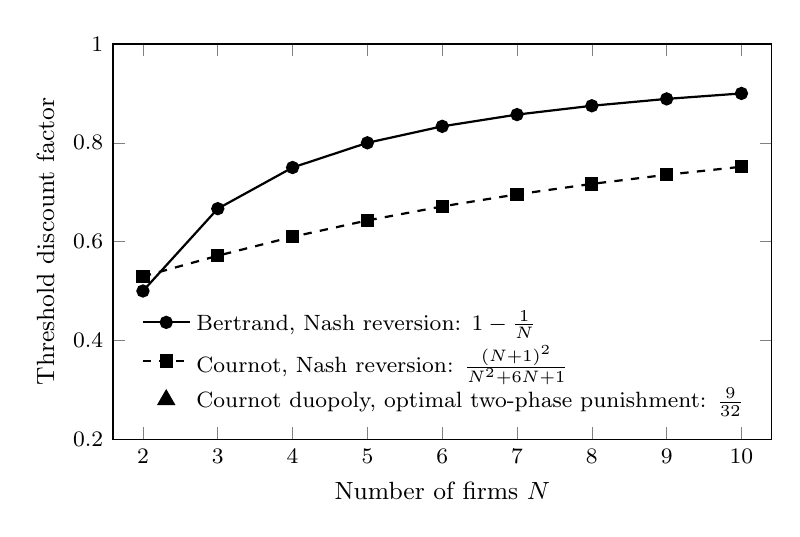
\begin{tikzpicture}
\begin{axis}[
  width=0.82\textwidth, height=6.6cm,
  xmin=1.6, xmax=10.4, ymin=0.2, ymax=1.0,
  xtick={2,3,4,5,6,7,8,9,10},
  xlabel={Number of firms $N$}, ylabel={Threshold discount factor},
  tick label style={font=\footnotesize}, label style={font=\small},
  legend style={at={(0.98,0.04)}, anchor=south east, font=\footnotesize, draw=none, fill=white},
  legend cell align=left]
\addplot[thick, mark=*, samples at={2,3,4,5,6,7,8,9,10}] {1 - 1/x};
\addlegendentry{Bertrand, Nash reversion: $1 - \frac{1}{N}$}
\addplot[thick, dashed, mark=square*, mark options={solid}, samples at={2,3,4,5,6,7,8,9,10}]
  {(x+1)^2/(x^2+6*x+1)};
\addlegendentry{Cournot, Nash reversion: $\frac{(N+1)^2}{N^2+6N+1}$}
\addplot[only marks, mark=triangle*, mark size=3.5pt] coordinates {(2,0.28125)};
\addlegendentry{Cournot duopoly, optimal two-phase punishment: $\frac{9}{32}$}
\end{axis}
\end{tikzpicture}
\caption{Minimum discount factors for collusion at the monopoly outcome. The Bertrand threshold is from
\cref{prop:12-bertrand} and the Cournot threshold, for linear demand, from \cref{prop:12-cournot}. The triangle is the
threshold for the linear Cournot duopoly with the optimal stick-and-carrot punishment of \cref{ex:12-abreu-linear}.}
\label{fig:12-critical-delta}
\end{figure}

Unlike the Bertrand supergame, the Cournot supergame allows partial collusion. When firms are too impatient to
sustain the monopoly output, they can still sustain outputs between the monopoly and Cournot levels.

\begin{proposition}[Partial collusion in linear Cournot]\label{prop:12-partial-cournot}
In the setting of \cref{prop:12-cournot}, let $\delta < \delta^*(N)$ and consider grim trigger with a symmetric
collusive output $q$ between $q^m$ and the Cournot output $q^N$. The profile is an SPE if and only if
$q \ge q(\delta)$, where
\begin{equation}\label{eq:12-partial-q}
q(\delta) = \frac{a - c}{b(N + 1)}\cdot\frac{(N + 1)^2(1 - \delta) + 4\delta}{(N + 1)^2(1 - \delta) + 4N\delta} .
\end{equation}
The output $q(\delta)$ falls continuously from $q^N$ at $\delta = 0$ to $q^m$ at $\delta = \delta^*(N)$. The most
profitable sustainable symmetric output is $q(\delta)$, and the corresponding profit rises continuously from $\pi^N$
to $\pi^c$ as $\delta$ rises from $0$ to $\delta^*(N)$.
\end{proposition}

\begin{proof}
Outputs scale with $\frac{a - c}{b}$ and profits with $k$, while the incentive constraint is homogeneous in profits.
We may therefore set $a - c = 1$ and $b = 1$ and restore the scale at the end. Then
\begin{equation*}
\pi(q) = q(1 - Nq), \qquad \pi^d(q) = \frac{\bigl[1 - (N - 1)q\bigr]^2}{4}, \qquad \pi^N = \frac{1}{(N + 1)^2} ,
\end{equation*}
where $\pi^d(q)$ follows from the best response $\frac{1 - (N - 1)q}{2}$, as in the proof of \cref{prop:12-cournot}.
The incentive constraint is $\pi^d(q) - \pi(q) \le \frac{\delta}{1 - \delta}\bigl[\pi(q) - \pi^N\bigr]$. Its left side
is
\begin{align*}
\pi^d(q) - \pi(q)
&= \frac{1 - 2(N - 1)q + (N - 1)^2q^2 - 4q + 4Nq^2}{4} \\
&= \frac{1 - 2(N + 1)q + (N + 1)^2q^2}{4}
= \frac{\bigl[1 - (N + 1)q\bigr]^2}{4} .
\end{align*}
The profit difference on the right side factors as
\begin{equation*}
\pi(q) - \pi^N = q - Nq^2 - \frac{1}{(N + 1)^2} = N\left(\frac{1}{N + 1} - q\right)\left(q - \frac{1}{N(N + 1)}\right) ,
\end{equation*}
as expanding the product confirms. Now substitute $u = 1 - (N + 1)q$, which runs from $0$ at $q = q^N$ to
$u^m = \frac{N - 1}{2N}$ at $q = q^m = \frac{1}{2N}$. Then $\frac{1}{N + 1} - q = \frac{u}{N + 1}$ and
$q - \frac{1}{N(N + 1)} = \frac{N - 1 - Nu}{N(N + 1)}$, so
\begin{equation*}
\pi(q) - \pi^N = \frac{u\,(N - 1 - Nu)}{(N + 1)^2} .
\end{equation*}
The incentive constraint becomes
\begin{equation*}
\frac{u^2}{4} \le \frac{\delta}{1 - \delta}\cdot\frac{u\,(N - 1 - Nu)}{(N + 1)^2} .
\end{equation*}
At $u = 0$ both sides vanish. For $u > 0$, multiply both sides by $\frac{4(1 - \delta)(N + 1)^2}{u} > 0$:
\begin{align*}
(1 - \delta)(N + 1)^2\,u &\le 4\delta\,(N - 1 - Nu) , \\
u\,\bigl[(1 - \delta)(N + 1)^2 + 4N\delta\bigr] &\le 4\delta(N - 1) , \\
u &\le \bar u(\delta) \equiv \frac{4\delta(N - 1)}{(1 - \delta)(N + 1)^2 + 4N\delta} .
\end{align*}
The constraint is linear in $u$, so the sustainable outputs form the interval $u \in [0, \bar u(\delta)]$, that is,
$q \ge \frac{1 - \bar u(\delta)}{N + 1}$. Since
\begin{equation*}
1 - \bar u(\delta) = \frac{(1 - \delta)(N + 1)^2 + 4N\delta - 4\delta(N - 1)}{(1 - \delta)(N + 1)^2 + 4N\delta}
= \frac{(1 - \delta)(N + 1)^2 + 4\delta}{(1 - \delta)(N + 1)^2 + 4N\delta} ,
\end{equation*}
restoring the scale gives \eqref{eq:12-partial-q}. Writing
$\bar u(\delta) = \frac{4(N - 1)}{(N + 1)^2\frac{1 - \delta}{\delta} + 4N}$ shows that $\bar u$ is continuous and
increasing, with $\bar u(0) = 0$. It reaches $u^m$ where $8N\delta = (1 - \delta)(N + 1)^2 + 4N\delta$, that is, at
$\delta = \frac{(N + 1)^2}{(N + 1)^2 + 4N} = \delta^*(N)$. Finally, $\pi(q)$ decreases in $q$ on $[q^m, q^N]$, so the
most profitable sustainable output is the smallest one, $q(\delta)$.
\end{proof}

A numerical example shows how much collusion impatient firms can sustain. Take $N = 2$ and $\delta = 0.4$, below the
threshold $\frac{9}{17}$, in units with $a - c = 1$ and $b = 1$. Then $\bar u = \frac{1.6}{5.4 + 3.2} = \frac{8}{43}$,
and the most collusive output is $q(0.4) = \frac{1 - \frac{8}{43}}{3} = \frac{35}{129} \approx 0.271$ per firm. This
lies between the monopoly-sharing output 0.25 and the Cournot output 0.333. The margin is
$P - c = 1 - \frac{70}{129} = \frac{59}{129} \approx 0.457$, and each firm earns $\frac{35}{129}\cdot\frac{59}{129}
\approx 0.1241$. Monopoly sharing would give $0.125$ and Cournot $0.1111$, so the firms sustain about 93 percent of
the gain from collusion over Cournot competition. The script \texttt{partial\_cournot.py} confirms these values by
brute force.

\begin{remark}[Repeated play and the conduct parameter]\label{rem:12-conduct}
The menu of conduct in \cref{tab:02-conduct-menu} sets $\theta = 0$ for competition, $\theta = \frac{1}{N}$ for
Cournot and $\theta = 1$ for monopoly. In the linear model the supply relation reads $P - c = \theta\,bQ$. Along the
partial-collusion frontier of \cref{prop:12-partial-cournot}, with $u = \bar u(\delta)$,
\begin{equation*}
\theta(\delta) = \frac{P - c}{bQ} = \frac{1 + N\bar u(\delta)}{N\bigl[1 - \bar u(\delta)\bigr]} ,
\end{equation*}
which rises continuously from $\frac{1}{N}$ at $\delta = 0$ to $1$ at $\delta = \delta^*(N)$. In the example above,
$\theta(0.4) = \frac{59}{70} \approx 0.84$. A conduct parameter estimated from data is thus a summary of the
equilibrium of a dynamic game. If demand or costs change over time, the most collusive equilibrium changes too, and a
constant $\theta$ averages over conduct that varies. This is the critique of \citet{Corts1999} discussed in
\cref{sec:03-corts}. With differentiated products, full collusion is joint profit maximization over all products. It
corresponds to an ownership matrix of ones, $\Omega = \mathbf{1}\mathbf{1}^\top$, in the markup equation
\eqref{eq:04-markup}. The partial internalization weights of \cref{rem:11-mc-theta} are a reduced form for
intermediate conduct.
\end{remark}

\subsection{Optimal punishments}\label{sec:12-optimal-punishment}

Nash reversion is a natural punishment, but in the Cournot game it is far from the harshest credible one. Cournot
profits are positive, while the minmax payoff is zero. \citet{Abreu1986,Abreu1988} showed how to construct the
harshest credible punishments, and that they can be described simply.

\citet{Abreu1988} proves that every SPE outcome path can be supported by a \emph{simple strategy profile}. Such a
profile consists of the desired path and one punishment path for each player. Any unilateral deviation by player
$i$, from any path, starts player $i$'s punishment path from its beginning. Simultaneous deviations by several
players are ignored. The \emph{optimal penal code} uses, for each player, a punishment path that gives that player its
lowest SPE payoff. An outcome path is then an SPE path if and only if no player gains from a one-shot deviation from
it followed by that player's lowest SPE payoff. Harsher credible punishments thus enlarge the set of sustainable
paths, and the worst punishments sustain the most.

For symmetric Cournot supergames, \citet{Abreu1986} shows that, under regularity conditions, the optimal symmetric
punishment has a two-phase \emph{stick-and-carrot} form. In the first phase all firms produce a high output $x$ for one
period, which is the stick. They then return to the most collusive symmetric path, which is the carrot.

\begin{proposition}[Two-phase punishments]\label{prop:12-abreu-two-phase}
Consider $N$ identical Cournot firms, with $\pi(q)$ and $\pi^d(q)$ defined as in \eqref{eq:12-cournot-dev}. Fix a
collusive output $q^c$ and a stick output $x$, and define a profile with two states. In state C every firm produces
$q^c$, and in state P every firm produces $x$. Play starts in state C. After any period in which some firm deviated
from the prescribed output, the next state is P. After any period without a deviation, the next state is C. The
profile is an SPE if and only if
\begin{align}
\pi^d(q^c) - \pi(q^c) &\le \delta\,\bigl[\pi(q^c) - \pi(x)\bigr] , \label{eq:12-carrot}\\
\pi^d(x) - \pi(x) &\le \delta\,\bigl[\pi(q^c) - \pi(x)\bigr] . \label{eq:12-stick}
\end{align}
\end{proposition}

\begin{proof}
We use unnormalized values. The value of state C is $V_C = \frac{\pi(q^c)}{1 - \delta}$, since without deviations the
game stays in C. The value of state P is one period of the stick followed by the carrot, $V_P = \pi(x) + \delta V_C$.
By \cref{prop:12-osdp} we only need to rule out one-shot deviations in each state, and every deviation leads to P.

In state C, the best one-shot deviation earns $\pi^d(q^c)$ and moves the game to P. It is unprofitable if and only if
$\pi^d(q^c) + \delta V_P \le V_C$. Using the expressions for $V_C$ and $V_P$,
\begin{equation*}
V_C - \delta V_P = \frac{\pi(q^c)}{1 - \delta} - \delta\pi(x) - \frac{\delta^2\pi(q^c)}{1 - \delta}
= (1 + \delta)\,\pi(q^c) - \delta\,\pi(x) .
\end{equation*}
The condition $\pi^d(q^c) \le (1 + \delta)\pi(q^c) - \delta\pi(x)$ is \eqref{eq:12-carrot}.

In state P, the best one-shot deviation earns $\pi^d(x)$ and restarts the stick, so the game is again in P. It is
unprofitable if and only if $\pi^d(x) + \delta V_P \le V_P$, that is,
\begin{equation*}
\pi^d(x) \le (1 - \delta)V_P = (1 - \delta)\,\pi(x) + \delta\,\pi(q^c) .
\end{equation*}
Subtracting $\pi(x)$ from both sides gives \eqref{eq:12-stick}.
\end{proof}

The two constraints have clear meanings. The \emph{carrot constraint} \eqref{eq:12-carrot} says that the one-period
gain from cheating on the collusive output must not exceed the loss from spending one period in the stick instead of
the carrot. The \emph{stick constraint} \eqref{eq:12-stick} says that firms must be willing to carry out the
punishment. During the stick each firm would like to cut its output and enjoy the higher price. It refrains because a
deviation would restart the stick and delay the return to collusion. The normalized value of the punishment is
$(1 - \delta)\pi(x) + \delta\pi(q^c)$. The stick can impose a stage profit below the minmax payoff, even a loss. By
\eqref{eq:12-stick}, however, the value of the whole punishment is at least $\pi^d(x)$, which is at least the minmax
payoff.

\begin{example}[Stick and carrot in the linear Cournot duopoly]\label{ex:12-abreu-linear}
Two firms with constant marginal cost $c \ge 0$ face the inverse demand $P(Q) = a - Q$ for every $Q \ge 0$, with
$a > c$. Outputs scale with $a - c$ and profits with $(a - c)^2$, and the thresholds on $\delta$ do not depend on the
scale, so we set $a - c = 1$. The collusive output is $q^c = q^m = \frac{1}{4}$, with
\begin{equation*}
\pi(q^m) = \frac{1}{4}\cdot\frac{1}{2} = \frac{1}{8}, \qquad
\pi^d(q^m) = \left(\frac{1 - \frac{1}{4}}{2}\right)^2 = \frac{9}{64}, \qquad
\pi^d(q^m) - \pi(q^m) = \frac{1}{64} .
\end{equation*}
For a stick output $x \le 1$, the stage profit is $\pi(x) = x(1 - 2x)$ and the best response to $x$ is
$\frac{1 - x}{2}$, so $\pi^d(x) = \frac{(1 - x)^2}{4}$. The gain from deviating during the stick and the loss from the
stick are
\begin{align*}
\pi^d(x) - \pi(x) &= \frac{1 - 2x + x^2 - 4x + 8x^2}{4} = \frac{(3x - 1)^2}{4} , \\
\pi(q^m) - \pi(x) &= \frac{1 - 8x + 16x^2}{8} = \frac{(4x - 1)^2}{8} .
\end{align*}
For $x \ne \frac{1}{4}$, constraints \eqref{eq:12-carrot} and \eqref{eq:12-stick} become $\delta \ge \delta_C(x)$ and
$\delta \ge \delta_S(x)$, with
\begin{equation*}
\delta_C(x) = \frac{\frac{1}{64}}{\frac{(4x - 1)^2}{8}} = \frac{1}{8(4x - 1)^2} , \qquad
\delta_S(x) = \frac{\frac{(3x - 1)^2}{4}}{\frac{(4x - 1)^2}{8}} = \frac{2(3x - 1)^2}{(4x - 1)^2} .
\end{equation*}
For $x < \frac{1}{4}$ the stick raises the price. Then
$\delta_S(x) = 2\left(\frac{1 - 3x}{1 - 4x}\right)^2 \ge 2$, because $1 - 3x \ge 1 - 4x > 0$, so no such stick
works. We therefore take $x > \frac{1}{4}$. A harsher stick lowers $\delta_C$. Beyond the Cournot output $x = \frac{1}{3}$, it raises $\delta_S$, because the
ratio $\frac{3x - 1}{4x - 1}$ has derivative $\frac{1}{(4x - 1)^2} > 0$. On $(\frac{1}{4}, \frac{1}{3}]$ no stick
works, since $\delta_C(x) \ge \delta_C(\frac{1}{3}) = \frac{9}{8} > 1$. For $x \ge 1$ the best response is zero, and
$\delta_S(x) = \frac{2x^2 - x}{2x^2 - x + \frac{1}{8}} \ge \frac{8}{9}$. The lowest discount factor that some stick
can support is therefore attained where the two curves cross on $(\frac{1}{3}, 1)$:
\begin{align*}
\frac{(3x - 1)^2}{4} &= \frac{1}{64} , \\
(3x - 1)^2 &= \frac{1}{16} , \\
48x^2 - 32x + 5 &= 0 .
\end{align*}
The roots are $x = \frac{1}{4}$, which is the collusive output itself, and $x = \frac{5}{12}$. At $x = \frac{5}{12}$,
\begin{equation*}
\pi(x) = \frac{5}{12}\cdot\frac{1}{6} = \frac{5}{72}, \qquad
\pi(q^m) - \pi(x) = \frac{9}{72} - \frac{5}{72} = \frac{1}{18}, \qquad
\underline\delta = \frac{\frac{1}{64}}{\frac{1}{18}} = \frac{18}{64} = \frac{9}{32} .
\end{equation*}
In general units the stick output is $x = \frac{5(a - c)}{12}$ per firm. The stick price is
$\frac{a + 5c}{6}$, still above marginal cost, and each firm earns $\frac{5(a - c)^2}{72}$, below the Cournot profit
$\frac{8(a - c)^2}{72}$. The optimal two-phase punishment sustains monopoly for $\delta \ge \frac{9}{32} \approx
0.281$, against $\frac{9}{17} \approx 0.529$ with Nash reversion. A grid search in \texttt{abreu\_check.py} over
stick outputs confirms the threshold and the stick output for several values of $c$.
\end{example}

\begin{figure}[htbp]
\centering
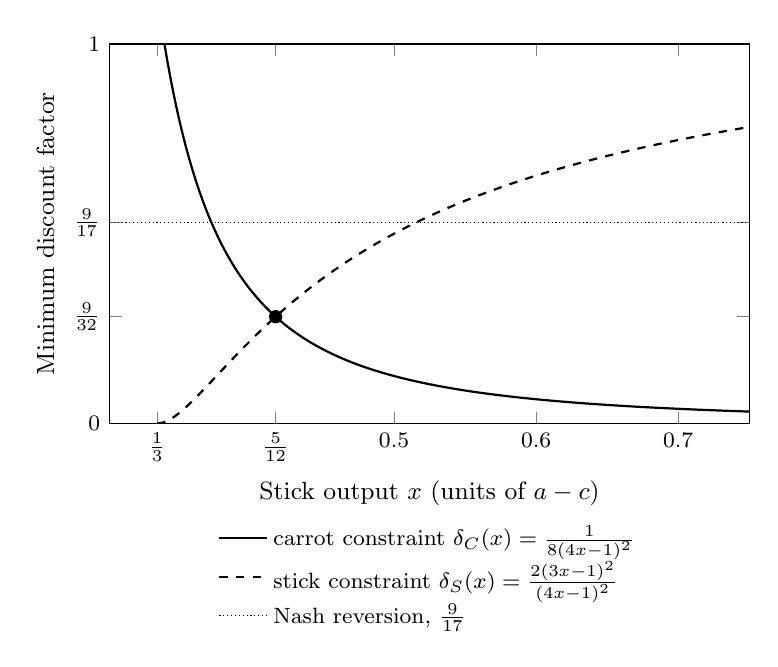
\begin{tikzpicture}
\begin{axis}[
  width=0.8\textwidth, height=6.4cm,
  xmin=0.30, xmax=0.75, ymin=0, ymax=1.0,
  xtick={0.33333,0.41667,0.5,0.6,0.7},
  xticklabels={$\frac{1}{3}$,$\frac{5}{12}$,$0.5$,$0.6$,$0.7$},
  ytick={0,0.28125,0.5294,1},
  yticklabels={$0$,$\frac{9}{32}$,$\frac{9}{17}$,$1$},
  xlabel={Stick output $x$ (units of $a - c$)}, ylabel={Minimum discount factor},
  tick label style={font=\footnotesize}, label style={font=\small},
  legend style={at={(0.5,-0.24)}, anchor=north, font=\footnotesize, draw=none, fill=white},
  legend cell align=left]
\addplot[thick, domain=0.3384:0.75, samples=200] {1/(8*(4*x-1)^2)};
\addlegendentry{carrot constraint $\delta_C(x) = \frac{1}{8(4x - 1)^2}$}
\addplot[thick, dashed, domain=0.33334:0.75, samples=200] {2*(3*x-1)^2/(4*x-1)^2};
\addlegendentry{stick constraint $\delta_S(x) = \frac{2(3x - 1)^2}{(4x - 1)^2}$}
\addplot[densely dotted, domain=0.30:0.75] {9/17};
\addlegendentry{Nash reversion, $\frac{9}{17}$}
\addplot[only marks, mark=*, mark size=2.2pt] coordinates {(0.41667,0.28125)};
\end{axis}
\end{tikzpicture}
\caption{The two constraints of the stick-and-carrot punishment in the linear Cournot duopoly with inverse demand
$a - Q$, from \cref{ex:12-abreu-linear}. A stick output $x$ supports monopoly sharing for every $\delta$ above both
curves. The best stick, $x = \frac{5(a - c)}{12}$, equates the two constraints at $\delta = \frac{9}{32}$.}
\label{fig:12-abreu}
\end{figure}

\Cref{fig:12-abreu} draws the two constraints. A harsher stick makes cheating on the cartel less attractive, but it
also makes the punishment harder to enforce. The best stick balances the two.

\begin{remark}[The price floor and the limit of punishment]\label{rem:12-abreu-floor}
\Cref{ex:12-abreu-linear} treats inverse demand as linear for all outputs, so that very large outputs would drive the
price below zero. The optimal stick keeps the price above marginal cost, but the assumption still matters, because it
determines which sticks are available. Suppose instead that the price cannot fall below zero,
$P(Q) = \max\{a - Q, 0\}$. With $c = 0$, each firm producing at least $a$ drives the price to zero at no cost.
Deviating during such a stick cannot raise the price, so the stick constraint is slack. The carrot constraint
becomes $\frac{1}{64} \le \frac{\delta}{8}$, that is, $\delta \ge \frac{1}{8}$. With $c > 0$, a stick that floods the
market costs $cx$ per period. Our computations with \texttt{abreu\_check.py} show that flooding sticks beat
$\frac{9}{32}$ only when $c < 0.051(a - c)$. Suppose $0 < c \le \frac{a - c}{64}$. A flooding stick in which each
firm produces $\frac{(a - c)^2}{64c}$, earning $-\frac{(a - c)^2}{64}$ per period, then reaches $\delta = \frac{1}{9}$,
provided outputs this large are feasible. At $c = 0$ a stick cannot impose a loss, and the best two-phase code
reaches only $\frac{1}{8}$. No equilibrium can do better than $\frac{1}{9}$. By \cref{lem:12-ir} a deviator's continuation value is at least
the minmax payoff zero, so sustaining monopoly sharing requires $\frac{\pi(q^m)}{1 - \delta} \ge \pi^d(q^m)$, that is,
$\delta \ge 1 - \frac{8}{9} = \frac{1}{9}$. The general lesson is that the harshness of credible punishments depends on
how much damage firms can inflict on one another in a period, and at what cost to themselves.
\end{remark}

In the Bertrand supergame optimal punishments add nothing. Bertrand reversion already holds every firm to its minmax
payoff of zero, which no equilibrium can undercut. Two broader lessons follow from Abreu's analysis. First, the
sustainability of collusion depends on the severity of credible punishments as well as on patience. Second, the most
effective punishment is a short, sharp price war followed by a return to collusion. Wars of this kind reappear in the
models of imperfect monitoring (\cref{sec:12-public}) and in the model of imperfect cartels of \citet{BernheimMadsen2017}
(\cref{sec:13-imperfect}). Stick-and-carrot schemes have one weakness. Once a deviation has occurred, all firms would
gain by skipping the stick and returning to collusion at once. Punishments that are immune to such renegotiation are
milder, which limits how much collusion they can sustain \citep{FarrellMaskin1989}.

\subsection{Asymmetric firms}\label{sec:12-asymmetries}

Symmetric models hide a problem that real cartels face: firms differ, and the collusive agreement must satisfy every
firm's incentive constraint. Consider two Bertrand firms with marginal costs $c_1 < c_2$, and write
$\pi_i(p) = (p - c_i)D(p)$ and $p^m(c_i)$ for firm $i$'s monopoly price. Suppose $c_2 < p^m(c_1)$, so that the cost
advantage is not drastic. The static Bertrand equilibrium then has firm 1 serving the market at a price equal to
$c_2$. Firm 1 earns $\pi_1(c_2) = (c_2 - c_1)D(c_2) > 0$ and firm 2 earns nothing. Let the firms collude on a common
price $p \in (c_2, p^m(c_1)]$ and divide the customers in shares $\alpha_1$ and $\alpha_2 = 1 - \alpha_1$. Undercutting
gives either firm the whole market for one period. With Nash reversion, the normalized incentive constraints are
\begin{equation}\label{eq:12-asym-cost}
\alpha_1\,\pi_1(p) \ge (1 - \delta)\,\pi_1(p) + \delta\,\pi_1(c_2) ,
\qquad
\alpha_2\,\pi_2(p) \ge (1 - \delta)\,\pi_2(p) .
\end{equation}
The efficient firm fears punishment less than its rival, because it keeps a positive profit in the price war. Its
constraint requires $\alpha_1 \ge 1 - \delta + \delta\psi_1$, where $\psi_1 = \frac{\pi_1(c_2)}{\pi_1(p)} \in (0, 1)$,
while firm 2 needs $\alpha_2 \ge 1 - \delta$. Adding the two requirements and using $\alpha_1 + \alpha_2 = 1$ gives
\begin{equation*}
1 \ge 2(1 - \delta) + \delta\psi_1
\quad\Longleftrightarrow\quad
\delta \ge \frac{1}{2 - \psi_1} .
\end{equation*}
The threshold exceeds the symmetric value $\frac{1}{2}$ and rises with the cost gap, which raises $\psi_1$. The cartel
must also give the efficient firm a larger share of the market. In addition, the firms disagree about the price,
since the low-cost firm prefers a lower monopoly price than the high-cost firm.

Without side payments, the firms can still trade price against market share. \citet[section~6.3.2.4,
Exercises~6.1 and~6.5]{Tirole1988} characterizes the efficient trade. Fix a profit target $\bar\pi_2 > 0$ for firm 2.
Both firms charge the price $p$, and firm $i$ produces $s_iD(p)$, with $s_1 + s_2 = 1$. A \emph{constrained-efficient
market-sharing allocation} maximizes firm 1's profit given firm 2's target:
\begin{equation}\label{eq:12-asym-frontier}
\max_{p,\, s_1,\, s_2}\; (p - c_1)\,s_1D(p)
\quad\text{subject to}\quad (p - c_2)\,s_2D(p) \ge \bar\pi_2 , \qquad s_1 + s_2 = 1 .
\end{equation}
Varying $\bar\pi_2$ traces the frontier of profit pairs that the firms can reach without transfers.

\begin{proposition}[Market sharing without side payments]\label{prop:12-asym-sharing}
Let $D$ be positive and decreasing, and let $(p - c)D(p)$ be strictly concave in $p$ for every $c$. Suppose that the
solution of \eqref{eq:12-asym-frontier} has $p > c_2$. Then:
\begin{enumerate}[label=(\roman*)]
\item The price lies between the two monopoly prices, $p^m(c_1) \le p \le p^m(c_2)$.
\item The price solves
\begin{equation}\label{eq:12-asym-foc}
\bigl[(p - c_1)D'(p) + D(p)\bigr] + \frac{(c_2 - c_1)\,\bar\pi_2}{(p - c_2)^2} = 0 .
\end{equation}
\item The price $p$ and firm 2's share $s_2$ both rise with the target $\bar\pi_2$.
\end{enumerate}
\end{proposition}

\begin{proof}
The constraint binds at the optimum, because otherwise moving share to firm 1 raises firm 1's profit. Hence
$s_2 = \frac{\bar\pi_2}{(p - c_2)D(p)}$, and firm 1's profit as a function of $p$ alone is
\begin{equation*}
\Pi_1(p) = (p - c_1)D(p)\,\Bigl[1 - \frac{\bar\pi_2}{(p - c_2)D(p)}\Bigr]
= (p - c_1)D(p) - \frac{(p - c_1)\,\bar\pi_2}{p - c_2} .
\end{equation*}
(i) Strict concavity implies $p^m(c_1) < p^m(c_2)$. For $p < p^m(c_1)$, both $(p - c_1)D(p)$ and $(p - c_2)D(p)$ rise
with $p$. Both factors in the first expression for $\Pi_1$ are then positive and rising, so $\Pi_1$ rises. For
$p > p^m(c_2)$, both factors fall, so $\Pi_1$ falls. The optimum therefore lies in $[p^m(c_1), p^m(c_2)]$.

(ii) The derivative of the last term uses
\begin{equation*}
\frac{\dd}{\dd p}\,\frac{p - c_1}{p - c_2} = \frac{(p - c_2) - (p - c_1)}{(p - c_2)^2} = -\frac{c_2 - c_1}{(p - c_2)^2} .
\end{equation*}
Setting $\Pi_1'(p) = 0$ gives \eqref{eq:12-asym-foc}.

(iii) Let $\Phi(p, \bar\pi_2)$ be the left side of \eqref{eq:12-asym-foc}. The bracket falls with $p$ by strict
concavity, and the second term falls with $p$ for $p > c_2$, so $\frac{\partial\Phi}{\partial p} < 0$. Also
$\frac{\partial\Phi}{\partial\bar\pi_2} = \frac{c_2 - c_1}{(p - c_2)^2} > 0$. By the implicit function theorem,
\begin{equation*}
\frac{\dd p}{\dd\bar\pi_2} = -\frac{\partial\Phi}{\partial\bar\pi_2}\left(\frac{\partial\Phi}{\partial p}\right)^{-1} > 0 .
\end{equation*}
For the share, solve \eqref{eq:12-asym-foc} for $\bar\pi_2$ and substitute it into $s_2$:
\begin{equation*}
s_2 = \frac{-\bigl[(p - c_1)D'(p) + D(p)\bigr]\,(p - c_2)}{(c_2 - c_1)\,D(p)} .
\end{equation*}
On $[p^m(c_1), p^m(c_2)]$ the factor $-[(p - c_1)D'(p) + D(p)]$ is nonnegative and rising, $p - c_2$ is positive and
rising, and $\frac{1}{D(p)}$ is positive and rising. Their product rises with $p$, and hence with $\bar\pi_2$.
\end{proof}

The proposition shows how a cartel without transfers compensates the high-cost firm. To give firm 2 more profit, it
raises the price toward firm 2's preferred level and also gives firm 2 more of the market. Both moves sacrifice
industry profit, because the efficient allocation would let firm 1 serve the market at $p^m(c_1)$. The comparison with
\eqref{eq:12-asym-cost}, where the price was fixed at or below $p^m(c_1)$, shows that efficient sharing uses higher
prices.

Which points of this frontier can grim trigger sustain? Let $\pi_i^*$ be firm $i$'s collusive profit at an
allocation. Firm 1's best deviation charges its own monopoly price $p^m(c_1) \le p$, takes the whole market and earns
$\pi_1(p^m(c_1))$. Bertrand reversion then leaves it $\pi_1(c_2)$ per period. Firm 2's best deviation undercuts $p$
slightly and earns almost $(p - c_2)D(p)$, and reversion leaves it zero. The two constraints are
\begin{equation}\label{eq:12-asym-ic}
\pi_1\bigl(p^m(c_1)\bigr) - \pi_1^* \;\le\; \frac{\delta}{1 - \delta}\bigl[\pi_1^* - \pi_1(c_2)\bigr],
\qquad
(p - c_2)D(p) - \pi_2^* \;\le\; \frac{\delta}{1 - \delta}\,\pi_2^* .
\end{equation}
The first holds only if firm 1's collusive profit is high enough, and the second only if firm 2's is. For a given
$\delta$ only a middle segment of the frontier is sustainable. This is the counterpart, with a variable price, of
\eqref{eq:12-asym-cost}. Tirole adds that the choice among these allocations is itself a coordination problem, which
no symmetry argument can settle when costs differ (section~6.3.2.4).

Capacity asymmetries work through both sides of the constraint. A firm with spare capacity gains much from undercutting
and is hard to punish, because its small rivals cannot flood the market (\cref{ex:12-capacity} and
\citealp{CompteJennyRey2002}). A firm whose incentive constraint is the hardest to satisfy, because of low costs, spare
capacity, or a small share of the collusive profits, constrains what the whole group can sustain. Merger guidelines
call a firm that plays this disruptive role a \emph{maverick} \citep{USDOJFTC2010}. Product differentiation is a
further source of asymmetry, and the next subsection studies its symmetric version.

\subsection{Differentiated products}\label{sec:12-diffprod}

With differentiated products, a firm that undercuts its rivals gains some of their customers but not all, and the
static Nash equilibrium yields positive profits. Both the temptation and the punishment become milder. We work out a
linear duopoly in which the two effects can be compared in closed form.

\begin{proposition}[Collusion with differentiated products]\label{prop:12-diffprod}
Two firms with zero marginal cost face demands $q_i = 1 - p_i + s\,p_j$ for $i \ne j$, with
$0 \le s \le \sqrt 3 - 1 \approx 0.73$. Here $s$ measures substitutability and is not a market share. With grim
trigger and Bertrand-Nash reversion, the joint-profit price is sustainable if and only if
\begin{equation}\label{eq:12-diffprod-delta}
\delta \ge \underline\delta(s) \equiv \frac{(2 - s)^2}{s^2 - 8s + 8} .
\end{equation}
The threshold increases in $s$, from $\frac{1}{2}$ at $s = 0$ to $\frac{3}{5}$ at $s = \sqrt 3 - 1$.
\end{proposition}

\begin{proof}
The model is \cref{ex:04-linear-duopoly} with $a = b = 1$, $d = s$ and $c = 0$. We compute the three profits.

We start with the static Nash equilibrium. Firm $i$ maximizes $p_i(1 - p_i + sp_j)$. The first-order condition
$1 - 2p_i + sp_j = 0$ gives the symmetric equilibrium price $p^N = \frac{1}{2 - s}$. Each firm sells
$1 - (1 - s)p^N = \frac{1}{2 - s}$, so $\pi^N = \frac{1}{(2 - s)^2}$.

Under collusion the firms choose a common price $p$ to maximize $2p\bigl[1 - (1 - s)p\bigr]$. The first-order
condition $1 - 2(1 - s)p = 0$ gives $p^c = \frac{1}{2(1 - s)}$. Each firm sells $\frac{1}{2}$, so
$\pi^c = \frac{1}{4(1 - s)}$.

A firm $i$ that deviates against $p^c$ maximizes $p_i(1 - p_i + sp^c)$, so
\begin{equation*}
p^d = \frac{1 + sp^c}{2} = \frac{1}{2}\left[1 + \frac{s}{2(1 - s)}\right] = \frac{2 - s}{4(1 - s)} .
\end{equation*}
Its sales equal its price, $1 - p^d + sp^c = p^d$, so $\pi^d = (p^d)^2 = \frac{(2 - s)^2}{16(1 - s)^2}$. At this
price the rival sells
\begin{equation*}
1 - p^c + s\,p^d = \frac{4(1 - s) - 2 + s(2 - s)}{4(1 - s)} = \frac{2 - 2s - s^2}{4(1 - s)} ,
\end{equation*}
which is nonnegative if and only if $s \le \sqrt 3 - 1$. For larger $s$ the linear system would assign the rival
negative sales, and the deviation must be computed with the rival's demand truncated at zero.

The threshold \eqref{eq:12-cournot-ic} applies with these profits. The two differences are
\begin{align*}
\pi^d - \pi^c &= \frac{(2 - s)^2 - 4(1 - s)}{16(1 - s)^2} = \frac{s^2}{16(1 - s)^2} , \\
\pi^d - \pi^N &= \frac{(2 - s)^4 - 16(1 - s)^2}{16(1 - s)^2(2 - s)^2}
= \frac{s^2\,(s^2 - 8s + 8)}{16(1 - s)^2(2 - s)^2} ,
\end{align*}
where the second line uses the factorization
\begin{equation*}
(2 - s)^4 - 16(1 - s)^2 = \bigl[(2 - s)^2 - 4(1 - s)\bigr]\bigl[(2 - s)^2 + 4(1 - s)\bigr] = s^2\,(s^2 - 8s + 8) .
\end{equation*}
Their ratio is \eqref{eq:12-diffprod-delta}. The quadratic $s^2 - 8s + 8$ has roots $4 \pm 2\sqrt 2$, both outside $[0, 1]$, so it is
positive on $[0, 1]$. Differentiating,
\begin{equation*}
\frac{d\underline\delta}{ds}
= \frac{-2(2 - s)(s^2 - 8s + 8) - (2 - s)^2(2s - 8)}{(s^2 - 8s + 8)^2}
= \frac{4s(2 - s)}{(s^2 - 8s + 8)^2} > 0
\end{equation*}
for $s \in (0, 1)$. At $s = 0$ the threshold is $\frac{4}{8} = \frac{1}{2}$. At $s = \sqrt 3 - 1$ we have
$(2 - s)^2 = 12 - 6\sqrt 3$ and $s^2 - 8s + 8 = 20 - 10\sqrt 3$, so the threshold is
$\frac{6(2 - \sqrt 3)}{10(2 - \sqrt 3)} = \frac{3}{5}$.
\end{proof}

\begin{figure}[htbp]
\centering
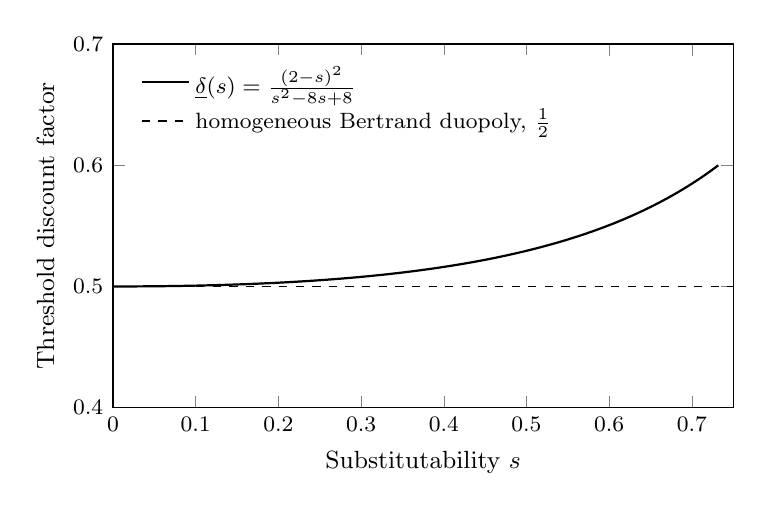
\begin{tikzpicture}
\begin{axis}[
  width=0.78\textwidth, height=6.2cm,
  xmin=0, xmax=0.75, ymin=0.4, ymax=0.7,
  xlabel={Substitutability $s$}, ylabel={Threshold discount factor},
  tick label style={font=\footnotesize}, label style={font=\small},
  legend style={at={(0.03,0.97)}, anchor=north west, font=\footnotesize, draw=none, fill=white},
  legend cell align=left]
\addplot[thick, domain=0:0.732, samples=150] {(2-x)^2/(x^2-8*x+8)};
\addlegendentry{$\underline\delta(s) = \frac{(2 - s)^2}{s^2 - 8s + 8}$}
\addplot[dashed, domain=0:0.75] {0.5};
\addlegendentry{homogeneous Bertrand duopoly, $\frac{1}{2}$}
\end{axis}
\end{tikzpicture}
\caption{Minimum discount factor for collusion at the joint-profit price in the linear differentiated duopoly
$q_i = 1 - p_i + s\,p_j$ with zero cost and Bertrand-Nash reversion (\cref{prop:12-diffprod}).}
\label{fig:12-diffprod-delta}
\end{figure}

\Cref{fig:12-diffprod-delta} plots the threshold. In this specification collusion is easier when products are more
differentiated. Both the gain from deviating and the loss from punishment vanish as $s \to 0$, since
\begin{equation*}
\pi^d - \pi^c = \frac{s^2}{16(1 - s)^2}, \qquad \pi^c - \pi^N = \frac{s^2}{4(1 - s)(2 - s)^2} .
\end{equation*}
The threshold depends on their ratio $R(s) = \frac{(2 - s)^2}{4(1 - s)}$, because
$\underline\delta = \frac{\pi^d - \pi^c}{(\pi^d - \pi^c) + (\pi^c - \pi^N)} = \frac{R}{1 + R}$. The ratio equals one at
$s = 0$ and rises with $s$, so closer substitutes raise the temptation faster than they raise the punishment.
\citet[eq.~(21)]{Deneckere1983} and \citet[eq.~(8)]{Ross1992} derive the same threshold. They state it as the highest
interest rate at which collusion survives, $\frac{1 - \underline\delta}{\underline\delta} = \frac{1}{R(s)} =
\frac{4(1 - s)}{(2 - s)^2}$. Deneckere measures substitutability by the cross-to-own ratio in inverse demand, which
equals $-s$ in our model. Substituting $-s$ for his parameter turns his eq.~(21) into this expression.

Two cautions apply. First, the closed form holds only for $s \le \sqrt 3 - 1$. Beyond that point the deviator's best
price would drive the rival's linear demand below zero. The deviator can take at most the rival's whole market, so
its best deviation then leaves the rival with exactly zero sales. \citet[pp.~40--42]{Deneckere1983} and
\citet[p.~7]{Ross1992} show that with this cap the threshold stops rising. \citet[p.~7]{Ross1992} puts the turning
point near $s = 0.77$. His eq.~(9) gives a highest interest rate of $0.64$ there, so the threshold is
$\frac{1}{1.64} \approx 0.61$. The threshold then falls back toward the homogeneous Bertrand value $\frac{1}{2}$
as $s \to 1$, so the relation is non-monotone over the full range. Second, the answer depends on the model of differentiation. Within the linear
model the threshold depends only on the ratio of the cross-price to the own-price effect, which is $s$ here. The
scale of demand does not matter \citep[p.~7]{Ross1992}. In a spatial model with linear transport costs, where the best
deviation steals only marginal customers, the threshold falls as transport costs rise. A cartel of differentiated
products can then be more stable than one of identical products \citep[pp.~8--11]{Ross1992}.
The general point survives. Differentiation weakens both the temptation to cheat and the punishment, and which effect
dominates depends on the specific model of differentiation \citep[p.~5]{Ross1992}.

\subsection{Coordinated effects of mergers}\label{sec:12-coordinated}

The theory of this section supplies the economics behind the \emph{coordinated effects} of mergers
(\cref{def:11-coordinated}). A merger can make collusion easier through three channels. It removes a firm, which
lowers the threshold. In the Bertrand supergame a merger from $N$ to $N - 1$ firms lowers it from $1 - \frac{1}{N}$
to $1 - \frac{1}{N - 1}$, for example from 0.75 to 0.67 when four firms become three. In the linear Cournot
supergame a merger from three firms to two lowers $\delta^*$ from $\frac{4}{7} \approx 0.571$ to
$\frac{9}{17} \approx 0.529$. In the Bertrand supergame the deviation profit, which is the monopoly profit, and the
punishment profit, which is zero, do not depend on the number of firms. In richer models both fall as firms are
added. A merger then raises both sides of the incentive constraint, and its effect on the threshold is ambiguous in
general \citep[p.~239]{AskerNocke2021}. In the linear Cournot case the net effect lowers the threshold, as the
numbers above show. A merger also changes
asymmetries, and the model of \citet{CompteJennyRey2002} shows how. When the firms other than the largest can serve
the market, the threshold \eqref{eq:12-cjr} is $\frac{\hat K - 1}{\hat K}$, and a merger can only lower it. When
they cannot, the threshold \eqref{eq:12-cjr-large} is $\frac{\hat k_N}{\hat K}$. A merger involving the largest firm
then raises it, while a merger among smaller firms that leaves the largest firm unchanged has no effect. A merger that
creates a large firm with spare capacity, or that gives the merged firm a cost advantage, can thus create a maverick
and make collusion harder. Finally, a merger can eliminate a maverick, which is the case that merger guidelines
emphasize \citep{USDOJFTC2010}. Because the theory has many equilibria, it identifies the conditions under which
coordination is feasible after a merger. It cannot tell us whether coordination will occur. \Cref{sec:11-millercoors}
studies the evidence from the MillerCoors joint venture, where post-merger prices are consistent with coordination
\citep{MillerWeinberg2017}.

Entry interacts with collusion as well. Under perfect collusion with free entry, firms enter until the collusive
profit per firm equals the fixed cost. In the linear Cournot model with a fixed cost $\Phi$ per firm and period,
collusion supports $N^m = \frac{(a - c)^2}{4b\Phi}$ firms, at least as many as Cournot competition with free entry.
Entry then dissipates the whole monopoly rent (\cref{sec:C-cournot}). Consumers gain nothing, because the price stays at the monopoly level. The larger number
of firms also raises the discount factor that collusion requires, since $\delta^*(N^m) > \delta^*(N)$ for any smaller
$N$. Under full collusion the Lerner index is $\frac{a - c}{a + c}$ whatever the number of firms,
so concentration and margins are unrelated under collusion. Cross-industry regressions of margins on concentration
therefore mix industries whose margins respond to concentration (Cournot) with industries whose margins do not
(collusion), as \cref{sec:02-LH,sec:C-cournot} show.

\section{Collusion When Demand Fluctuates}\label{sec:12-demand}

The supergames of \cref{sec:12-perfect} hold demand fixed. Real markets move with the seasons, the business cycle
and shifts in tastes. This section asks how such movements change what a cartel can sustain. The answer rests on
one comparison. In each period a firm weighs the gain from undercutting today against the collusive profit it loses
in the punishment that follows. The gain depends on current demand. The loss depends on expected future demand.
When demand fluctuates, both sides of the incentive constraint move, and they need not move together.

The models of this section differ in how today's demand predicts future demand. If demand shocks are independent
over time and observed by the firms, the future loss is the same in every state, while the gain is largest when
demand is high. Collusion is then hardest in booms, and collusive margins are countercyclical
\citep{RotembergSaloner1986}. If demand follows a predictable cycle, the future loss is small when demand is about
to fall \citep{HaltiwangerHarrington1991}. If booms and recessions are persistent phases of growth, the future loss
is larger in the phase that predicts higher future demand \citep{BagwellStaiger1997}. In all three models firms
observe demand, so the most collusive equilibrium has no price war on its equilibrium path. Price wars on the path
appear when demand is unobserved, the case of \citet{GreenPorter1984} in \cref{sec:12-public}.

Throughout this section $\delta$ is the discount factor. The state of demand in period $t$ is $\omega_t$. The
papers write $\epsilon_t$ for it, a symbol the book reserves for taste shocks. Market demand in state $\omega$ is
$D(p,\omega)$, and industry profit at a common price $p$ is $\pi(p,\omega) = (p-c)D(p,\omega)$. The monopoly price is
$p^m(\omega)$ and monopoly profit is $\pi^m(\omega) = \pi(p^m(\omega),\omega)$. When we quote a paper's equations we
translate them into this notation.

\subsection{A two-state model}\label{sec:12-rs-two-state}

We begin with two demand states. This version shows the logic of \citet{RotembergSaloner1986} in a few lines and
produces four regimes of optimal collusion.

\begin{assumption}[Two independent demand states]\label{asm:12-two-state}
\leavevmode
\begin{enumerate}[label=(\roman*)]
\item $N \ge 2$ firms sell a homogeneous good at constant marginal cost $c$. In each period $t = 0, 1, 2, \dots$ they
set prices simultaneously. The firm with the lowest price serves the market, and firms tied at the lowest price
share it equally.
\item Market demand is $D_H(p)$ in the high state and $D_L(p)$ in the low state. Each state occurs with probability
$\frac{1}{2}$, independently across periods, and $D_H(p) > D_L(p)$ at every price.
\item All firms observe the state before they set prices, and all past prices are observed.
\item Industry profit $\pi_s(p) = (p-c)D_s(p)$ has a unique maximizer $p_s^M$ and is strictly increasing on
$[c, p_s^M]$. We write $\pi_s^M = \pi_s(p_s^M)$ for $s \in \{H, L\}$.
\item Firms maximize expected discounted profit with discount factor $\delta \in (0,1)$.
\end{enumerate}
\end{assumption}

Since $D_H > D_L$, we have $\pi_H(p) > \pi_L(p)$ at every $p > c$. Hence $\pi_H^M \ge \pi_H(p_L^M) > \pi_L^M$. In
this subsection $H$ and $L$ name states. They are not the Herfindahl index or a number of periods.

The firms consider the strategy profile
\begin{equation}\label{eq:12-two-state-strategy}
p_{it}(h^t) =
\begin{cases}
p_H & \text{if no firm has deviated before } t \text{ and the state is } H,\\
p_L & \text{if no firm has deviated before } t \text{ and the state is } L,\\
c & \text{if some firm has deviated before } t,
\end{cases}
\end{equation}
where $h^t$ records past prices and states. The third line is Bertrand reversion. It gives every firm zero profit,
which is the minmax payoff of the stage game (\cref{lem:12-ir}), so no credible punishment is harsher. We
restrict attention to prices $p_s \in [c, p_s^M]$. A price above $p_s^M$ is never useful. A deviator could then
charge $p_s^M$ and earn $\pi_s^M$. Replacing $p_s$ by the price below $p_s^M$ with the same profit leaves the future
unchanged and lowers the deviation payoff.

\casehead{The incentive constraints}
Let
\begin{equation}\label{eq:12-two-state-V}
V \equiv \frac{1}{2}\pi_H(p_H) + \frac{1}{2}\pi_L(p_L)
\end{equation}
be expected industry profit per period on the collusive path. Consider a period in state $s$ with no earlier
deviation. A firm that conforms earns $\frac{1}{N}\pi_s(p_s)$ today. From tomorrow on it earns $\frac{V}{N}$ per period in
expectation. Because states are independent over time, this expectation does not depend on today's state. The
discounted value of the future is
\begin{equation*}
\sum_{\tau = 1}^{\infty} \delta^{\tau}\frac{V}{N} = \frac{\delta}{1-\delta}\,\frac{V}{N}.
\end{equation*}
The best deviation undercuts to $p_s - \varepsilon'$ for a small $\varepsilon' > 0$. (We write $\varepsilon'$ for the price
cut because $\varepsilon$ is an elasticity.) The deviator serves the whole market and earns $\pi_s(p_s - \varepsilon')$,
which tends to $\pi_s(p_s)$ as $\varepsilon' \to 0$. Afterwards every firm prices at $c$, and the deviator earns zero.
Conforming is optimal if
\begin{equation*}
\pi_s(p_s) \le \frac{1}{N}\pi_s(p_s) + \frac{\delta}{1-\delta}\,\frac{V}{N}.
\end{equation*}
Subtracting $\frac{1}{N}\pi_s(p_s)$ from both sides gives
\begin{equation}\label{eq:12-two-state-ic}
\frac{N-1}{N}\,\pi_s(p_s) \le \frac{\delta}{1-\delta}\,\frac{1}{N}\left[\frac{1}{2}\pi_H(p_H) + \frac{1}{2}\pi_L(p_L)\right],
\qquad s \in \{H, L\}.
\end{equation}

\begin{proposition}[Incentive constraints with two demand states]\label{prop:12-rs-two-state-ic}
Under \cref{asm:12-two-state}, with $p_s \in [c, p_s^M]$ for $s = H, L$, the profile \eqref{eq:12-two-state-strategy}
is a subgame perfect equilibrium if and only if \eqref{eq:12-two-state-ic} holds in both states.
\end{proposition}

\begin{proof}
After a deviation the profile prescribes the static Nash equilibrium in every period, whatever happens. This is
subgame perfect by \cref{prop:12-static-repeat}. On the collusive path, the one-shot deviation principle
(\cref{prop:12-osdp}) lets us check single deviations. A price above $p_s$ sells nothing today and leads to zero
profit forever, so it is never better than conforming. A price $p' < p_s$ earns $\pi_s(p') < \pi_s(p_s)$ today, because
$\pi_s$ is strictly increasing on $[c, p_s^M]$, and zero afterwards. If \eqref{eq:12-two-state-ic} holds, every such
deviation pays strictly less than conforming. If \eqref{eq:12-two-state-ic} fails in state $s$, then
$\pi_s(p_s)$ exceeds the conforming payoff. By continuity, $\pi_s(p')$ also exceeds it for $p'$ close enough to
$p_s$, and that deviation is profitable.
\end{proof}

The left side of \eqref{eq:12-two-state-ic} is the current gain from cheating. It is larger in the high state,
because a deviator steals a larger market. The right side is the future loss from the price war. It is the same in
both states, because independent shocks make tomorrow's expected demand the same whatever happens today. The
temptation is therefore strongest in the high state.

\casehead{Optimal collusion}
Define the \emph{slack factor}
\begin{equation}\label{eq:12-kappa}
\kappa \equiv \frac{\delta}{(1-\delta)(N-1)}.
\end{equation}
It rises with $\delta$, falls with $N$, and equals one exactly when $\delta = \frac{N-1}{N}$, the patience threshold of
\cref{prop:12-bertrand}. Multiplying \eqref{eq:12-two-state-ic} by $\frac{N}{N-1}$ gives
\begin{equation}\label{eq:12-two-state-kappa}
\pi_s(p_s) \le \kappa V, \qquad s = H, L.
\end{equation}
\emph{Optimal collusion} selects the most collusive equilibrium in the sense of \cref{sec:12-folk}: the subgame
perfect equilibrium that maximizes the firms' expected profit $V$. It is
convenient to choose profit levels $v_s = \pi_s(p_s) \in [0, \pi_s^M]$ instead of prices. Because $\pi_s$ is strictly
increasing on $[c, p_s^M]$, each $v_s$ determines $p_s$ uniquely. Substituting $V = \frac{1}{2}(v_H + v_L)$ into
\eqref{eq:12-two-state-kappa} and collecting terms gives
\begin{equation*}
\left(1 - \frac{\kappa}{2}\right) v_H \le \frac{\kappa}{2}\, v_L, \qquad \left(1 - \frac{\kappa}{2}\right) v_L \le \frac{\kappa}{2}\, v_H .
\end{equation*}
If $\kappa \ge 2$ both constraints hold for all profit levels. If $\kappa < 2$ they read $v_H \le r v_L$ and
$v_L \le r v_H$ with $r \equiv \frac{\kappa}{2 - \kappa}$. Problems of this form recur in this section, so we solve them once.

\begin{lemma}[Greatest point of a pair of linked constraints]\label{lem:12-two-constraint}
Let $X_1, X_2 > 0$ and $a_1, a_2 \in (0, +\infty]$, where $a_i = +\infty$ means that the corresponding constraint is
absent. Let
\begin{equation*}
S = \left\{ (x_1, x_2) \in [0, X_1] \times [0, X_2] : x_1 \le a_1 x_2,\ x_2 \le a_2 x_1 \right\}.
\end{equation*}
\begin{enumerate}[label=(\roman*)]
\item If $a_1 a_2 < 1$, then $S = \{(0,0)\}$.
\item If $a_1 a_2 \ge 1$, then $x^* = \left(\min\{X_1, a_1 X_2\},\ \min\{X_2, a_2 X_1\}\right)$ belongs to $S$ and
$x^* \ge x$ componentwise for every $x \in S$. At most one coordinate of $x^*$ lies below its cap $X_i$.
\end{enumerate}
\end{lemma}

\begin{proof}
(i) If $a_1 a_2 < 1$, both $a_i$ are finite. For $x \in S$, $x_1 \le a_1 x_2 \le a_1 a_2 x_1$, so
$(1 - a_1a_2)x_1 \le 0$ and $x_1 = 0$. Then $x_2 \le a_2 x_1 = 0$.

(ii) Every $x \in S$ satisfies $x_1 \le \min\{X_1, a_1 x_2\} \le \min\{X_1, a_1 X_2\} = x_1^*$, and likewise
$x_2 \le x_2^*$. It remains to show $x^* \in S$. Suppose first that both coordinates are capped, $x^* = (X_1, X_2)$.
Then $X_1 \le a_1 X_2$ and $X_2 \le a_2 X_1$, so $x^* \in S$. Suppose next that $a_2 X_1 < X_2$, so
$x^* = (\min\{X_1, a_1X_2\}, a_2 X_1)$. Since $a_1 X_2 > a_1 a_2 X_1 \ge X_1$, the first coordinate equals $X_1$. The
constraints read $X_1 \le a_1 a_2 X_1$, which holds, and $a_2 X_1 \le a_2 X_1$. The case $a_1 X_2 < X_1$ is symmetric.
Both coordinates cannot fall below their caps, because $a_1 X_2 < X_1$ and $a_2 X_1 < X_2$ together imply
$a_1 a_2 < 1$.
\end{proof}

The greatest point maximizes every coordinate at once. It therefore maximizes any objective that increases in both
coordinates, such as the cartel's expected profit.

\begin{proposition}[Four regimes of optimal collusion]\label{prop:12-rs-regimes}
Let \cref{asm:12-two-state} hold and define
\begin{equation}\label{eq:12-kappa-bar}
\bar\kappa \equiv \frac{2\pi_H^M}{\pi_H^M + \pi_L^M} \in (1, 2), \qquad
\bar\delta \equiv \frac{\bar\kappa (N-1)}{1 + \bar\kappa(N-1)}.
\end{equation}
The most collusive equilibrium of the form \eqref{eq:12-two-state-strategy} is as follows.
\begin{enumerate}[label=(\roman*)]
\item \emph{Regime 1} ($\kappa \ge \bar\kappa$, equivalently $\delta \ge \bar\delta$). Firms charge the monopoly price
in both states.
\item \emph{Regime 2} ($1 < \kappa < \bar\kappa$). Firms charge $p_L = p_L^M$. The boom price $p_H < p_H^M$ is the
price on the increasing branch of $\pi_H$ that solves
\begin{equation}\label{eq:12-two-state-regime2}
\pi_H(p_H) = \frac{\kappa\,\pi_L^M}{2 - \kappa}.
\end{equation}
\item \emph{Regime 3} ($\kappa = 1$, equivalently $\delta = \frac{N-1}{N}$). Both constraints bind,
$\pi_H(p_H) = \pi_L(p_L) = \pi_L^M$, so $p_L = p_L^M$ and $p_H < p_L$.
\item \emph{Regime 4} ($\kappa < 1$). Only the competitive outcome $p_H = p_L = c$ is sustainable.
\end{enumerate}
\end{proposition}

\begin{proof}
Apply \cref{lem:12-two-constraint} with $x_1 = v_H$, $x_2 = v_L$, $X_1 = \pi_H^M$ and $X_2 = \pi_L^M$. If
$\kappa \ge 2$, set $a_1 = a_2 = +\infty$, and the greatest point is monopoly in both states. Since $\bar\kappa < 2$,
this case belongs to regime 1. If $\kappa < 2$, set $a_1 = a_2 = r = \frac{\kappa}{2-\kappa}$. Then $r < 1$ exactly
when $\kappa < 1$, and part (i) of the lemma gives regime 4. If $1 \le \kappa < 2$, then $r \ge 1$ and part (ii) gives
\begin{equation*}
v_L^* = \min\{\pi_L^M, r\pi_H^M\} = \pi_L^M, \qquad v_H^* = \min\{\pi_H^M, r\pi_L^M\},
\end{equation*}
where the first equality uses $r\pi_H^M \ge \pi_H^M > \pi_L^M$. The boom profit is capped below $\pi_H^M$ exactly
when $r\pi_L^M < \pi_H^M$. Substituting $r$ and rearranging,
\begin{equation*}
\kappa\,\pi_L^M < (2-\kappa)\,\pi_H^M \iff \kappa\left(\pi_H^M + \pi_L^M\right) < 2\pi_H^M \iff \kappa < \bar\kappa .
\end{equation*}
This yields regimes 1 and 2, with $v_H^* = r\pi_L^M$ in regime 2, which is \eqref{eq:12-two-state-regime2}. At
$\kappa = 1$ we have $r = 1$ and $v_H^* = v_L^* = \pi_L^M$. Then $\pi_H(p_H) = \pi_L(p_L^M) < \pi_H(p_L^M)$. If
$p_L^M \le p_H^M$, monotonicity of $\pi_H$ on $[c, p_H^M]$ gives $p_H < p_L^M$. If $p_L^M > p_H^M$, then
$p_H \le p_H^M < p_L^M$. Either way $p_H < p_L$. Finally, $\kappa \ge \bar\kappa$ means
$\frac{\delta}{1-\delta} \ge \bar\kappa(N-1)$, which rearranges to $\delta \ge \bar\delta$. The greatest point maximizes
$V$, so it is the most collusive equilibrium.
\end{proof}

Two checks are useful. Without fluctuations, $\pi_H^M = \pi_L^M$, so $\bar\kappa = 1$ and $\bar\delta = \frac{N-1}{N}$,
the threshold of the constant-demand Bertrand supergame. With fluctuations, $\bar\kappa - 1 =
\frac{\pi_H^M - \pi_L^M}{\pi_H^M + \pi_L^M}$. The range of discount factors with state-dependent pricing widens with the
dispersion of monopoly profits. The next result says when the boom price lies below the recession price.

\begin{corollary}[Countercyclical prices in regime 2]\label{cor:12-rs-countercyclical}
Suppose $p_L^M \le p_H^M$, so the monopoly price is weakly higher in the high state. In regime 2, $p_H < p_L$ if and
only if $\frac{\kappa}{2-\kappa} < \frac{\pi_H(p_L^M)}{\pi_L^M}$. The right side exceeds one, so the boom price is below the
recession price for all $\kappa$ in an interval above one. If instead $p_L^M > p_H^M$, then $p_H < p_L$ throughout
regimes 2 and 3.
\end{corollary}

\begin{proof}
In regime 2, $p_L = p_L^M$, and both $p_H$ and $p_L^M$ lie in $[c, p_H^M]$, where $\pi_H$ is strictly increasing. So
$p_H < p_L^M$ if and only if $\pi_H(p_H) < \pi_H(p_L^M)$. By \eqref{eq:12-two-state-regime2} this is
$\frac{\kappa}{2-\kappa}\pi_L^M < \pi_H(p_L^M)$. If $p_L^M > p_H^M$, then $p_H \le p_H^M < p_L^M = p_L$.
\end{proof}

\begin{example}[Multiplicative demand shocks]\label{ex:12-rs-multiplicative}
Let $D_s(p) = A_s(1-p)$ with $A_H > A_L > 0$ and $c = 0$. Then $\pi_s(p) = A_s p(1-p)$, so $p_H^M = p_L^M = \frac{1}{2}$ and
$\pi_s^M = \frac{A_s}{4}$. The threshold for full monopoly is $\bar\kappa = \frac{2A_H}{A_H + A_L}$. In regime 2,
\eqref{eq:12-two-state-regime2} becomes
\begin{equation*}
A_H\, p_H(1 - p_H) = \frac{\kappa A_L}{4(2-\kappa)} .
\end{equation*}
The lower root of this quadratic is
\begin{equation}\label{eq:12-two-state-example}
p_H = \frac{1}{2}\left[1 - \sqrt{1 - \frac{\kappa A_L}{(2-\kappa)A_H}}\right] < \frac{1}{2} = p_L .
\end{equation}
The recession price is the monopoly price, and the boom price is strictly lower throughout regime 2. Since $c = 0$,
the price is also the margin $p - c$, so margins are countercyclical. With $N = 2$, $A_H = 1.5$ and $A_L = 1$ we get
$\bar\kappa = 1.2$ and $\bar\delta = \frac{6}{11} \approx 0.545$. At $\kappa = 1$ the boom price is
$\frac{1}{2}\left(1 - \sqrt{1 - \frac{A_L}{A_H}}\right) \approx 0.211$. At $\delta = 0.52$, where $\kappa \approx 1.083$, it is
$p_H \approx 0.270$. \Cref{fig:12-rs-two-state} plots both prices against $\delta$.
\end{example}

\begin{figure}[htbp]
\centering
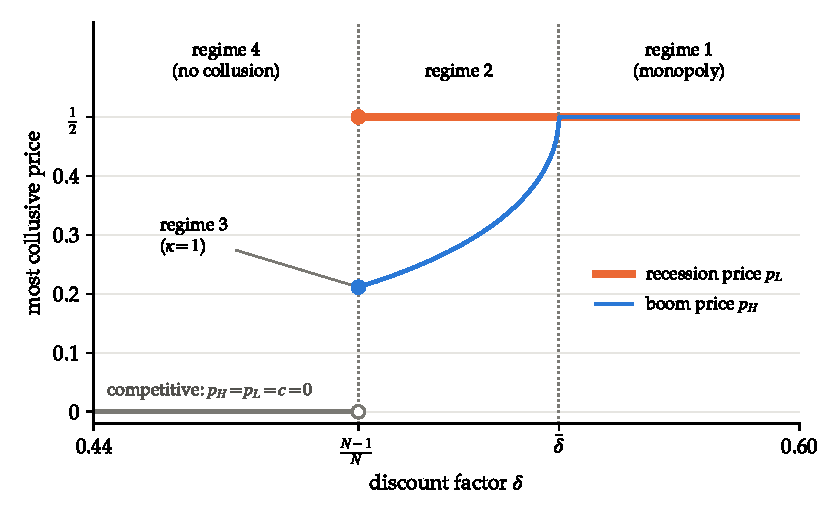
\includegraphics[width=0.78\textwidth]{figures/ch12/rs_two_state.pdf}
\caption{Most collusive prices in the two-state model of \cref{ex:12-rs-multiplicative}: $N = 2$, $c = 0$,
$D_s(p) = A_s(1-p)$ with $A_H = 1.5$ and $A_L = 1$, each state with probability $\frac{1}{2}$. Below
$\delta = \frac{N-1}{N} = \frac{1}{2}$ only competitive pricing is sustainable (regime 4). At $\delta = \frac{1}{2}$ both
constraints bind (regime 3). Between $\frac{1}{2}$ and $\bar\delta = \frac{6}{11}$ the recession price is the monopoly price
$\frac{1}{2}$ and the boom price is lower (regime 2). Above $\bar\delta$ both prices equal $\frac{1}{2}$ (regime 1). Script
\texttt{rs\_two\_state.py}.}
\label{fig:12-rs-two-state}
\end{figure}

\casehead{What the regimes mean}
In regime 2 the cartel concedes in the boom. It lowers the boom price until the gain from undercutting no longer
exceeds the future loss. It keeps the recession price at the monopoly level, because a higher recession profit
raises $V$ and relaxes the boom constraint as well. The result is a pricing pattern that \citet{RotembergSaloner1986}
call a \emph{price war during a boom}: a period of low prices and margins when demand is high. Nobody cheats. The low
boom price is part of the collusive agreement, chosen so that nobody wants to cheat.

Three caveats follow from the proposition. The prediction of countercyclical margins needs optimal collusion. The
competitive outcome is also an equilibrium for every $\delta$, and so is constant pricing at any price that satisfies
both constraints. The prediction also needs intermediate patience. In the example, cyclical pricing occurs only for
$\delta \in [0.5, 0.545)$. Finally, it relies on independent shocks. With persistent demand the future loss depends on
today's state, and the conclusion can reverse, as \cref{sec:12-hh,sec:12-bs} show. Regime 3 is a knife-edge case
with two states. With a continuum of states, profits are capped at a common level in all high states, and this
pattern holds for an interval of discount factors. We turn to that model now.

\subsection{Rotemberg and Saloner (1986): price wars during booms}\label{sec:12-rs}

\subsubsection{The question}

\citet{RotembergSaloner1986} ask how implicitly colluding oligopolists behave when demand fluctuates. Their paper has
two objectives (p.~1). The first is to describe oligopoly pricing over the business cycle. The second is to ask
whether this pricing itself causes business cycles and sticky prices. Their basic point is that collusion is harder
when demand is high. In a boom, ``chiseling away from the collusive level of output becomes more profitable for each
individual firm'' (p.~1), so the oligopoly can sustain only a less collusive outcome. An oligopoly that becomes more
competitive in booms expands output. If its output is an input to other
sectors, their output can rise too. This produces the comovement of outputs that characterizes business cycles.

The question matters for industrial organization because it overturns a piece of folklore. \citet{Scherer1980}
wrote that price cutting ``runs most rampant among oligopolists with high fixed costs'' precisely when business
conditions turn sour (his p.~208, quoted on p.~24). Rotemberg and Saloner concede that one can build models in which recessions
cause price wars. ``Our basis for rejecting this folklore is not theoretical,'' they write. ``Instead our rejection is
based on facts'' (p.~4). We work from the 1984 working paper \citep{RotembergSaloner1984}, which contains the model,
the macroeconomic application and the evidence. Page and table numbers in this subsection refer to it.

\needspace{8\baselineskip}
\subsubsection{The model}

\begin{assumption}[Observable independent demand shocks]\label{asm:12-rs}
\leavevmode
\begin{enumerate}[label=(\roman*)]
\item $N \ge 2$ symmetric firms sell a homogeneous good at constant marginal cost $c$ and set prices simultaneously in
each period. The lowest price serves the market, and ties split it equally.
\item Demand in period $t$ is $D(p, \omega_t)$. The state $\omega_t$ is independent and identically distributed over
time, with CDF $F_\omega$ whose support is $[\underline\omega, \bar\omega]$.
\item All firms learn $\omega_t$ before they set prices, and all past prices are observed.
\item For each $\omega$, $\pi(p,\omega)$ is continuous, strictly increasing in $p$ on $[c, p^m(\omega)]$, and uniquely
maximized at $p^m(\omega)$, with $\pi^m(\omega) > 0$.
\item For each $p > c$, $\pi(p,\omega)$ is strictly increasing in $\omega$. The function $\pi^m$ is continuous and
$\E[\pi^m(\omega)] < \infty$.
\item Firms discount the future with factor $\delta \in (0,1)$.
\end{enumerate}
\end{assumption}

Part (v) says that a higher state shifts demand out. It implies that monopoly profit rises with the state, since for
$\omega' > \omega$ we have $\pi^m(\omega') \ge \pi(p^m(\omega), \omega') > \pi^m(\omega)$. The timing in (iii) is the
model's defining feature. Punishments depend on future states, so their expected size depends on the distribution of
$\omega$. The reward from cheating depends on the current state, which firms see. The authors show that ``for a wide
variety of interesting cases the reward for cheating from the joint profit-maximizing level is monotonically
increasing in $\epsilon_t$'' (pp.~6--7). Here $\epsilon_t$ is the paper's symbol for $\omega_t$.

A \emph{collusive scheme} is a price schedule $p(\cdot)$ that assigns a price to each state. On the collusive path,
every firm charges $p(\omega_t)$. After any deviation, all firms charge $c$ forever. This Nash reversion holds every
firm to its minmax payoff of zero, so it is the harshest credible punishment. Any outcome that some subgame perfect
equilibrium sustains can therefore be sustained with Nash reversion. The authors make the same point about infinite
reversion. ``This length is optimal since it is the biggest credible threat and since, along the equilibrium path,
firms never find themselves punishing each other'' (p.~2). They also note that infinite punishments are less compelling if
industry membership changes, and they use low discount factors in their numerical examples for that reason (p.~8).

As in \cref{sec:12-rs-two-state}, we may restrict attention to $p(\omega) \in [c, p^m(\omega)]$. Write
$v(\omega) = \pi(p(\omega), \omega)$ for industry profit in state $\omega$ on the collusive path, and
$\bar E = \E[v(\omega)]$ for its expectation. The argument that led to \eqref{eq:12-two-state-ic} applies state by
state. A firm that conforms in state $\omega$ earns $\frac{1}{N}v(\omega) + \frac{\delta}{1-\delta}\frac{\bar E}{N}$, and the best
deviation earns $v(\omega)$. The incentive constraint is
\begin{equation*}
\frac{N-1}{N}\, v(\omega) \le \frac{\delta}{1-\delta}\,\frac{\bar E}{N} \qquad \text{for all } \omega.
\end{equation*}
With the slack factor $\kappa$ of \eqref{eq:12-kappa} it reads
\begin{equation}\label{eq:12-rs-ic}
v(\omega) \le \kappa\, \bar E \qquad \text{for all } \omega \in [\underline\omega, \bar\omega].
\end{equation}
The cap $\kappa \bar E$ is the same in every state, because the future does not depend on the present. The cap is
also endogenous. A scheme that earns more on average can afford higher profit in each state.

The paper writes the same condition in terms of the \emph{punishment}
$K = \frac{\delta}{1-\delta}\E[\text{per-firm profit}]$, the expected discounted profit a deviator forfeits (eq.~(1), p.~8).
This $K$ is the paper's symbol and has nothing to do with the capacity of \cref{ex:12-capacity}. A
firm deviates from joint profit maximization in state $\epsilon_t$ if $(N-1)\Pi^m > K$, where $\Pi^m$ is per-firm
monopoly profit (p.~7). The sustainable per-firm profit in high states is $\frac{K}{N-1}$ (eq.~(2), p.~9). In our
notation $K = \frac{\delta \bar E}{(1-\delta)N}$, so the per-firm cap $\frac{K}{N-1}$ equals $\frac{\kappa\bar E}{N}$, which is
\eqref{eq:12-rs-ic} divided by $N$.

\subsubsection{The most collusive scheme as a fixed point}

Every sustainable scheme satisfies $v(\omega) \le \min\{\pi^m(\omega), \kappa\bar E\}$. This suggests the map
\begin{equation}\label{eq:12-rs-h}
h(E) \equiv \E_\omega\left[\min\left\{\pi^m(\omega),\ \kappa E\right\}\right], \qquad E \ge 0,
\end{equation}
which gives the expected profit of the scheme that charges monopoly prices wherever the cap $\kappa E$ allows it.
The map $h$ is continuous and nondecreasing, $h(0) = 0$, and $h(E) \le \E[\pi^m] < \infty$. It is also concave, as
the expectation of a minimum of two functions that are linear in $E$.

\begin{lemma}[Sustainable profit levels]\label{lem:12-rs-fixed}
Under \cref{asm:12-rs}:
\begin{enumerate}[label=(\alph*)]
\item A number $E \ge 0$ is the expected profit of some sustainable scheme if and only if $E \le h(E)$.
\item Let $E^*$ be the largest $E$ with $E \le h(E)$. Then $E^* = h(E^*)$, so $E^*$ is the largest fixed point of $h$.
\item The scheme $v^*(\omega) = \min\{\pi^m(\omega), \kappa E^*\}$ is sustainable. Every sustainable scheme satisfies
$v(\omega) \le v^*(\omega)$ in every state.
\end{enumerate}
\end{lemma}

\begin{proof}
(a) If $v$ is sustainable with mean $E$, then $v(\omega) \le \min\{\pi^m(\omega), \kappa E\}$ for all $\omega$. Taking
expectations, $E \le h(E)$. Conversely, $E = 0$ is the mean of the competitive scheme. If $0 < E \le h(E)$, define
\begin{equation*}
v(\omega) = \frac{E}{h(E)}\min\left\{\pi^m(\omega), \kappa E\right\}.
\end{equation*}
Its mean is $E$. Since $\frac{E}{h(E)} \le 1$, it satisfies $v(\omega) \le \pi^m(\omega)$ and $v(\omega) \le \kappa E$ in every
state. The second inequality is \eqref{eq:12-rs-ic} at mean $E$, so $v$ is sustainable.

(b) The set $\{E \ge 0 : E \le h(E)\}$ is closed, by continuity, and bounded by $\E[\pi^m]$. So it has a largest element
$E^*$. Suppose $E^* < h(E^*)$. Let $E' = h(E^*)$. Since $h$ is nondecreasing, $h(E') \ge h(E^*) = E'$, so $E'$ belongs
to the set and exceeds $E^*$, a contradiction.

(c) Sustainability of $v^*$ follows from (a) and $E^* = h(E^*)$. If $v$ is sustainable with mean $\bar E$, then
$\bar E \le E^*$ by (a) and (b), so $v(\omega) \le \min\{\pi^m(\omega), \kappa\bar E\} \le v^*(\omega)$.
\end{proof}

Part (c) says that the most collusive scheme is the best for the firms in every state at once. There is no tradeoff
between states, so ``most collusive'' is well defined. The paper describes the same construction as a mapping from
punishments to cutoffs and back to punishments, and selects the greatest fixed point (pp.~9--10).

\begin{proposition}[Collusion with observable independent shocks]\label{prop:12-rs-threshold}
Let \cref{asm:12-rs} hold and let $E^*$ be the largest fixed point of $h$.
\begin{enumerate}[label=(\roman*)]
\item If $\kappa < 1$, equivalently $\delta < \frac{N-1}{N}$, then $E^* = 0$. Only competitive pricing is sustainable.
\item If $\kappa = 1$, then $E^* = \pi^m(\underline\omega)$. Industry profit is the same in every state, equal to the
monopoly profit of the lowest state.
\item If $\kappa > 1$, then $E^* > 0$ and $\kappa E^* > \pi^m(\underline\omega)$. Firms charge monopoly prices in every
state if and only if $\kappa\,\E[\pi^m(\omega)] \ge \pi^m(\bar\omega)$. Otherwise there is a cutoff
$\omega^* \in (\underline\omega, \bar\omega)$ with $\pi^m(\omega^*) = \kappa E^*$, and
\begin{equation}\label{eq:12-rs-schedule}
v^*(\omega) =
\begin{cases}
\pi^m(\omega) & \text{if } \omega \le \omega^*,\\
\kappa E^* = \pi^m(\omega^*) & \text{if } \omega > \omega^* .
\end{cases}
\end{equation}
The cutoff solves
\begin{equation}\label{eq:12-rs-cutoff}
\pi^m(\omega^*)\left[1 - \kappa\left(1 - F_\omega(\omega^*)\right)\right] = \kappa \int_{\underline\omega}^{\omega^*} \pi^m(\omega)\, \dd F_\omega(\omega).
\end{equation}
\item The values $E^*$ and $\kappa E^*$ and the cutoff $\omega^*$ are nondecreasing in $\kappa$. They are therefore
nondecreasing in $\delta$ and nonincreasing in $N$.
\end{enumerate}
\end{proposition}

\begin{proof}
(i) If $\kappa < 1$ and $E > 0$, then $h(E) \le \kappa E < E$. So the only fixed point is $E^* = 0$.

(ii) If $\kappa = 1$, then $h(E) = \E[\min\{\pi^m(\omega), E\}] \le E$, with equality if and only if $\pi^m(\omega) \ge E$
with probability one. Because $\underline\omega$ is in the support and $\pi^m$ is continuous and increasing, this
holds if and only if $E \le \pi^m(\underline\omega)$. The fixed points form the interval $[0, \pi^m(\underline\omega)]$,
and the largest is $\pi^m(\underline\omega)$. Then $v^*(\omega) = \min\{\pi^m(\omega), \pi^m(\underline\omega)\} =
\pi^m(\underline\omega)$ in every state.

(iii) Let $\phi(E) = h(E) - E$. For $0 < E \le \frac{\pi^m(\underline\omega)}{\kappa}$, the cap $\kappa E$ lies below
$\pi^m(\omega)$ in every state, so $h(E) = \kappa E$ and $\phi(E) = (\kappa - 1)E > 0$. As $E \to \infty$,
$\phi(E) \le \E[\pi^m] - E \to -\infty$. By continuity $\phi$ has a root above $\frac{\pi^m(\underline\omega)}{\kappa}$,
so $E^* > \frac{\pi^m(\underline\omega)}{\kappa} > 0$.

If $\kappa\E[\pi^m] \ge \pi^m(\bar\omega)$, then $h(\E[\pi^m]) = \E[\pi^m]$, because the cap never binds. No
fixed point exceeds $\E[\pi^m]$, so $E^* = \E[\pi^m]$ and $v^* = \pi^m$. Conversely, if $v^* = \pi^m$ almost surely,
then $E^* = \E[\pi^m]$ and $\pi^m(\omega) \le \kappa\E[\pi^m]$ for almost every $\omega$, hence at $\bar\omega$ by
continuity.

Otherwise $\pi^m(\underline\omega) < \kappa E^* < \pi^m(\bar\omega)$. Since $\pi^m$ is continuous and strictly
increasing, there is a unique $\omega^*$ with $\pi^m(\omega^*) = \kappa E^*$, and $v^*$ takes the form
\eqref{eq:12-rs-schedule}. The fixed-point condition $E^* = h(E^*)$ reads
\begin{equation*}
E^* = \int_{\underline\omega}^{\omega^*} \pi^m(\omega)\, \dd F_\omega(\omega) + \left(1 - F_\omega(\omega^*)\right)\kappa E^* .
\end{equation*}
Substitute $E^* = \frac{\pi^m(\omega^*)}{\kappa}$ and multiply by $\kappa$:
\begin{equation*}
\pi^m(\omega^*) = \kappa\int_{\underline\omega}^{\omega^*} \pi^m(\omega)\, \dd F_\omega(\omega) + \kappa\left(1 - F_\omega(\omega^*)\right)\pi^m(\omega^*).
\end{equation*}
Collecting the terms in $\pi^m(\omega^*)$ gives \eqref{eq:12-rs-cutoff}.

(iv) Write $h_\kappa$ to show the dependence on $\kappa$. For $\kappa' > \kappa$, $h_{\kappa'}(E) \ge h_\kappa(E)$ for all $E$.
So $E^*_\kappa = h_\kappa(E^*_\kappa) \le h_{\kappa'}(E^*_\kappa)$. By \cref{lem:12-rs-fixed}(a) and (b), $E^*_{\kappa'} \ge E^*_\kappa$.
Then $\kappa' E^*_{\kappa'} \ge \kappa E^*_\kappa$, and the cutoff $\omega^* = (\pi^m)^{-1}(\kappa E^*)$ rises weakly. Finally,
$\kappa$ increases in $\delta$ and decreases in $N$.
\end{proof}

Part (i) says that demand fluctuations do not change the patience needed for any collusion at all. Some collusion is
possible exactly when $\delta \ge \frac{N-1}{N}$, as with constant demand. Fluctuations change the form of collusion
above that threshold. Part (iv) restates two claims of the paper (p.~11). The set of states with monopoly pricing
shrinks as $N$ grows, ``as in Stigler's model'' \citep{Stigler1964}. It also shrinks as the future becomes less
important.

\begin{remark}[The existence conditions in the working paper]\label{rem:12-rs-wp}
The working paper states two sufficient conditions for an interior cutoff (pp.~9--10). Its condition (ii) says that
monopoly profit in the highest state exceeds $\kappa$ times its mean, which is the failure of full monopoly in
\cref{prop:12-rs-threshold}(iii). Its condition (i), which should ensure that some collusion is possible, is stated in
a form that appears to come from typographical sign errors in its equations (3) and (5). We have derived the
conditions directly. Collusion is possible if and only if $\kappa \ge 1$, and an interior cutoff exists if and only if
in addition $\kappa\,\E[\pi^m] < \pi^m(\bar\omega)$.
\end{remark}

\subsubsection{The price schedule}

The profit schedule \eqref{eq:12-rs-schedule} translates into prices. Below the cutoff the cartel charges the monopoly
price. Above it, profit must stay at the cap $\kappa E^*$ while demand keeps rising.

\begin{proposition}[Collusive prices fall in booms]\label{prop:12-rs-prices}
Let \cref{asm:12-rs} hold with $\kappa > 1$ and an interior cutoff $\omega^*$. Suppose $\pi$ is continuously
differentiable, $\pi_p > 0$ on $(c, p^m(\omega))$, and $\pi_\omega > 0$ for $p > c$. Let $p^*(\omega)$ be the most
collusive price schedule.
\begin{enumerate}[label=(\roman*)]
\item For $\omega \le \omega^*$, $p^*(\omega) = p^m(\omega)$.
\item For $\omega > \omega^*$, $p^*(\omega)$ is the unique $p \in (c, p^m(\omega))$ with $\pi(p, \omega) = \kappa E^*$, and
\begin{equation}\label{eq:12-rs-dpdw}
\frac{\dd p^*}{\dd \omega} = -\frac{\pi_\omega(p^*, \omega)}{\pi_p(p^*, \omega)} < 0 .
\end{equation}
\item For $\omega > \omega^*$, industry output $D(p^*(\omega), \omega)$ increases in $\omega$.
\item If $p^m$ is nondecreasing, then $p^*$ attains its maximum at $\omega^*$, and the ratio $\frac{p^*(\omega)}{p^m(\omega)}$
decreases strictly on $(\omega^*, \bar\omega]$.
\end{enumerate}
\end{proposition}

\begin{proof}
(i) is \eqref{eq:12-rs-schedule}. For (ii), fix $\omega > \omega^*$. Then $\pi(c, \omega) = 0 < \kappa E^* <
\pi^m(\omega)$. Since $\pi(\cdot, \omega)$ is continuous and strictly increasing on $[c, p^m(\omega)]$, there is exactly
one $p \in (c, p^m(\omega))$ with $\pi(p, \omega) = \kappa E^*$. Differentiate the identity $\pi(p^*(\omega), \omega) =
\kappa E^*$ with respect to $\omega$:
\begin{equation*}
\pi_p(p^*, \omega)\,\frac{\dd p^*}{\dd \omega} + \pi_\omega(p^*, \omega) = 0 .
\end{equation*}
Solving gives \eqref{eq:12-rs-dpdw}. The sign follows from $\pi_\omega > 0$ and $\pi_p > 0$ below the monopoly price. The
implicit function theorem justifies the differentiation because $\pi_p \neq 0$ at $p^*$. For (iii), write
$D(p^*, \omega) = \frac{\kappa E^*}{p^* - c}$. The numerator is constant and the denominator falls. For (iv), $p^*$ rises
weakly up to $\omega^*$ and falls after it. On $(\omega^*, \bar\omega]$ the numerator of $\frac{p^*}{p^m}$ falls while
the denominator does not.
\end{proof}

The intuition is in the paper (pp.~10--11). Above the cutoff, profit is held at the sustainable level. ``If $P$ is
held constant at a level above $c$, the profits from deviating increase. Therefore $P$ must fall. Beyond
$\epsilon_t^*$, prices fall monotonically as $\epsilon_t$ increases.'' Output rises in booms for two reasons:
demand shifts out and the price falls. With multiplicative shocks the monopoly price does not depend on the state, so
the collusive price is constant up to $\omega^*$ and decreasing after it. Prices are then countercyclical over the
whole range of states. With additive shocks the monopoly price rises with demand. The collusive price then rises up
to $\omega^*$ and falls after it.

\casehead{A numerical illustration}
\Cref{fig:12-rs-continuum} computes the most collusive schedule for $N = 2$, $c = 0$ and $\omega \sim U[1,2]$. The script
finds $E^*$ by iterating $E \leftarrow h(E)$ from $E = \E[\pi^m]$. The iterates decrease and converge to the largest
fixed point. In panel (a), demand is $D(p,\omega) = \omega(1-p)$, so $p^m = \frac{1}{2}$ and $\pi^m(\omega) = \frac{\omega}{4}$. Then
$\E[\pi^m] = 0.375$. Full monopoly requires $\kappa \cdot 0.375 \ge \pi^m(2) = \frac{1}{2}$, that is $\kappa \ge \frac{4}{3}$, or
$\delta \ge \frac{4}{7} \approx 0.571$. With the uniform distribution, \eqref{eq:12-rs-cutoff} becomes
\begin{equation*}
\frac{\omega^*}{4}\left[1 - \kappa(2 - \omega^*)\right] = \kappa\int_1^{\omega^*}\frac{\omega}{4}\,\dd\omega = \frac{\kappa\left((\omega^*)^2 - 1\right)}{8}.
\end{equation*}
Multiplying by $\frac{8}{\kappa}$ and collecting terms gives the quadratic
\begin{equation*}
(\omega^*)^2 - \left(4 - \frac{2}{\kappa}\right)\omega^* + 1 = 0,
\end{equation*}
whose larger root is the cutoff. At $\delta = 0.52$, $\kappa \approx 1.083$, $E^* \approx 0.341$, the cap is
$\kappa E^* \approx 0.369$ and $\omega^* \approx 1.477$. The price falls from $\frac{1}{2}$ at the cutoff to about $0.244$
in the highest state. At $\delta = 0.56$ the cutoff moves up to $\omega^* \approx 1.903$, and the price in the highest
state is about $0.390$. In panel (b), demand is $D(p,\omega) = \omega - p$, so $p^m(\omega) = \frac{\omega}{2}$ and
$\pi^m(\omega) = \frac{\omega^2}{4}$. Full monopoly requires $\delta \ge \frac{12}{19} \approx 0.632$. At $\delta = 0.54$ the
cutoff is $\omega^* \approx 1.50$. The price rises to $0.75$ there and then falls to about $0.339$ in the highest state,
where the monopoly price is $1$. At $\delta = 0.60$ the cutoff is $\omega^* \approx 1.855$ and the price peaks at about
$0.927$.

\begin{figure}[htbp]
\centering
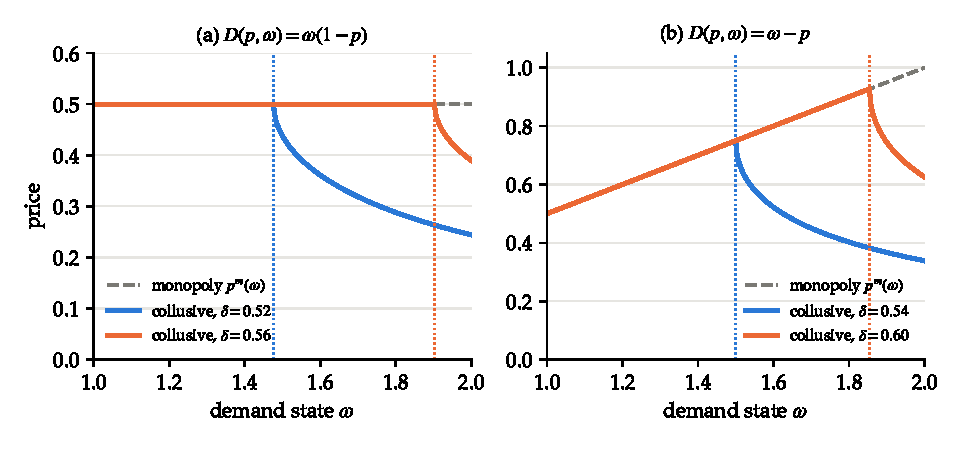
\includegraphics[width=\textwidth]{figures/ch12/rs_continuum.pdf}
\caption{Most collusive price schedules with observable independent demand shocks: $N = 2$, $c = 0$,
$\omega \sim U[1,2]$. Panel (a): multiplicative shocks, $D(p,\omega) = \omega(1-p)$. Panel (b): additive shocks,
$D(p,\omega) = \omega - p$. Dashed: monopoly price $p^m(\omega)$. Solid: collusive price $p^*(\omega)$ for two discount
factors. Dotted vertical lines mark the cutoffs $\omega^*$ of \cref{prop:12-rs-threshold}. Below the cutoff the
collusive price equals the monopoly price. Above it, profit is capped at $\kappa E^*$ and the price falls as demand
rises. Script \texttt{rs\_continuum.py}.}
\label{fig:12-rs-continuum}
\end{figure}

\subsubsection{Collude or compete}

In the optimal scheme no price war is ever observed. The cartel lowers its price smoothly in booms. The paper
also studies a simpler set of strategies in which the cartel can only choose between the monopoly price and the
competitive price (p.~12). Such strategies are ``much simpler and less delicate.'' With this restriction ``the firms
know that when demand is high the monopoly outcome cannot be maintained. They therefore assume that the competitive
outcome will emerge, which is sufficient to fulfill their prophecy.''

Formally, a \emph{collude-or-compete scheme} charges $p^m(\omega)$ in a set $C$ of states and $c$ outside it. In states
outside $C$ all firms charge $c$, a static Nash equilibrium, so nobody wants to deviate there. In a state
$\omega \in C$ the incentive constraint is $\pi^m(\omega) \le \kappa E_R$, where $E_R = \E[\pi^m(\omega)\indic\{\omega \in C\}]$.
Including a low state in $C$ raises $E_R$ without raising the largest profit to be protected. So the best set is an
interval $[\underline\omega, x]$, and the scheme is sustainable if and only if
\begin{equation}\label{eq:12-rs-restricted}
\pi^m(x) \le \kappa\int_{\underline\omega}^{x}\pi^m(\omega)\, \dd F_\omega(\omega).
\end{equation}
A sustainable collude-or-compete scheme is also sustainable in the unrestricted problem. So $E_R \le E^*$, and when
$x$ is interior, $\pi^m(x) \le \kappa E_R \le \kappa E^* = \pi^m(\omega^*)$, so $x \le \omega^*$. The cartel colludes in
fewer states than under the optimal scheme, as the paper states. Above $x$ the price drops from $p^m(x)$ to $c$: an
outright price war, triggered by high demand. This version is the one that connects with empirical studies that
classify periods as collusive or competitive, such as \citet{Bresnahan1987} and \citet{Porter1983}.

\begin{remark}[When do collude-or-compete schemes produce wars?]\label{rem:12-rs-restricted}
Condition \eqref{eq:12-rs-restricted} can fail for every interior $x$ even when the optimal scheme sustains a lot of
collusion. In the two-state model, colluding only in the low state requires $\pi_L^M \le \kappa\cdot\frac{1}{2}\pi_L^M$,
that is $\kappa \ge 2$. But $\bar\kappa < 2$, so for $\kappa \ge 2$ the cartel can already charge monopoly prices in
both states. The restricted scheme is all or nothing. The same happens in both examples of \cref{fig:12-rs-continuum}.
Our computation gives $E_R = 0$ at all four discount factors shown, although the optimal scheme earns between 82 and
almost 100 percent of expected monopoly profit there. The right side of \eqref{eq:12-rs-restricted} is small for $x$ near
$\underline\omega$. A war region at the top therefore requires a distribution in which very high states are rare. Then
the low states accumulate enough profit to protect collusion up to some $x$, and the thin upper tail adds too little
to protect collusion beyond it.
\end{remark}

The shares in the remark are $\frac{0.341}{0.375} \approx 0.91$ and $\frac{0.374}{0.375} \approx 0.997$ in panel (a), and
$\frac{0.479}{0.583} \approx 0.82$ and $\frac{0.573}{0.583} \approx 0.98$ in panel (b).

\subsubsection{Increasing marginal cost}

The model so far assumes constant marginal cost. Increasing marginal cost complicates the model in three ways
(p.~12). First, a price cutter may not want to supply all demand at its price, since it never produces where marginal
cost exceeds price. Second, the profit that the cartel can sustain differs across states, unlike in the constant-cost
case. Third, cheating can take the form of raising price, since rivals that are unwilling to supply all demand at
their price leave some customers for a firm that charges more.

When deviators do not meet all demand, the paper uses the envelope theorem (p.~13). Suppose first that the cartel
charges the monopoly price, which rises with demand. A deviator produces its output $q^d$ where marginal cost equals
the collusive price. By the envelope theorem its profit rises with the state at rate
$q^d\frac{\partial P}{\partial \omega}$, where $P$ is inverse demand. A conforming firm's profit rises at the smaller
rate $q^m\frac{\partial P}{\partial \omega}$, because $q^m < q^d$. Deviation therefore becomes more tempting as demand
rises. Suppose instead that the cartel holds its price fixed as demand rises. The deviation profit then stays fixed.
The conforming profit rises, because the collusive price exceeds marginal cost, and the temptation falls.

When deviators meet all demand, the paper works with the linear example
\begin{equation}\label{eq:12-rs-linear}
P = a + \omega - bQ, \qquad C(q_i) = c\,q_i + \frac{d}{2}q_i^2,
\end{equation}
where $Q$ is industry output and $C$ is each firm's cost (eqs.~(6) and (7)). A cartel that splits output equally
maximizes $(a + \omega - bQ)Q - cQ - \frac{d}{2N}Q^2$. The first-order condition $a + \omega - 2bQ - c - \frac{d}{N}Q = 0$
gives monopoly output and price (eqs.~(8) and (9)):
\begin{equation*}
Q^m = \frac{a + \omega - c}{2b + \frac{d}{N}}, \qquad
P^m = a + \omega - bQ^m = \frac{(a+\omega)(bN + d) + bNc}{2bN + d}.
\end{equation*}
A deviator charging just below $P^m$ would like to produce where $c + dq = P^m$, that is
\begin{equation*}
\bar q = \frac{P^m - c}{d} = \frac{(a + \omega - c)\left(b + \frac{d}{N}\right)}{d\left(2b + \frac{d}{N}\right)}
\end{equation*}
(eq.~(10)). Dividing, $\frac{\bar q}{Q^m} = \frac{b + \frac{d}{N}}{d}$. The deviator meets all demand if and only if
$\bar q \ge Q^m$, that is $b \ge \frac{(N-1)d}{N}$. Marginal cost must not rise too steeply and $N$ must not be too large.
When the deviator meets demand, it sells $Q^m$ at $P^m$ alone, so
\begin{equation*}
\Pi^d = P^mQ^m - cQ^m - \frac{d}{2}(Q^m)^2 .
\end{equation*}
Per-firm collusive profit is $\Pi^m = \frac{1}{N}(P^mQ^m - cQ^m) - \frac{d}{2}\left(\frac{Q^m}{N}\right)^2$. Hence
\begin{equation*}
\Pi^d - N\Pi^m = -\frac{d}{2}(Q^m)^2 + \frac{d}{2N}(Q^m)^2 = \frac{Nd(1-N)}{2}(q^m)^2, \qquad q^m = \frac{Q^m}{N},
\end{equation*}
which is eq.~(11). By the envelope theorem, $\frac{\dd\Pi^m}{\dd\omega} = q^m$. Since $\Pi^d - \Pi^m = (N-1)\Pi^m +
\frac{Nd(1-N)}{2}(q^m)^2$ and $\frac{\dd q^m}{\dd\omega} = \frac{1}{2bN + d}$,
\begin{equation}\label{eq:12-rs-incmc}
\frac{\dd(\Pi^d - \Pi^m)}{\dd\omega} = (N-1)q^m - Nd(N-1)\frac{q^m}{2bN + d} = \frac{(N-1)q^m\left(2bN - d(N-1)\right)}{2bN + d},
\end{equation}
which is eq.~(12). It is positive whenever the deviator meets demand, because then $2bN \ge 2d(N-1) > d(N-1)$. Cheating
becomes more attractive as demand rises.

The paper computes the optimal schedule numerically. For a given punishment, the sustainable price in each state
solves a quadratic equation. The punishment is then updated, starting from a large value and iterating to the first
fixed point (p.~14). Its Figure 1 uses $a = 60$, $b = 1$, $c = 0$, $d = \frac{1}{3}$, $\delta = 0.7$, $N = 5$ and a state
uniform on $\{0, 1, \dots, 80\}$. By eq.~(9) the monopoly price rises linearly from about $30.97$ in state $0$ to about
$72.26$ in state $80$ (our computation). The collusive price equals the monopoly price only in the lowest states. It
then falls, reaches a minimum in the middle of the range of states, and rises slowly at high states. The rise at the
top has a simple cause (p.~15). In high states the collusive price is so low that a deviator would expand only until
price equals its marginal cost. It would no longer serve the whole market. From there, higher demand at a constant
price reduces the temptation, ``thus the oligopoly can afford to increase its prices somewhat.''

\subsubsection{Quantity competition}

With quantities as strategic variables two things change (p.~15). A deviator takes rivals' outputs as given, so its
residual demand is market demand shifted left by their combined output. And the punishment is the Cournot
equilibrium, which yields positive profit. The results are weaker than with prices. Higher demand need not raise the
temptation to cheat. The paper gives a counterexample (p.~16 and its Figure 2). Suppose demand has constant elasticity
and a shock shifts it horizontally. Then the collusive price is the same in both states, and a deviator faces the same
residual demand curve in both, up to a horizontal translation. The extra sales from cheating are the same in both
states, but the revenue lost on the units it would have sold anyway is smaller in the low state. So the incentive to
deviate is strictly larger in the low state. The authors draw a related conclusion: if the cartel keeps its price
constant when demand shifts horizontally, the incentive to cheat falls.

A short calculation makes the counterexample precise. Let marginal cost be a constant $c$, and let $\bar p$ be the
collusive price in both states. In the high state $\omega''$ demand exceeds demand in the low state $\omega'$ by a
constant $k > 0$ at every price. Each firm's collusive output is $q^s(\omega) = \frac{1}{N}D(\bar p,\omega)$, so
$q^s(\omega'') > q^s(\omega')$. Rivals keep producing $(N-1)q^s(\omega)$. A deviator that charges $p < \bar p$
therefore sells $D(p,\omega) - (N-1)q^s(\omega) = q^s(\omega) + y(p)$. The extra sales
$y(p) = D(p,\omega) - D(\bar p,\omega)$ are the same in both states, because the shift $k$ cancels. The deviator's
gain over its conforming profit $\Pi^s(\omega) = (\bar p - c)\,q^s(\omega)$ is
\begin{equation*}
\begin{aligned}
\Pi^d(p,\omega) - \Pi^s(\omega)
&= (p - c)\bigl[q^s(\omega) + y(p)\bigr] - (\bar p - c)\,q^s(\omega) \\
&= (p - c)\,y(p) - (\bar p - p)\,q^s(\omega) .
\end{aligned}
\end{equation*}
The first term is the profit on the extra sales, the equal segments AB and CD of the paper's Figure 2 (p.~16). The
second term is the loss on the units the firm would have sold anyway, and it rises with $q^s(\omega)$. Hence every
deviation price $p < \bar p$ gains strictly more in the low state. If some deviation pays in the high state, the best
deviation pays strictly more in the low state.

With linear demand and cost \eqref{eq:12-rs-linear}, higher demand always raises the temptation. Suppose each firm is
asked to produce $q^s$. A deviator maximizes (eq.~(13))
\begin{equation*}
\Pi^d = q_i\left[a + \omega - c - b\left((N-1)q^s + q_i\right)\right] - \frac{d}{2}q_i^2 ,
\end{equation*}
and the first-order condition gives (eq.~(14))
\begin{equation*}
q^d = \frac{a + \omega - c - b(N-1)q^s}{2b + d} .
\end{equation*}
Let $X = a + \omega - c$ and evaluate at the monopoly output $q^s = q^m = \frac{X}{2bN + d}$. The term in brackets of the
deviator's problem is $A \equiv X - b(N-1)q^m = \frac{X(bN + b + d)}{2bN + d}$, and the deviator earns
$\Pi^d = \frac{A^2}{2(2b + d)}$. A conforming firm earns $\Pi^m = q^m(X - bNq^m) - \frac{d}{2}(q^m)^2 = \frac{X^2}{2(2bN + d)}$.
Subtracting, and using $(bN + b + d)^2 - (2b+d)(2bN + d) = b^2(N-1)^2$,
\begin{equation*}
\Pi^d - \Pi^m = \frac{b^2(N-1)^2 X^2}{2(2b+d)(2bN+d)^2}, \qquad
\frac{\dd(\Pi^d - \Pi^m)}{\dd\omega} = \frac{\left[b(N-1)\right]^2(a + \omega - c)}{(d + 2bN)^2(2b + d)} > 0 .
\end{equation*}
The derivative is the expression on p.~17 of the paper. If the cartel can only collude or compete, high states produce
price wars. If it can choose output freely, it raises output in high states just enough to deter deviation. The
paper's Figure 3 uses $a = 60$, $b = 1$, $c = 0$, $d = \frac{1}{3}$, $\delta = 0.7$ and $N = 5$, the parameters of its
Figure 1. It plots the ratio of the collusive to the monopoly price. The ratio equals one in states up to about 61 and
then falls almost linearly to about $0.92$ in state $80$ (values read from the figure).
The figure's axis is labeled ``Monopoly Price/Oligopoly Price,'' but the text and the plotted values below one
show that it is the oligopoly price relative to the monopoly price. These quantity results hold within Nash-reversion
punishments. In the Cournot supergame harsher credible punishments exist (\cref{sec:12-perfect}), and with them the
cap would be higher.

\subsubsection{From oligopoly pricing to business cycles}

The paper's Section III embeds the oligopoly in a two-sector general equilibrium model (pp.~19--23). Sector 1 is
competitive and sector 2 is the oligopoly. Workers supply any amount of labor at a wage equal to the price of good 1,
and both are normalized to one. Good 1 is produced from labor $L_{1t}$ and an input $Q_{21t}$ of good 2 (p.~19),
\begin{equation}\label{eq:12-rs-ge-prod}
Q_{1t} = A_1Q_{21t} - \frac{B_1}{2}Q_{21t}^2 + G_1L_{1t} - \frac{H_1}{2}L_{1t}^2 .
\end{equation}
Competitive firms equate the price of each input with its marginal revenue product. For good 2 this gives the input
demand
\begin{equation*}
P_{2t} = A_1 - B_1Q_{21t}
\quad\Longleftrightarrow\quad
Q_{21t} = \frac{A_1 - P_{2t}}{B_1} .
\end{equation*}
For labor it gives $G_1 - H_1L_{1t} = 1$, so employment in sector 1 is constant. Consumers' inverse demand for good 2
is $P_{2t} = A_c - B_cQ_{2ct} + e_t$, where $e_t$ is an \iid\ taste shock. Add the two demands,
$Q_{2t} = Q_{21t} + Q_{2ct}$, and solve for $P_{2t}$:
\begin{equation*}
P_{2t} = a + \omega_t - bQ_{2t},
\qquad
a = \frac{A_cB_1 + B_cA_1}{B_c + B_1},
\quad
b = \frac{B_cB_1}{B_c + B_1},
\quad
\omega_t = \frac{B_1}{B_c + B_1}\,e_t .
\end{equation*}
This is the linear demand of \eqref{eq:12-rs-linear}. Producing $Q_{2t}$ requires $cQ_{2t} + \frac{d}{2}Q_{2t}^2$ units of
labor, so marginal cost is $c + dQ_{2t}$ as in the partial-equilibrium model (p.~20).\footnote{Rotemberg and Saloner
write $\alpha$, $\beta$, $\gamma$, $\xi$, $n$, $m$ and $\varepsilon_t$ for our $A_1$, $B_1$, $G_1$, $H_1$, $A_c$, $B_c$ and
$\omega_t$. Their equations (14) and (16) on pp.~19--20 print the labor demand as $\frac{1 + \gamma}{\xi}$ and the
intercept as $\frac{n\beta + m\gamma}{m + \beta}$. The first-order conditions give $\frac{\gamma - 1}{\xi}$ and
$\frac{n\beta + m\alpha}{m + \beta}$. Neither difference affects the argument. The working paper's numbers (13) and
(14) for these equations repeat numbers already used on p.~17, so we cite the section by page.}

The two outputs are linked through the price of good 2. Differentiate \eqref{eq:12-rs-ge-prod} along the input demand:
\begin{equation*}
\frac{\partial Q_{1t}}{\partial P_{2t}}
= \bigl(A_1 - B_1Q_{21t}\bigr)\frac{\partial Q_{21t}}{\partial P_{2t}}
= P_{2t}\cdot\Bigl(-\frac{1}{B_1}\Bigr) < 0 .
\end{equation*}
Output of good 2 is $Q_{2t} = \frac{a + \omega_t - P_{2t}}{b}$, which rises with $\omega_t$ and falls with $P_{2t}$.
Suppose first that sector 2 is competitive, or always acts as a monopolist. Both the competitive and the monopoly
price rise with $\omega_t$, so a taste shift toward good 2 lowers the output of good 1 (p.~20). The two outputs move
in opposite directions, and the economy moves along a production possibility frontier. Suppose instead that the
oligopoly plays the optimal supergame with prices as the strategic variable. A higher $\omega_t$ can then lower
$P_{2t}$ (\cref{sec:12-rs}). Sector 1 buys more of the input and expands, and sector 2 sells more as well. Both
outputs rise together, as all outputs do in a boom (p.~21). Profits can still be procyclical, because revenue minus
total cost can rise with output when there are fixed costs, even as margins fall (p.~22). The authors argue that
this mechanism makes sticky prices and a multiplier natural. They also argue that stabilization
policy could be harmful if booms reflect shifts toward oligopolistic goods. ``If demand for the goods produced by
oligopolies were stable they might collude always, leaving the economy in a permanent recession'' (p.~37).

\subsubsection{The evidence}

Section IV of the paper confronts the folklore with four kinds of evidence (pp.~24--36). None of them is a structural
test. Each asks whether prices or margins in concentrated industries fall when demand is high.

\casehead{The folklore}
\citet{Scherer1980} cites three industries in support of the folklore: rayon, cement and steel. The rayon evidence
shows mainly that the nominal price of rayon fell in the Great Depression, when broad price indices also fell. That
is ``hardly proof of a price war'' (p.~24). For steel, Scherer himself grants that the industry avoided ``widespread
price deterioration, even when operating at less than 65\% capacity between 1958 and 1962'' (p.~24). That leaves
cement.

\casehead{Cement: data and estimating equation}
The data are yearly from 1947 to 1981. The cement price $p^c_t$ is the average price of portland cement from the
Bureau of Mines' \textit{Minerals Yearbook}. It is deflated either by the producer price index $\mathit{PPI}_t$ or by the
price index of construction materials $p^{\mathit{con}}_t$, both from the Bureau of Labor Statistics. The regression
relates the yearly growth rate of the real cement price to the contemporaneous growth rate of GNP. In log-difference
notation,
\begin{equation}\label{eq:12-rs-cement}
\Delta \ln\left(\frac{p^c_t}{P_t}\right) = \beta_0 + \beta_1\, \Delta\ln \mathit{GNP}_t + u_t, \qquad u_t = \phi\, u_{t-1} + e_t,
\qquad P_t \in \left\{\mathit{PPI}_t,\ p^{\mathit{con}}_t\right\}.
\end{equation}
The paper describes the variables as yearly growth rates and does not say whether they are log differences or
percentage changes. Columns (1) and (3) of its Table 1 are ordinary least squares with $\phi = 0$. The Durbin-Watson
statistics of these regressions are low, so columns (2) and (4) re-estimate the equation with first-order
autoregressive errors, ``quasi-differenced'' in the paper's words (p.~25). The paper does not say which feasible
generalized least squares procedure it uses.

The identifying assumption is that GNP growth shifts the demand for cement and is unrelated to the cost and capacity
shocks of the cement industry. The theory predicts $\beta_1 < 0$: when demand grows faster, the collusive price falls
relative to other prices. A competitive industry with rising marginal cost, or a monopoly with procyclical monopoly
prices, would instead show $\beta_1 \ge 0$.

\begin{table}[htbp]
\centering
\caption{The cyclical behavior of real cement prices, yearly data 1947--1981}\label{tab:12-rs-cement}
\small
\begin{tabular}{@{}lcccc@{}}
\toprule
 & (1) & (2) & (3) & (4)\\
Dependent variable: growth of & $\frac{p^c}{\mathit{PPI}}$ & $\frac{p^c}{\mathit{PPI}}$ & $\frac{p^c}{p^{\mathit{con}}}$ & $\frac{p^c}{p^{\mathit{con}}}$\\
\midrule
Constant & 0.025 & 0.025 & 0.038 & 0.037\\
 & (0.010) & (0.012) & (0.007) & (0.008)\\[2pt]
GNP growth, $\beta_1$ & $-0.438$ & $-0.456$ & $-0.875$ & $-0.876$\\
 & (0.236) & (0.197) & (0.161) & (0.149)\\[2pt]
AR(1) coefficient, $\phi$ & & 0.464 & & 0.315\\
 & & (0.173) & & (0.183)\\[2pt]
$R^2$ & 0.10 & 0.15 & 0.48 & 0.52\\
Durbin-Watson & 1.03 & 1.73 & 1.28 & 1.92\\
\bottomrule
\end{tabular}

\smallskip
\begin{minipage}{0.86\textwidth}
\footnotesize
Notes: Estimates of \eqref{eq:12-rs-cement}. $p^c$ is the price of cement, $\mathit{PPI}$ the producer price index and
$p^{\mathit{con}}$ the price index of construction materials. Columns (1) and (3) are ordinary least squares. Columns (2)
and (4) allow first-order autocorrelated errors and are estimated on quasi-differenced data. Standard errors in
parentheses. The paper reports no sample size. Yearly data for 1947--1981 give at most 35 growth rates. Source:
\citet{RotembergSaloner1984}, Table 1.
\end{minipage}
\end{table}

\casehead{Cement: results}
\Cref{tab:12-rs-cement} shows a negative coefficient on GNP growth in all four columns. ``A 1\% increase in the rate of
growth of GNP leads to a 0.5--1.0\% fall in the price of cement'' (p.~25). After the correction for autocorrelation the
coefficients are significant at the 5 percent level. The $t$-ratios are $\frac{-0.456}{0.197} \approx -2.3$ in column (2)
and $\frac{-0.876}{0.149} \approx -5.9$ in column (4). The ordinary least squares standard errors in columns (1) and (3)
are not reliable given the low Durbin-Watson statistics. The anecdotes agree. The real price of cement rose in the
recession years 1954 and 1958 and fell in the boom years 1955 and 1959 (p.~25).

\casehead{Cement: caveats}
The authors raise two objections themselves (pp.~25--26). First, the demand for cement might be only weakly related
to GNP. Cement output growth has a correlation of $0.69$ with GNP growth and $0.77$ with the growth of construction,
which is procyclical. These correlations do not show that cement is more cyclical than the typical sector in GNP.
Without a structural model the question cannot be settled. Second, the regression omits variables a reduced form
should contain, such as the capacity of cement plants. The authors reply that capacity is endogenous and that
adjustment costs make it unresponsive to GNP in the short run. Three further concerns are worth stating. Input costs,
such as energy prices in the 1970s, may move against GNP and enter the cement price directly. If the
construction-materials index in columns (3) and (4) is procyclical, the deflated price is mechanically more
countercyclical, which may explain why those coefficients are larger. And a negative
$\beta_1$ is consistent with any model in which margins fall in booms, including models with capacity constraints or
countercyclical demand elasticities. The regression supports the prediction without isolating the mechanism.

\casehead{Railroads in the 1880s}
\citet{Porter1983} estimated when the railroad cartel on the route from Chicago to New York, the Joint Executive
Committee, was colluding and when it was in a price war. Green and Porter's theory predicts wars after unexpectedly low demand.
Rotemberg and Saloner say that Porter ``finds no support for this theory from the residuals of his estimated
equations'' and argue that his results support their theory instead (p.~26). \Cref{tab:12-rs-railroads} reproduces
their evidence. The first three columns come from Porter's paper. The first is Porter's estimated index of cartel
nonadherence, which parallels closely the contemporary reports in the \textit{Railway Review} and the
\textit{Chicago Tribune}. The second gives rail shipments of wheat from Chicago to New York. The third gives the share
of wheat shipped from Chicago by rail rather than by lake. The last two columns are from the Chicago Board of Trade
annual reports. National grain production adds wheat, corn, rye, oats and barley in tons. The last column counts the
days between April 1 and December 31 on which the Straits of Mackinac were closed to navigation, which prevented
shipment by lake.

\begin{table}[htbp]
\centering
\caption{The railroad cartel, 1880--1886}\label{tab:12-rs-railroads}
\small
\setlength{\tabcolsep}{3pt}
\begin{tabular}{@{}lccccc@{}}
\toprule
 & Estimated & Rail shipments & Fraction shipped & Total grain production & Days lakes closed\\
Year & nonadherence & (million bushels) & by rail (\%) & (billion tons) & (April 1 to Dec.\ 31)\\
\midrule
1880 & 0.00 & 4.73 & 22.1 & 2.70 & 35\\
1881 & 0.44 & 7.68 & 50.0 & 2.05 & 69\\
1882 & 0.21 & 2.39 & 13.8 & 2.69 & 35\\
1883 & 0.00 & 2.59 & 26.8 & 2.62 & 58\\
1884 & 0.40 & 5.90 & 34.0 & 2.98 & 58\\
1885 & 0.67 & 5.12 & 48.5 & 3.00 & 61\\
1886 & 0.06 & 2.21 & 17.4 & 2.83 & 50\\
\bottomrule
\end{tabular}

\smallskip
\begin{minipage}{0.92\textwidth}
\footnotesize
Notes: Columns 1 to 3 are from \citet{Porter1983}, columns 4 and 5 from the Chicago Board of Trade annual reports,
as compiled by Rotemberg and Saloner. Units as printed in the source. The lakes were always closed from January 1 to
March 31. Source: \citet{RotembergSaloner1984}, Table 2.
\end{minipage}
\end{table}

The most severe price wars occurred in 1881, 1884 and 1885. These are the years with the largest rail shipments, in
absolute terms and relative to lake shipments (p.~27). This alone does not show high demand, since shipments may be
high because railroads compete. The authors therefore look at two determinants of demand for rail transport. The
lakes stayed closed longest in 1881 and 1885, the years with the highest nonadherence. In 1883 and 1884 the lakes
were closed only slightly less than in 1885, yet there was a war only in 1884. Grain production explains 1883. It was
the second lowest of the period and 12 percent below 1884 (p.~28). In the authors' words, this ``must have depressed
demand so much that, in spite of the lake closings, total demand for rail transport was low enough to warrant
cooperation.''

The authors anticipate two objections (pp.~28--29). Porter used weekly data, while their table is annual. They reply
that the wars followed a seasonal pattern. The first began around January 1881 and lasted the whole year. The second
began around January 1884 and ended at the end of 1885. Agents could predict the opening of the lakes in midwinter by
studying the thickness of the ice. A railroad that expected a war in the future had two reasons to cut its price at
once. The penalty for deviating was smaller, since the future would be competitive anyway. And shippers who could store
grain would postpone shipments ahead of an expected war, which lowered even the monopoly price. The second objection is
that national grain production is a poor proxy for production in the Chicago region. They reply that national
movements mostly reflect the grain belt, which includes Illinois. The weekly analysis belongs to Porter's own paper and
to \citet{Ellison1994}, who tests Green-Porter against Rotemberg-Saloner with the same data. \Cref{sec:13-jec}
treats both.

\casehead{Automobiles in 1955}
\citet{Bresnahan1987} studies the American automobile industry in the model years 1954 to 1956 (\cref{sec:06-bresnahan}).
Production in 1955 was 44 percent above its 1954 level, and it fell by about 27 percent in 1956
(\cref{tab:06-bres-facts}). The working paper of \citet{RotembergSaloner1984} reports a 45 percent rise and a 44
percent fall (p.~26). The second figure does not match Bresnahan's Table I. Bresnahan finds that a model of
competitive pricing fits the 1955 data, while a collusive model fits 1954 and 1956. Rotemberg and Saloner add that GNP
fell 1 percent in 1954, rose 7 percent in 1955 and rose 2 percent in 1956 (p.~26). In their words, ``Insofar as
cartels can only sustain either competitive or collusive outcomes, this is what our theory predicts'' (p.~26). The
competitive year was the boom year.

\casehead{Price-cost margins}
A direct test would compare prices with marginal costs in booms and recessions. Marginal cost data are scarce, so
industrial organization economists use the \emph{price-cost margin}, sales minus payroll and material costs, divided by
sales. \citet{Scherer1980} summarizes the studies of its cyclical behavior (his p.~357, quoted on p.~29). Concentrated
industries reduce prices, and above all price-cost margins, ``by less in response to a demand slump and increase them
by less in the boom phase.'' The folklore predicts the opposite. Rotemberg and Saloner argue that the fact
favors their theory (p.~30). If part of payroll is a fixed cost, measured margins rise in booms even when price and
marginal cost do not change. Measured margins in concentrated industries rise by less. Either fixed costs matter less
in concentrated industries, which they find unlikely, or concentrated industries cut prices relative to marginal cost
in booms.

\casehead{Product wages and concentration}
The last piece of evidence uses correlations between employment and the \emph{real product wage}. This is the average
hourly wage divided by the industry's value-added deflator. \citet{Burda1984} computed the correlations from detrended
yearly data for 1947--1978. To see why it measures margins, let marginal cost be $mc = \frac{w}{MPL}$, where $w$ is the wage and $MPL$
the marginal product of labor. Then
\begin{equation*}
\frac{w}{p} = MPL \cdot \frac{mc}{p} = MPL\,(1 - L),
\end{equation*}
with $L$ the Lerner index. With constant marginal product, a product wage that rises with employment means a Lerner
index that falls in booms. With diminishing returns, $MPL$ falls in booms, which strengthens the inference (p.~31). The
measure remains valid when part of payroll is fixed. Its weakness is that materials must be proportional to output and
passed through as in a competitive industry (p.~30). The concentration ratio of each two-digit industry is a 1967
sales-weighted average of four-digit four-firm ratios.

\begin{table}[htbp]
\centering
\caption{Concentration and the correlation between real product wages and employment}\label{tab:12-rs-wages}
\small
\setlength{\tabcolsep}{5pt}
\begin{tabular}{@{}llcccc@{}}
\toprule
\multicolumn{6}{@{}l}{\textit{Panel A: two-digit manufacturing industries}}\\
SIC & Industry & Correlation & CR4 & Group & Sign\\
\midrule
\multicolumn{6}{@{}l}{Durables}\\
24 & Lumber and wood products & $-0.33$ & 17.6 & U & $-$\\
25 & Furniture and fixtures & $-0.18$ & 21.6 & U & $-$\\
32 & Stone, clay and glass & 0.39 & 37.4 & C & $+$\\
33 & Primary metals & 0.32 & 42.9 & C & $+$\\
34 & Fabricated metal industries & 0.23 & 29.1 & U & $+$\\
35 & Machinery except electrical & 0.12 & 36.3 & C & $+$\\
36 & Electrical and electronic equipment & 0.34 & 45.0 & C & $+$\\
371 & Motor vehicles and equipment & 0.19 & 80.8 & C & $+$\\
372--9 & Other transportation equipment & 0.02 & 50.1 & C & $+$\\
38 & Instruments and related products & $-0.36$ & 47.8 & C & $-$\\[2pt]
\multicolumn{6}{@{}l}{Nondurables}\\
20 & Food and kindred products & $-0.30$ & 34.5 & U & $-$\\
21 & Tobacco manufactures & $-0.64$ & 73.6 & C & $-$\\
22 & Textile mill products & 0.04 & 34.1 & U & $+$\\
23 & Apparel and related products & $-0.53$ & 19.7 & U & $-$\\
26 & Paper and allied products & $-0.42$ & 31.2 & U & $-$\\
27 & Printing and publishing & 0.40 & 18.9 & U & $+$\\
28 & Chemical and allied products & $-0.03$ & 49.9 & C & $-$\\
29 & Petroleum and coal products & $-0.48$ & 32.9 & U & $-$\\
30 & Rubber & 0.16 & 69.1 & C & $+$\\
31 & Leather and leather products & $-0.44$ & 24.5 & U & $-$\\
\midrule
\multicolumn{6}{@{}l}{\textit{Panel B: contingency table}}\\
 & & Unconcentrated (U) & Concentrated (C) & Total & \\
\midrule
\multicolumn{2}{@{}l}{Negatively correlated} & 7 & 3 & 10 & \\
\multicolumn{2}{@{}l}{Positively correlated} & 3 & 7 & 10 & \\
\multicolumn{2}{@{}l}{Total} & 10 & 10 & 20 & \\
\bottomrule
\end{tabular}

\smallskip
\begin{minipage}{0.9\textwidth}
\footnotesize
Notes: ``Correlation'' is the correlation between the real product wage and employment, detrended yearly data
1947--1978, from \citet{Burda1984}. CR4 is the 1967 four-firm concentration ratio, a sales-weighted average over
four-digit industries (excluding those ending in 99). The groups split the sample at the median concentration of 35.4.
The Group and Sign columns are our classification, and they reproduce Panel B. Source: \citet{RotembergSaloner1984},
Tables 3 and 4.
\end{minipage}
\end{table}

Panel A of \cref{tab:12-rs-wages} shows that concentrated industries such as motor vehicles and electrical equipment
tend to have positive correlations. Unconcentrated ones such as leather, food and wood products tend to have negative
correlations (p.~32). The theory does not say that a slightly more concentrated industry cuts prices more in
booms. A pure monopoly charges the monopoly price, which usually rises with demand. So the authors split the sample at
the median concentration ratio of 35.4, which lies between food and nonelectrical machinery. Panel B gives the
resulting $2 \times 2$ table. Dropping the three industries whose correlations are close to zero (SIC 22, 28 and
372--9) turns the counts 7:3:3:7 into 7:2:2:6. A $\chi^2$ test rejects independence with 92 percent confidence for
Panel B and 97 percent for the reduced table. Fisher's exact test against the alternative that concentrated industries
have more positive correlations rejects with 91 and 96 percent confidence (pp.~33--34). We recomputed these numbers.
The Pearson statistic without continuity correction is $3.20$ ($p = 0.074$) for Panel B and $4.74$ ($p = 0.030$) for the
reduced table. The one-sided Fisher $p$-values are $0.089$ and $0.045$.

\casehead{Alternative explanations}
The authors discuss two (p.~34). Positive correlations could come from monopoly pricing with short-run increasing
returns to labor. They find this unlikely, because firms cut production by closing their least efficient plants
first. Positive correlations could also come from technology shocks that raise labor demand in a sector with upward
sloping labor supply. But the sectors with positive correlations, such as stone, clay and glass, printing and
publishing, and rubber, ``appear to be sectors with fairly stagnant technologies'' (p.~35).

\subsubsection{Critiques and limitations}

The theory and the evidence have limits that later work addressed.
\begin{enumerate}[label=(\arabic*)]
\item \emph{Selection and patience.} Countercyclical pricing describes the most collusive equilibrium for intermediate
discount factors. The competitive equilibrium and many constant-price equilibria exist as well. The theory restricts
what can be sustained, and the prediction rests on the selection.
\item \emph{Independent shocks.} Business cycles are persistent. A boom today predicts high demand tomorrow, which
raises the future loss from a price war exactly when the current gain is large. \Cref{sec:12-hh,sec:12-bs} show
that persistence can reverse the prediction. \citet{Kandori1991} shows that countercyclical pricing survives a family
of correlated shocks when the discount factor is close to a specific value determined by $N$, as summarized by
\citet[p.~2]{BagwellStaiger1995}.
\item \emph{No wars on the path.} With observable demand the optimal scheme lowers prices smoothly. Actual breakdowns
need restricted strategies, and \cref{rem:12-rs-restricted} shows that even then wars at the top require special
distributions. Wars that follow unobserved shocks belong to the theory of \cref{sec:12-public}.
\item \emph{Other forces.} \citet{StaigerWolak1992} add capacity constraints to the model. As Bagwell and Staiger
summarize it, low prices may then be required during downturns, a conclusion analogous to Green and Porter's
\citep[fn.~1]{BagwellStaiger1995}. Storage and intertemporal substitution by buyers, which the authors invoke for the
railroads, also change the incentive constraints.
\item \emph{Reduced-form evidence.} Each piece of evidence shows that margins or prices fall in booms in concentrated
industries. None identifies the mechanism. Capacity, input costs, demand elasticities and fixed costs can produce the
same correlations. The classification by concentration is crude, as the authors note for printing. Its concentration
ratio is low, but its main components, newspapers, books and magazines, are highly concentrated once location and
type are taken into account (p.~32).
\end{enumerate}

\subsubsection{The link to conduct estimation}

Rotemberg-Saloner collusion makes conduct vary with demand. This matters for the conduct-parameter method of
\cref{ch:conduct}. Write the supply relation as
\begin{equation*}
p_t - c_t = \theta_t m_t, \qquad m_t = \frac{Q_t}{\left|\frac{\partial Q_t}{\partial p_t}\right|},
\end{equation*}
where $m_t$ is the markup term. Suppose conduct falls linearly with demand, $\theta_t = \vartheta_0 - \vartheta_1 m_t$
with constants $\vartheta_0$ and $\vartheta_1 > 0$, as in a cartel that concedes in booms. A researcher who estimates
a constant conduct parameter by instrumental variables with a demand shifter recovers a weighted average of the local
slope of the supply relation (\cref{prop:03-corts}). The markup is
$\theta_t m_t = \vartheta_0 m_t - \vartheta_1 m_t^2$, whose slope is $\vartheta_0 - 2\vartheta_1 m_t$. For small
demand movements around $\bar m$ the estimate is close to $\vartheta_0 - 2\vartheta_1\bar m$, while average conduct is
$\vartheta_0 - \vartheta_1\bar m$. The estimate understates market power and can be
negative \citep{Corts1999}. \Cref{sec:03-corts} develops the general result.

\subsubsection{Contribution}

The paper made three lasting contributions. It gave a general logic for collusion under fluctuating demand: compare
the current temptation with the expected future loss, and adjust the collusive price state by state to balance them.
It derived a testable prediction about markups over the cycle, the opposite of the folklore. And it reinterpreted
observed price wars, such as those of 1955 and the 1880s, as consequences of high demand. The papers in the rest of
this section keep the logic and change the demand process.

\subsection{Predictable cycles: Haltiwanger and Harrington (1991)}\label{sec:12-hh}

\citet{HaltiwangerHarrington1991} replace independent shocks with a deterministic demand cycle that firms know in
advance. The original paper is not available to us. We describe its results as \citet[pp.~1--3]{BagwellStaiger1995}
summarize them and develop the logic in our own example. In their framework both the temptation to cheat and the
expected cost of a price war change as the cycle is traversed. They define a boom as a sequence of periods in which
demand rises and a recession as a sequence in which it falls.

\casehead{The incentive constraint}
Let demand in period $t$ be $D_t(p) = A_t d(p)$, where the path $\{A_t\}$ is known to all firms. Let $\pi_t(p) =
(p-c)D_t(p)$ and let $p_t$ be the collusive price at date $t$, with Bertrand reversion forever after a deviation. A
firm that conforms at date $t$ earns $\frac{1}{N}\pi_t(p_t) + \frac{1}{N}\sum_{\tau > t}\delta^{\tau - t}\pi_\tau(p_\tau)$. The best
deviation earns $\pi_t(p_t)$ and then zero. The incentive constraint is
\begin{equation}\label{eq:12-hh-ic}
\frac{N-1}{N}\,\pi_t(p_t) \le \frac{1}{N}\sum_{\tau > t}\delta^{\tau - t}\pi_\tau(p_\tau).
\end{equation}
The right side now depends on the date. Two dates with the same current demand can have very different futures. On
the rising side of the cycle the near future brings higher demand. On the falling side it brings lower demand. The
most collusive path is the greatest solution of $v_t = \min\left\{\pi^m_t, \frac{1}{N-1}\sum_{s \ge 1}\delta^s v_{t+s}\right\}$,
where $v_t = \pi_t(p_t)$ and $\pi^m_t$ is monopoly profit at date $t$. \Cref{lem:13-gas-greatest} in
\cref{ch:collusion-evidence} proves that this greatest solution exists, for punishments of any length.

\begin{example}[A four-period cycle]\label{ex:12-hh-cycle}
Let $D_t(p) = A_t(1-p)$ with $c = 0$, and let $A_t$ cycle through $(4, 8, 12, 8)$. Call the four dates $L$ (low), $M^+$
(middle, rising), $H$ (high) and $M^-$ (middle, falling). Monopoly profits are $\pi^m_t = \frac{A_t}{4}$, so they cycle
through $(\pi_L, \pi_M, \pi_H, \pi_M) = (1, 2, 3, 2)$. Suppose all future dates earn monopoly profits. From $M^+$ the next
four dates bring $(\pi_H, \pi_M, \pi_L, \pi_M)$, and from $M^-$ they bring $(\pi_L, \pi_M, \pi_H, \pi_M)$. The cycle repeats every
four periods, so the future values are
\begin{equation*}
R_{M^+} = \frac{\delta\pi_H + \delta^2\pi_M + \delta^3\pi_L + \delta^4\pi_M}{1 - \delta^4}, \qquad
R_{M^-} = \frac{\delta\pi_L + \delta^2\pi_M + \delta^3\pi_H + \delta^4\pi_M}{1 - \delta^4}.
\end{equation*}
Subtracting,
\begin{equation*}
R_{M^+} - R_{M^-} = \frac{(\delta - \delta^3)(\pi_H - \pi_L)}{1 - \delta^4} = \frac{\delta(\pi_H - \pi_L)}{1 + \delta^2} > 0 .
\end{equation*}
At the same current demand, the future loss from a war is smaller on the falling side. With $N = 2$, monopoly pricing
at each date, holding the others at monopoly, requires $\delta$ of at least $0.313$ at $L$, $0.449$ at $M^+$, $0.621$ at $H$
and $0.548$ at $M^-$ (our computation). At $\delta = 0.58$ only the peak price is cut, to about $0.284$. At $\delta = 0.52$
the most collusive prices at $(L, M^+, H, M^-)$ are about $(0.500, 0.216, 0.124, 0.194)$. At the middle demand level the
price is higher on the rising side, $0.216$, than on the falling side, $0.194$. The script \texttt{hh\_cycle.py} computes
these numbers.
\end{example}

The example shows both forces at work. The peak has the lowest price, which is the Rotemberg-Saloner effect of current
demand. Among dates with equal demand, the price is lower where demand is about to fall, which is the effect that
Haltiwanger and Harrington emphasize. \Cref{sec:13-gas-theory} computes a longer smooth cycle with finite
punishments and reaches the same conclusion.

\casehead{Results}
According to Bagwell and Staiger's summary, Haltiwanger and Harrington show that collusion is most difficult in
recessions, when the cost of a future price war is smallest. They demonstrate that collusive prices are higher in
booms, holding all else equal. The relation between the collusive price and the level of current demand is less clear,
and they cannot give complete analytic results on it. Their simulations show that collusive prices are often
procyclical. As the discount factor drops relative to the number of firms, collusive prices become increasingly
countercyclical, much as Rotemberg and Saloner predicted \citep[p.~2]{BagwellStaiger1995}.

Deterministic cycles suit seasonal demand better than business cycles, whose turning points are hard to predict.
Bagwell and Staiger note this and point to evidence for the Haltiwanger-Harrington model in retail gasoline, where
demand fluctuations are mainly seasonal \citep[fn.~5]{BagwellStaiger1995}. That evidence, \citet{BorensteinShepard1996},
is a deep dive in \cref{sec:13-bs}.

\subsection{Bagwell and Staiger (1997): collusion over the business cycle}\label{sec:12-bs}

\subsubsection{The question}

\citet{BagwellStaiger1997} ask whether collusive prices are procyclical or countercyclical when booms and recessions
are persistent but unpredictable phases. They follow \citet{Hamilton1989} and model the business cycle as a Markov
process that switches between a fast-growth state and a slow-growth state. A \emph{boom} is a period of fast growth in
the level of demand, and a \emph{recession} a period of slow growth. Recessions may, but need not, have negative growth.
Prices are \emph{procyclical} if they are higher in booms and \emph{countercyclical} if they are higher in recessions.
The paper has two main results (WP abstract). Collusive prices may be procyclical (countercyclical) when growth rates
are positively (negatively) correlated over time. And the amplitude of the collusive price cycle is larger when booms
are expected to be shorter and recessions longer. We work from the 1995 working paper
\citep{BagwellStaiger1995} and cite its theorem and equation numbers. We change its notation: $n$ becomes $N$, the
growth rates $b$ and $r$ become $g_b$ and $g_r$, and its value functions $\Omega$, $\omega$, $\tilde\omega_b$, $\tilde\omega_r$
become $\Gamma$, $w$, $W_b$, $W_r$.

\subsubsection{Assumptions and the stationary-growth benchmark}

\begin{assumption}[Bertrand supergame with a growing market]\label{asm:12-bs}
\leavevmode
\begin{enumerate}[label=(\roman*)]
\item $N \ge 2$ firms sell a nondurable homogeneous good in periods $t = 1, 2, \dots$ and set prices
simultaneously. Consumers divide evenly among the lowest-priced firms.
\item The number of consumers in period $t$ is $G_t > 0$, the \emph{level of market demand}. Each consumer has demand
$D(p)$. A lowest-priced firm earns $\pi(p) = (p - c)D(p)$ per consumer it serves. The function $\pi$ has a unique
maximizer $p^m$ and is strictly increasing on $[c, p^m]$. Prices are chosen from $[0, p^m]$.
\item Firms observe all past prices and the current and past levels of demand.
\item Firms use symmetric strategies. The \emph{most collusive prices} are the highest prices supported by a symmetric
subgame perfect equilibrium. Following \citet{Abreu1986}, a deviation is punished by competitive pricing, $p = c$, in
every later period.
\end{enumerate}
\end{assumption}

Here $G_t$ is a level, not a distribution function. The monopoly price is acyclic because it does not depend on the
number of consumers. Any cyclical movement in collusive prices therefore comes from the incentive constraints. Two
per-consumer quantities organize the analysis. A firm that undercuts a common price $p$ captures the whole market, so
its \emph{per-consumer gain from cheating} is
\begin{equation}\label{eq:12-bs-gamma}
\Gamma(p) = \pi(p) - \frac{\pi(p)}{N} = \frac{N-1}{N}\,\pi(p).
\end{equation}
In a war each firm earns $\frac{\pi(c)}{N} = 0$ instead of $\frac{\pi(p)}{N}$. So the \emph{per-consumer, per-period cost of a war} is
\begin{equation}\label{eq:12-bs-w}
w(p) = \frac{\pi(p)}{N} - \frac{\pi(c)}{N} = \frac{\pi(p)}{N}.
\end{equation}

In the \emph{stationary-growth game}, $G_{t+1} = g\,G_t$ with $0 < \delta g < 1$. Demand expands if $g > 1$ and contracts if
$g < 1$. The condition $\delta g < 1$ keeps discounted demand finite. The tradeoff is the same at every date, so a single
most collusive price $p^*$ is charged in every period.

\begin{proposition}[Stationary growth]\label{prop:12-bs-stationary}
In the stationary-growth game, the most collusive price is $p^* = p^m$ if $\delta g \ge \frac{N-1}{N}$ and $p^* = c$
otherwise.
\end{proposition}

\begin{proof}
At date $t$, cheating on a common price $p$ gains $G_t\Gamma(p)$. It costs $G_\tau w(p)$ at every later date $\tau$, and
$G_\tau = g^{\tau - t}G_t$. The incentive constraint is
\begin{equation*}
G_t\,\Gamma(p) \le \sum_{\tau = t+1}^{\infty}\delta^{\tau - t}G_\tau\, w(p) = G_t\sum_{\tau = t+1}^{\infty}(\delta g)^{\tau - t}w(p)
= G_t\,\frac{\delta g}{1 - \delta g}\,w(p).
\end{equation*}
Cancel $G_t$ and substitute \eqref{eq:12-bs-gamma} and \eqref{eq:12-bs-w}:
\begin{equation*}
\frac{N-1}{N}\,\pi(p) \le \frac{\delta g}{1 - \delta g}\,\frac{\pi(p)}{N}.
\end{equation*}
For $p > c$ we may divide by $\frac{\pi(p)}{N} > 0$, which gives $(N-1)(1 - \delta g) \le \delta g$, or $N - 1 \le N\delta g$. This is
$\delta g \ge \frac{N-1}{N}$, and it does not depend on $p$. If it holds, every $p \in (c, p^m]$ is sustainable and the most
collusive price is $p^m$. If it fails, no $p > c$ is sustainable.
\end{proof}

Collusion is easier with more patient firms, fewer firms and faster growth. The ability to collude jumps at
$\delta g = \frac{N-1}{N}$ (WP p.~9). The result matches \cref{prop:12-bertrand-ext}. There demand grows at the net rate
$g$, so the effective discount factor is $\delta(1+g)$. Here $g$ is the gross growth factor, so it is $\delta g$.

\subsubsection{The Markov-growth game}

Demand grows at one of two rates. Period $t$ is a \emph{boom period} if $G_t = g_b G_{t-1}$ and a \emph{recession period}
if $G_t = g_r G_{t-1}$, where $1 > \delta g_b > \delta g_r > 0$. The growth rate $g_t \in \{g_b, g_r\}$ follows a Markov chain with
\begin{equation}\label{eq:12-bs-markov}
\rho \equiv \Pr(g_t = g_r \mid g_{t-1} = g_b), \qquad \lambda \equiv \Pr(g_t = g_b \mid g_{t-1} = g_r).
\end{equation}
So $\rho$ is the probability that a boom turns into a recession and $\lambda$ the probability that a recession turns into a
boom. In this subsection $\rho$ is a transition probability, not pass-through. These parameters fix the expected
durations of the phases. A boom phase that starts in period $t$ lasts exactly $z$ periods with probability
$\rho(1-\rho)^{z-1}$, since it continues $z-1$ times and then ends. Using $\sum_{z \ge 1} z x^{z-1} = \frac{1}{(1-x)^2}$ with
$x = 1 - \rho$, the expected duration is
\begin{equation*}
\sum_{z=1}^{\infty} z\,\rho(1-\rho)^{z-1} = \frac{\rho}{\rho^2} = \frac{1}{\rho}.
\end{equation*}
By the same argument a recession lasts $\frac{1}{\lambda}$ periods on average. The stationary-growth game is the special case
in which booms never end.

\subsubsection{The incentive constraints}

The Markov structure makes the incentives the same in every boom period, whatever the date, and the same in every
recession period. The most collusive prices are therefore a pair, $p_b$ in booms and $p_r$ in recessions. Suppose the
pair $(p_b, p_r)$ is charged forever. Let $W_b$ be a firm's expected discounted profit from period $t+1$ on, per
consumer of period $t+1$, when period $t+1$ is a boom. Define $W_r$ in the same way for a recession. Since
profits fall to zero in a war, $W_b$ and $W_r$ also measure the cost of a war.

Suppose period $t$ is a boom. Next period demand is $g_r G_t$ with probability $\rho$ and $g_b G_t$ with probability $1-\rho$.
The boom incentive constraint is
\begin{equation*}
G_t\,\Gamma(p_b) \le \delta\left[\rho\,(g_r G_t)\,W_r + (1-\rho)\,(g_b G_t)\,W_b\right].
\end{equation*}
The level $G_t$ cancels. Future demand is always proportional to current demand, so the current level is a scaling
factor that does not affect the incentive to collude. The full system is (WP (1)--(4))
\begin{align}
\Gamma(p_b) &\le \delta\left[\rho\, g_r W_r + (1-\rho)\, g_b W_b\right], \label{eq:12-bs-ic-b}\\
\Gamma(p_r) &\le \delta\left[\lambda\, g_b W_b + (1-\lambda)\, g_r W_r\right], \label{eq:12-bs-ic-r}\\
W_b &= w(p_b) + \delta\left[\rho\, g_r W_r + (1-\rho)\, g_b W_b\right], \label{eq:12-bs-W-b}\\
W_r &= w(p_r) + \delta\left[\lambda\, g_b W_b + (1-\lambda)\, g_r W_r\right]. \label{eq:12-bs-W-r}
\end{align}
The first two lines compare today's temptation with the discounted future profit that cheating destroys. The last two
are recursions for that future profit. Write them as a linear system:
\begin{equation*}
\left[1 - (1-\rho)\delta g_b\right] W_b - \rho\,\delta g_r W_r = w(p_b), \qquad
-\lambda\,\delta g_b W_b + \left[1 - (1-\lambda)\delta g_r\right] W_r = w(p_r).
\end{equation*}
Its determinant is $\left[1 - (1-\lambda)\delta g_r\right]\left[1 - (1-\rho)\delta g_b\right] - \delta^2\lambda g_b\rho g_r$. Define
\begin{equation}\label{eq:12-bs-Delta}
\Delta \equiv \frac{\delta}{\left[1 - (1-\lambda)\delta g_r\right]\left[1 - (1-\rho)\delta g_b\right] - \delta^2\lambda g_b \rho g_r}.
\end{equation}
In this subsection $\Delta$ is a scalar, unrelated to the matrix of share derivatives or to the difference operator
of \eqref{eq:12-rs-cement}. The paper shows that $\Delta > 0$ and that $\Delta$ increases in $\delta$ on $(0, \frac{1}{g_b})$ (WP
fn.~7). Cramer's rule gives (WP (5) and (6))
\begin{equation}\label{eq:12-bs-W-solved}
\begin{aligned}
W_b &= \left\{\frac{w(p_b)\left[1 - (1-\lambda)\delta g_r\right]}{\delta} + w(p_r)\rho g_r\right\}\Delta, \\
W_r &= \left\{\frac{w(p_r)\left[1 - (1-\rho)\delta g_b\right]}{\delta} + w(p_b)\lambda g_b\right\}\Delta .
\end{aligned}
\end{equation}

Substitute into the right side of \eqref{eq:12-bs-ic-b}, which is $\delta\rho g_r W_r + \delta(1-\rho)g_b W_b$. The coefficient on
$w(p_r)$ is
\begin{equation*}
\rho g_r\Delta\left[1 - (1-\rho)\delta g_b\right] + (1-\rho)g_b\Delta\,\delta\rho g_r = \rho g_r \Delta .
\end{equation*}
The coefficient on $w(p_b)$ is
\begin{equation*}
g_b\Delta\left[\delta\rho g_r\lambda + (1-\rho)\left(1 - (1-\lambda)\delta g_r\right)\right]
= g_b\Delta\left[1 - \rho - \delta g_r(1 - \lambda - \rho)\right],
\end{equation*}
where the equality uses $(1-\rho)(1-\lambda) - \rho\lambda = 1 - \lambda - \rho$. The recession constraint works the same way. The
two constraints become (WP (8) and (9))
\begin{align}
\Gamma(p_b) &\le \left\{w(p_r)\rho g_r + w(p_b)g_b\left[1 - \rho - \delta g_r(1 - \lambda - \rho)\right]\right\}\Delta, \label{eq:12-bs-8}\\
\Gamma(p_r) &\le \left\{w(p_b)\lambda g_b + w(p_r)g_r\left[1 - \lambda - \delta g_b(1 - \lambda - \rho)\right]\right\}\Delta. \label{eq:12-bs-9}
\end{align}
The future loss is a weighted average of the profit lost in future booms and recessions, with weights that reflect
the expected time spent in each. Substitute $\Gamma = \frac{N-1}{N}\pi$ and $w = \frac{\pi}{N}$, multiply by $N$, and move the own-state
term to the left. The constraints take the form (WP (10)--(13))
\begin{equation}\label{eq:12-bs-10-11}
\pi(p_b)\,\mathcal{B} \le \pi(p_r)\,\rho g_r\Delta, \qquad \pi(p_r)\,\mathcal{R} \le \pi(p_b)\,\lambda g_b\Delta,
\end{equation}
with
\begin{equation}\label{eq:12-bs-B-R}
\mathcal{B} = N - 1 - g_b\Delta\left[1 - \rho - \delta g_r(1 - \lambda - \rho)\right], \qquad
\mathcal{R} = N - 1 - g_r\Delta\left[1 - \lambda - \delta g_b(1 - \lambda - \rho)\right].
\end{equation}
The coefficient $\mathcal B$ is the net temptation in a boom: the gain from cheating minus the part of the future loss
that comes from future boom profits.

\subsubsection{Correlation of growth rates}

In the stationary game the growth rate decides everything. In the Markov game the relevant object is expected future
growth, which may depend on the current phase. One period ahead,
\begin{align*}
\E[G_{t+1} \mid g_t = g_b] - \E[G_{t+1} \mid g_t = g_r]
&= \left[(1-\rho)g_b + \rho g_r - \lambda g_b - (1-\lambda)g_r\right]G_t \\
&= (1 - \lambda - \rho)(g_b - g_r)\,G_t .
\end{align*}
Expected demand next period is higher after a boom if and only if $1 - \lambda - \rho > 0$. What matters for collusion is
discounted demand over the whole future. Normalize $G_t = 1$ and let $\tilde G_b$ be expected discounted demand from period
$t$ on when $t$ is a boom, and $\tilde G_r$ the same for a recession. They satisfy
$\tilde G_b = 1 + \delta\left[\rho g_r\tilde G_r + (1-\rho)g_b\tilde G_b\right]$ and
$\tilde G_r = 1 + \delta\left[\lambda g_b\tilde G_b + (1-\lambda)g_r\tilde G_r\right]$. Solving (WP (14)),
\begin{equation}\label{eq:12-bs-14}
\tilde G_b - \tilde G_r = \Delta\,(g_b - g_r)(1 - \lambda - \rho).
\end{equation}
Growth rates are \emph{positively correlated} if $1 - \lambda - \rho > 0$, \emph{negatively correlated} if $1 - \lambda - \rho < 0$,
and \emph{uncorrelated} if $1 - \lambda - \rho = 0$. Under positive correlation a boom predicts more future demand, so a war
started in a boom costs more. Collusion should then be easier in booms. Under negative correlation the reverse holds.

\subsubsection{The most collusive prices}

The analysis has four parameters besides $(\rho, \lambda)$: $N$, $\delta$, $g_b$ and $g_r$. The first result disposes of the
extreme cases.

\begin{proposition}[Extreme cases]\label{prop:12-bs-extreme}
In the Markov-growth game:
\begin{enumerate}[label=(\roman*)]
\item If $\delta g_r \ge \frac{N-1}{N}$, then $p_b^* = p_r^* = p^m$.
\item If $\delta g_b < \frac{N-1}{N}$, then $p_b^* = p_r^* = c$.
\end{enumerate}
\end{proposition}

\begin{proof}
On every path, growth in each period is at least $g_r$ and at most $g_b$. So discounted demand from any state satisfies
$\frac{1}{1 - \delta g_r} \le \tilde G_s \le \frac{1}{1 - \delta g_b}$.

(i) At $p_b = p_r = p^m$, the recursions \eqref{eq:12-bs-W-b}--\eqref{eq:12-bs-W-r} are those of $\tilde G$ multiplied by $w(p^m)$,
so $W_s = w(p^m)\tilde G_s$. The right side of each incentive constraint equals $W_s - w(p^m) = w(p^m)(\tilde G_s - 1)$ for
the current state $s$. The constraint $\Gamma(p^m) = (N-1)w(p^m) \le w(p^m)(\tilde G_s - 1)$ holds if $\tilde G_s - 1 \ge N - 1$.
This follows from $\tilde G_s - 1 \ge \frac{\delta g_r}{1 - \delta g_r} \ge N - 1$, where the last step is equivalent to
$\delta g_r \ge \frac{N-1}{N}$.

(ii) Take any pair $(p_b, p_r)$ and let $\bar w = \max\{w(p_b), w(p_r)\}$, attained in state $s$. Profit per consumer never
exceeds $\bar w$, so $W_s \le \bar w\,\tilde G_s$ and the right side of the constraint in state $s$ is at most
$\bar w(\tilde G_s - 1) \le \bar w\frac{\delta g_b}{1 - \delta g_b}$. If $\delta g_b < \frac{N-1}{N}$, this is below $(N-1)\bar w =
\Gamma(p_s)$ whenever $\bar w > 0$. So the constraint fails unless $\bar w = 0$, which means $p_b = p_r = c$.
\end{proof}

This is Theorem 1 of the working paper, with a direct proof. If collusion is perfect even under permanent slow
growth, it is perfect in the Markov game. If it fails even under permanent fast growth, it fails in the Markov game.
The interesting case is the maintained assumption (WP (15))
\begin{equation}\label{eq:12-bs-15}
\delta g_b > \frac{N-1}{N} > \delta g_r .
\end{equation}
Under \eqref{eq:12-bs-15} define
\begin{equation}\label{eq:12-bs-rho-star}
\rho^* = \frac{\delta g_b - \frac{N-1}{N}}{\delta(g_b - g_r)}, \qquad \lambda^* = 1 - \rho^* = \frac{\frac{N-1}{N} - \delta g_r}{\delta(g_b - g_r)},
\end{equation}
both in $(0,1)$, and the three linear boundaries (WP (19)--(21))
\begin{equation}\label{eq:12-bs-boundaries}
\hat\lambda(\rho) = \frac{1 - (1-\rho)\delta g_b}{\frac{1}{\lambda^*} - \delta g_b}, \qquad
\hat\rho(\lambda) = \frac{g_b - g_r}{g_b}\rho^* + \frac{\rho^* g_r}{g_b\lambda^*}\lambda, \qquad
\tilde\rho(\lambda) = \frac{1 - (1-\lambda)\delta g_r}{\frac{1}{\rho^*} - \delta g_r}.
\end{equation}
They have simple meanings. On $\lambda = \hat\lambda(\rho)$ the recession constraint holds with equality at monopoly prices,
$\lambda g_b\Delta = \mathcal R$. On $\rho = \tilde\rho(\lambda)$ the boom constraint does, $\rho g_r\Delta = \mathcal B$. On
$\rho = \hat\rho(\lambda)$ the two constraints in \eqref{eq:12-bs-10-11} coincide, $\mathcal{R}\mathcal{B} = (\lambda g_b\Delta)(\rho g_r\Delta)$.
All three lines pass through $(\rho^*, \lambda^*)$.

\begin{proposition}[Collusion over the business cycle]\label{prop:12-bs-cycle}
Under \cref{asm:12-bs} and \eqref{eq:12-bs-15}:
\begin{enumerate}[label=(\roman*)]
\item \emph{Zero correlation} ($\lambda + \rho = 1$). Firms charge $p^m$ in both phases if $\rho \le \rho^*$, and $c$ in both
phases if $\rho > \rho^*$.
\item \emph{Positive correlation} ($\lambda + \rho < 1$). Pricing is monopoly in both phases if $\lambda \ge \hat\lambda(\rho)$. It is
procyclical, $p_b^* = p^m > p_r^* > c$, if $\lambda < \hat\lambda(\rho)$ and $\rho \le \hat\rho(\lambda)$. It is competitive in both
phases if $\rho > \hat\rho(\lambda)$. It is never countercyclical.
\item \emph{Negative correlation} ($\lambda + \rho > 1$). Pricing is monopoly in both phases if $\rho \le \tilde\rho(\lambda)$. It is
countercyclical, $p_r^* = p^m > p_b^* > c$, if $\tilde\rho(\lambda) < \rho \le \hat\rho(\lambda)$. It is competitive if
$\rho > \hat\rho(\lambda)$. It is never procyclical.
\item \emph{Cyclical prices.} In the procyclical region the recession price solves
$\pi(p_r^*) = \frac{\lambda g_b\Delta}{\mathcal R}\pi(p^m)$ on $[c, p^m]$. In the countercyclical region the boom price solves
$\pi(p_b^*) = \frac{\rho g_r\Delta}{\mathcal B}\pi(p^m)$ on $[c, p^m]$. The depressed price is continuous, increasing in $\lambda$
and decreasing in $\rho$. So the amplitude $|p_b^* - p_r^*|$ increases with the expected duration of recessions and
decreases with the expected duration of booms.
\end{enumerate}
\end{proposition}

\begin{proof}
Work with profit levels $x_b = \pi(p_b)$ and $x_r = \pi(p_r)$ in $[0, \pi(p^m)]$. Because $\pi$ is strictly increasing on
$[c, p^m]$, they determine the prices. If $\mathcal B > 0$, the boom constraint in \eqref{eq:12-bs-10-11} reads
$x_b \le a_b x_r$ with $a_b = \frac{\rho g_r\Delta}{\mathcal B}$. If $\mathcal B \le 0$, it holds for all prices, and we set
$a_b = +\infty$. Define $a_r = \frac{\lambda g_b\Delta}{\mathcal R}$ in the same way. The most collusive pair is the greatest
point of the set in \cref{lem:12-two-constraint} with $X_1 = X_2 = \pi(p^m)$. By the lemma there are three outcomes.
If $a_ba_r < 1$, pricing is competitive. If $a_ba_r \ge 1$ and $\min\{a_b, a_r\} \ge 1$, pricing is monopoly. If
$a_ba_r \ge 1$ and one coefficient is below one, the corresponding phase has profit $a\,\pi(p^m) < \pi(p^m)$ and the other
phase charges $p^m$. This gives the formulas in (iv).

It remains to see which phase is weak. Substituting the definitions of $\mathcal B$ and $\mathcal R$, a direct computation
(WP (A1)) gives
\begin{equation*}
\left(\rho g_r\Delta - \mathcal B\right) - \left(\lambda g_b\Delta - \mathcal R\right) = \Delta(g_b - g_r)(1 - \lambda - \rho).
\end{equation*}
The coefficient $a_r$ is below one exactly when $\lambda g_b\Delta - \mathcal R < 0$, and similarly for $a_b$. Under positive correlation the
recession slack is the smaller of the two. If the boom slack is negative, so is the recession slack, both coefficients
are below one, and pricing is competitive. So the boom is never the only weak phase, and pricing is never
countercyclical. Negative correlation reverses the roles.

For (i), zero correlation means $\lambda = 1 - \rho$. Then the right sides of \eqref{eq:12-bs-ic-b} and \eqref{eq:12-bs-ic-r}
coincide, because from either phase the next period is a boom with probability $1-\rho$. If a pair $(p_b, p_r)$ is
sustainable, so is the pair that charges the higher price in both phases, since the common right side increases in
both prices. So the most collusive prices are equal, $p_b = p_r = p$. Then \eqref{eq:12-bs-W-b}--\eqref{eq:12-bs-W-r} give
$W_b = W_r = \frac{w(p)}{1 - \delta\bar g}$ with $\bar g = \rho g_r + (1-\rho)g_b$, and both constraints reduce to
$\Gamma(p) \le \frac{\delta\bar g}{1 - \delta\bar g}w(p)$. This is the stationary game with growth $\bar g$. By
\cref{prop:12-bs-stationary}, monopoly pricing holds if and only if $\delta\left[\rho g_r + (1-\rho)g_b\right] \ge \frac{N-1}{N}$,
which is $\rho \le \rho^*$.

The region boundaries in (ii) and (iii) restate these conditions. Under positive correlation, $a_r \ge 1$ if and only
if $\lambda \ge \hat\lambda(\rho)$. Under negative correlation, $a_b \ge 1$ if and only if $\rho \le \tilde\rho(\lambda)$. In both cases
$a_ba_r \ge 1$ if and only if $\rho \le \hat\rho(\lambda)$.

To see that the boundaries are straight lines, let $D \equiv \frac{\delta}{\Delta} > 0$ be the determinant in
\eqref{eq:12-bs-Delta}. Expanding it with $(1-\rho)(1-\lambda) - \rho\lambda = 1 - \lambda - \rho$ gives
\begin{equation*}
D = 1 - (1-\rho)\delta g_b - (1-\lambda)\delta g_r + \delta^2 g_b g_r(1 - \lambda - \rho),
\end{equation*}
which is affine in $(\rho, \lambda)$. The condition $a_r \ge 1$ is $\lambda g_b\Delta \ge \mathcal R$. Substituting
$\mathcal R$ from \eqref{eq:12-bs-B-R} and multiplying by $D$ gives
\begin{equation*}
\delta\left[\lambda g_b + (1-\lambda)g_r - \delta g_b g_r(1-\lambda-\rho)\right] \ge (N-1)D .
\end{equation*}
Both sides are affine in $(\rho, \lambda)$. Solving the equality for $\lambda$ and substituting $\lambda^*$ from
\eqref{eq:12-bs-rho-star} gives $\hat\lambda(\rho)$. The same steps applied to $\rho g_r\Delta \ge \mathcal B$ give
$\tilde\rho(\lambda)$. For the third boundary we multiply $\mathcal R\mathcal B = (\lambda g_b\Delta)(\rho g_r\Delta)$
by $D^2$. Each side becomes quadratic in $(\rho, \lambda)$, and their difference factors as
\begin{multline*}
\left(\mathcal R\mathcal B - \lambda\rho g_b g_r\Delta^2\right)D^2\\
= D\left\{(N-1)^2 - N(N-1)\delta\left[(1-\rho)g_b + (1-\lambda)g_r\right] + N^2\delta^2 g_b g_r(1 - \lambda - \rho)\right\}.
\end{multline*}
Since $D > 0$, the boundary is the line on which the braces vanish. Solving for $\rho$ and substituting $\rho^*$ and
$\lambda^*$ gives $\hat\rho(\lambda)$. At $(\rho^*, \lambda^*)$ the last term in the braces is zero and
$\delta\left[(1-\rho^*)g_b + \rho^* g_r\right] = \frac{N-1}{N}$, so the braces vanish there, as they must. We checked
each step symbolically with sympy. The monotonicity in (iv) follows from the paper's appendix (Lemmas 3 to 6). It uses
$\frac{\partial\Delta}{\partial\rho} = -\Delta^2 g_b(1 - \delta g_r) < 0$ and
$\frac{\partial\Delta}{\partial\lambda} = -\Delta^2 g_r(1 - \delta g_b) < 0$ (WP (A10) and (A11)).
\end{proof}

The proposition collects Theorems 2 to 4 of the working paper. Its proof in profit space mirrors the two-state model
of \cref{sec:12-rs-two-state}. There, too, the most collusive scheme keeps the strong state at monopoly and depresses
the weak one. The difference lies in which state is weak. With independent shocks, the weak state is the one with high
current demand. With persistent growth, it is the phase that predicts lower future demand.

The results have a clear intuition (WP pp.~18--23). Under positive correlation a recession predicts more recession, so
there is little to lose from a war started in a recession. To keep firms from cheating, the cartel lowers the recession
price. If recessions are expected to last longer ($\lambda$ smaller), the future loss shrinks further and the recession price
must fall more, so the amplitude of the price cycle grows. If booms are too short relative to recessions
($\rho > \hat\rho(\lambda)$), even imperfect collusion is impossible. At that boundary the recession price jumps from a positive
level to $c$. Under negative correlation the boom predicts a recession, the boom is the weak phase, and prices are
countercyclical. Whatever the correlation, collusion is perfect when booms are long and recessions short, and it fails
when booms are short and recessions long. In between, one phase is weak, and the sign of the correlation decides which.
The relation between $\delta$ and $N$, central in the earlier literature, plays no role in the direction of the cycle. It
enters only through $\rho^*$ and $\lambda^*$, which move the regions. As $\delta g_r \to \frac{N-1}{N}$, $\lambda^* \to 0$ and the
monopoly region fills the square. As $\delta g_b \to \frac{N-1}{N}$, $\rho^* \to 0$ and the competitive region does (WP p.~23).

\Cref{fig:12-bs-regions} draws the regions for $N = 2$, $\delta = 0.9$, $g_b = 1.05$ and $g_r = 0.30$, with $\pi(p) = p(1-p)$ and
$c = 0$. These values satisfy \eqref{eq:12-bs-15}, since $0.945 > 0.5 > 0.27$. Then $\rho^* \approx 0.659$ and
$\lambda^* \approx 0.341$. The recession growth factor is extreme. It is chosen so that all four regions are clearly visible,
because \eqref{eq:12-bs-15} with $N = 2$ requires $\delta g_r < \frac{1}{2}$. The monopoly region covers about 58 percent of
the square, the competitive region about 25 percent, and the procyclical and countercyclical regions about 9 and 7
percent. We computed the most collusive pair at each grid point in two ways, from \cref{prop:12-bs-cycle} and by
iterating the best-response map on prices from $(p^m, p^m)$. The classifications differ at 0.014 percent of the grid
points, all on region boundaries.

\begin{figure}[htbp]
\centering
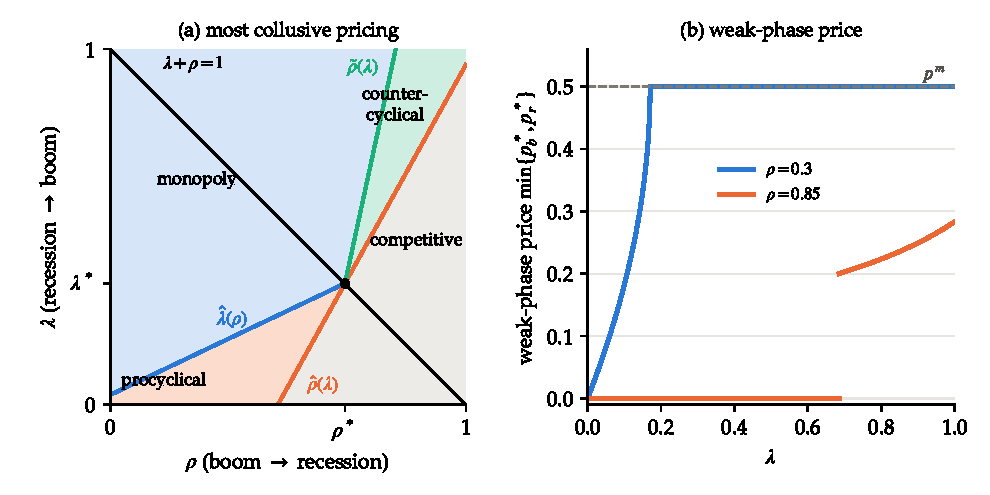
\includegraphics[width=\textwidth]{figures/ch12/bs_regions.pdf}
\caption{Most collusive pricing in the Markov-growth game for $N = 2$, $\delta = 0.9$, $g_b = 1.05$, $g_r = 0.30$,
$\pi(p) = p(1-p)$, $c = 0$. Panel (a): regions in the space of transition probabilities $(\rho, \lambda)$. Below the
anti-diagonal growth rates are positively correlated, above it negatively. The boundaries $\hat\lambda(\rho)$,
$\hat\rho(\lambda)$ and $\tilde\rho(\lambda)$ are \eqref{eq:12-bs-boundaries}, and they meet at $(\rho^*, \lambda^*) \approx (0.659, 0.341)$.
Panel (b): the price in the weak phase as a function of $\lambda$. For $\rho = 0.3$ pricing is procyclical for $\lambda < 0.17$, and
the recession price rises toward $p^m$ as recessions become shorter. For $\rho = 0.85$ pricing is competitive for
$\lambda < 0.686$, then countercyclical with a jump at the boundary. This redraws, with computed regions, Figure 1 of
\citet{BagwellStaiger1995}. Script \texttt{bs\_regions.py}.}
\label{fig:12-bs-regions}
\end{figure}

\subsubsection{Shocks within phases}

The basic model has deterministic demand within a phase. Section V of the paper adds random shocks within phases and
brackets the possibilities with two extremes (WP pp.~24--33). Firms observe the current shock before setting prices.

\casehead{Permanent shocks}
Let $G_t = g_t G_{t-1}\eta_t$, where $\eta_t$ is a multiplicative shock with mean one that becomes part of the base for
all future growth. (Bagwell and Staiger write $\epsilon_t$.) The most
collusive prices depend on the phase but not on the shock. The future is proportional to $G_t$, which already
includes $\eta_t$, so the shock cancels from the incentive constraints, as $G_t$ did before. Formally, the constraints
(WP (22)--(25)) reduce to \eqref{eq:12-bs-ic-b}--\eqref{eq:12-bs-W-r} once $G_t$ is cancelled and $\E[\eta_{t+1}] = 1$ is imposed.
Pricing is exactly as in the basic model (WP Theorem 5).

\casehead{Transitory shocks}
Let $G_t = g_t\frac{G_{t-1}}{\eta_{t-1}}\eta_t$, with $\eta_t$ independent over time, mean one and support $[\underline\eta, \bar\eta]$
containing one. The base level grows without the shock, and the shock affects only the current period. This combines
the Markov phases with Rotemberg-Saloner shocks. Let $p_b(\eta)$ and $p_r(\eta)$ be the prices in each phase when
the current shock is $\eta$. The base level cancels again, but the current shock does not. The boom constraint becomes
(WP (26))
\begin{equation*}
\eta\,\Gamma(p_b(\eta)) \le \delta\left[\rho g_r W_r + (1-\rho)g_b W_b\right],
\end{equation*}
with $W_b$ and $W_r$ defined as before but with $\E[w(p(\eta))\eta]$ in place of $w(p)$ (WP (28)--(29)). The paper solves
the system in two steps, following Rotemberg and Saloner. First it holds the right sides fixed at values
$\tilde W_b$ and $\tilde W_r$. Each constraint then reads $\pi(p_s(\eta)) \le \frac{N}{N-1}\frac{\tilde W_s}{\eta}$ (WP (34)--(35)), and the most
collusive price is
\begin{equation}\label{eq:12-bs-transitory-price}
p_s(\eta) = P^*\!\left(\frac{\tilde W_s}{\eta}\right) \equiv
\begin{cases}
p^m & \text{if } \pi(p^m) \le \frac{N}{N-1}\frac{\tilde W_s}{\eta},\\
\min\left\{p : \pi(p) = \frac{N}{N-1}\frac{\tilde W_s}{\eta}\right\} & \text{otherwise}
\end{cases}
\end{equation}
(WP (36)--(39)). Second, it requires the values $\tilde W_b$ and $\tilde W_r$ to be consistent with the prices they generate
(WP (40)--(43)). It then picks the largest fixed point of the resulting pair of equations. The competitive outcome
$\tilde W_b = \tilde W_r = 0$ is always a fixed point. To leave room for perfect collusion the paper assumes (WP (44))
\begin{equation*}
\delta g_b > \frac{\bar\eta(N-1)}{1 + \bar\eta(N-1)},
\end{equation*}
which says that even the largest shock would not disrupt perfect collusion if growth stayed at the boom rate forever.
To check this, apply the argument of \cref{prop:12-bs-stationary} with current demand scaled by $\bar\eta$:
$\bar\eta(N-1) \le \frac{\delta g_b}{1 - \delta g_b}$ rearranges to the displayed condition.

The results are Theorem 6 of the working paper. Both phases use the same pricing function $P^*$ in
\eqref{eq:12-bs-transitory-price}, and $P^*$ is nondecreasing in $\frac{\tilde W}{\eta}$. So a higher transitory shock lowers the
most collusive price weakly, in booms and in recessions alike. This is the Rotemberg-Saloner effect, now inside each
phase. The comparison between phases still follows the correlation of growth rates. Under positive correlation the
boom value exceeds the recession value at the most collusive fixed point, so $p_b(\eta) \ge p_r(\eta)$ at every shock,
with strict inequality for large shocks. Negative correlation reverses the ranking. The paper's Figures 6a and 6b show
both price schedules flat at $p^m$ for small shocks and falling for large ones. The boom schedule lies above the
recession schedule under positive correlation and below it under negative correlation. Transitory shocks also enlarge
the parameter region with cyclical pricing, because perfect collusion in both phases and at every shock now requires
more. The paper concludes that its second point ``provides an interpretation of the Rotemberg-Saloner (1986) theory in
terms of the transitory demand shocks that occur within broader business-cycle phases'' (WP p.~33).

\subsubsection{Empirical content and limits}

The theory makes the cyclicality of collusive prices an empirical question about the demand process of each industry.
The direction of the cycle depends on the correlation of growth rates, and its amplitude on the expected durations of
booms and recessions. Bagwell and Staiger suggest estimating these parameters industry by industry with Hamilton's
methods and comparing the predictions with industry prices (WP p.~34). No such study existed when they wrote. For
the aggregate economy, \citet{Hamilton1989} finds that quarterly growth rates of U.S. real GNP are positively correlated
and that booms last longer in expectation than recessions. If an industry's demand cycle shares these features, the
prediction of procyclical collusive prices ``appears most salient'' (WP p.~34). Existing evidence points both ways,
and the paper calls it mixed and inconclusive (WP p.~2 and fn.~4). It cites cross-industry studies of margins
\citep{DomowitzHubbardPetersen1986,RotembergWoodford1992}. It cites industry studies, among them
\citet{BorensteinShepard1996}, \citet{Ellison1994}, \citet{Porter1983} and \citet{RotembergSaloner1986}. It also cites
evidence that cartels are most likely to break down during recessions \citep{Suslow1988}.

The authors list three limits (WP pp.~34--35). Marginal costs are acyclic in the model, while the evidence on their
cyclicality is mixed \citep{Bils1987,MironZeldes1988}. Firms are assumed to tell transitory shocks from turning points.
If they observe only demand, they must infer the phase, and the sharp distinction between the responses to the two
kinds of movement will soften. Finally, the analysis is partial equilibrium. With entry and exit the difference between
phases may matter less, and with endogenous interest rates discounting may be more severe in booms.

\subsection{Comparing the models}\label{sec:12-demand-compare}

\Cref{tab:12-cycle-theories} compares the theories of this section with the imperfect-monitoring theory of the next.
The models agree on the logic of the incentive constraint. They disagree on what current demand reveals about the
future and on what firms observe. These two features decide when collusive prices are lowest and whether price wars
appear on the equilibrium path. The table also suggests what data would tell the theories apart. One needs the timing
of low prices relative to the level, growth and predictability of demand. One also needs to know whether low prices
follow observed or unobserved shocks. \Cref{ch:collusion-evidence} takes these predictions to the data.

\begin{table}[htbp]
\centering
\caption{Demand fluctuations and collusive pricing: four theories compared}\label{tab:12-cycle-theories}
\footnotesize
\begin{tabularx}{\textwidth}{@{}>{\raggedright\arraybackslash}p{2.35cm}>{\raggedright\arraybackslash}X>{\raggedright\arraybackslash}X>{\raggedright\arraybackslash}p{2.2cm}>{\raggedright\arraybackslash}X@{}}
\toprule
Model & What drives the future loss & When collusive prices are lowest & Price wars on the path? & Testable implication\\
\midrule
\citet{RotembergSaloner1986}: observed independent shocks & Expected demand, the same in every state & In high-demand states, above a cutoff & No (yes only with collude-or-compete strategies) & Margins fall when current demand is high\\[3pt]
\citet{HaltiwangerHarrington1991}: deterministic cycle & Demand along the known future path & When demand is about to fall, and at the peak for impatient firms & No & At equal demand, prices higher when demand rises than when it falls\\[3pt]
\citet{BagwellStaiger1997}: Markov growth phases & Expected future growth, which depends on the phase & In recessions under positive correlation, in booms under negative correlation & No & Direction and amplitude of the price cycle depend on correlation and phase durations\\[3pt]
\citet{GreenPorter1984}: unobserved shocks (\cref{sec:12-public}) & Probability that a low price triggers a war & After unexpectedly low demand & Yes, finite reversions & Wars follow negative demand shocks and are not caused by cheating\\
\bottomrule
\end{tabularx}
\end{table}

\section{Imperfect Public Monitoring: Green and Porter}\label{sec:12-public}

In the models of \cref{sec:12-perfect,sec:12-demand}, every firm sees every rival's price. A deviation is detected
at once, the threat of punishment deters it, and punishments are never carried out. Prices on the equilibrium path
may move with demand, but no price war is ever triggered by a suspicion of cheating. This section removes perfect
observability. Firms now see only a signal that depends both on their rivals' actions and on demand shocks that
nobody observes. When all firms see the same signal, we speak of \emph{imperfect public monitoring}. The signal is
an imperfect indicator of conduct, so a cartel cannot condition punishments on deviations. It must condition them on
outcomes, and outcomes are sometimes bad even when nobody cheats.

The consequence is the central result of this section. Price wars occur on the equilibrium path, and they are
necessary to sustain collusion. We first recall the policing problem of \citet{Stigler1964}, which motivated the
theory. We then study a Bertrand version that conveys the logic in a few lines, and the original Cournot model of
\citet{GreenPorter1984}. The section ends with the stochastic process of prices that the model generates, which is
the basis for the empirical tests of \cref{sec:13-jec}.

\subsection{Secret price cuts: Stigler's policing problem}\label{sec:12-stigler-recap}

\citet{Stigler1964} accepted that oligopolists wish to maximize joint profits and asked why they so often fail.
His answer is that a collusive agreement must be policed, and that policing is a problem of information. Any member
who can cut its price secretly earns more than by conforming. Enforcement therefore consists of detecting
significant deviations. Once a cut is detected, rivals match it, so it stops paying. The difficulty is detection
itself. Transaction prices are private, buyers have an interest in reporting fictitious offers, and a price cut can
be disguised in non-price terms of the sale. Stigler concluded that the basic evidence of a price cut is that the
cutter wins business it would otherwise not obtain \citep[Section II]{Stigler1964}. His definition of perfect
collusion is accordingly that no buyer changes sellers voluntarily.

This view yields testable implications, which \cref{sec:02-stigler} develops with Stigler's statistical model and
evidence. Suppose each cut offered to a single buyer reaches a rival with probability $h$. A cut offered to $n$
buyers is then detected with probability $1 - (1 - h)^n$, which approaches one quickly as $n$ grows. Secret cuts
are therefore offered to large buyers, and collusion holds best against many small ones. Public sealed-bid
purchases reveal prices and make collusion easier. Collusion is harder when the identity of buyers changes often,
because a seller's loss of customers is then a noisy signal. The incentive to cut prices secretly grows roughly in
proportion to the number of rivals, so collusion is harder with more sellers. The variance of firms' sales to new
customers depends on the Herfindahl index, which makes it the natural measure of concentration for this problem.

Stigler's account has a gap that the rest of this section fills. It takes for granted that detected cuts are
punished, and it offers no equilibrium theory of punishment when detection is noisy. In his account a price war is
the sign that a cartel has broken down. \citet{GreenPorter1984} read Stigler differently. They treat the cartel as
the solution of a design problem: an institution whose members behave noncooperatively and whose incentives must be
self-enforcing. With noisy signals, the best such institution must sometimes punish members who did not cheat.

\subsection{A Bertrand version with zero-demand shocks}\label{sec:12-gp-bertrand}

The logic of on-path price wars is clearest in a price-setting model with a very simple form of noise. This version
is the textbook simplification of \citet[section~6.7.1.1]{Tirole1988} of the Cournot model of
\citet{GreenPorter1984}, which we study in \cref{sec:12-gp-original}. Tirole replaces quantity competition by price
competition so that firms infer rivals' prices from their own demand, as \citet{Stigler1964} assumed. He writes
$\alpha$ for the probability of zero demand, which we call $\gamma$. His section~6.7.1 on secret price cuts, which
also treats quantity competition, spans pp.~262--265 of the print edition \citep[p.~16, note~27]{MarshallMarx2012}.

\needspace{6\baselineskip}
\begin{assumption}[Bertrand duopoly with unobserved demand shocks]\label{asm:12-gp-bertrand}
\leavevmode
\begin{enumerate}[label=(\roman*)]
\item Two firms sell a homogeneous good at constant marginal cost $c$. They set prices simultaneously in each period
$t = 0, 1, 2, \dots$ and discount the future with the factor $\delta \in (0,1)$.
\item In each period demand is $D(p)$ with probability $1 - \gamma$ and zero with probability $\gamma \in (0,1)$,
independently over time. The state is drawn after prices are set, and no firm ever observes it.
\item Industry profit $\pi(p) = (p - c)D(p)$ is continuous and has a unique maximizer $p^m$, with
$\pi^m \equiv \pi(p^m) > 0$.
\item Each firm observes its own price and its own sales. It never observes the rival's price or the state.
\end{enumerate}
\end{assumption}

The lowest price serves the market and ties are split equally. Firm $i$'s sales when the rival charges $p_j$ are
therefore
\begin{equation}\label{eq:12-gp-sales}
q_i =
\begin{cases}
D(p_i) & \text{if } p_i < p_j \text{ and demand is } D(\cdot),\\[2pt]
\frac{1}{2}D(p_i) & \text{if } p_i = p_j \text{ and demand is } D(\cdot),\\[2pt]
0 & \text{if } p_i > p_j \text{ or demand is zero.}
\end{cases}
\end{equation}
The model builds Stigler's inference problem into the payoffs. A firm that charged $p^m$ and sold nothing cannot tell
whether demand was zero or its rival undercut it. Its only signal is its own sales, and zero sales are consistent
with both events.

\begin{definition}[Trigger strategy with punishment length $T$]\label{def:12-gp-trigger}
Fix an integer $T \ge 1$. Each period is either collusive or a punishment period, and period $0$ is collusive. In a
collusive period the firm charges $p^m$. Suppose that in a collusive period the firm's own sales are zero, or the
firm itself charged a price different from $p^m$. Then the next $T$ periods are punishment periods, in which the firm
charges $c$. The period after the last punishment period is collusive. In every other case a collusive period is followed by
a collusive period.
\end{definition}

When both firms follow this strategy, both charge $p^m$ in collusive periods. Both then sell nothing exactly when
demand is zero, so their phases always coincide. Every zero-demand period in a collusive phase starts a \emph{price
war} of $T$ periods at marginal cost, although nobody has cheated. We say that such a war is on the
\emph{equilibrium path}.

\begin{proposition}[Collusion with a finite price war]\label{prop:12-gp-bertrand}
Under \cref{asm:12-gp-bertrand}, the value of a firm at the start of a collusive period when both firms follow the
trigger strategy of \cref{def:12-gp-trigger} is
\begin{equation}\label{eq:12-gp-V}
V = \frac{(1 - \gamma)\frac{\pi^m}{2}}{1 - (1 - \gamma)\delta - \gamma\delta^{T + 1}} .
\end{equation}
The trigger profile is a Nash equilibrium if and only if
\begin{equation}\label{eq:12-gp-ic}
\Lambda(T) \equiv 2(1 - \gamma)\delta + (2\gamma - 1)\delta^{T + 1} \;\ge\; 1 .
\end{equation}
\end{proposition}

\begin{proof}
\emph{Value of collusion.} Consider a collusive period. With probability $1 - \gamma$ demand is positive, each firm
sells $\frac{1}{2}D(p^m)$ and earns $\frac{\pi^m}{2}$, and the next period is collusive. With probability $\gamma$
demand is zero, each firm earns zero, and a war fills periods $t + 1$ to $t + T$. Profits in the war are zero, and
collusion resumes in period $t + T + 1$, whose value seen from period $t$ is $\delta^{T + 1}V$. Hence
\begin{equation*}
V = (1 - \gamma)\Bigl(\frac{\pi^m}{2} + \delta V\Bigr) + \gamma\,\delta^{T + 1}V .
\end{equation*}
Collect the terms in $V$:
\begin{equation*}
V\bigl[1 - (1 - \gamma)\delta - \gamma\delta^{T + 1}\bigr] = (1 - \gamma)\frac{\pi^m}{2} .
\end{equation*}
The bracket is positive because $(1 - \gamma)\delta + \gamma\delta^{T + 1} < 1$. Dividing gives \eqref{eq:12-gp-V}.

\emph{Deviations in a war.} In a punishment period the rival charges $c$. Any price earns at most zero, so charging
$c$ is a best response, and the firm's price cannot change the length of the war. Only deviations in collusive
periods need to be checked.

\emph{Deviations in a collusive period.} A price above $p^m$ earns zero today. It leaves the rival's next phase
exactly as under conformity: the rival sells something when demand is positive and nothing otherwise. It is
therefore dominated by charging $p^m$. A price $p < p^m$ wins the whole market when demand is positive and earns
$(1 - \gamma)(p - c)D(p) \le (1 - \gamma)\pi^m$ in expectation. The rival then sells nothing whatever the state, so
a war starts for sure. The supremum of the current gain, $(1 - \gamma)\pi^m$, is approached as $p \uparrow p^m$.

\emph{Best responses.} Give firm $i$ the extra information of the rival's current phase, which can only raise its
best payoff. Let $W$ be the supremum of $i$'s payoff at the start of a rival's collusive phase. In a war the firm
earns at most zero per period, and the rival returns to collusion after $T$ periods whatever $i$ does. Dynamic
programming then gives
\begin{equation*}
W = \max\Bigl\{(1 - \gamma)\frac{\pi^m}{2} + \bigl[(1 - \gamma)\delta + \gamma\delta^{T + 1}\bigr]W,\;\;
(1 - \gamma)\pi^m + \delta^{T + 1}W\Bigr\}.
\end{equation*}
The right side is a contraction in $W$, so $W$ is its unique bounded fixed point. Define the value of the best
one-shot undercut as
\begin{equation*}
V^d \equiv (1 - \gamma)\pi^m + \delta^{T + 1}V .
\end{equation*}
If $V \ge V^d$, then $V$ solves the fixed-point equation, because the first branch equals $V$ by the recursion
above. Hence $W = V$, and conformity is a best response. If $V < V^d$, an undercut close to $p^m$ followed by the
trigger strategy is a profitable deviation. The profile is therefore an equilibrium if and only if $V \ge V^d$.

\emph{The condition.} Replace $V$ on the left of $V \ge V^d$ by its recursion:
\begin{equation*}
(1 - \gamma)\frac{\pi^m}{2} + \bigl[(1 - \gamma)\delta + \gamma\delta^{T + 1}\bigr]V \;\ge\; (1 - \gamma)\pi^m + \delta^{T + 1}V .
\end{equation*}
Move the terms in $V$ to the left and the others to the right:
\begin{equation*}
\bigl[(1 - \gamma)\delta - (1 - \gamma)\delta^{T + 1}\bigr]V \;\ge\; (1 - \gamma)\frac{\pi^m}{2} .
\end{equation*}
Divide by $1 - \gamma$:
\begin{equation}\label{eq:12-gp-ic-V}
\bigl(\delta - \delta^{T + 1}\bigr)V \;\ge\; \frac{\pi^m}{2} .
\end{equation}
Substitute \eqref{eq:12-gp-V} and cancel $\frac{\pi^m}{2}$:
\begin{equation*}
(1 - \gamma)\bigl(\delta - \delta^{T + 1}\bigr) \;\ge\; 1 - (1 - \gamma)\delta - \gamma\delta^{T + 1} .
\end{equation*}
Collect terms:
\begin{equation*}
2(1 - \gamma)\delta - (1 - \gamma)\delta^{T + 1} + \gamma\delta^{T + 1} \;\ge\; 1 ,
\end{equation*}
which is \eqref{eq:12-gp-ic}.
\end{proof}

The proposition reproduces Tirole's equations (6.10) to (6.16) in our notation. His (6.10) and (6.11) are the
recursions for the values of the collusive and punishment phases, with $V^- = \delta^TV^+$. His (6.14) is
\eqref{eq:12-gp-V}, his incentive constraint (6.13), $\delta(V^+ - V^-) \ge \frac{\pi^m}{2}$, is
\eqref{eq:12-gp-ic-V}, and his (6.16) is \eqref{eq:12-gp-ic} exactly.

Condition \eqref{eq:12-gp-ic-V} has a simple reading. An undercut raises current profit by $\frac{\pi^m}{2}$ when
demand is positive. Its cost is that a war then starts for sure rather than with probability $\gamma$. The extra
probability of a war is $1 - \gamma$, and a war destroys the $T$ collusive periods that would have followed, worth
$(\delta - \delta^{T + 1})V$. Both the gain and the extra probability carry the factor $1 - \gamma$, which cancels.
Two special cases connect the result to earlier sections. With an infinite war ($T = \infty$), $\delta^{T + 1} = 0$
and the condition becomes $\delta(1 - \gamma) \ge \frac{1}{2}$. Without noise ($\gamma = 0$) the condition becomes
$2\delta - \delta^{T + 1} \ge 1$, which is equivalent to $\delta + \delta^2 + \dots + \delta^T \ge 1$. A long enough
punishment works if and only if $\delta > \frac{1}{2}$, and permanent reversion works if and only if
$\delta \ge \frac{1}{2}$. This is the duopoly threshold $1 - \frac{1}{N}$ of \cref{prop:12-bertrand}.

\begin{corollary}[The optimal length of a price war]\label{cor:12-gp-optimal-T}
Under \cref{asm:12-gp-bertrand}:
\begin{enumerate}[label=(\roman*)]
\item $V$ is strictly decreasing in $T$ and in $\gamma$.
\item If $\gamma \ge \frac{1}{2}$, no $T$ satisfies \eqref{eq:12-gp-ic}. If $\gamma < \frac{1}{2}$, the function
$\Lambda(T)$ is strictly increasing in $T$, with $\Lambda(0) = \delta$ and $\lim_{T \to \infty} \Lambda(T) = 2(1 - \gamma)\delta$.
Some finite $T$ satisfies \eqref{eq:12-gp-ic} if and only if $2(1 - \gamma)\delta > 1$.
\item The most profitable trigger equilibrium uses the shortest war that satisfies \eqref{eq:12-gp-ic},
\begin{equation}\label{eq:12-gp-Tstar}
T^* = \min\Bigl\{T \ge 1 : \delta^{T + 1} \le x\Bigr\},
\qquad
x \equiv \frac{2(1 - \gamma)\delta - 1}{1 - 2\gamma} .
\end{equation}
\item The threshold $\frac{1}{2(1 - \gamma)}$ that $\delta$ must exceed rises with $\gamma$, and $T^*$ is weakly
increasing in $\gamma$.
\item A war of one period never suffices: $\Lambda(1) < 1$ for every $\gamma \in [0, 1)$ and $\delta \in (0, 1)$, so
$T^* \ge 2$ whenever collusion is sustainable.
\end{enumerate}
\end{corollary}

\begin{proof}
(i) Write the denominator of \eqref{eq:12-gp-V} as $1 - \delta + \gamma(\delta - \delta^{T + 1})$. It rises with
$T$ because $\delta^{T + 1}$ falls, and it rises with $\gamma$. The numerator falls with $\gamma$. (ii) If
$\gamma \ge \frac{1}{2}$, then $2\gamma - 1 \ge 0$ and $\delta^{T + 1} \le \delta$, so
$\Lambda(T) \le 2(1 - \gamma)\delta + (2\gamma - 1)\delta = \delta < 1$. If $\gamma < \frac{1}{2}$, the coefficient
$2\gamma - 1$ is negative and $\delta^{T + 1}$ falls with $T$, so $\Lambda$ rises toward its limit. (iii) By (i) the
cartel prefers the shortest admissible war. With $\gamma < \frac{1}{2}$, condition \eqref{eq:12-gp-ic} is
equivalent to $(1 - 2\gamma)\delta^{T + 1} \le 2(1 - \gamma)\delta - 1$, that is, to $\delta^{T + 1} \le x$.
(iv) The derivative of $x$ with respect to $\gamma$ is
\begin{equation*}
\frac{\partial x}{\partial \gamma} = \frac{-2\delta(1 - 2\gamma) + 2\bigl[2(1 - \gamma)\delta - 1\bigr]}{(1 - 2\gamma)^2}
= \frac{2(\delta - 1)}{(1 - 2\gamma)^2} < 0 .
\end{equation*}
A smaller $x$ requires a larger $T + 1$, so $T^*$ cannot fall when $\gamma$ rises. (v) Evaluate $\Lambda$ at $T = 1$
and subtract one:
\begin{align*}
\Lambda(1) - 1 &= 2(1 - \gamma)\delta + (2\gamma - 1)\delta^2 - 1 \\
&= -\bigl(1 - 2\delta + \delta^2\bigr) - 2\gamma\delta(1 - \delta) \\
&= -(1 - \delta)\bigl[(1 - \delta) + 2\gamma\delta\bigr] \;<\; 0 .
\end{align*}
Since $\Lambda(0) = \delta < 1$ as well, no war shorter than two periods satisfies \eqref{eq:12-gp-ic}.
\end{proof}

Part (v) is the second half of Tirole's Exercise~6.8, which sets $\gamma = \frac{1}{4}$. Collusion then needs
$\delta > \frac{1}{2(1 - \frac{1}{4})} = \frac{2}{3}$, and at least two punishment periods are required. The result
holds for every $\gamma$. It explains why neither \cref{ex:12-gp-numbers} below nor Exercise~5 of
\cref{sec:12-exercises} can have $T^* = 1$. With their parameters a war of two periods already satisfies
\eqref{eq:12-gp-ic}, so $T^* = 2$ in both. The reason is visible in the case $\gamma = 0$. A one-period war costs the deviator its share
$\frac{\pi^m}{2}$ one period later, worth $\delta\frac{\pi^m}{2}$, while undercutting gains $\frac{\pi^m}{2}$ today. The
loss falls short of the gain for every $\delta < 1$, and noise only widens the gap.

The trade-off behind \cref{cor:12-gp-optimal-T} is specific to imperfect monitoring. Under perfect monitoring a
harsher punishment is free, because it is never used. Here every war is fought on the path, so a longer war lowers
the value of collusion directly. The war must be long enough to deter undercutting and no longer. A war of length
zero or one never works, by part (v). Noise of one half or more makes collusion impossible with these strategies.
A firm that conforms then triggers a war more often than not, and a deviation raises the probability of war too
little to deter it.

The long-run frequency of wars follows from a Markov chain with states ``collusive'' and ``war, $k$ periods
elapsed'' for $k = 1, \dots, T$. Let $\psi_0$ be the stationary probability of a collusive period. A collusive period
leads to a war with probability $\gamma$, and every war lasts $T$ periods, so each war state has stationary
probability $\gamma\psi_0$. The probabilities sum to one, $\psi_0(1 + \gamma T) = 1$, and the long-run share of
periods spent in wars is
\begin{equation}\label{eq:12-gp-war-share}
1 - \psi_0 = \frac{\gamma T}{1 + \gamma T} .
\end{equation}
Collusive spells last $\frac{1}{\gamma}$ periods on average, counting the period that triggers the war.

\begin{example}[Numbers]\label{ex:12-gp-numbers}
Let $\delta = 0.9$ and $\gamma = 0.1$. The limit of $\Lambda(T)$ is $2(0.9)(0.9) = 1.62 > 1$, so collusion is
sustainable. Condition \eqref{eq:12-gp-ic} reads $1.62 - 0.8(0.9)^{T + 1} \ge 1$, that is,
$0.9^{T + 1} \le \frac{0.62}{0.8} = 0.775$. Since $\frac{\ln 0.775}{\ln 0.9} = 2.42$, we need $T + 1 \ge 3$. A war of
one period fails ($0.9^2 = 0.81$), and a war of two periods works ($0.9^3 = 0.729$), so $T^* = 2$. By
\eqref{eq:12-gp-V}, $V = \frac{0.45}{1 - 0.81 - 0.0729}\pi^m = 3.84\,\pi^m$. The same strategies with an infinite war
give $V = \frac{0.45}{0.19}\pi^m = 2.37\,\pi^m$, and perfect monitoring gives $\frac{0.5}{0.1}\pi^m = 5\,\pi^m$. By
\eqref{eq:12-gp-war-share}, the firms spend $\frac{0.2}{1.2} = \frac{1}{6}$ of all periods in wars. All numbers are
computed by \texttt{figures/ch12/src/gp\_path.py}.
\end{example}

\begin{figure}[htbp]
\centering
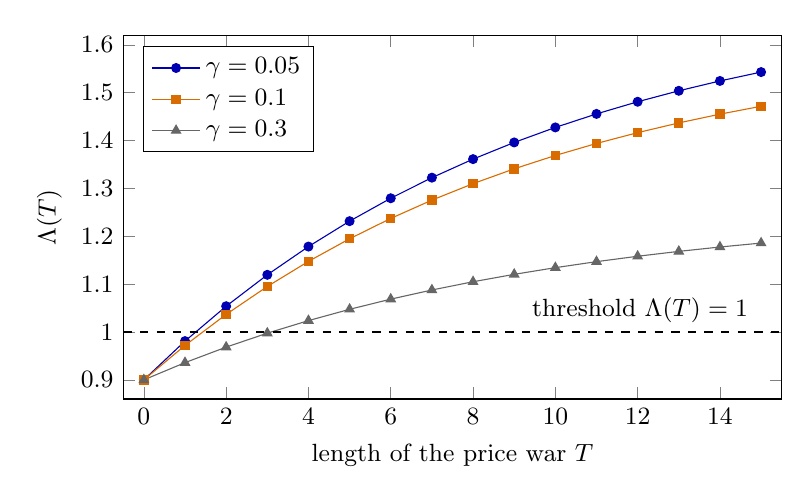
\begin{tikzpicture}
\begin{axis}[
  width=0.82\textwidth, height=6.2cm,
  xlabel={length of the price war $T$}, ylabel={$\Lambda(T)$},
  xmin=-0.5, xmax=15.5, ymin=0.86, ymax=1.62,
  xtick={0,2,4,6,8,10,12,14}, ytick={0.9,1.0,1.1,1.2,1.3,1.4,1.5,1.6},
  legend pos=north west, legend cell align=left,
  tick label style={font=\small}, label style={font=\small}, legend style={font=\small}]
\addplot[blue!70!black, mark=*, mark size=1.6pt, domain=0:15, samples=16]
  {2*(1-0.05)*0.9 + (2*0.05-1)*0.9^(x+1)};
\addlegendentry{$\gamma = 0.05$}
\addplot[orange!85!black, mark=square*, mark size=1.5pt, domain=0:15, samples=16]
  {2*(1-0.1)*0.9 + (2*0.1-1)*0.9^(x+1)};
\addlegendentry{$\gamma = 0.1$}
\addplot[gray!80!black, mark=triangle*, mark size=1.9pt, domain=0:15, samples=16]
  {2*(1-0.3)*0.9 + (2*0.3-1)*0.9^(x+1)};
\addlegendentry{$\gamma = 0.3$}
\addplot[black, dashed, domain=-0.5:15.5, samples=2, forget plot] {1};
\node[font=\small, anchor=south west] at (axis cs:9.2,1.0) {threshold $\Lambda(T) = 1$};
\end{axis}
\end{tikzpicture}
\caption{The left side of the incentive constraint \eqref{eq:12-gp-ic} as a function of the length of the price war,
for $\delta = 0.9$. Collusion is sustainable with punishment length $T$ when $\Lambda(T) \ge 1$. The shortest admissible war
is $T^* = 2$ for $\gamma = 0.05$ and $\gamma = 0.1$, and $T^* = 4$ for $\gamma = 0.3$. The curves approach
$2(1 - \gamma)\delta$ as $T$ grows.}\label{fig:12-gp-ic}
\end{figure}

\begin{figure}[htbp]
\centering
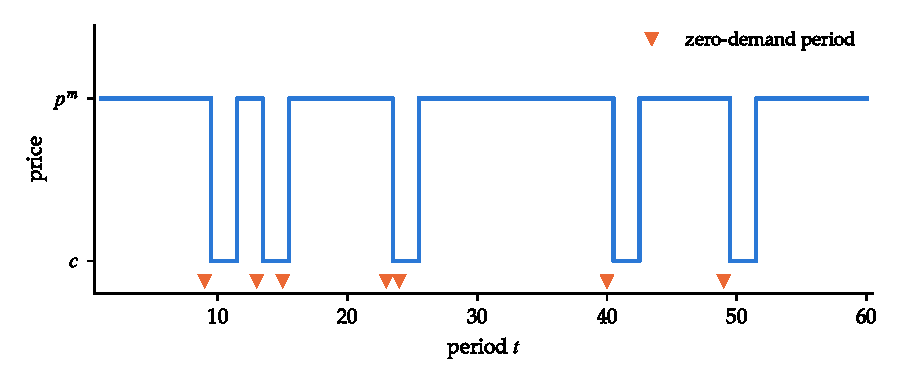
\includegraphics[width=0.92\textwidth]{figures/ch12/gp_path.pdf}
\caption{A simulated equilibrium price path in the Bertrand version of Green and Porter, with $\gamma = 0.1$ and the
optimal war length $T = 2$ for $\delta = 0.9$. Triangles mark periods of zero demand. A zero-demand period in a
collusive phase starts a two-period war at marginal cost. Zero-demand periods inside a war (periods 15 and 24) have
no effect. Wars occupy 10 of the 60 periods, the long-run share $\frac{1}{6}$. Nobody ever cheats. Source: our
simulation, \texttt{figures/ch12/src/gp\_path.py}.}\label{fig:12-gp-path}
\end{figure}

\Cref{fig:12-gp-ic,fig:12-gp-path} summarize four lessons. First, price wars occur on the equilibrium path even
though no firm ever cuts its price. They are necessary: if firms forgave zero sales, undercutting would go
unpunished and collusion would unravel. Second, optimal collusion uses a finite war, as short as the incentive
constraint allows. Third, more noise makes collusion harder. The patience required rises with $\gamma$, and both the
expected collusive profit and the value of collusion fall. Fourth, wars follow unexpectedly low demand. This timing
is the opposite of \cref{sec:12-rs}, where demand is observed and collusive prices are lowest in booms.
\Cref{tab:12-cycle-theories} compares the predictions, and \cref{sec:13-jec} confronts them with data.

The equilibrium has an uncomfortable feature. When a war starts, both firms know that nobody cheated, since each
knows the other's strategy. Both would gain by skipping the war, yet the war is needed to keep conformity optimal in
collusive periods. Equilibria of this kind are not robust to renegotiation after bad outcomes. Cartels that can talk
and audit each other's sales can avoid some of these wars, which is one reason why explicit cartels organize
monitoring (\cref{sec:12-cartels}).

\casehead{N firms, random punishments and the value of transparency}
\Citet[pp.~203--205]{AskerNocke2021} use a variant of this model with $N$ firms and a noisy public signal. It yields
closed forms for the threshold and for the value of collusion, and it shows why transparency matters even far above
the threshold. We state it in our notation. Asker and Nocke write $n$ for $N$, $\beta$ for our $\gamma$, $\alpha$ for
our $\lambda$ and $\rho$ for our $\phi$, and their $\pi^m$ is our expected profit $\bar\pi$.

\begin{assumption}[Bertrand oligopoly with a noisy public signal]\label{asm:12-an}
\leavevmode
\begin{enumerate}[label=(\roman*)]
\item $N$ identical firms sell a homogeneous good at marginal cost $c$. Demand in period $t$ is $\theta_tD(p)$, where
$\theta_t = 0$ with probability $\gamma$ and $\theta_t = 1$ otherwise, independently over time. Write
$\bar\pi = (1 - \gamma)\pi^m$ for the expected monopoly profit.
\item Firms observe neither $\theta_t$ nor rivals' prices. At the start of period $t$ they observe a public signal
$s_t \in \{0, 1\}$. It equals one if some firm priced below $p^m$ in period $t - 1$. If all firms charged at least
$p^m$, it equals one with probability $\lambda$ when $\theta_{t-1} = 0$ and zero otherwise.
\item A public random variable $r_t$, uniform on $[0, 1]$, is drawn at the start of each period. The signal is noisy,
$\gamma\lambda > 0$, and satisfies $\gamma\lambda < \frac{1}{N}$.
\end{enumerate}
\end{assumption}

Under the strategy profile $\sigma(\phi)$, every firm charges $p^m$ until the first period in which $s_t = 1$ and
$r_t \le \phi$. From then on every firm prices at $c$ forever. A bad signal thus triggers Nash reversion with
probability $\phi \in [0, 1]$, and the cartel chooses $\phi$. The profile conditions only on public information. It is
a \emph{perfect public equilibrium} if it is optimal for every firm after every public history.
\Cref{sec:12-abs-repeated} gives the formal definition.

\begin{proposition}[Threshold and value with a noisy signal]\label{prop:12-an}
Under \cref{asm:12-an}, $\sigma(\phi)$ is a perfect public equilibrium if and only if
\begin{equation}\label{eq:12-an-phi}
\phi \;\ge\; \phi^* \equiv \frac{1 - \delta}{\delta}\cdot\frac{N - 1}{1 - N\gamma\lambda} .
\end{equation}
Collusion at $p^m$ is therefore sustainable in this class if and only if
\begin{equation}\label{eq:12-an-delta}
\delta \;\ge\; \underline\delta = \frac{N - 1}{N(1 - \gamma\lambda)} .
\end{equation}
The best such equilibrium uses $\phi^*$, and each firm's per-period value is
\begin{equation}\label{eq:12-an-value}
v^* = (1 - \delta)V(\phi^*) = \frac{1 - N\gamma\lambda}{1 - \gamma\lambda}\cdot\frac{\bar\pi}{N} .
\end{equation}
\end{proposition}

\begin{proof}
On the path, each firm earns $\frac{\bar\pi}{N}$ in expectation. Reversion is triggered next period with probability
$\gamma\lambda\phi$, after which every firm earns zero. The value before reversion therefore solves
\begin{equation*}
V(\phi) = \frac{\bar\pi}{N} + \delta(1 - \gamma\lambda\phi)V(\phi)
\quad\Longrightarrow\quad
V(\phi) = \frac{\bar\pi}{N\bigl[1 - \delta(1 - \gamma\lambda\phi)\bigr]} .
\end{equation*}
A firm that undercuts slightly earns almost $\bar\pi$ in expectation, and the signal then equals one for sure.
Reversion follows with probability $\phi$, so the best one-shot deviation is worth
$V^{\mathrm{dev}}(\phi) = \bar\pi + \delta(1 - \phi)V(\phi)$. Reversion is a stage equilibrium after every history,
so by the one-shot deviation principle the profile is an equilibrium if and only if $V(\phi) \ge V^{\mathrm{dev}}(\phi)$.
Rearrange this as $V(\phi)\bigl[1 - \delta(1 - \phi)\bigr] \ge \bar\pi$ and substitute $V(\phi)$:
\begin{equation*}
\frac{1 - \delta + \delta\phi}{N\bigl[1 - \delta + \delta\gamma\lambda\phi\bigr]} \ge 1
\quad\Longleftrightarrow\quad
1 - \delta + \delta\phi \ge N(1 - \delta) + N\delta\gamma\lambda\phi .
\end{equation*}
Collect the terms in $\phi$:
\begin{equation*}
\delta\phi\,(1 - N\gamma\lambda) \;\ge\; (N - 1)(1 - \delta) .
\end{equation*}
Since $N\gamma\lambda < 1$, dividing gives \eqref{eq:12-an-phi}. A probability $\phi \le 1$ satisfies it if and only
if $\phi^* \le 1$, that is, $\delta(1 - N\gamma\lambda) \ge (N - 1)(1 - \delta)$. Collecting the terms in $\delta$ gives
$\delta(N - N\gamma\lambda) \ge N - 1$, which is \eqref{eq:12-an-delta}. The value $V(\phi)$ falls with $\phi$, so the
best equilibrium in the class uses $\phi^*$. At $\phi^*$,
\begin{equation*}
\delta\gamma\lambda\phi^* = \frac{(1 - \delta)(N - 1)\gamma\lambda}{1 - N\gamma\lambda},
\qquad
1 - \delta + \delta\gamma\lambda\phi^* = (1 - \delta)\,\frac{1 - \gamma\lambda}{1 - N\gamma\lambda} .
\end{equation*}
Substituting into $(1 - \delta)V(\phi^*)$ gives \eqref{eq:12-an-value}.
\end{proof}

These are equations (3) to (5) of Asker and Nocke. Two special cases connect them with the rest of the chapter. With
perfect monitoring, $\lambda = 0$, the threshold is $\frac{N - 1}{N}$ of \cref{prop:12-bertrand} and $v^* =
\frac{\bar\pi}{N}$. With $N = 2$ and $\lambda = 1$, zero demand always triggers the signal, as zero sales do in
\cref{asm:12-gp-bertrand}. The threshold \eqref{eq:12-an-delta} is then $\frac{1}{2(1 - \gamma)}$, the threshold of
\cref{cor:12-gp-optimal-T} for an infinite war.

The result changes how we should read comparative statics. Under perfect monitoring the per-period value jumps from
zero to $\frac{\bar\pi}{N}$ at the threshold and is flat above it. A small change in the number of firms then has no
effect on collusion unless $\delta$ is close to the threshold. With noise, $v^*$ falls continuously with $N$ and with
$\gamma\lambda$ however patient the firms are \citep[p.~205]{AskerNocke2021}. Better observability of deviations, a
lower $\lambda$, lowers the threshold and also raises $v^*$, because the cartel can punish less often on the path.
Take $N = 3$ and $\gamma = 0.2$, our own illustration. With $\lambda = 0.5$ the threshold is
$\frac{2}{3(0.9)} \approx 0.741$ and $v^*$ is $\frac{0.7}{0.9} \approx 0.78$ of the perfect-monitoring value. With
$\lambda = 0.25$ these become $\frac{2}{3(0.95)} \approx 0.702$ and $\frac{0.85}{0.95} \approx 0.89$. This is the
formal content of the view that transparent prices facilitate collusion. \citet{SugayaWolitzky2018} point out a
limit. Some information lets a firm tailor its deviation to current conditions. A cartel member that learns in advance
that its cost of serving a rival's territory is low can deviate exactly then, which makes collusion harder
\citep[p.~205, note~69]{AskerNocke2021}.

\subsection{The original model: Green and Porter (1984)}\label{sec:12-gp-original}

\casehead{Question and context}
\citet{GreenPorter1984} ask how a cartel can enforce collusion when firms cannot observe each other's outputs and
demand is uncertain. Two rigorous formulations of noncooperative collusion existed. In the reaction-function
equilibrium of \citet{Osborne1976}, firms respond to output changes so as to keep their shares. In the supergame of
\citet{Friedman1971}, firms revert to Cournot behavior forever after a price drop. In both, incentives are so perfect
that deterrence is never observed. Time-series data then cannot tell a collusive equilibrium from a competitive one
\citep{Bresnahan1982}. Green and Porter show that this perfection is an artifact of certainty. With imperfect
information, optimal incentive schemes involve recurrent episodes of the conduct previously called price wars or
punishments (pp.~87--88).

\casehead{Which industries the model describes}
The authors list four structural features of a suitable industry (p.~90). First, the industry is stable over time,
which makes rational expectations credible and justifies stationary dynamic programming. Second, output is the only
decision variable. Firms cannot differentiate products or divide the market, so a suspected cheater cannot be
isolated and punished alone. Third, all information except each firm's own output is public. Firms know each other's
cost functions, and all observe a common variable that tells them whether the industry is in a collusive or a
reversionary state. Fourth, this monitoring variable is imperfectly correlated with conduct. Otherwise reversions
would never occur. The fourth feature excludes markets with few, publicly announced transactions, such as contracts
awarded by sealed bids. The authors propose the American rail freight industry of the 1880s as an example
(p.~94), the cartel analyzed by \citet{Porter1983} in \cref{sec:13-jec}.

\begin{assumption}[The Green-Porter environment]\label{asm:12-gp}
\leavevmode
\begin{enumerate}[label=(\roman*)]
\item There are $N$ firms producing a homogeneous good. Firm $i$'s net return from producing $x_i$ units and selling
at price $p$ is $\pi_i(x_i, p)$. Firms are risk neutral and maximize $\E\bigl[\sum_{t \ge 0}\delta^t\pi_i(x_{it}, p_t)\bigr]$.
\item The observed price is
\begin{equation}\label{eq:12-gp-price}
p_t = \eta_t\,P\Bigl(\sum_{i=1}^N x_{it}\Bigr),
\end{equation}
where $P$ is a decreasing inverse demand function and the shocks $\eta_t$ are \iid\ with cdf $F_\eta$, continuous
density $f_\eta$, and $\E[\eta_t] = 1$. No firm observes $\eta_t$.
\item Each firm observes the history of prices and its own outputs. It never observes its rivals' outputs.
\end{enumerate}
\end{assumption}

We change the paper's notation. Its discount factor $\beta$ is our $\delta$, and its inverse demand $p(\cdot)$ is our
$P(\cdot)$. Its demand shock $\theta_t$ is our $\eta_t$, since $\theta$ is the conduct parameter in this book. A
\emph{contingent strategy} for firm $i$ is a sequence $s_i = (s_{i0}, s_{i1}, \dots)$, where $s_{i0}$ is an initial
output and $s_{i,t+1}(p_0, \dots, p_t)$ gives the output at $t + 1$ as a function of past prices. Write $\E_{s}$ for
the expectation under the price process generated by a profile $s$. A \emph{Nash equilibrium} is a profile
$s^* = (s_1^*, \dots, s_N^*)$ such that, for every firm $i$ and every feasible $s_i$ (GP (1), p.~91),
\begin{equation}\label{eq:12-gp-nash}
\E_{s_1^*, \dots, s_i, \dots, s_N^*}\Biggl[\sum_{t = 0}^{\infty}\delta^t\pi_i\bigl(s_{it}(p_0, \dots, p_{t-1}), p_t\bigr)\Biggr]
\;\le\;
\E_{s^*}\Biggl[\sum_{t = 0}^{\infty}\delta^t\pi_i\bigl(s_{it}^*(p_0, \dots, p_{t-1}), p_t\bigr)\Biggr].
\end{equation}

\casehead{Trigger-price strategies}
Let $y = (y_1, \dots, y_N)$ be a profile of \emph{restricted outputs} and $z = (z_1, \dots, z_N)$ the Cournot output
profile of the stage game, in which each firm maximizes its expected one-period return. Fix a \emph{trigger price}
$\bar p$ and an integer $T \ge 2$. Period $t$ is \emph{normal} if (a) $t = 0$, or (b) $t - 1$ was normal and
$p_{t-1} \ge \bar p$, or (c) $t - T$ was normal and $p_{t - T} < \bar p$. Every other period is
\emph{reversionary}. Firm $i$ produces $y_i$ in normal periods and $z_i$ in reversionary periods (pp.~91--92). If a
normal period $t$ ends with $p_t < \bar p$, periods $t + 1, \dots, t + T - 1$ are reversionary and period $t + T$ is
normal again. A reversionary episode therefore lasts $T - 1$ periods, and prices observed during it are ignored. The
length $T$ of the Bertrand version corresponds to $T - 1$ here. The strategies are simple enough to coordinate on,
and Green and Porter suggest that they would arise from an explicit agreement (p.~89, footnote 5).

Each firm faces a stationary dynamic programming problem with $T$ states: normal, and $k$ periods into a reversion
for $k = 1, \dots, T - 1$. In a reversionary period the firm's output does not affect future states, so it maximizes
its expected current return against rivals' Cournot outputs and produces $z_i$. A reversion is thus a temporary
switch to the static Nash equilibrium. In normal periods the problem is the same every time, so the firm's best
policy is a constant output $r$. The question is when $r = y_i$ is optimal.

Let $w_i = \sum_{j \ne i}y_j$ be the rivals' restricted output. Define firm $i$'s expected return in a normal period
when it produces $r$, and its expected Cournot return, as
\begin{equation}\label{eq:12-gp-returns}
\bar\pi_i(r) = \E_\eta\bigl[\pi_i\bigl(r, \eta P(r + w_i)\bigr)\bigr],
\qquad
\pi_i^N = \E_\eta\Bigl[\pi_i\Bigl(z_i, \eta P\Bigl(\sum_j z_j\Bigr)\Bigr)\Bigr]
\end{equation}
(the paper writes $\gamma_i(r)$ and $\delta_i$). Collusion is profitable: $\bar\pi_i(y_i) > \pi_i^N$ for every $i$.
A reversion starts after a normal period in which $\eta P(r + w_i) < \bar p$, an event with probability
\begin{equation}\label{eq:12-gp-Fr}
F_i(r) \equiv \Pr\bigl(\eta P(r + w_i) < \bar p\bigr) = F_\eta\Bigl(\frac{\bar p}{P(r + w_i)}\Bigr).
\end{equation}
This probability rises with $r$, since more output lowers $P(r + w_i)$. Overproduction is detected only
statistically, through a higher chance of a low price.

\begin{proposition}[The value of a trigger-price strategy]\label{prop:12-gp-value}
Under \cref{asm:12-gp}, suppose rivals follow the trigger-price strategies, and firm $i$ produces $r$ in all normal
periods and $z_i$ in all reversionary periods. Let $V_i(r)$ be its expected discounted value in a normal period. Then
(GP (2), p.~92)
\begin{equation}\label{eq:12-gp-bellman}
V_i(r) = \bar\pi_i(r) + \delta\bigl[1 - F_i(r)\bigr]V_i(r) + F_i(r)\Biggl[\sum_{t=1}^{T-1}\delta^t\pi_i^N + \delta^T V_i(r)\Biggr],
\end{equation}
and its solution is (GP (3), p.~92)
\begin{equation}\label{eq:12-gp-value}
V_i(r) = \frac{\pi_i^N}{1 - \delta} + \frac{\bar\pi_i(r) - \pi_i^N}{1 - \delta + (\delta - \delta^T)F_i(r)} .
\end{equation}
\end{proposition}

\begin{proof}
In a normal period the firm earns $\bar\pi_i(r)$ in expectation. With probability $1 - F_i(r)$ the price stays above
$\bar p$, and the next period is normal with value $\delta V_i(r)$. With probability $F_i(r)$ a reversion follows. The
firm earns $\pi_i^N$ in each of the $T - 1$ reversionary periods and returns to a normal period after $T$ periods.
This gives \eqref{eq:12-gp-bellman}. To solve it, use the geometric sum
\begin{equation*}
\sum_{t=1}^{T-1}\delta^t = \frac{\delta - \delta^T}{1 - \delta}
\end{equation*}
and collect the terms in $V_i(r)$:
\begin{equation*}
V_i(r)\bigl[1 - \delta + \delta F_i(r) - \delta^T F_i(r)\bigr] = \bar\pi_i(r) + F_i(r)\,\frac{\delta - \delta^T}{1 - \delta}\,\pi_i^N .
\end{equation*}
Let $\Delta_i(r) \equiv 1 - \delta + (\delta - \delta^T)F_i(r)$ denote the bracket. Then
\begin{equation*}
V_i(r) = \frac{\bar\pi_i(r) + F_i(r)\frac{\delta - \delta^T}{1 - \delta}\pi_i^N}{\Delta_i(r)} .
\end{equation*}
Subtract $\frac{\pi_i^N}{1 - \delta} = \frac{\Delta_i(r)\,\pi_i^N}{(1 - \delta)\Delta_i(r)}$ from both sides. The
numerator on the right becomes
\begin{equation*}
\bar\pi_i(r) + F_i(r)\frac{\delta - \delta^T}{1 - \delta}\pi_i^N - \frac{1 - \delta + (\delta - \delta^T)F_i(r)}{1 - \delta}\pi_i^N
= \bar\pi_i(r) - \pi_i^N ,
\end{equation*}
which gives \eqref{eq:12-gp-value}.
\end{proof}

Equation \eqref{eq:12-gp-value} says that the firm's value equals its value in a permanently Cournot industry plus
the one-period gain from colluding, capitalized at the rate $\Delta_i(r)$. That rate exceeds $1 - \delta$ because
the collusive gain is interrupted by reversions. A larger trigger probability $F_i(r)$ or a longer reversion raises
$\Delta_i(r)$ and lowers the value of collusion.

\casehead{Equilibrium conditions}
The trigger-price profile is a Nash equilibrium if and only if no firm gains by changing its normal-period output
(GP (4), p.~93):
\begin{equation}\label{eq:12-gp-eqm}
V_i(r) \le V_i(y_i) \quad\text{for all } r \text{ and all } i .
\end{equation}
The first-order condition is $V_i'(y_i) = 0$ (GP (5)). The next result writes it out.

\begin{proposition}[The first-order condition]\label{prop:12-gp-foc}
Let $Y = \sum_j y_j$ and $k = \frac{\bar p}{P(Y)}$. At an interior equilibrium, for every $i$ (GP (6), p.~93),
\begin{equation}\label{eq:12-gp-foc}
\bigl[1 - \delta + (\delta - \delta^T)F_\eta(k)\bigr]\,\bar\pi_i'(y_i)
+ (\delta - \delta^T)\,f_\eta(k)\,\frac{\bar p\,P'(Y)}{P(Y)^2}\,\bigl[\bar\pi_i(y_i) - \pi_i^N\bigr] = 0 .
\end{equation}
Equivalently,
\begin{equation}\label{eq:12-gp-foc2}
\underbrace{\bar\pi_i'(y_i)}_{\text{marginal gain}}\;\Delta_i(y_i)
= \underbrace{(\delta - \delta^T)\,f_\eta(k)\,k\,\frac{-P'(Y)}{P(Y)}}_{\text{marginal rise in the risk of reversion}}
\;\underbrace{\bigl[\bar\pi_i(y_i) - \pi_i^N\bigr]}_{\text{loss per period of reversion}} .
\end{equation}
\end{proposition}

\begin{proof}
By \eqref{eq:12-gp-value}, $V_i(r) = \frac{\pi_i^N}{1 - \delta} + \frac{n(r)}{\Delta_i(r)}$ with
$n(r) = \bar\pi_i(r) - \pi_i^N$. Its derivative is zero if and only if $n'(r)\Delta_i(r) - n(r)\Delta_i'(r) = 0$. Here
$n'(r) = \bar\pi_i'(r)$ and, by the chain rule,
\begin{equation*}
\Delta_i'(r) = (\delta - \delta^T)\,f_\eta\Bigl(\frac{\bar p}{P(r + w_i)}\Bigr)\cdot\Bigl(-\frac{\bar p\,P'(r + w_i)}{P(r + w_i)^2}\Bigr).
\end{equation*}
Substituting and evaluating at $r = y_i$, so that $r + w_i = Y$, gives \eqref{eq:12-gp-foc}. Since
$\frac{\bar p}{P(Y)^2} = \frac{k}{P(Y)}$, moving the second term to the right gives \eqref{eq:12-gp-foc2}.
\end{proof}

Equation \eqref{eq:12-gp-foc2} balances two margins (p.~93). The marginal return from producing more in normal
periods is exactly offset by the marginal rise in the risk of a reversion, valued at the loss it causes. Both sides
are positive, since $P' < 0$. Hence $\bar\pi_i'(y_i) > 0$: each firm produces less than its static best
response to its rivals' restricted outputs. The threat of reversion sustains that gap. The $N$ conditions
\eqref{eq:12-gp-foc} restrict the vector $y$, so a given output profile, such as the one that maximizes joint profits,
need not be supportable. A cartel that chooses $(y, \bar p, T)$ to maximize its members' values subject to
\eqref{eq:12-gp-eqm} faces a trade-off. A lower trigger price or a shorter reversion destroys less surplus on the
path but deters less. Green and Porter report that \citet{Porter1983b} solves this problem for symmetric firms. The
optimal normal-period output differs from the monopoly output: firms give up some normal-period profit to reduce the
frequency and duration of reversions (p.~93, footnote 9). The next example illustrates the trade-off.

\begin{example}[A linear duopoly with lognormal shocks]\label{ex:12-gp-linear}
Let $N = 2$, $P(Q) = 1 - Q$, zero marginal cost and $\pi_i(x_i, p) = px_i$. Let
$\ln\eta \sim \mathcal{N}(-\frac{\sigma^2}{2}, \sigma^2)$, so that $\E[\eta] = 1$, with $\sigma = 0.1$ and
$\delta = 0.95$. Each firm's Cournot output is $\frac{1}{3}$ with $\pi_i^N = \frac{1}{9} = 0.1111$, and splitting the
monopoly output gives $y_i = \frac{1}{4}$ with $\bar\pi_i = \frac{1}{8} = 0.125$. With symmetric restricted output
$y$, $\bar\pi_i(r) = r(1 - r - y)$, so $\bar\pi_i'(y) = 1 - 3y$ and $\frac{-P'(Y)}{P(Y)} = \frac{1}{1 - 2y}$. Writing
$u = \frac{1}{\sigma}\bigl(\ln k + \frac{\sigma^2}{2}\bigr)$ in standard units, $F_\eta(k) = \Phi(u)$ and $f_\eta(k)k = \frac{\phi(u)}{\sigma}$,
where $\Phi$ and $\phi$ are the standard normal cdf and density. Condition \eqref{eq:12-gp-foc2} becomes
\begin{equation*}
(1 - 3y)\bigl[1 - \delta + (\delta - \delta^T)\Phi(u)\bigr]
= (\delta - \delta^T)\,\frac{\phi(u)}{\sigma}\;\frac{y(1 - 2y) - \frac{1}{9}}{1 - 2y} .
\end{equation*}
For each $(y, T)$ we solve for the trigger with the smallest reversion probability, check the global condition
\eqref{eq:12-gp-eqm} on a grid of outputs, and compute the normalized value $(1 - \delta)V_i(y)$.
\Cref{tab:12-gp-example} reports the best $y$ for several $T$. Three features stand out. The monopoly split
$y = \frac{1}{4}$ can be supported only with long reversions, $T \ge 14$. For every $T$ the best restricted output
exceeds $\frac{1}{4}$, as in \citet{Porter1983b}: producing more lowers the gain from overproduction and the trigger
probability needed to deter it. Finally, the cartel captures about two thirds of the gain from monopoly over
Cournot, since $\frac{0.1206 - 0.1111}{0.125 - 0.1111} = 0.68$.
\end{example}

\begin{table}[htbp]
\centering
\caption{Best symmetric trigger-price equilibria in the linear duopoly of \cref{ex:12-gp-linear}}\label{tab:12-gp-example}
\begin{tabular}{@{}rccccc@{}}
\toprule
$T$ & Best $y$ & Trigger $\bar p$ & $\Pr(\text{reversion})$ & Long-run share in reversion & $(1 - \delta)V_i$ \\
\midrule
4      & 0.2925 & 0.380 & 0.205 & 0.380 & 0.1177 \\
8      & 0.2800 & 0.380 & 0.079 & 0.357 & 0.1194 \\
16     & 0.2750 & 0.376 & 0.040 & 0.374 & 0.1201 \\
50     & 0.2725 & 0.369 & 0.021 & 0.507 & 0.1205 \\
$\infty$ & 0.2700 & 0.373 & 0.020 & 1     & 0.1206 \\
\midrule
14 ($y = \frac{1}{4}$) & 0.2500 & 0.447 & 0.144 & 0.653 & 0.1171 \\
\bottomrule
\end{tabular}

\smallskip
\begin{minipage}{0.95\textwidth}
\footnotesize Notes: $P(Q) = 1 - Q$, zero cost, $\ln\eta \sim \mathcal{N}(-\frac{\sigma^2}{2}, \sigma^2)$ with
$\sigma = 0.1$, $\delta = 0.95$. Outputs are searched on a grid of step 0.0025 in $[0.20, 0.33]$. Reversions last
$T - 1$ periods. $\Pr(\text{reversion}) = F_\eta(\frac{\bar p}{P(2y)})$ is the probability that a normal period
triggers a reversion. The long-run share of reversionary periods is $\frac{(T-1)G}{1 + (T-1)G}$ with
$G = \Pr(\text{reversion})$ (\cref{prop:12-gp-stationary}). With $T = \infty$ the first reversion is permanent. The
last row is the shortest reversion that supports the monopoly split. With $T = 2$ no output in the grid is an
equilibrium. Benchmarks: Cournot $0.1111$, monopoly split $0.125$. Source: our computation,
\texttt{figures/ch12/src/gp\_design.py}.
\end{minipage}
\end{table}

The example also shows that, in a discounted model, the cartel may prefer an infinite reversion although it ends
collusion for good in the long run. With $\delta = 0.95$, the expected wait of fifty periods before the first
reversion makes its distant cost small. This is a property of the restricted class of trigger strategies with
Cournot reversion. Richer punishments do better, as we discuss below.

\casehead{Properties of the equilibrium}
Two observations complete the formal model (pp.~93--94). First, no firm ever defects. Every firm can compute what
every other firm will produce, so a low price reveals information about demand only. In equilibrium the frequency
of reversions from normal periods is $F_\eta\bigl(\frac{\bar p}{P(\sum_j y_j)}\bigr)$. Second, firms take part in
reversions although they know that low prices reflect demand. A reversion is a temporary switch to a static Nash
equilibrium, so no firm gains by deviating from it unilaterally. If firms ignored low prices and kept colluding, the
first-order condition \eqref{eq:12-gp-foc} would fail in normal periods, and restricted output would no longer be
individually optimal. Green and Porter add that the equilibrium is perfect, citing \citet{Green1980} for a formal
statement (p.~93, footnote 10).

\casehead{A reversal of the traditional interpretation}
The model reverses the traditional reading of a common price pattern (p.~94). Consider an episode in which price
drops sharply, stays low, and then recovers without any cost or demand shock. Such an episode was read as predation
against an entrant, or as the breakdown and re-establishment of a cartel. Either way it signaled fragile collusion. Some
argued that intervention was redundant in markets with such episodes, since the market was already resisting
collusion. In the Green-Porter equilibrium the same episodes are an essential part of a stable collusive scheme. An
industry with the four structural features will show price instability as a stationary feature of collusion. The
policy conclusion is the opposite of the traditional one.

\subsection{The price process and its estimation}\label{sec:12-gp-process}

Because both collusive and reversionary behavior are observed over time, the collusive equilibrium can be
identified statistically. The appendix of \citet{GreenPorter1984} characterizes the price process and shows that its
parameters can be estimated consistently.

\casehead{The switching process}
A \emph{switching process} has four parts (p.~96). The first is a state process $\{W_t\}$ with values in a set $S$
and normal states $S_0 \subset S$. The others are an observed process $\{X_t\}$ and two latent processes $\{Y_t\}$
and $\{Z_t\}$. The
latent variables are independent, the $Y_t$ have a common cdf $G$, the $Z_t$ have a common cdf $H$, and $\{W_t\}$ is
Markov with stationary transition probabilities. The observed variable is $X_t = Y_t$ when $W_t \in S_0$ and
$X_t = Z_t$ otherwise. (In this subsection $G$ and $H$ are local symbols for price distributions.) The usual case has
$S = \{0, 1\}$ and a Bernoulli state process independent of prices.

For the collusive price process, $Y_t$ is the price that would prevail in a normal period and $Z_t$ the price in a
reversionary one. Under \eqref{eq:12-gp-price},
\begin{equation*}
G(p) = F_\eta\Bigl(\frac{p}{P(\sum_j y_j)}\Bigr),
\qquad
H(p) = F_\eta\Bigl(\frac{p}{P(\sum_j z_j)}\Bigr).
\end{equation*}
The states are $S = \{0, 1, \dots, T - 1\}$ with $S_0 = \{0\}$, where state $k \ge 1$ means $k$ periods into a
reversion. The transitions are (GP (A7) to (A10), p.~96)
\begin{equation}\label{eq:12-gp-transitions}
W_{t+1} =
\begin{cases}
0 & \text{if } W_t = 0 \text{ and } Y_t \ge \bar p,\\
1 & \text{if } W_t = 0 \text{ and } Y_t < \bar p,\\
k + 1 & \text{if } W_t = k \text{ with } 1 \le k < T - 1,\\
0 & \text{if } W_t = T - 1 .
\end{cases}
\end{equation}
Since the $Y_t$ are \iid, $\{W_t\}$ is a Markov chain with stationary transition probabilities. Its transition
graph is panel (a) of \cref{fig:12-gp-chain}. Unlike the usual switching model, the state depends on past prices.

\begin{figure}[htbp]
\centering
\begin{subfigure}[b]{0.48\textwidth}
\centering
\begin{tikzpicture}[>=Stealth, st/.style={circle, draw, minimum size=9.5mm, inner sep=0.5pt, font=\small},
  lab/.style={font=\scriptsize}]
\node[st] (s0) at (0,0) {$0$};
\node[st] (s1) at (1.9,-1.4) {$1$};
\node[st] (s2) at (1.9,-3.1) {$2$};
\node[st] (sT2) at (-1.9,-3.1) {$T\!-\!2$};
\node[st] (sT1) at (-1.9,-1.4) {$T\!-\!1$};
\draw[->] (s0) to[loop above] node[lab, above] {$1 - G(\bar p)$} (s0);
\draw[->] (s0) to node[lab, above right] {$G(\bar p)$} (s1);
\draw[->] (s1) to node[lab, right] {$1$} (s2);
\draw[->, dashed] (s2) to[bend left=35] (sT2);
\draw[->] (sT2) to node[lab, left] {$1$} (sT1);
\draw[->] (sT1) to node[lab, above left] {$1$} (s0);
\end{tikzpicture}
\caption{Price process}
\end{subfigure}\hfill
\begin{subfigure}[b]{0.48\textwidth}
\centering
\begin{tikzpicture}[>=Stealth, st/.style={circle, draw, minimum size=9.5mm, inner sep=0.5pt, font=\small},
  lab/.style={font=\scriptsize}]
\node[st] (s0) at (0,0) {$0$};
\node[st] (s1) at (1.9,-1.4) {$1$};
\node[st] (s2) at (1.9,-3.1) {$2$};
\node[st] (sT2) at (-1.9,-3.1) {$T\!-\!2$};
\node[st] (sT1) at (-1.9,-1.4) {$T\!-\!1$};
\draw[->] (s0) to[loop above] node[lab, above] {$1 - G(\bar p)$} (s0);
\draw[->] (s0) to node[lab, above right] {$G(\bar p)$} (s1);
\draw[->] (s1) to node[lab, right] {$1$} (s2);
\draw[->, dashed] (s2) to[bend left=35] (sT2);
\draw[->] (sT2) to node[lab, left] {$1$} (sT1);
\draw[->] (sT1) to node[lab, above left] {$1 - G(\bar p)$} (s0);
\draw[->] (sT1) to node[lab, below] {$G(\bar p)$} (s1);
\end{tikzpicture}
\caption{Approximating process}
\end{subfigure}
\caption{Transition graphs of the state $W_t$. State $0$ is normal, and state $k \ge 1$ is the $k$-th period of a
reversion. In the price process (a), a normal period with a price below $\bar p$ starts a reversion. The
approximating process (b) deletes these triggering periods, so the state leaves $T - 1$ for state $1$ directly when
the next normal price would trigger a reversion. Redrawn from Green and Porter (1984), Figures 1 and 2.}\label{fig:12-gp-chain}
\end{figure}

\casehead{Stationarity and ergodicity}
Green and Porter show that the initial state can be chosen so that $\{X_t\}$ is a stationary ergodic process
(pp.~95--96). Since $X_t$ is a function of $(W_t, Y_t, Z_t)$, it suffices that the joint process is a stationary
Markov process with a unique invariant distribution. A stationary process is \emph{ergodic} if every event that is
unchanged when the time index is shifted has probability zero or one. The \emph{ergodic theorem} then extends the strong law of
large numbers to the process, so sample averages converge to population moments. This is the foundation for the
asymptotic theory of estimators, and it implies that consistent estimators of $\bar p$ and $T$ exist (p.~95).

\begin{proposition}[Stationary distribution of the regimes]\label{prop:12-gp-stationary}
Let $\psi_k$ be the stationary probability of state $k$ under \eqref{eq:12-gp-transitions}. Then
\begin{equation}\label{eq:12-gp-stationary}
\psi_0 = \bigl[1 + (T - 1)G(\bar p)\bigr]^{-1},
\qquad
\psi_k = G(\bar p)\,\psi_0 \quad (k = 1, \dots, T - 1).
\end{equation}
The long-run share of reversionary periods is $\frac{(T - 1)G(\bar p)}{1 + (T - 1)G(\bar p)}$.
\end{proposition}

\begin{proof}
Under the stationary distribution, $\Pr(W_1 = j) = \Pr(W_0 = j) = \psi_j$ for every $j$. For $1 \le k < T - 1$, the
only way to reach state $k + 1$ is from state $k$, with probability one. Hence (GP (A21))
$\psi_{k+1} = \psi_k$. The only way to reach state $1$ is from state $0$ with $Y_0 < \bar p$. Since $Y_0$ is
independent of $W_0$, this gives (GP (A22)) $\psi_1 = \psi_0 G(\bar p)$. So $\psi_k = G(\bar p)\psi_0$ for
$k = 1, \dots, T - 1$. The probabilities sum to one:
\begin{equation*}
\psi_0 + (T - 1)G(\bar p)\psi_0 = 1 ,
\end{equation*}
which gives (GP (A23)) the first formula. The share of reversionary periods is $1 - \psi_0$.
\end{proof}

The share formula matches \eqref{eq:12-gp-war-share} with $\gamma$ replaced by $G(\bar p)$ and $T$ by $T - 1$. In
equilibrium $G(\bar p) = F_\eta(\frac{\bar p}{P(\sum_j y_j)})$, the frequency of reversions noted above.

\casehead{The approximating process and contamination}
Maximum likelihood estimation of the price process is awkward, because the regime depends on past prices.
\Citet{Porter1983} instead estimates a related process that keeps the dependence of the regime on its own past but
makes the regime independent of prices (p.~97). This \emph{approximating process} has three properties. Normal
prices are drawn from the distribution of $Y$ conditional on $Y \ge \bar p$ (GP (A11)),
\begin{equation*}
J(p) = \max\Bigl[\frac{G(p) - G(\bar p)}{1 - G(\bar p)},\, 0\Bigr].
\end{equation*}
The regime, normal prices and reversionary prices are mutually independent (GP (A12)). The regime is a stationary
Markov chain with the transitions in panel (b) of \cref{fig:12-gp-chain} (GP (A13)). The advantage is that existing
work on the maximum likelihood estimation of switching processes applies. The estimator is cheap to compute, and
results on its consistency and asymptotic normality are available (p.~97).

The approximating process is obtained from the price process by deleting the triggering observations, the normal
periods in which $Y_t < \bar p$ (pp.~97--98). A \emph{stopping time} is a random date whose occurrence is determined
by the history up to that date. Formally, define stopping times by $\tau_0 = 1$ if $W_0 = 0$ and $Y_0 < \bar p$,
$\tau_0 = 0$ otherwise, and
\begin{equation*}
\tau_{t+1} =
\begin{cases}
\tau_t + 2 & \text{if } W_{\tau_t + 1} = 0 \text{ and } Y_{\tau_t + 1} < \bar p,\\
\tau_t + 1 & \text{otherwise.}
\end{cases}
\end{equation*}
We set $X_t' = X_{\tau_t}$ and re-index the state and latent variables in the same way (GP (A14) to (A17)). Because
the chain restarts afresh at each such date (the \emph{strong Markov property}), the censored state process is a
stationary Markov chain, now independent of prices.
Conversely, the observed price series is a \emph{contaminated} sample path of the approximating process. The
contaminating observations are the triggering prices, which the approximating process does not contain.

\begin{proposition}[The contamination ratio]\label{prop:12-gp-contamination}
With probability one (GP (A24), p.~99),
\begin{equation}\label{eq:12-gp-contamination}
\lim_{t \to \infty}\frac{\tau_t - t}{\tau_t} = \frac{G(\bar p)}{1 + (T - 1)G(\bar p)} .
\end{equation}
\end{proposition}

\begin{proof}
Let $a(W, Y) = 1$ if $W = 0$ and $Y < \bar p$, and $a(W, Y) = 0$ otherwise. Each deleted observation is a period
with $a = 1$, so $\tau_t = t + \sum_{u=0}^{\tau_t}a(W_u, Y_u)$ and (GP (A18))
\begin{equation*}
\frac{\tau_t - t}{\tau_t} = \frac{1}{\tau_t}\sum_{u=0}^{\tau_t}a(W_u, Y_u) .
\end{equation*}
By the ergodic theorem the average converges almost surely to $\Pr(W_0 = 0, Y_0 < \bar p)$ (GP (A19)). The state
$W_0$ depends only on draws before period 0, and the $Y_t$ are \iid. Hence $W_0$ and $Y_0$ are independent, and the
limit is $\psi_0 G(\bar p)$ (GP (A20)). Substituting $\psi_0$ from
\cref{prop:12-gp-stationary} gives \eqref{eq:12-gp-contamination}.
\end{proof}

\begin{table}[htbp]
\centering
\caption{Green and Porter's illustration of the contamination of the approximating process}\label{tab:12-gp-contamination}
\begin{tabular}{@{}lll@{}}
\toprule
Quantity & Formula & Value \\
\midrule
Probability that a normal week triggers a reversion & $G(\bar p)$ & 0.025 \\
Length of a reversion (weeks) & $T - 1$ & 10 \\
Expected length of a normal episode (weeks) & $\frac{1}{G(\bar p)}$ & 40 \\
Long-run share of normal weeks & $\psi_0 = [1 + (T - 1)G(\bar p)]^{-1}$ & $\frac{1}{1.25} = 0.8$ \\
Contamination ratio & $\psi_0 G(\bar p)$ & $\frac{0.025}{1.25} = 0.02$ \\
\midrule
\multicolumn{3}{@{}l}{Contamination of each subsample used by the estimator} \\
\quad Triggering prices split proportionally & & 2 percent \\
\quad All triggering prices in the normal subsample & $\frac{0.02}{0.8}$ & 2.5 percent \\
\quad All triggering prices in the reversionary subsample & $\frac{0.02}{0.2}$ & 10 percent \\
\bottomrule
\end{tabular}

\smallskip
\begin{minipage}{0.95\textwidth}
\footnotesize Notes: A period is one week, as when a trade association circulates weekly prices. The parameter values
$G(\bar p) = 0.025$ and $T = 11$ and the contamination levels are those of the example in \citet[p.~99]{GreenPorter1984}.
The intermediate quantities are computed from \cref{prop:12-gp-stationary,prop:12-gp-contamination}.
\end{minipage}
\end{table}

\Cref{tab:12-gp-contamination} reproduces the authors' numerical illustration (p.~99). With weekly data,
$G(\bar p) = 0.025$ and $T = 11$, a normal episode lasts forty weeks on average and a reversion ten weeks. A
reversion therefore occurs about once a year, and about one price observation a year is a triggering price that the
approximating process would not contain. The contamination ratio is one in fifty. The estimator splits the sample
into a subsample attributed to $G$ and one attributed to $H$, and estimates each distribution separately. If the
contaminating observations were spread in proportion, each subsample would be 2 percent contaminated. If all of them
were assigned to the normal subsample, its contamination would be 2.5 percent, which still seems negligible. If all
of them were assigned to the reversionary subsample, which is only one fifth of the data, its contamination would be
10 percent. In this worst case the low draws from $G$ could bias the estimate of $H$ seriously. Green and Porter
note that these parameter values are approximately those that \citet{Porter1983} reports for the rail freight
cartel. They conclude that the bias is plausibly slight under optimistic assumptions, while acknowledging an element
of judgment (p.~99). \Cref{sec:13-implications,sec:13-jec} develop the estimator and Porter's results.

\subsection{Testable implications, extensions and critiques}\label{sec:12-gp-assessment}

\casehead{Testable implications}
The model makes several predictions that distinguish it from collusion under perfect monitoring. Conduct switches
between discrete regimes, so the supply relation shifts between a collusive and a Cournot (or Bertrand) regime.
Reversions start after unexpectedly low prices, which reflect unobserved negative demand shocks rather than
observable booms. Reversions have a fixed and finite length in the simplest version. In normal periods output
exceeds the joint-profit level when the cartel designs its scheme optimally. \Cref{ch:collusion-evidence} tests these
predictions with the data of the Joint Executive Committee and compares them with those of
\cref{sec:12-demand} (\cref{sec:13-jec,sec:13-implications}). The regime switches also imply that a single conduct
parameter estimated over the whole sample averages two conducts, the problem discussed in \cref{ch:conduct}.

\casehead{Extensions}
Green and Porter study only the simplest trigger-price strategies. Firms might, for example, condition the length of
a reversion on how far the price falls below $\bar p$ (p.~92, footnote 8). \Citet{Porter1983b} chooses the trigger
price, the reversion length and the restricted output optimally. \Citet{AbreuPearceStacchetti1986} characterize
optimal symmetric equilibria of a Green-Porter industry without restricting strategies. We follow the account of
\citet[section~6.7.1.2]{Tirole1988}. Two assumptions give sharp results. First, the firms' payoff functions are
concave. Second, the distribution of the market price given aggregate output satisfies the \emph{monotone likelihood
ratio property} (MLRP). Informally, a low price is more likely to come from a high output than from a low one. Under these
assumptions, attention can be restricted to two phases with values $V^+$ and $V^-$, the best and the worst payoffs in
the set of symmetric perfect equilibria. In the collusive phase each firm produces $q^+$, and a punishment starts if
the price falls below a threshold $p^+$. This \emph{tail test} is the trigger of \citet{GreenPorter1984}. The
punishment phase has no fixed length. Each firm produces a high output $q^-$. Play stays in the punishment phase as
long as the price exceeds a second threshold $p^-$, and it returns to the collusive phase when the price falls below
$p^-$. This \emph{inverse tail test} looks odd at first. A harsh punishment requires an output higher than each firm
would choose privately. A high price signals low output, so it is a high price that prolongs the punishment. The
two phases follow a Markov process, and punishments can be harsher than Cournot reversion. \Citet{AbreuPearceStacchetti1990} develop the recursive method behind this result (\cref{sec:12-aps}).
\Citet{FudenbergLevineMaskin1994} give conditions on how the distribution of the public signal responds to each
player's actions under which a folk theorem holds with imperfect public monitoring. When signals are private to each
firm, as with secret sales, the problem is harder, and \cref{sec:12-hs} studies how cartels solve it with reports and
transfers.

\casehead{Critiques}
Several limitations qualify the model. First, the restriction to trigger strategies with Cournot reversion is not
innocuous: as noted above, richer punishments do better. Second, wars are costly to the cartel, and firms that know
nobody cheated have a reason to renegotiate them away. Third, the source of the inference problem matters.
\Cref{sec:12-private-costs} shows that when firms have private information about costs and prices are public, optimal
collusion typically needs no wars at all. Fourth, real cartels communicate, exchange sales data and make transfers,
which changes the monitoring problem (\cref{sec:12-cartels}). Fifth, \citet{LevensteinSuslow2006} find that many price
wars in documented cartels arise from bargaining over shares rather than from noise (\cref{sec:12-success}). Sixth, the
shocks are \iid. Green and Porter note that a martingale specification would suit durable goods better and accept
that the \iid\ assumption is restrictive (p.~91, footnote 7). Finally, the four structural conditions are demanding,
and the authors concede that the direct applicability of the model is severely limited (p.~94).

\casehead{Contribution}
\citet{GreenPorter1984} provided the first equilibrium theory of price wars as part of a working cartel. They turned
Stigler's policing problem into a repeated game with imperfect public monitoring, reversed the received reading of
price instability, and showed that the resulting price process can be estimated. The paper set the template for the
theory of repeated games with imperfect monitoring and, through \citet{Porter1983}, for the empirical study of
cartel regimes in \cref{ch:collusion-evidence}.

\section{Private Information about Costs: Collusion and Price Rigidity}\label{sec:12-private-costs}

The models so far share one feature: firms are identical in every period. In practice each firm's costs move with
input prices, breakdowns and the quality of its own operations, and rivals do not observe them. A cartel that wants
the lowest-cost firm to serve the market must then learn who has low costs, and firms have an incentive to lie. This
section studies \citet{AtheyBagwellSanchirico2004}, abbreviated ABS, who analyze collusion when prices are public and
costs are private. We work from the November 1998 working-paper version. Page and result numbers refer to it and may
differ from the published article.

\subsection{Question and motivation}\label{sec:12-abs-question}

ABS place their model as the third canonical extension of the standard collusion model (pp.~1--2). In
\citet{RotembergSaloner1986}, demand shocks are public and collusive prices vary with them, without wars on the
path (\cref{sec:12-rs}). In \citet{GreenPorter1984}, actions are hidden and wars follow bad shocks. This is a model of
repeated \emph{moral hazard}, or hidden action. ABS study repeated \emph{adverse selection}, or hidden information:
each firm privately observes its cost, while prices are observed by all.

The application is the relation between collusion and price rigidity. Empirical studies going back to the 1920s,
including \citet{Carlton1986,Carlton1989}, find that prices are more rigid in concentrated industries (p.~2).
\citet{Scherer1980} summarizes studies in which collusion is implemented by rules of thumb, such as a fixed
percentage above a common wholesale price. The price then ignores members' private cost positions. The best-known
theory of rigidity is the kinked demand curve \citep{Sweezy1939,HallHitch1939}, which assumes that rivals match price
cuts but not increases. As ABS note, it rests on an ad hoc behavioral postulate, compresses a dynamic story into a
static model, and does not determine the price. Economists therefore fell back on an informal view.
\citet[pp.~914--915]{Carlton1989} states it as follows: ``Anytime a price change occurs in an oligopoly, there is a risk
that a price war could break out. Hence, firms are reluctant to change price.'' ABS give this view a rigorous form.

\citet[section~6.2.1]{Tirole1988} spells out the static story and its weakness. Each of two firms with cost $c$
conjectures that its rival will match any cut below a \emph{focal price} $p^f$ and will ignore any increase. A firm's
perceived demand is then $\frac{D(p)}{2}$ below $p^f$ and zero above it. If $(p - c)D(p)$ is quasi-concave, the best
price under this conjecture is $p^f$ when $p^f \le p^m$. Every focal price between $c$ and $p^m$ is therefore
consistent with the conjectures. The story explains too much, and it says nothing about how the focal price responds
to a change in cost. \citet{MaskinTirole1988} give the kinked demand curve an equilibrium foundation. Firms set prices
in alternate periods and keep each price for two periods, so a firm's current price affects its rival's profit. In a
\emph{Markov perfect equilibrium}, each firm's price depends only on the rival's current price. One such equilibrium
has a focal price at the monopoly level. A firm that raises its price is not followed, and a firm that undercuts
provokes a price war, after which the firms eventually return to the focal price \citep[section~6.4.1]{Tirole1988}. Tirole
reports two further results (section~6.4.2). Industry profit in every Markov perfect equilibrium is bounded away from
zero. For discount factors close to one, the average profit in a symmetric equilibrium is at least half the monopoly
profit. Other Markov equilibria never settle and produce cycles of price wars and relenting, the Edgeworth
cycles of \cref{sec:13-noel}. Retaliation in this model has a tangible motive, unlike the bootstrap strategies of
\cref{sec:12-finite}. ABS reach rigidity by a different route. In their model a rigid price is the cheapest way to
collude when costs are private, whereas in Maskin and Tirole it follows from short-run commitment to prices.

\subsection{The static game}\label{sec:12-abs-static}

\begin{assumption}[The ABS stage game]\label{asm:12-abs}
\leavevmode
\begin{enumerate}[label=(\roman*)]
\item $N \ge 2$ firms compete in prices in a homogeneous-good market (ABS write $n$).
\item Firm $i$'s unit cost $c_i$ is its private information. Costs are \iid\ across firms with cdf $F$ on
$[\underline c, \bar c]$ and a density $f$ that is positive everywhere (ABS write $\theta$ for the cost).
\item A unit mass of identical consumers has demand $D(p)$. Demand is either \emph{inelastic}, with $D(p) = 1$ for
$p \le \bar v$ and zero above, where the reservation value satisfies $\bar v \ge \bar c$ (ABS write $r$), or
\emph{downward sloping}: positive, twice continuously differentiable and decreasing.
\item The profit of a firm that serves the whole market, $\pi(p, c) = (p - c)D(p)$, is strictly quasi-concave in $p$
with a unique maximizer $p^m(c)$.
\item The lowest price wins, and ties are split equally.
\end{enumerate}
\end{assumption}

Under inelastic demand $p^m(c) = \bar v$ for every $c$, and the game is a first-price procurement auction. With
downward-sloping demand $p^m(c)$ increases with $c$. A \emph{pricing schedule} $p_i(c)$ maps costs into prices, and
is continuously differentiable except at finitely many points, so that jumps are allowed. Let
$\mathbf{p} = (p_1, \dots, p_N)$ be a vector of realized prices. Firm $i$'s market share $m_i(\mathbf p)$ equals one
if $p_i$ is strictly lowest, $\frac{1}{k}$ if $p_i$ ties with $k - 1$ rivals for the lowest price, and zero otherwise.
Its \emph{interim profit}, the expected profit given its cost $c_i$ and price $p_i$ when rivals use schedules
$p_{-i}(\cdot)$, is
\begin{equation}\label{eq:12-abs-interim}
\Pi_i\bigl(p_i, p_{-i}, c_i\bigr) = \pi(p_i, c_i)\;\E\bigl[m_i\bigl(p_i, p_{-i}(c_{-i})\bigr)\bigr],
\end{equation}
where the expectation is over the rivals' costs. The product form shows the trade-off. A lower price reduces the
profit if the firm wins but raises the probability of winning.

Firms of different types weigh this trade-off differently. The cross-partial derivatives satisfy
\begin{equation}\label{eq:12-abs-sc}
\pi_c(p, c) = -D(p) < 0,
\qquad
\pi_{pc}(p, c) = -D'(p) \ge 0 ,
\end{equation}
with strict inequality under downward-sloping demand. A lower-cost firm earns more if it wins, so it values the
extra chance of winning more. A price cut also reduces its profit-if-win by less, because its extra units cost less.
This is a \emph{single-crossing property}: lower types find a price cut more attractive than higher types. As in
mechanism design, it implies that equilibrium schedules are non-decreasing in cost.

\begin{proposition}[The static equilibrium, \citealp{Spulber1995}]\label{prop:12-abs-static}
Under \cref{asm:12-abs}, the static game has a unique Nash equilibrium (ABS Proposition 1, p.~10). It is symmetric,
$p_i = p^e$ for all $i$. The schedule $p^e$ is continuously differentiable and strictly increasing on
$(\underline c, \bar c)$ and lies below the monopoly price, $p^e(c) < p^m(c)$ for $c < \bar c$. Every type except
$\bar c$ earns a positive interim profit, and $p^e(\bar c) = \bar c$.
\end{proposition}

Under inelastic demand the equilibrium is the low-bid equilibrium of \cref{prop:14-proc-bid}. A firm with cost $c$
wins when all $N - 1$ rivals have higher costs, an event with probability $[1 - F(c)]^{N-1}$, and
\begin{equation}\label{eq:12-abs-pe}
p^e(c) = c + \frac{\int_c^{\bar c}[1 - F(t)]^{N-1}\,dt}{[1 - F(c)]^{N-1}} .
\end{equation}

\begin{example}[Uniform costs]\label{ex:12-abs-static-uniform}
Let costs be uniform on $[0, 1]$ and $\bar v = 1$. Then $[1 - F(t)]^{N-1} = (1 - t)^{N-1}$ and
$\int_c^1(1 - t)^{N-1}dt = \frac{(1 - c)^N}{N}$, so
\begin{equation*}
p^e(c) = c + \frac{1 - c}{N} .
\end{equation*}
Type $c$ earns the interim profit $(p^e(c) - c)(1 - c)^{N-1} = \frac{(1 - c)^N}{N}$, and the ex ante profit per firm
is
\begin{equation*}
\int_0^1\frac{(1 - c)^N}{N}\,dc = \frac{1}{N(N + 1)} .
\end{equation*}
With two firms, $p^e(c) = \frac{1 + c}{2}$, interim profit is $\frac{(1 - c)^2}{2}$, and ex ante profit is
$\frac{1}{6}$. If instead both firms always charged $\bar v = 1$ and split the market, each would earn
$\frac{1 - \E c}{2} = \frac{1}{4}$ per period. This rigid price gives up efficiency but raises profit by half.
\end{example}

The static equilibrium has no flat segments and no jumps (p.~10). If the schedule jumped up at $\hat c$, a firm of
type $\hat c$ would raise its price into the gap without losing any sales. If the schedule were flat on an interval,
a firm on it would shade its price slightly and turn ties into wins. These arguments rely on the winner-take-all
nature of the one-shot game, and they fail in the repeated game.

\subsection{The repeated game and its recursive formulation}\label{sec:12-abs-repeated}

\casehead{Information and strategies}
Firms play the stage game in every period. Costs are drawn independently across firms and periods. At the start of
a period a firm knows its own past costs and schedules and the realized prices of all firms, but not its rivals' costs
or schedules (pp.~10--11). A \emph{public strategy} conditions only on the history of realized prices. A
\emph{sequential equilibrium} specifies strategies and beliefs about rivals' private information. Each player's
strategy must be optimal after every history given its beliefs, and beliefs must follow Bayes' rule wherever possible.
A perfect public equilibrium (PPE) is a profile of public strategies that is a sequential equilibrium. It is
immune to deviations that condition on private histories \citep{FudenbergLevineMaskin1994}. Because costs are \iid,
the continuation of a PPE after any public history is itself a PPE (ABS Lemma 2, p.~11).

\begin{definition}[Symmetric perfect public equilibrium]\label{def:12-sppe}
A PPE is a \emph{symmetric perfect public equilibrium} (SPPE) if after every public history all firms use the same
pricing schedule.
\end{definition}

Symmetry means that firms share punishments and rewards. A firm that keeps charging implausibly low prices risks an
industry-wide breakdown, which is the ``fear of breakdown'' of the informal literature (p.~12). Symmetric schemes are
also the only option when firms see the prices offered without knowing who offered them. Procurement auctions with
more than two bidders that announce the winning bid, but not the name of the winner, are an example (p.~7).

\casehead{Two kinds of deviations}
A collusive scheme must deter two kinds of deviations (p.~11). An \emph{off-schedule} deviation is a price that no
type is supposed to charge. It reveals a deviation for sure, so a punishment can follow, and if the punishment
deters it the punishment never occurs. An \emph{on-schedule} deviation is a price assigned to another type, typically
a lower price assigned to a lower cost. Rivals cannot tell it from truthful behavior. Deterring it with a punishment
after low prices is costly, because the punishment then occurs on the path whenever costs are truly low.

The repeated game also allows schedules that the static game rules out (p.~12). A flat schedule can be supported if
undercutting it triggers a war. Lowering one's price now changes three things: the chance of winning, the
profit-if-win, and the continuation value. The mix of the two incentive problems is chosen by the firms. A fully flat
schedule has an acute off-schedule problem and no on-schedule problem. A schedule that spans all relevant prices has
no off-schedule problem but possibly an acute on-schedule problem. By choosing the schedule, firms choose the support
of the public signal.

\casehead{The Factored Program}
Let $\Pi(p)$ be a firm's ex ante profit when all firms use schedule $p$, and $\Pi(p', p)$ its profit when it uses
$p'$ and its rivals use $p$. Let $\mathcal V$ be the set of SPPE continuation values, with supremum $\bar{\mathcal V}$.
A symmetric public profile can be factored into a first-period schedule $p$ and a continuation function
$v: \R_+^N \to \R$ that gives the common continuation value after each vector of first-period prices. Each firm's
payoff is $\Pi(p) + \delta\E v(\mathbf p)$, where $\mathbf p$ is the random price vector generated by $p$. ABS
consider the following problem (p.~13):
\begin{equation}\label{eq:12-abs-factored}
\begin{aligned}
\max_{p,\,v}\quad & \Pi(p) + \delta\E v(\mathbf p)\\
\text{s.t.}\quad & v(\mathbf p) \in \mathcal V \quad\text{for all } \mathbf p \in \R_+^N,\\
& \Pi(p) + \delta\E v(\mathbf p) \ge \Pi(p', p) + \delta\E v(p', p) \quad\text{for all } p' .
\end{aligned}
\end{equation}

\begin{lemma}[Factorization]\label{lem:12-abs-factor}
If a symmetric public profile factors into $(p^*, v^*)$ and $(p^*, v^*)$ solves \eqref{eq:12-abs-factored}, the
profile is an optimal SPPE (ABS Lemma 3, p.~13).
\end{lemma}

The lemma follows because $(p, v)$ is the factorization of some SPPE if and only if it satisfies the two constraints.
Every SPPE has continuation values in $\mathcal V$ by the recursion property, and it must be immune to deviations in
the first period. Conversely, appending to $p$ the SPPE continuations that deliver $v(\mathbf p)$ yields a profile
that is an SPPE by the one-shot deviation principle. This is the self-generation logic of
\citet{AbreuPearceStacchetti1990} described in \cref{sec:12-aps}.

\casehead{The Interim Program}
Splitting the incentive constraint by type and by kind of deviation gives an equivalent problem (p.~14). Let
$\E_{-i}$ denote the expectation over rivals' costs when rivals use $p$, and write $v(p_i, \mathbf p_{-i})$ for the
continuation value after firm $i$ charges $p_i$ and rivals charge $\mathbf p_{-i}$. The firms choose $p$ and $v$ to
maximize $\E_c\bigl[\Pi(p(c), p, c) + \delta\E_{-i}v(p(c), \mathbf p_{-i})\bigr]$ subject to two sets of
constraints. The \emph{off-schedule constraints} must hold for every price $p' \notin p([\underline c, \bar c])$:
\begin{align}
& v(p', \mathbf p_{-i}) \in \mathcal V \ \text{ for all } \mathbf p_{-i}, \tag{IC-off1}\label{eq:12-ic-off1}\\
& \Pi(p(c), p, c) + \delta\E_{-i}v(p(c), \mathbf p_{-i}) \ge \Pi(p', p, c) + \delta\E_{-i}v(p', \mathbf p_{-i})
\ \text{ for all } c. \tag{IC-off2}\label{eq:12-ic-off2}
\end{align}
The \emph{on-schedule constraints} must hold for every announced type $\hat c$:
\begin{align}
& v(p(\hat c), \mathbf p_{-i}) \in \mathcal V \ \text{ for all } \mathbf p_{-i}, \tag{IC-on1}\label{eq:12-ic-on1}\\
& \Pi(p(c), p, c) + \delta\E_{-i}v(p(c), \mathbf p_{-i}) \ge \Pi(p(\hat c), p, c) + \delta\E_{-i}v(p(\hat c), \mathbf p_{-i})
\ \text{ for all } c . \tag{IC-on2}\label{eq:12-ic-on2}
\end{align}
The on-schedule constraint \eqref{eq:12-ic-on2} is written in direct form. A firm of type $c$ must prefer the price of
its own type to the price of any other type $\hat c$, as in a truth-telling constraint.

\casehead{The Mechanism Design Program}
Define a firm's interim profit when its true cost is $c$ and it charges the price of type $\hat c$:
\begin{equation}\label{eq:12-abs-U}
U(\hat c, c; p) \equiv \Pi\bigl(p(\hat c), p, c\bigr) = \pi\bigl(p(\hat c), c\bigr)\,M(\hat c; p),
\qquad
M(\hat c; p) \equiv \E_{-i}\bigl[m_i\bigl(p(\hat c), \mathbf p_{-i}\bigr)\bigr].
\end{equation}
Here $M(\hat c; p)$ is the expected market share of a firm that charges $p(\hat c)$, and ABS write $H$ for $U$. Define
the expected \emph{war} that follows the price of type $c$,
\begin{equation}\label{eq:12-abs-T}
\mathcal T(c) \equiv \delta\bigl[\bar{\mathcal V} - \E_{-i}v\bigl(p(c), \mathbf p_{-i}\bigr)\bigr] \ge 0 ,
\end{equation}
the discounted shortfall of the continuation value below its supremum (ABS write $T$). The \emph{Mechanism Design
Program} (p.~15) is
\begin{equation}\label{eq:12-abs-mdp}
\max_{p,\,\mathcal T}\;\E\bigl[U(c, c; p) - \mathcal T(c)\bigr]
\quad\text{s.t.}\quad
\mathcal T(c) \ge 0 \text{ for all } c,
\end{equation}
\begin{equation*}\tag{IC-onM}\label{eq:12-ic-onM}
U(c, c; p) - \mathcal T(c) \ge U(\hat c, c; p) - \mathcal T(\hat c) \quad\text{for all } c, \hat c .
\end{equation*}
Since $\E[U - \mathcal T] = \E[\Pi(p(c), p, c) + \delta\E_{-i}v] - \delta\bar{\mathcal V}$, the objective is that of
the Interim Program up to a constant. Any $(p, v)$ that satisfies the Interim Program's constraints maps through
\eqref{eq:12-abs-T} into a pair $(p, \mathcal T)$ that satisfies \eqref{eq:12-ic-onM}, with $\mathcal T \ge 0$
because $v \le \bar{\mathcal V}$. The Mechanism Design Program is therefore a relaxation. It drops the off-schedule
constraints, which patient firms can satisfy, and the requirement that the wars be implementable by continuation
values in $\mathcal V$.

\Cref{tab:12-abs-analogy} records the analogy with static mechanism design (pp.~3--4, 42). The analogy has a twist.
In a standard principal-agent problem a principal extracts rents from the agent, and incentive compatibility puts a
lower bound on the agent's profit. Here the agents design their own scheme to maximize their joint profit, and
incentive compatibility puts an upper bound on what each type can be given (p.~17).

\begin{table}[htbp]
\centering
\caption{Collusion with private costs as a mechanism design problem}\label{tab:12-abs-analogy}
\begin{tabularx}{\textwidth}{@{}>{\raggedright\arraybackslash}X>{\raggedright\arraybackslash}X>{\raggedright\arraybackslash}X@{}}
\toprule
Repeated game & Static mechanism design & Difference \\
\midrule
On-schedule constraint (no type mimics another) & Incentive compatibility (truth-telling) & None \\
Off-schedule constraint (no type undercuts the schedule) & Participation constraint & The outside option depends on the type, the schedule and the future value of collusion \\
Continuation values after each price vector & Transfers & Restricted: a war is borne by all firms, is wasteful, and cannot be negative (no subsidies, $\mathcal T \ge 0$) \\
Pricing schedule $p(c)$ & Allocation rule & The allocation $M(c; p)$ is induced by prices and the tie rule \\
\bottomrule
\end{tabularx}

\smallskip
\begin{minipage}{0.95\textwidth}
\footnotesize Notes: Based on \citet{AtheyBagwellSanchirico2004}, working-paper version, pp.~3--4, 14--15 and 41--43.
Asymmetric equilibria (\cref{sec:12-abs-asymmetric}) also allow transfers from one firm to another.
\end{minipage}
\end{table}

\begin{proposition}[Staticizing]\label{prop:12-abs-staticizing}
Suppose the Mechanism Design Program is solved by $(p^*, \mathcal T^*)$ with $\mathcal T^* \equiv 0$. Then there is
$\delta_0 \in (0,1)$ such that, for $\delta \ge \delta_0$ (ABS Proposition 4, p.~16):
\begin{enumerate}[label=(\roman*)]
\item The schedule $p^*$ maximizes $\E U(c, c; p)$ subject to $U(c, c; p) \ge U(\hat c, c; p)$ for all $c, \hat c$.
\item In an optimal SPPE, firms use $p^*$ after all equilibrium-path histories.
\item The best SPPE value is $\bar{\mathcal V} = \frac{\E U(c, c; p^*)}{1 - \delta}$, and it belongs to $\mathcal V$.
\end{enumerate}
\end{proposition}

The argument is as follows (pp.~15--16). Replace the requirement $v \in \mathcal V$ by $v \in \mathcal V \cup
\{\bar{\mathcal V}\}$ in the Interim Program. Setting $v \equiv \bar{\mathcal V}$ after all on-schedule prices solves
the relaxed problem, so $\E U(c, c; p^*) + \delta\bar{\mathcal V} \ge \bar{\mathcal V}$, that is,
$\frac{\E U(c, c; p^*)}{1 - \delta} \ge \bar{\mathcal V}$. Since $\mathcal T^* \equiv 0$, the schedule $p^*$
satisfies the on-schedule constraints with any continuation that does not vary across types. Repeating $p^*$ forever,
with reversion to the static Nash equilibrium after off-schedule prices, is then an SPPE for patient firms, as long as
$p^*$ beats static Nash profits. Its value $\frac{\E U(c, c; p^*)}{1 - \delta}$ lies in $\mathcal V$ and therefore
equals $\bar{\mathcal V}$. The problem of finding an optimal SPPE thus reduces to a static mechanism design problem.
The rest of the analysis asks when the solution has no wars.

\subsection{Incentive compatibility and efficiency rents}\label{sec:12-abs-ic}

Write $Q(c; p) \equiv D(p(c))M(c; p)$ for the expected quantity sold by type $c$. Since $U(\hat c, c; p) = (p(\hat c) -
c)D(p(\hat c))M(\hat c; p)$ is affine in the true cost $c$, its derivative with respect to $c$ is
\begin{equation}\label{eq:12-abs-Uc}
U_c(\hat c, c; p) = -D\bigl(p(\hat c)\bigr)M(\hat c; p) = -Q(\hat c; p).
\end{equation}

\begin{lemma}[Constraint reduction]\label{lem:12-abs-envelope}
A pair $(p, \mathcal T)$ satisfies \eqref{eq:12-ic-onM} if and only if (i) the expected quantity $Q(c; p)$ is
non-increasing in $c$, and (ii) for every $c$,
\begin{equation}\label{eq:12-abs-envelope}
U(c, c; p) - \mathcal T(c) = U(\bar c, \bar c; p) - \mathcal T(\bar c) + \int_c^{\bar c}D\bigl(p(t)\bigr)M(t; p)\,dt .
\end{equation}
\end{lemma}

\begin{proof}
Let $R(c) \equiv U(c, c; p) - \mathcal T(c)$ be the payoff of truthful type $c$, net of wars.

\emph{Necessity of (i).} Take $c < c'$. Constraint \eqref{eq:12-ic-onM} for type $c$ against $c'$, and for type $c'$
against $c$, reads
\begin{equation*}
R(c) \ge U(c', c; p) - \mathcal T(c'),
\qquad
R(c') \ge U(c, c'; p) - \mathcal T(c).
\end{equation*}
Adding the two and cancelling the wars gives $U(c, c) - U(c, c') \ge U(c', c) - U(c', c')$. Since $U(\hat c, \cdot)$ is
affine with slope $-Q(\hat c)$, the left side equals $(c' - c)Q(c)$ and the right side equals $(c' - c)Q(c')$. Hence
$Q(c) \ge Q(c')$.

\emph{Necessity of (ii).} Under \eqref{eq:12-ic-onM}, $R(c) = \max_{\hat c}[U(\hat c, c; p) - \mathcal T(\hat c)]$. This
is a maximum of affine functions of $c$, so $R$ is convex and absolutely continuous. By the envelope theorem
(\cref{app:math}), $R'(c) = U_c(c, c; p) = -Q(c; p)$ wherever $R$ is differentiable. Integrating from $c$ to $\bar c$
gives $R(c) = R(\bar c) + \int_c^{\bar c}Q(t; p)\,dt$, which is \eqref{eq:12-abs-envelope}.

\emph{Sufficiency.} Suppose (i) and (ii) hold, and take any $c$ and $\hat c$. By (ii),
$R(c) - R(\hat c) = \int_c^{\hat c}Q(t)\,dt$, with the usual sign convention when $\hat c < c$. By the affine form
of $U$, $U(\hat c, c) - U(\hat c, \hat c) = (\hat c - c)Q(\hat c)$. Therefore
\begin{equation*}
R(c) - \bigl[U(\hat c, c) - \mathcal T(\hat c)\bigr]
= \bigl[R(c) - R(\hat c)\bigr] - \bigl[U(\hat c, c) - U(\hat c, \hat c)\bigr]
= \int_c^{\hat c}\bigl[Q(t) - Q(\hat c)\bigr]dt .
\end{equation*}
If $\hat c > c$, the integrand is non-negative because $Q$ is non-increasing. If $\hat c < c$, the integral runs
backward over an interval where $Q(t) \le Q(\hat c)$, so it is again non-negative. Hence \eqref{eq:12-ic-onM} holds.
\end{proof}

ABS state condition (i) as ``$p(c)$ is weakly increasing'' (ABS Lemma 5, p.~16). The two statements agree up to
reorderings that do not affect payoffs, because a lower price weakly raises both demand and the chance of winning. The
result is standard in mechanism design \citep{FudenbergTirole1991}. Equation \eqref{eq:12-abs-envelope} is ABS's
equation (1) combined with Lemma 5 (pp.~16--18).

The formula has a clear interpretation (p.~17). The payoff of type $c$, net of wars, is the \emph{profit at the top},
earned by the highest-cost type $\bar c$, plus the \emph{efficiency rents} $\int_c^{\bar c}Q(t)dt$ accumulated over
all higher types. Raising the profit at the top makes type $\bar c$ less tempted to mimic lower types. The type just
below can then be given more profit without inducing mimicry, and the effect cascades down the cost range. Efficiency
rents are larger when demand is larger, that is, when prices are lower. Lower types are more attracted to low prices
and high demand, so they are most profitably kept truthful when demand is high.

Wars and the slope of the schedule are two instruments for sorting types. A useful result separates them. Let
$c_K$ be the lowest type that charges the price of the highest type. ABS restrict attention to schemes with
$U(c_K, c_K; p) - \mathcal T(c_K) \ge 0$, which loses no generality (p.~18).

\begin{lemma}[Wars do not expand sorting]\label{lem:12-abs-nowar-equiv}
Let $(p, \mathcal T)$ be incentive compatible, with allocation $M(c; p)$. Then there is an incentive-compatible scheme
$(\tilde p, \tilde{\mathcal T} \equiv 0)$ with the same allocation, $M(c; \tilde p) = M(c; p)$, and the same profit at
the top, $U(\bar c, \bar c; \tilde p) = U(\bar c, \bar c; p) - \mathcal T(\bar c)$ (ABS Lemma 6, p.~18).
\end{lemma}

\begin{proof}
ABS prove the lemma for step schedules and note that strictly increasing schedules are analogous (p.~49). We give the
step case. Let the schedule have $K$ steps. Step $k$ covers the types $[c_k, c_{k+1})$, with
$\underline c = c_1 < c_2 < \dots < c_{K+1} = \bar c$, and charges the price $p_k$, with $p_1 < \dots < p_K$. A war
depends on a type only through its price, so all types on step $k$ share the war $\mathcal T_k$ and the expected
market share $M_k$. A firm on a lower step beats every rival on a higher step, so $M_1 > M_2 > \dots > M_K$. We treat
the case in which the restriction $U(c_K, c_K; p) - \mathcal T(c_K) \ge 0$ holds strictly, which avoids ties in the
construction.

\emph{The top step.} We look for a price $\tilde p_K$ that gives type $\bar c$ the same payoff without a war:
\begin{equation*}
\pi(\tilde p_K, \bar c)M_K = \pi(p_K, \bar c)M_K - \mathcal T_K .
\end{equation*}
At the price $p_K$ the left side is at least the right side. The restriction gives $\pi(p_K, c_K)M_K > \mathcal T_K$,
so $p_K > c_K$ and
\begin{equation*}
\pi(p_K, \bar c)M_K - \mathcal T_K > \pi(p_K, \bar c)M_K - \pi(p_K, c_K)M_K = -(\bar c - c_K)D(p_K)M_K
\ge -(\bar c - c_K)D(c_K)M_K ,
\end{equation*}
where the last step uses $D(p_K) \le D(c_K)$. The final expression is the left side at the price $c_K$. By the
intermediate value theorem there is a solution $\tilde p_K \in (c_K, p_K]$.

\emph{Lower steps.} Suppose that $\tilde p_{k+1} > c_{k+1}$ has been chosen. We look for a price $\tilde p_k$ that
keeps the break type $c_{k+1}$ indifferent between the two steps without wars:
\begin{equation*}
\pi(\tilde p_k, c_{k+1})M_k = \pi(\tilde p_{k+1}, c_{k+1})M_{k+1} .
\end{equation*}
The right side is positive. At the price $c_{k+1}$ the left side is zero. At the price $\tilde p_{k+1}$ it exceeds the
right side, because $M_k > M_{k+1}$. So there is a solution $\tilde p_k \in (c_{k+1}, \tilde p_{k+1})$. Since
$\tilde p_k > c_{k+1} > c_k$, the construction continues down to step 1.

\emph{Incentive compatibility.} The new prices increase strictly across the same steps, so the allocation is
unchanged, $M(c; \tilde p) = M(c; p)$. The expected quantity $\tilde Q_k = D(\tilde p_k)M_k$ falls from each step to the
next, since both factors fall. This is condition (i) of \cref{lem:12-abs-envelope}. On step $k$ the payoff
$\tilde R(c) = \pi(\tilde p_k, c)M_k$ is affine in $c$ with slope $-\tilde Q_k$, and it is continuous at each break
point by construction. Integrating the slope from $c$ to $\bar c$ gives
$\tilde R(c) = \tilde R(\bar c) + \int_c^{\bar c}\tilde Q(t)\,dt$, which is condition (ii). By
\cref{lem:12-abs-envelope}, the scheme $(\tilde p, 0)$ satisfies \eqref{eq:12-ic-onM}. By the choice of $\tilde p_K$,
its profit at the top is $\pi(\tilde p_K, \bar c)M_K = U(\bar c, \bar c; p) - \mathcal T(\bar c)$.
\end{proof}

The lemma lets firms choose the degree of sorting first and decide afterward whether to implement it with
wars. It does not say which types prefer the no-war version. That depends on demand.

\subsection{Inelastic demand: full sorting, no wars, and rigid prices}\label{sec:12-abs-inelastic}

With inelastic demand $D \equiv 1$ on the relevant prices, so $Q(c; p) = M(c; p)$ and \eqref{eq:12-abs-envelope}
becomes (ABS (2), p.~19)
\begin{equation}\label{eq:12-abs-env-inelastic}
U(c, c; p) - \mathcal T(c) = U(\bar c, \bar c; p) - \mathcal T(\bar c) + \int_c^{\bar c}M(t; p)\,dt .
\end{equation}
Prices and wars enter the payoff of every type in the same way. On a step where all types share the market share
$M$, raising the price by $\Delta$ and the war by $M\Delta$ leaves every type's payoff and incentives unchanged. A
higher price trades against a higher war at the fixed rate $\frac{1}{M}$ (p.~20). This is the source of the next
result, well known from auction theory.

\begin{lemma}[Revenue equivalence]\label{lem:12-abs-revenue}
Let demand be inelastic. Suppose $(p, \mathcal T)$ and $(\tilde p, \tilde{\mathcal T})$ satisfy
\eqref{eq:12-ic-onM}, induce the same allocation, $M(\cdot; p) = M(\cdot; \tilde p)$, and give the same profit at the
top. Then they give every type the same payoff net of wars (ABS Lemma 7, p.~19).
\end{lemma}

\begin{proof}
Both payoffs are given by \eqref{eq:12-abs-env-inelastic}, whose right side depends only on the profit at the top and
on $M$.
\end{proof}

The revenue equivalence theorem fails when $\pi_{pc} > 0$, as with downward-sloping demand (p.~20). We return to that
case in \cref{sec:12-abs-downward}.

\casehead{Full sorting cannot beat Nash}
A scheme is \emph{fully sorting} if $p(c)$ is strictly increasing. The lowest-cost firm then always serves the market,
which is the efficiency benefit of sorting. Monopoly-like prices with full sorting are possible only if wars follow
low prices.

\begin{proposition}[Full sorting]\label{prop:12-abs-fullsort}
Let demand be inelastic. Among fully sorting schemes, for any $F$ and any $\delta$, an optimal SPPE repeats the static
Nash equilibrium after all histories (ABS Proposition 8, p.~21).
\end{proposition}

\begin{proof}
Under full sorting a firm wins exactly when all rivals have higher costs, so $M(c; p) = [1 - F(c)]^{N-1}$ for every
fully sorting schedule. The highest type never wins, so its profit at the top is $-\mathcal T(\bar c)$. By
\eqref{eq:12-abs-env-inelastic} (ABS (3), p.~20),
\begin{equation*}
U(c, c; p) - \mathcal T(c) = -\mathcal T(\bar c) + \int_c^{\bar c}[1 - F(t)]^{N-1}\,dt .
\end{equation*}
The best fully sorting scheme therefore sets $\mathcal T(\bar c) = 0$, and every type then earns
$\int_c^{\bar c}[1 - F(t)]^{N-1}dt$. The static Nash schedule $p^e$ is strictly increasing, satisfies
\eqref{eq:12-ic-onM} with $\mathcal T \equiv 0$ because it is an equilibrium of the stage game, and gives the highest
type zero profit. By \cref{lem:12-abs-revenue} it attains the same payoff for every type. Repeating it is an SPPE for
any $\delta$, since it involves no off-schedule temptation beyond the stage game.
\end{proof}

In the uniform example, $\int_c^1(1 - t)\,dt = \frac{(1 - c)^2}{2}$, the Nash interim profit of
\cref{ex:12-abs-static-uniform}. Any attempt to raise prices above Nash while keeping full sorting must be backed by
wars after low prices, and by \cref{lem:12-abs-revenue} the wars exactly offset the higher prices. It is better to have
low prices and no wars than high prices and wars (p.~5).

\casehead{No wars on the equilibrium path}
The same exchange of wars for lower prices works for any allocation.

\begin{proposition}[No wars]\label{prop:12-abs-nowars}
Let demand be inelastic, and let $F$ be arbitrary. Suppose an optimal SPPE uses wars, with $\mathcal T(c) > 0$ for
some $c$. Then, for $\delta$ large enough, there is another optimal SPPE in which firms use a schedule
$\tilde p \le p$ after all histories. It has $\tilde{\mathcal T} \equiv 0$ and
$\bar{\mathcal V} = \frac{\E U(c, c; \tilde p)}{1 - \delta}$ (ABS Proposition 9, p.~21).
\end{proposition}

By \cref{lem:12-abs-nowar-equiv} there is a no-war scheme with the same allocation and profit at the top, and by
\cref{lem:12-abs-revenue} it gives every type the same payoff. It replaces each war by a lower price. The staticizing
argument of \cref{prop:12-abs-staticizing} then applies. Wars have no value with inelastic demand.

\casehead{Rigid prices are optimal}
The central result of the paper identifies the optimal scheme.

\begin{proposition}[Price rigidity]\label{prop:12-abs-rigid}
Let demand be inelastic and $F$ log-concave, so that $\frac{F}{f}$ is non-decreasing. Suppose $\delta$ is large enough
that the off-schedule constraints hold. Then the equilibrium path of the optimal SPPE has two properties (ABS
Proposition 10, p.~22).
\begin{enumerate}[label=(\roman*)]
\item The price is rigid: $p^*(c) = \bar v$ for every $c$.
\item There are no wars: $\mathcal T^*(c) = 0$ for every $c$.
\end{enumerate}
Each firm earns $\frac{\bar v - \E c}{N}$ per period.
\end{proposition}

\begin{proof}
Take any scheme that satisfies \eqref{eq:12-ic-onM}. By \eqref{eq:12-abs-envelope}, the expected payoff net of wars is
\begin{equation*}
\E\bigl[U(c, c; p) - \mathcal T(c)\bigr] = R(\bar c) + \int_{\underline c}^{\bar c}f(c)\int_c^{\bar c}Q(t)\,dt\,dc ,
\end{equation*}
with $R(\bar c) = \pi(p(\bar c), \bar c)M(\bar c; p) - \mathcal T(\bar c)$. Exchange the order of integration (a
standard step in optimal auction theory, \citealp{Myerson1981}):
\begin{equation*}
\int_{\underline c}^{\bar c}f(c)\int_c^{\bar c}Q(t)\,dt\,dc = \int_{\underline c}^{\bar c}Q(t)\Bigl[\int_{\underline c}^{t}f(c)\,dc\Bigr]dt
= \int_{\underline c}^{\bar c}Q(t)F(t)\,dt = \E\Bigl[\frac{F(c)}{f(c)}Q(c)\Bigr].
\end{equation*}
Hence (ABS (4), p.~23)
\begin{equation}\label{eq:12-abs-objective}
\E\bigl[U(c, c; p) - \mathcal T(c)\bigr]
= \pi\bigl(p(\bar c), \bar c\bigr)M(\bar c; p) - \mathcal T(\bar c) + \E\Bigl[\frac{F(c)}{f(c)}\,D\bigl(p(c)\bigr)M(c; p)\Bigr].
\end{equation}
With inelastic demand $D = 1$ and $p(\bar c) \le \bar v$. Every unit of demand is served, so by symmetry each firm's
expected share is $\E[M(c; p)] = \frac{1}{N}$. By \cref{lem:12-abs-envelope}, $M(\cdot; p)$ is non-increasing. We bound
the two terms of \eqref{eq:12-abs-objective}.

The first term is at most $(\bar v - \bar c)M(\bar c; p)$. A non-increasing function with mean $\frac{1}{N}$ has its
minimum at most $\frac{1}{N}$, so $M(\bar c; p) \le \frac{1}{N}$. For the second term, $\frac{F}{f}$ is non-decreasing
and $M$ is non-increasing, so their covariance is non-positive:
\begin{equation*}
\E\Bigl[\frac{F}{f}M\Bigr] \le \E\Bigl[\frac{F}{f}\Bigr]\E[M] = \frac{1}{N}\E\Bigl[\frac{F}{f}\Bigr]
= \frac{1}{N}\int_{\underline c}^{\bar c}F(c)\,dc = \frac{\bar c - \E c}{N},
\end{equation*}
where the last step integrates by parts. Adding the bounds,
\begin{equation*}
\E\bigl[U(c, c; p) - \mathcal T(c)\bigr] \le \frac{\bar v - \bar c}{N} + \frac{\bar c - \E c}{N} = \frac{\bar v - \E c}{N}.
\end{equation*}
The rigid scheme $p \equiv \bar v$ with no wars gives every firm the share $\frac{1}{N}$ and the payoff
$\frac{\bar v - \E c}{N}$, so it attains the bound. It satisfies \eqref{eq:12-ic-onM}, since every type charges the
same price. Any war at the top would lower the first term strictly. By \cref{prop:12-abs-staticizing}, patient firms
repeat this scheme forever.
\end{proof}

The intuition runs through the two terms of \eqref{eq:12-abs-objective} (p.~22). Since incentive compatibility forbids
decreasing schedules, the profit at the top is highest when everyone charges the same price, so that the highest type
is never undercut. The ratio $\frac{F(c)}{f(c)}$ measures how much an increase in type $c$'s profit contributes to
expected profit. Such an increase relaxes the incentive constraints of all lower types, whose mass is $F(c)$, while
type $c$ itself has density $f(c)$. Log-concavity makes this measure increasing, so it pays to move market share toward higher types,
up to the point where all types share equally. Many common distributions are log-concave, including the uniform,
normal, logistic and exponential (p.~23, footnote 22). In procurement theory the same condition makes optimal
contracts fully sorting, because a principal minimizes the agent's ``virtual cost'' $c + \frac{F(c)}{f(c)}$. Here
the firms maximize their own information rents, so the condition favors pooling instead (p.~23, footnote 22).

Rigidity has an evident cost. A low-cost firm and a high-cost firm split the market, so the industry does not produce
at least cost. The proposition says that the informational benefit of rigidity outweighs this loss when $F$ is
log-concave. Since \eqref{eq:12-abs-objective} is a pointwise objective, the argument extends to any $F$. The optimal
rule sorts on intervals where $\frac{F}{f}$ decreases and pools elsewhere. Because $f(\underline c) > 0$, the ratio
$\frac{F}{f}$ rises near $\underline c$, so pooling at the bottom is always optimal. Patient firms can therefore earn
more than static Nash profits for any distribution (p.~23). In \cref{ex:12-abs-static-uniform} with two firms, the
rigid scheme earns $\frac{1}{4}$ per period against $\frac{1}{6}$ at Nash.

\citet{McAfeeMcMillan1992} obtained a closely related result for ``weak'' bidding rings, which cannot make side
payments. Such a ring does best in a first-price auction when all members bid the same price (p.~24). ABS derive the
static mechanism from a repeated game, and they show that rigidity remains optimal when sorting can be sustained by
wasteful transfers, that is, by wars. The result offers a theory of identical bidding in procurement rings
(\cref{sec:13-asker,sec:13-detection}). Bid rotation corresponds to the asymmetric take-turns scheme of
\cref{sec:12-abs-asymmetric}, which needs more patience.

\casehead{Why there are no wars here}
The contrast with \cref{sec:12-gp-original} is stark (p.~24). One can view a firm's schedule $p(c)$ as its hidden action
and the realized price as a public signal. In Green and Porter the support of the public signal does not depend on
firms' actions. Every outcome can arise on the path, so punishments must follow some outcomes that are consistent
with compliance. In ABS the firms choose the support of the signal. Under a rigid schedule only one price is ever
observed, so every deviation is off-schedule and wars stay off the path. ABS call this \emph{endogenous imperfect
monitoring}.

\subsection{Downward-sloping demand}\label{sec:12-abs-downward}

With downward-sloping demand, $\pi_{pc} > 0$ and two new issues arise (p.~24). Revenue equivalence fails, so wars may
have value. The monopoly price $p^m(c)$ also rises with cost, which adds a cost to rigidity: a rigid price is too
high for low types and too low for high types. The envelope formula keeps the factor $D(p(t))$ (ABS (5), p.~25):
\begin{equation}\label{eq:12-abs-env-elastic}
U(c, c; p) - \mathcal T(c) = U(\bar c, \bar c; p) - \mathcal T(\bar c) + \int_c^{\bar c}D\bigl(p(t)\bigr)M(t; p)\,dt .
\end{equation}

\begin{proposition}[Collusion with downward-sloping demand]\label{prop:12-abs-downward}
Let demand be downward sloping, let $F$ be arbitrary, and let $(p, \mathcal T)$ solve the Mechanism Design Program.
\begin{enumerate}[label=(\roman*)]
\item Among fully sorting schemes, for any $\delta$, the optimal SPPE repeats the static Nash equilibrium, and every
other fully sorting scheme is strictly worse (ABS Proposition 11, p.~25).
\item There are no wars at the extremes, $\mathcal T(\underline c) = \mathcal T(\bar c) = 0$. If $p$ is constant on
$[\underline c, c']$ and increases strictly at $c'$, then $p(c') < p^m(c')$. If $p$ is constant on $[c'', \bar c]$ and
increases strictly at $c''$, then $p^m(c'') \le p(c'')$ (ABS Proposition 12, p.~27).
\item Wars on a set of positive measure have stringent necessary conditions. The schedule $p$ must have at least two
points of strict increase and a flat bottom step, priced at or above the lowest type's monopoly price. There are no
wars if every no-war, incentive-compatible scheme with at least three prices and a bottom step prices that step below
$p^m(\underline c)$. This holds when demand is inelastic enough (ABS Proposition 13, p.~28).
\item Some rigidity is always optimal: there is an interval $[\underline c, c')$ with a rigid price and no wars. For any
$F$, no wars are used on a fully sorting interval where the schedule has non-negligible slope. On any fully sorting
interval where $F$ is log-concave and $f$ is non-decreasing, no wars are used. If demand is
sufficiently inelastic and $F$ is log-concave, a single rigid price is used for all types and there are no wars (ABS
Proposition 14, p.~32).
\end{enumerate}
\end{proposition}

Part (i) strengthens \cref{prop:12-abs-fullsort}. Any fully sorting scheme with prices above Nash lowers demand and
hence the efficiency rents in \eqref{eq:12-abs-env-elastic}, so it is strictly worse (p.~25). The result contains a
discontinuity (p.~26). If costs were observed, patient firms would collude on monopoly prices with full efficiency.
With private costs, monopoly pricing needs wars and is dominated by Nash pricing. This holds for any $F$, even one
that puts probability $1 - \varepsilon$ on $\E c$, so the monopoly scheme is best only when costs are perfectly
observed.

Parts (ii) and (iii) limit the scope for wars. Consider a schedule with three steps. With inelastic demand a war on
any step can be removed by lowering that step's price until its highest type is indifferent. Every type on the step
has the same market share, so all are indifferent, and incentives are preserved. With downward-sloping demand the
same change makes lower types on the step strictly better off. On the bottom or top step this is harmless, so wars
there are never optimal (pp.~26--27). On an intermediate step, the lowest type on the step now gains, so types on the
step below would mimic it unless their own payoff rises. Raising the bottom step's price toward the monopoly price of
its highest type can do this, but it may lower average profit on that step. A war on the middle step can then be the
cheaper way to keep lower types truthful (pp.~27--28). Incentive constraints can thus bind in both directions, and
ABS obtain both ``no distortion at the top'' and ``no distortion at the bottom'' for wars (p.~28). The no-subsidy
constraint $\mathcal T \ge 0$ is the reason. If firms could give a ``negative war'' to the bottom step, the
intermediate war could be removed without changing the bottom price (p.~29).

Part (iv) says that rigidity survives. The optimality conditions show a force toward pooling when $\frac{F}{f}$ rises,
and a force toward sorting from the extra demand that low prices bring to low types (pp.~30--32). When the monopoly
price varies little over most of the cost range and sharply over a small part, a two-step schedule that tracks it can
beat a single rigid price (p.~32). A rigid price at the bottom always pays, so patient firms always beat Nash.

\begin{figure}[htbp]
\centering
\begin{subfigure}[b]{0.48\textwidth}
\centering
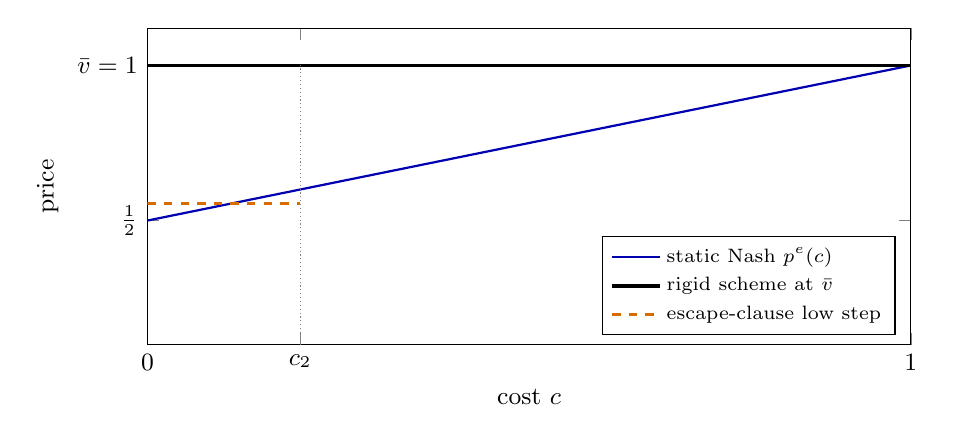
\begin{tikzpicture}
\begin{axis}[width=0.93\linewidth, height=5.6cm, xmin=0, xmax=1, ymin=0.1, ymax=1.12,
  xlabel={cost $c$}, ylabel={price}, xtick={0,0.2,1}, xticklabels={$0$,$c_2$,$1$},
  ytick={0.5,1}, yticklabels={$\frac{1}{2}$,$\bar v = 1$},
  legend style={font=\scriptsize, at={(0.98,0.03)}, anchor=south east}, legend cell align=left,
  tick label style={font=\small}, label style={font=\small}]
\addplot[blue!70!black, thick, domain=0:1, samples=2] {(1+x)/2};
\addlegendentry{static Nash $p^e(c)$}
\addplot[black, very thick, domain=0:1, samples=2] {1};
\addlegendentry{rigid scheme at $\bar v$}
\addplot[orange!85!black, very thick, dashed] coordinates {(0,0.5556) (0.2,0.5556)};
\addlegendentry{escape-clause low step}
\addplot[gray, densely dotted, forget plot] coordinates {(0.2,0.1) (0.2,1)};
\end{axis}
\end{tikzpicture}
\caption{Inelastic demand}
\end{subfigure}\hfill
\begin{subfigure}[b]{0.48\textwidth}
\centering
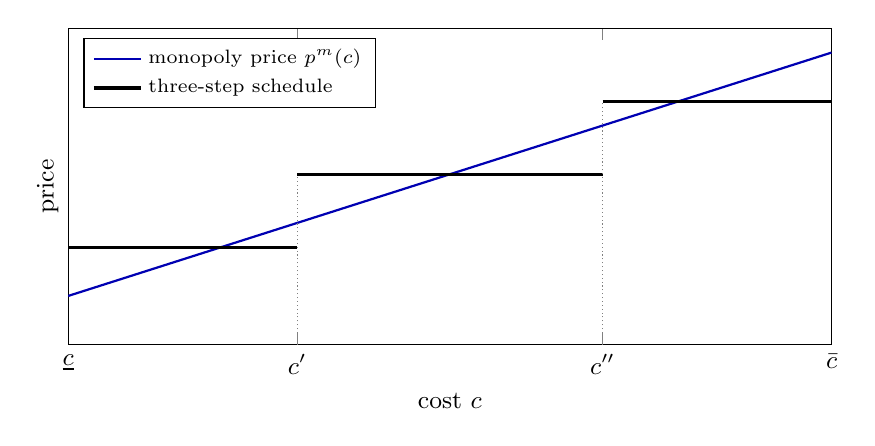
\begin{tikzpicture}
\begin{axis}[width=0.93\linewidth, height=5.6cm, xmin=0, xmax=1, ymin=0.4, ymax=1.05,
  xlabel={cost $c$}, ylabel={price}, xtick={0,0.3,0.7,1}, xticklabels={$\underline c$,$c'$,$c''$,$\bar c$},
  ytick=\empty,
  legend style={font=\scriptsize, at={(0.02,0.97)}, anchor=north west}, legend cell align=left,
  tick label style={font=\small}, label style={font=\small}]
\addplot[blue!70!black, thick, domain=0:1, samples=2] {(1+x)/2};
\addlegendentry{monopoly price $p^m(c)$}
\addplot[black, very thick] coordinates {(0,0.6) (0.3,0.6)};
\addlegendentry{three-step schedule}
\addplot[black, very thick, forget plot] coordinates {(0.3,0.75) (0.7,0.75)};
\addplot[black, very thick, forget plot] coordinates {(0.7,0.9) (1,0.9)};
\addplot[gray, densely dotted, forget plot] coordinates {(0.3,0.4) (0.3,0.75)};
\addplot[gray, densely dotted, forget plot] coordinates {(0.7,0.4) (0.7,0.9)};
\end{axis}
\end{tikzpicture}
\caption{Downward-sloping demand (schematic)}
\end{subfigure}
\caption{Collusive pricing schedules with private costs. Panel (a): two firms, costs uniform on $[0,1]$, reservation
value $\bar v = 1$. The static Nash schedule is $p^e(c) = \frac{1 + c}{2}$. The rigid scheme charges $\bar v$, which
is also the monopoly price, for every cost. A two-step escape-clause scheme charges $\bar v$ above the break point
$c_2$ and a low price on $[0, c_2)$ that keeps type $c_2$ indifferent (here $c_2 = 0.2$ and the low price is $0.556$).
In this uniform example the escape clause is not an equilibrium for $\delta < \delta^*$ (\cref{prop:12-abs-escape}),
so the panel only shows its shape. Panel (b): a three-step schedule. The bottom step lies below the monopoly price of
its highest type $c'$, and the top step lies above the monopoly price of its lowest type $c''$, as
\cref{prop:12-abs-downward}(ii) requires.}\label{fig:12-abs-schedules}
\end{figure}

\subsection{Impatient firms}\label{sec:12-abs-impatient}

Return to inelastic demand and suppose firms are not patient enough to make the off-schedule constraints slack.
After an off-schedule deviation, firms move to a war continuation value $w \in \mathcal V$, for example the worst SPPE
value or reversion to static Nash forever. Its per-period equivalent $\pi^w = (1 - \delta)w$ satisfies (ABS (7), p.~33)
\begin{equation}\label{eq:12-abs-piw}
0 \le \pi^w < \frac{1}{N}\pi(\bar v, \E c) .
\end{equation}
The first inequality holds in any SPPE. The second says that the war is a punishment relative to rigid collusion.
Here $\pi(\bar v, \E c) = \bar v - \E c$ is the expected profit from serving the whole market at $\bar v$.

\begin{proposition}[The threshold discount factor]\label{prop:12-abs-critical}
Let demand be inelastic. A stationary rigid scheme with price $p^r \in [\underline c, \bar v]$ and war value
$\pi^w$ satisfies the off-schedule constraints if and only if both
\begin{equation}\label{eq:12-abs-offschedule}
\frac{N - 1}{N}\,\pi(p^r, \underline c) \;\le\; \frac{\delta}{1 - \delta}\Bigl[\frac{1}{N}\pi(p^r, \E c) - \pi^w\Bigr]
\end{equation}
and
\begin{equation}\label{eq:12-abs-offschedule-high}
\frac{1}{N}\,(\bar c - p^r) \;\le\; \frac{\delta}{1 - \delta}\Bigl[\frac{1}{N}\pi(p^r, \E c) - \pi^w\Bigr]
\end{equation}
hold. If $p^r \ge \bar c$, \eqref{eq:12-abs-offschedule} implies \eqref{eq:12-abs-offschedule-high}. At
$p^r = \bar v$ the scheme therefore satisfies the off-schedule constraints if and only if $\delta \ge \delta^*$, where
\begin{equation}\label{eq:12-abs-deltastar}
\delta^* = \frac{(N - 1)\pi(\bar v, \underline c)}{(N - 1)\pi(\bar v, \underline c) + \pi(\bar v, \E c) - N\pi^w}
\;\in\;\Bigl(\frac{N - 1}{N},\, 1\Bigr).
\end{equation}
If $\delta < \delta^*$, no stationary rigid scheme at any price $p^r \le \bar v$ satisfies \eqref{eq:12-abs-offschedule},
so none satisfies the off-schedule constraints.
\end{proposition}

\begin{proof}
\emph{The constraints.} Under a rigid scheme a firm of type $c$ that undercuts $p^r$ slightly wins the whole market
instead of the share $\frac{1}{N}$. Its current gain is $\frac{N - 1}{N}\pi(p^r, c)$, which is largest for the
lowest type, since $\pi(p^r, c) = p^r - c$. A larger cut only lowers the price it receives. The deviation is
off-schedule, so the continuation drops from the collusive value, worth $\frac{1}{N}\pi(p^r, \E c)$ per period, to
the war, worth $\pi^w$ per period. The loss from the next period on is
$L \equiv \frac{\delta}{1 - \delta}[\frac{1}{N}\pi(p^r, \E c) - \pi^w]$. A type $c$ that raises its price above $p^r$
sells nothing. It earns zero today instead of $\frac{1}{N}(p^r - c)$, which is negative when $c > p^r$. Its current
gain is $\frac{1}{N}(c - p^r)$, which is largest for type $\bar c$, and it faces the same loss $L$. The binding
constraints are thus those of type $\underline c$ against a cut and of type $\bar c$ against a rise, which are
\eqref{eq:12-abs-offschedule} and \eqref{eq:12-abs-offschedule-high}. If $p^r \ge \bar c$, the left side of
\eqref{eq:12-abs-offschedule-high} is at most zero, while \eqref{eq:12-abs-offschedule} gives $L \ge 0$. Then
\eqref{eq:12-abs-offschedule} implies \eqref{eq:12-abs-offschedule-high}. \Cref{asm:12-abs} gives
$\bar v \ge \bar c$, so only \eqref{eq:12-abs-offschedule} matters at $p^r = \bar v$.

\emph{The threshold.} Let $a = (N - 1)\pi(\bar v, \underline c)$ and $b = \pi(\bar v, \E c) - N\pi^w$, which is
positive by \eqref{eq:12-abs-piw}. Multiply \eqref{eq:12-abs-offschedule} at $p^r = \bar v$ by $N(1 - \delta)$:
\begin{equation*}
(1 - \delta)a \le \delta b
\quad\Longleftrightarrow\quad
a \le \delta(a + b)
\quad\Longleftrightarrow\quad
\delta \ge \frac{a}{a + b} = \delta^* .
\end{equation*}
Since $b > 0$, $\delta^* < 1$. Moreover $\delta^* > \frac{N - 1}{N}$ if and only if $(N - 1)(a + b) < Na$, that is,
$(N - 1)b < a$, or $\pi(\bar v, \E c) - N\pi^w < \pi(\bar v, \underline c)$. This holds because
$\pi(\bar v, \underline c) > \pi(\bar v, \E c)$ and $\pi^w \ge 0$.

\emph{Lower rigid prices.} Both sides of \eqref{eq:12-abs-offschedule} are affine in $p^r$, with slopes
$\frac{N - 1}{N}$ on the left and $\frac{\delta}{(1 - \delta)N}$ on the right. If $\frac{N - 1}{N} < \delta < \delta^*$,
the right side rises faster, so the gap between the right and left sides increases in $p^r$. It is negative at
$p^r = \bar v$ and hence negative at every lower $p^r$. If $\delta \le \frac{N - 1}{N}$, the gap is non-increasing in
$p^r$, so the best case is $p^r = \underline c$. There the left side is zero and the right side is negative, since
$\pi(\underline c, \E c) = \underline c - \E c < 0$. In both cases \eqref{eq:12-abs-offschedule} fails (p.~52).
\end{proof}

ABS state \eqref{eq:12-abs-offschedule} as a necessary condition (p.~34). Constraints against price increases that
avoid a loss appear only in footnotes to later proofs (p.~53, footnote~45, and p.~54, footnote~46). In the second
the top price is $\bar v$, and they hold. They matter only for rigid prices below $\bar c$, where \eqref{eq:12-abs-offschedule} alone need not be
sufficient.

ABS extend the last statement to nonstationary schemes. If $\delta < \delta^*$, no SPPE has a rigid price in every
period (ABS Proposition 15, pp.~34 and 52--53). The reason is that the highest rigid price on the path would be
easier to sustain if it were kept forever. Combining the result with \cref{prop:12-abs-rigid}, if $F$ is log-concave and
$\delta \ge \delta^*$, the optimal SPPE has a rigid price at $\bar v$ (ABS Corollary 16, p.~35).

\begin{example}[Cost shocks make collusion harder]\label{ex:12-abs-uniform}
Let $N = 2$, costs uniform on $[0,1]$, $\bar v = 1$, and Nash reversion after an off-schedule deviation (p.~35). By
\cref{ex:12-abs-static-uniform}, $\pi^w = \frac{1}{6}$. Also $\pi(1, 0) = 1$ and $\pi(1, \E c) = \frac{1}{2}$. By
\eqref{eq:12-abs-deltastar},
\begin{equation*}
\delta^* = \frac{1}{1 + \frac{1}{2} - \frac{2}{6}} = \frac{1}{\frac{7}{6}} = \frac{6}{7} \approx 0.857 .
\end{equation*}
Without cost shocks, collusion at a price above a common cost needs only $\delta \ge \frac{1}{2}$ (\cref{prop:12-bertrand}).
The same computation for $N$ firms uses $\pi^w = \frac{1}{N(N + 1)}$ and gives
\begin{equation*}
\delta^*(N) = \frac{N - 1}{(N - 1) + \frac{1}{2} - \frac{1}{N + 1}} = \frac{2(N + 1)}{2N + 3},
\end{equation*}
so $\delta^*(3) = \frac{8}{9}$ and $\delta^*(4) = \frac{10}{11}$, against $\frac{2}{3}$ and $\frac{3}{4}$ without
cost shocks. (This general formula is our own computation. It simplifies because the denominator equals
$\frac{(2N + 3)(N - 1)}{2(N + 1)}$.)
\end{example}

The benchmark $\frac{N - 1}{N}$ is the value of \eqref{eq:12-abs-deltastar} when $\underline c = \E c$ and
$\pi^w = 0$. Cost fluctuations raise the required patience because the scheme must survive the period in which a firm
draws a cost far below the one it expects in the future (p.~35). This holds even if the punishment drives profits to
zero, and the threshold rises further when the punishment is milder. The result fits the common view that collusion is
harder when costs vary across firms and over time \citep[p.~205]{Scherer1980}.

\begin{proposition}[No wars for impatient firms]\label{prop:12-abs-impatient-nowars}
Let demand be inelastic, and let $F$ and $\delta$ be arbitrary. Consider an SPPE with schedule $p$ and continuation
function $v$, and let $z \equiv \sup_{c'}\E_{-i}v(p(c'), \mathbf p_{-i})$. Suppose that
$\E_{-i}v(p(c), \mathbf p_{-i}) < z$ for some $c$, and that a mild regularity condition holds at the top step. Then
there is an SPPE with the same expected payoff in which the continuation value equals $z$ after every on-schedule
price (ABS Proposition 17, p.~37).
\end{proposition}

The proof compares off-schedule constraints. Let $c_k$ be the lowest type on a flat step. With war continuation $w$,
this type's constraint in the original scheme is (ABS (11), p.~53)
\begin{equation*}
\pi\bigl(p(c_k), c_k\bigr)\bigl[(1 - F(c_k))^{N-1} - M(c_k; p)\bigr] \le \delta z - \mathcal T(c_k) - \delta w .
\end{equation*}
Here $\mathcal T(c_k) = \delta[z - \E_{-i}v(p(c_k), \mathbf p_{-i})]$, and the bracket on the left is the gain in
the probability of winning from a slight undercut. The no-war alternative of \cref{lem:12-abs-nowar-equiv} has the same
allocation and a price $\tilde p(c_k) < p(c_k)$ wherever $\mathcal T(c_k) > 0$. Its constraint is (ABS (12))
\begin{equation*}
\pi\bigl(\tilde p(c_k), c_k\bigr)\bigl[(1 - F(c_k))^{N-1} - M(c_k; p)\bigr] \le \delta z - \delta w .
\end{equation*}
The left side is smaller and the right side larger. Moving profit from the present (a lower price today) to the future
(no war tomorrow) reduces the temptation to cheat and raises the value of cooperation at the same time. Wars are thus
doubly harmful for impatient firms with inelastic demand. With downward-sloping demand a war on a step can still help
by relaxing the constraints of types on lower steps (pp.~37--38).

\casehead{An escape clause}
Impatient firms cannot keep a rigid price, but they may support a two-step scheme with a high price $\bar v$ and a
lower price for rare low-cost draws.

\begin{proposition}[Escape clause]\label{prop:12-abs-escape}
Let demand be inelastic and $N = 2$. If
\begin{equation}\label{eq:12-abs-escape}
f(\underline c) < \frac{\frac{1}{2}\pi(\bar v, \E c) - \pi^w}{\pi(\bar v, \underline c)\,\pi^w},
\end{equation}
there is $\delta^\circ < \delta^*$ such that, for every $\delta \in (\delta^\circ, \delta^*)$, a two-step schedule with
prices $p_2 = \bar v > p_1$ and a break point $c_2 \in (\underline c, \bar c)$ is an SPPE (ABS Proposition 18,
p.~39).
\end{proposition}

The working paper prints the denominator of \eqref{eq:12-abs-escape} as $\bar v\,\pi^w$. The two agree when
$\underline c = 0$, as in all its examples. For general $\underline c$ the slope comparison in its proof gives
$\pi(\bar v, \underline c)\,\pi^w$, as we show below. With $\underline c > 0$ the printed condition is a stronger
sufficient condition.

We do not reproduce the whole existence proof (pp.~53--55), which is a continuity argument. At $\delta = \delta^*$ and
$c_2 = \underline c$ the two-step scheme is the rigid one, and its off-schedule constraints bind. Under
\eqref{eq:12-abs-escape}, raising $c_2$ slightly makes these constraints slack. The slack lets a two-step scheme
survive for $\delta$ slightly below $\delta^*$. The binding constraint for small $c_2$ is that of type $c_2$
undercutting $\bar v$. Its current gain is $\Omega(c_2) = \frac{1}{2}\pi(\bar v, c_2)[1 - F(c_2)]$. Let $W(c_2)$
be the expected per-period profit of the two-step scheme minus $\pi^w$, so the loss from a war is
$\frac{\delta}{1-\delta}W(c_2)$. Differentiating the expressions for $\Omega$ and $W$ on p.~54 of ABS at
$c_2 = \underline c$ gives
\begin{equation*}
\Omega'(\underline c) = -\frac{1}{2}\bigl[1 + f(\underline c)\,\pi(\bar v, \underline c)\bigr],
\qquad
W'(\underline c) = -\frac{1}{2}f(\underline c)\,\pi(\bar v, \E c) .
\end{equation*}
The constraint gains slack as $c_2$ rises from $\underline c$ if $\frac{\delta^*}{1-\delta^*}W'(\underline c) >
\Omega'(\underline c)$. With $N = 2$, \eqref{eq:12-abs-deltastar} gives
$\frac{\delta^*}{1-\delta^*} = \frac{\pi(\bar v, \underline c)}{\pi(\bar v, \E c) - 2\pi^w}$, and the inequality
rearranges to \eqref{eq:12-abs-escape}.

The on-schedule constraint pins down the low price (ABS (13), p.~53). Type $c_2$ must be indifferent between the two
steps. With two firms, a firm on the low step wins unless the rival is also on it, in which case they tie, so
$M_1 = 1 - \frac{F(c_2)}{2}$. A firm on the high step wins half the time when the rival is also high, so
$M_2 = \frac{1 - F(c_2)}{2}$. Indifference, $(p_1 - c_2)M_1 = (\bar v - c_2)M_2$, gives
\begin{equation}\label{eq:12-abs-p1}
p_1 = c_2 + (\bar v - c_2)\,\frac{1 - F(c_2)}{2 - F(c_2)} .
\end{equation}
As $c_2 \to \underline c$, $p_1 \to \frac{\bar v + \underline c}{2}$. With $\underline c$ near zero the low price is
about half the high price, the 50 percent cut that ABS report for their construction with $c_2$ close to $\underline c$
(p.~39, footnote 32). In the uniform example with $c_2 = 0.2$, $p_1 = 0.2 + \frac{0.64}{1.8} = 0.556$
(\cref{fig:12-abs-schedules}).

The escape clause works through two effects (pp.~38--39). The lowest-cost firm now expects more than the share
$\frac{1}{N}$, at a lower price, so its gain from undercutting is smaller. With $c_2$ close to $\underline c$, one can
check from \eqref{eq:12-abs-p1} that the most tempted type becomes the break-point type $c_2$. Its best deviation is
a price just below $\bar v$, and its cost exceeds $\underline c$. Against this, a two-step scheme
earns less than the rigid scheme when $F$ is log-concave, so a deviator also has less to lose. A small density at the
bottom keeps the second effect small, which is what \eqref{eq:12-abs-escape} requires. The condition is restrictive.
For $F(c) = c^\alpha$ on $[0,1]$ it holds when $\alpha > 1$ and fails for $\alpha \le 1$ (p.~39). In the uniform
example the right side of \eqref{eq:12-abs-escape} is $\frac{\frac{1}{4} - \frac{1}{6}}{\frac{1}{6}} = \frac{1}{2} <
1 = f(0)$. There, two-step schemes fail the off-schedule constraint for exactly the same discount factors as the rigid
scheme (pp.~39--40).

The escape clause has an interpretation that matters for reading cartel histories (pp.~39, 47). Collusion among
impatient firms may be marked by occasional, large price cuts by single firms after favorable cost draws, which rivals
do not punish. They are a permitted exception, firm by firm, much as \citet{RotembergSaloner1986} allow prices to
fall when demand is high. In that model, however, all firms adjust together in response to a public shock.

Finally, under log-concavity and a non-decreasing density, an optimal stationary SPPE for impatient firms that beats
Nash has no open interval of strictly increasing prices (ABS Proposition 19, p.~41). It is a step function: partial
rigidity. The analysis is a static mechanism design problem with two unusual features. The participation constraints
depend on the type, and they are endogenous, because the value of the outside option depends on the scheme itself
(pp.~40--42).

\subsection{Asymmetric schemes}\label{sec:12-abs-asymmetric}

Symmetric equilibria allow only wasteful transfers, borne by all firms. Asymmetric perfect public equilibria also let
firms transfer value from one firm to another through the continuation, for example by favoring in future periods a
firm that has sold little (p.~43). ABS illustrate with two simple schemes, using two firms, inelastic demand, uniform
costs on $[0,1]$, $\bar v = 1$ and Nash reversion.

\casehead{Taking turns}
In a \emph{take-turns} scheme the firms alternate in serving the market at $\bar v$. With inelastic demand it offers
no efficiency gain over rigid pricing, since the winner's identity is independent of costs. It needs more patience.
The most tempted firm is one whose turn it is to sit out and which has drawn cost zero. Undercutting gives it
$\pi(1, 0) = 1$ now and the Nash value $\frac{\delta}{1 - \delta}\cdot\frac{1}{6}$ afterward. Conforming gives nothing
now and the expected profit $\frac{1}{2}$ in every other period from the next one on, worth
$\frac{\delta}{1 - \delta^2}\cdot\frac{1}{2}$. The constraint is
\begin{equation*}
\frac{\delta}{2(1 - \delta^2)} \ge 1 + \frac{\delta}{6(1 - \delta)} .
\end{equation*}
Multiply by $6(1 - \delta^2)$ to get $3\delta \ge 6(1 - \delta^2) + \delta(1 + \delta)$, that is,
$5\delta^2 + 2\delta - 6 \ge 0$. The positive root is $\frac{\sqrt{31} - 1}{5} = 0.9135$, above $\delta^* = 0.857$
(p.~44, footnote 38).

\casehead{A two-price scheme}
In the \emph{two-price scheme} $(p^l, \bar v)$, each firm may charge the low price $p^l$ exactly once in every
two-period cycle and $\bar v$ in the other period (p.~44). In the first period of a cycle a firm chooses between the
sequences $(p^l, \bar v)$ and $(\bar v, p^l)$. Using the low price now forfeits it tomorrow, when the firm's cost may
be lower, so only firms with low current costs take it. Types below a cutoff $c^\dagger$ choose $(p^l, \bar v)$. (ABS
write $\theta^*$ for the cutoff.)
Indifference of type $c^\dagger$ when the rival uses the same cutoff gives (ABS (10), p.~45)
\begin{multline*}
F(c^\dagger)\,\frac{\pi(p^l, c^\dagger) + \delta\pi(\bar v, \E c)}{2} + [1 - F(c^\dagger)]\,\pi(p^l, c^\dagger) \\
= F(c^\dagger)\,\delta\pi(p^l, \E c) + [1 - F(c^\dagger)]\,\frac{\pi(\bar v, c^\dagger) + \delta\pi(p^l, \E c)}{2} .
\end{multline*}
The left side is the expected two-period profit from using the low price first, and the right side from using it
second.\footnote{The equation printed as (10) in the working paper (p.~45) has no factor $\delta$ on the term
$\pi(\bar v, \E c)$ in its top line. We restore it, because the second-period profit must be discounted like every
other second-period term. With the factor restored, the approximation $c^\dagger \approx \frac{2 - \delta}{2}$ that ABS
state follows, and without it the approximation does not hold.} With $p^l$ close to $\bar v = 1$ and uniform costs, let $x = c^\dagger = F(c^\dagger)$. The difference between
the two sides reduces to $\frac{1 - x}{2} - \frac{\delta}{4}$, so $c^\dagger \approx \frac{2 - \delta}{2}$, which lies in
$(\frac{1}{2}, 1]$ (p.~45). A firm with cost below $c^\dagger$ uses its low price in the first period, so some sorting
occurs at almost no price distortion, and the scheme beats rigid pricing. Sorting rises with $\delta$, and as
$\delta \to 1$ the cutoff tends to the median cost. The scheme still needs patience, $\delta \ge \delta^{**} \approx
0.88$, above $\delta^*$ though below the take-turns threshold (p.~46, footnote 41). Its novel prediction is that a
firm's market share is negatively correlated over time. ABS suggest that such schemes suit small groups of firms that
track each other's sales and communicate explicitly. \citet{AtheyBagwell2001} study optimal asymmetric collusion with
communication about costs.

\subsection{Testable implications, limitations and contribution}\label{sec:12-abs-assessment}

\Cref{tab:12-abs-results} collects the main results. They yield several predictions (pp.~46--48). Collusive prices
are rigid with respect to firm-specific, privately observed cost shocks. They respond to public cost shocks, such as
a change in a common wholesale price, because the whole scheme can be re-tailored to a public change. Prices are more
rigid in concentrated, collusive industries. Optimal collusion among patient firms involves no price wars, unlike
\cref{sec:12-gp-original}. Impatient cartels may show occasional large price cuts by single firms that rivals ignore.
ABS offer this as an alternative reading of apparent unpunished cheating, an issue raised for the Sugar Institute by
\citet{GenesoveMullin2001}, whose working-paper version ABS cite (p.~47, footnote 43). ABS also combine private costs
with the persistent demand phases of \citet{BagwellStaiger1997}. They conjecture that off-schedule constraints are
easier to meet in booms when growth rates are positively correlated, so prices may be more rigid in booms (p.~48).

\begin{table}[htbp]
\centering
\caption{Optimal symmetric collusion with private costs}\label{tab:12-abs-results}
\begin{tabularx}{\textwidth}{@{}l>{\raggedright\arraybackslash}X>{\raggedright\arraybackslash}X@{}}
\toprule
 & Inelastic demand & Downward-sloping demand \\
\midrule
Fully sorting schemes & Best is repeated static Nash (\cref{prop:12-abs-fullsort}) & Best is repeated static Nash, and all others are strictly worse (\cref{prop:12-abs-downward}(i)) \\
Patient firms: wars & Never needed (\cref{prop:12-abs-nowars}) & Never at the top or bottom step, possible only on intermediate steps (\cref{prop:12-abs-downward}(ii) and (iii)) \\
Patient firms: prices & Rigid at $\bar v$ if $F$ is log-concave (\cref{prop:12-abs-rigid}) & Rigid at the bottom, single rigid price if demand is inelastic enough and $F$ log-concave (\cref{prop:12-abs-downward}(iv)) \\
Impatient firms & Rigid price at $\bar v$ if and only if $\delta \ge \delta^*$ (\cref{prop:12-abs-critical}), no wars (\cref{prop:12-abs-impatient-nowars}), escape clause for small $f(\underline c)$ (\cref{prop:12-abs-escape}), step functions & Wars on a step may relax lower types' constraints \\
\bottomrule
\end{tabularx}

\smallskip
\begin{minipage}{0.95\textwidth}
\footnotesize Notes: SPPE, costs \iid\ across firms and periods. Source: \citet{AtheyBagwellSanchirico2004},
working-paper version, Propositions 8 to 19.
\end{minipage}
\end{table}

\casehead{Limitations}
The analysis restricts attention to symmetric equilibria, which ABS defend on three grounds (pp.~6--7). Under many
conditions the optimal SPPE is stationary and simple. Symmetric schemes capture the fear of industry-wide breakdowns,
and they are the only option when the identity of the seller is not observed. Asymmetric schemes do better when firms
are patient and sophisticated. Costs are \iid\ over time. With persistent costs a firm's current price reveals
information about its future costs, which changes the incentive problem. \citet{AtheyBagwell2008} study that case.
The clean results rely on inelastic demand, and with downward-sloping demand the characterization is partial. There
is no communication in the symmetric analysis. \citet[p.~2431]{HarringtonSkrzypacz2011} contrast their setting with
the asymmetric extension of this analysis with communication \citep{AtheyBagwell2001,AtheyBagwell2008}. There, prices
are public and firms report private costs so that the low-cost firm can be given more market share. In the model of
Harrington and Skrzypacz, prices and sales are private, and firms report sales so that the cartel can monitor
compliance (\cref{sec:12-hs}).

\casehead{Contribution}
ABS identify a basic trade-off for colluding firms with private information. Sorting by cost buys productive
efficiency at an informational cost, paid in distorted prices or in wars. Rigidity removes the informational cost at
the price of efficiency. They show that rigidity usually wins and that optimal collusion rarely needs wars, which gives
an equilibrium foundation to the old association between collusion and rigid prices. Methodologically, they connect
repeated games with hidden information to static mechanism design, with restricted transfers and endogenous,
type-dependent participation constraints. \Cref{sec:12-cartels} turns to the way real cartels use communication to
relax these constraints.

\section{How Cartels Organize: Communication, Facilitating Practices, and Transfers}\label{sec:12-cartels}

The models of \cref{sec:12-perfect,sec:12-demand,sec:12-public,sec:12-private-costs} treat collusion as an
equilibrium of a non-cooperative repeated game. Firms in those models never meet, never talk and never sign
anything. The cartels that antitrust authorities prosecute look different. Their members meet regularly, agree on
target prices, divide sales, exchange sales figures, hire auditors and pay one another compensation. This section
asks what these practices accomplish, and why firms take the legal risk of using them when tacit collusion is
available in theory.

The answer turns on information. Suppose that monitoring is perfect and that demand and costs are common
knowledge. An agreement can then do little more than select one of the many equilibria of the repeated game.
Once prices, sales or costs are private, communication and transfers change what the cartel can enforce.
\Cref{sec:12-anatomy} describes the common design of explicit cartels and maps each design element to the problem
it solves. \Cref{sec:12-facilitating} studies business practices and market features that relax the incentive
constraints of \cref{sec:12-perfect} without an explicit agreement, including multimarket contact and the threat of
entry. \Cref{sec:12-hs} develops in depth the model
of \citet{HarringtonSkrzypacz2011}. It shows that quotas, self-reported sales and transfers form an equilibrium
when prices and sales are private. \Cref{sec:12-bm-preview} previews a model in which cartels tolerate deliberate
cheating, which \cref{sec:13-imperfect} develops in full.

\subsection{The anatomy of explicit cartels}\label{sec:12-anatomy}

A cartel, as defined in \cref{sec:12-forms}, colludes explicitly: its members coordinate through direct
communication about prices, quantities, customers or bids. The repeated-game models of this chapter apply to
explicit and tacit collusion alike. They describe which outcomes the threat of future competition can enforce,
whatever the means by which firms coordinate. The records of prosecuted cartels raise a second question, which
concerns the organization of the agreement itself.

\citet[pp.~105--108]{MarshallMarx2012} build their account of cartel organization on \citet{Stigler1964}. For them
the central problem of a cartel is to avert secret deviations by its members. A cartel solves it with three
complementary \emph{collusive structures}. \emph{Pricing structures} implement price increases and output
reductions. \emph{Allocation structures} divide the collusive gain, through market shares, territories or customers,
and set up mechanisms to redistribute gains among members. \emph{Enforcement structures} monitor compliance and
establish the threat of punishment. Marshall and Marx stress that each structure is insufficient alone. An agreement
on price without an agreement on allocation and enforcement will almost surely collapse through secret deviations.
A cartel that has suppressed rivalry among its members can then turn to the forces outside it, such as entrants,
producers of substitutes, buyers and suppliers \citep[pp.~143--144]{MarshallMarx2012}. We first state the two
constraints that every cartel must satisfy. We then take four internal elements in turn, treating monitoring
separately from punishment, and attach each to the theory of this chapter. \Cref{tab:12-cartel-elements} summarizes
the mapping, and the subsection ends with the plus factors that these elements leave behind.

\casehead{Two constraints}
\citet[pp.~187--188]{AskerNocke2021} organize the economics of cartels around two constraints. Let $\mathcal C$ be a
set of potential members. Firm $i \in \mathcal C$ joins only if it satisfies the \emph{participation constraint}, also
called the internal stability condition,
\begin{equation}\label{eq:12-participation}
V_i^{\mathrm{comp}} \;\le\; V_i^{\mathrm{coll}} - \eta_i .
\end{equation}
Here $V_i^{\mathrm{coll}}$ is the firm's value inside the cartel. $V_i^{\mathrm{comp}}$ is its value if it stays out
while the other firms in $\mathcal C$ join. The one-time cost $\eta_i$ of joining captures the frictions of organizing.
No court enforces a cartel agreement, so each member must also satisfy the \emph{no-cheating constraint}
\begin{equation}\label{eq:12-no-cheating}
V_i^{\mathrm{coll}} \;\ge\; \pi_i^{\mathrm{dev}} + \delta\,V_i^{\mathrm{ret}} .
\end{equation}
Here $\pi_i^{\mathrm{dev}}$ is the profit in the period of cheating and $V_i^{\mathrm{ret}}$ the continuation value
after retaliation. Constraint \eqref{eq:12-no-cheating} is the incentive constraint of every model so far.
Constraint \eqref{eq:12-participation} is new. It asks whether each firm wants to be inside at all.

The participation constraint can fail even when collusion is very profitable. \citet[pp.~192--193]{AskerNocke2021}
give an example. Six firms with marginal cost $c$ compete in quantities against inverse demand $P(Q) = a - bQ$. Let
$A = \frac{(a - c)^2}{b}$. In the Cournot equilibrium with $M$ symmetric players each earns $\frac{A}{(M + 1)^2}$, so
each of the six firms earns $\frac{A}{49}$. A cartel of all six earns the monopoly profit $\frac{A}{4}$, or $\frac{A}{24}$
per member. Suppose one firm refuses to join. The other five then act as one player in a Cournot duopoly with the
outsider, and each of the two players earns $\frac{A}{9}$. Each insider gets $\frac{A}{45} > \frac{A}{49}$, so the
five still gain by colluding. The outsider gets $\frac{A}{9}$, far more than $\frac{A}{24}$. Every firm would like to be
the one that stays out. Negotiations over who is in and who gets what are therefore hard, and a threat to stay out
unless paid extra is credible. The example mirrors the merger paradox of quantity competition. \citet{BosHarrington2010}
endogenize cartel formation among firms with different capacities. Smaller firms are more likely to stay out. The
cartel sets a price that serves as an umbrella, and the noncartel firms price below it and produce at capacity.

\casehead{Agreeing on price}
Repeated-game theory predicts a whole set of sustainable prices. In the Bertrand supergame every price between
marginal cost and the monopoly price is sustainable once $\delta \ge 1 - \frac{1}{N}$
(\cref{cor:12-bertrand-any-price}). Firms that collude tacitly must somehow land on the same element of this set.
An explicit agreement solves this selection problem directly. The members of the lysine cartel, for example, met
in July 1992. They agreed to raise the price to \$1.05 per pound by September 30, 1992, and to \$1.20 per pound by
December 30, 1992 \citep[p.~2426]{HarringtonSkrzypacz2011}. A notorious invitation to collude shows how a single
proposal can do the same. In 1982 Robert Crandall, chief executive of American Airlines, telephoned Howard Putnam of
Braniff, a rival on routes out of Dallas-Fort Worth. Crandall proposed that Braniff raise its fares by twenty percent
and promised to raise his own the next morning. Putnam recorded the call and turned it over to the Department of
Justice \citep[pp.~188--189]{AskerNocke2021}. The proposal named the price point, a simple rule of thumb across many
fares, and left the threat of continued fare wars implicit. \citet{GreenPorter1984} made a similar point about their
own trigger strategies. In view of their complexity and the close coordination they need, it seemed natural to
assume that the equilibrium arises from an explicit agreement (p.~89, footnote~5).

Tacit coordination is possible, but it can be slow. \citet{ByrneDeRoos2019} study retail gasoline in Perth, Australia,
from 2001 to 2015 \citep[pp.~189--191]{AskerNocke2021}. Stations had to commit to prices a day ahead and post them
on Fuelwatch, a government website meant to help consumers search. Between 2009 and 2013, as Asker and Nocke date the
episode, the BP chain led the market to higher margins and synchronized price jumps. Byrne and de Roos describe a
three-year transition from April 2009 to August 2012 \citep[p.~592]{ByrneDeRoos2019}. BP first raised prices on Wednesdays, and by mid-2010 Caltex, the
next-largest chain, followed with jumps on Thursdays. BP then moved its own jumps to Thursday and occasionally
stopped leading, to test whether the market would coordinate without it. The market settled on weekly price jumps
on Thursdays, followed by daily price cuts of 2 cents per liter between jumps
\citep[pp.~596--597 and 607--608]{ByrneDeRoos2019}. Byrne and de Roos read the episode as coordination learned
through prices, but they state that they cannot rule out explicit communication between firms, such as phone calls
\citep[p.~617]{ByrneDeRoos2019}. \citet[p.~191]{AskerNocke2021} conclude only that market interaction itself may
provide enough communication for coordination.

Laboratory evidence points the same way. \citet{CooperKuhn2014} study a two-stage game that is a reduced form of a
repeated Bertrand game. The first stage is a pricing game with a low, a medium and a high price. The second is a
coordination game with three equilibria, which are Pareto ranked. Without communication, matched subjects reach the
high price in the first stage in fewer than 10 percent of cases. With limited communication the share is at most 50
percent, and it falls below 20 percent as subjects gain experience. In the least restrictive treatment, which allows
unrestricted chat, the share exceeds 80 percent \citep[p.~191]{AskerNocke2021}. Kaplow cites a coordination
experiment with a less regular pattern (\cref{sec:12-kaplow}).

Pricing algorithms raise the question in a new form \citep[p.~192]{AskerNocke2021}. In simulations by
\citet{CalvanoEtAl2020}, agents that learn to play a repeated Bertrand game through a reinforcement-learning
algorithm reach supracompetitive prices. \citet{AssadEtAl2020} find that the inferred adoption of algorithmic
pricing by German gasoline retailers coincided with increases in margins of up to 28 percent. Whether such outcomes
count as agreements is the question of \cref{sec:12-kaplow}.

Agreement is harder when members differ. A low-cost
firm prefers a lower collusive price than a high-cost firm, and asymmetries change who gains most from a deviation
(\cref{sec:12-perfect}). The resulting bargaining problems are frequent in the historical record.
In the case studies surveyed by \citet{LevensteinSuslow2006}, bargaining problems end more cartels than secret
cheating does (\cref{sec:12-success}).

\casehead{Allocating sales}
Most documented cartels agree on an allocation as well as a price. Lysine and citric acid used quotas in
quantities or in market shares (\cref{tab:12-hs-allocations}). The nucleotide cartel of
\cref{sec:13-imperfect-evidence} assigned customers. Other cartels drew exclusive territories, and bidding rings
used bid rotation or knockout auctions (\cref{sec:13-asker}). An allocation does three things. First, it turns the
problem of policing secret price cuts into a problem of policing quantities. A firm that steals customers ends up
with sales above its quota, and sales are easier to count than the discounts behind them. This is the logic of
\citet{Stigler1964}, who saw the detection of secret price cuts through shifts of customers as the central
problem of oligopoly (\cref{sec:12-public}). Second, an allocation fixes the division of the collusive profit,
which removes one source of bargaining. Third, an allocation can raise joint profit by directing production to the
lowest-cost members. \Cref{sec:12-private-costs} shows the limits of this third role. Without communication, firms
with private costs often do best with a rigid price that ignores costs (\cref{prop:12-abs-rigid}). When firms can
report their costs, the cartel can give more of the market to the member with the lowest cost
\citep{AtheyBagwell2001}.

\casehead{Monitoring}
A cartel monitors compliance by gathering information about the prices or sales of its members. In lysine one
member compiled self-reported sales into monthly ``scorecards''. In citric acid outside Swiss auditors checked the
reports. The Sugar Institute of \cref{sec:13-sugar-institute} collected reports through a trade association, and
many cartels relied on published price lists. \citet[p.~106]{MarshallMarx2012} distinguish two kinds of deviation
that monitoring must handle. \emph{Unintentional deviations} arise, for example, when a sales staff that does not
know of the cartel bids too aggressively or wins a customer it should not have won. If management acknowledges such
mistakes quickly, the cartel can correct them by reallocating future contracts, by subcontracting, or by
end-of-period transfers. \emph{Secret deviations} are special deals that the perpetrator does not acknowledge, and
uncovering them requires costly intelligence. Many cartels delegate part of the monitoring to outsiders. Marshall
and Marx review the twenty-two decisions on industrial-product cartels that the European Commission issued from 2000
through 2005 (pp.~125--127). In eleven of them, the decision mentions a third-party facilitator, such as a trade
association or a consulting or accounting firm (their Table~6.1, our count). The Swiss consultancy AC-Treuhand, which
served several European chemical cartels, was itself prosecuted for its services to the heat-stabilizers cartel
\citep[p.~197]{AskerNocke2021}. The information structure decides which theory applies.
In \citet{GreenPorter1984}, firms see a public price that depends on hidden outputs and on demand
(\cref{sec:12-public}). In \citet{AtheyBagwellSanchirico2004}, prices are public and costs are private
(\cref{sec:12-private-costs}). In the industrial cartels studied by \citet{HarringtonSkrzypacz2011}, both prices
and sales were private, so monitoring had to rely on what firms told one another (\cref{sec:12-hs}).

\casehead{Enforcement and transfers}
The basic enforcement device of repeated-game theory is a price war that hurts every member. A war destroys
profit, and it punishes the innocent along with the guilty. Many cartels also used targeted compensation. Under
the lysine cartel's ``guaranteed buy-ins'' and the citric acid cartel's ``buy-back system'', a firm that sold more
than its quota bought output from members below quota. The International Steel Agreement of 1926 ran a common fund
into which over-quota producers paid (\cref{sec:12-hs} gives the details). An interfirm sale at a price above cost transfers surplus from
the buyer to the seller. Such sales also aroused little suspicion, because they were common in these industries
\citep[p.~2433]{HarringtonSkrzypacz2011}. Transfers of this kind are \emph{asymmetric punishments}. They penalize
the member that sold too much and leave industry profit intact. \citet{HarringtonSkrzypacz2007} first argued that
asymmetric punishments are essential to effective collusion when firms observe one another's sales
\citep[p.~2442]{HarringtonSkrzypacz2011}. \Cref{sec:12-hs} extends the argument to sales that are private.

\begin{table}[htbp]
\centering
\caption{The design elements of explicit cartels}
\label{tab:12-cartel-elements}
\small
\begin{threeparttable}
\begin{tabularx}{\textwidth}{@{}>{\raggedright\arraybackslash}p{2.0cm}
  >{\raggedright\arraybackslash}X >{\raggedright\arraybackslash}X >{\raggedright\arraybackslash}p{2.9cm}@{}}
\toprule
Element & Problem it solves & Documented examples & Theory in this book \\
\midrule
Price & Select one price from the set of sustainable prices. Settle the level among members with different
interests. & Lysine targets of \$1.05 and \$1.20 per pound (1992) & \cref{cor:12-bertrand-any-price},
\cref{sec:12-success} \\
\addlinespace
Allocation & Turn secret price cuts into visible excess sales. Divide the gains. Direct output to efficient
members. & Lysine and citric acid quotas (\cref{tab:12-hs-allocations}). Customer allocation (nucleotides). Bid
rotation and knockouts (stamp ring). & \cref{sec:12-public,sec:12-private-costs,sec:12-hs} \\
\addlinespace
Monitoring & Verify compliance when prices or sales are private. & Monthly sales scorecards (lysine). Swiss
auditors (citric acid). Trade association rules and reports (Sugar Institute). &
\cref{sec:12-public,sec:12-hs,sec:13-information} \\
\addlinespace
Enforcement & Deter deviations at the least cost to the cartel. & Guaranteed buy-ins (lysine). Buy-backs (citric
acid). A fund of \$4 and \$2 per ton (steel, 1926). Price wars (railroads, 1880s). &
\cref{sec:12-perfect,sec:12-hs,sec:13-jec} \\
\bottomrule
\end{tabularx}
\begin{tablenotes}\footnotesize
\item Notes: Our synthesis. The examples come from \citet{HarringtonSkrzypacz2011}, \citet{GenesoveMullin2001},
\citet{BernheimMadsen2017} and \citet{Asker2010}, which \cref{ch:collusion-evidence} discusses.
\end{tablenotes}
\end{threeparttable}
\end{table}

\casehead{Plus factors and the cost of communication}
Communication helps a cartel, but it also creates evidence. Price-fixing law in the United States and the European
Union condemns agreements, and proof of an agreement usually rests on proof of communication
(\cref{sec:12-enforcement}). Economists who assist courts therefore look for \emph{plus factors}, the body of
economic circumstantial evidence of collusion beyond the parallel movement of prices. A plus factor that delivers
a strong inference of collusion is a \emph{super-plus factor} \citep[p.~213]{MarshallMarx2012}. Marshall and Marx
organize plus factors by the collusive structure that generates them, in nine baskets of cartel conduct
(pp.~213--214). Pricing structures produce four of them: (1) prices elevated above their level without the
conspiracy and (2) industry output restricted below that level. They also produce (3) steps to reduce buyers'
resistance to price increases and (4) changes in incentives within member firms that inhibit rivalry between them. Allocation structures produce
(5) an allocation of the collusive gain among members and (6) redistributions of gains and losses that maintain
compliance, such as end-of-period purchases from one another (p.~106). Enforcement structures produce
(7) communication and monitoring, especially of production, sales and market shares, and (8) a readiness to
abandon collusion if members keep cheating. A cartel that has suppressed rivalry among its members may finally seek
further profits through (9) dominant-firm conduct. Courts often ask in addition for actions that would be against a
firm's interest if taken independently \citep[p.~110]{Kaplow2013}.

Marshall and Marx measure the evidential value of a plus factor with Bayes' rule (pp.~234--235). Let $C$ be the event
that the firms collude and $F$ the event that a plus factor is observed. Their equation (11.1) is
\begin{equation}\label{eq:12-plus-bayes}
\Pr[C \mid F] = \frac{\Pr[F \mid C]\,\Pr[C]}{\Pr[F \mid C]\,\Pr[C] + \Pr[F \mid \text{not } C]\,\Pr[\text{not } C]} .
\end{equation}
An observed conduct is a plus factor if $\Pr[C \mid F] > \Pr[C]$. Define the \emph{strength} of the plus factor and
the baseline odds against a cartel as
\begin{equation*}
S = \frac{\Pr[F \mid C]}{\Pr[F \mid \text{not } C]} ,
\qquad
O = \frac{\Pr[\text{not } C]}{\Pr[C]} .
\end{equation*}
Divide the numerator and the denominator of \eqref{eq:12-plus-bayes} by $\Pr[F \mid C]\Pr[C]$. The second term of the
denominator becomes $\frac{O}{S}$, so
\begin{equation}\label{eq:12-plus-strength}
\Pr[C \mid F] = \frac{1}{1 + \frac{O}{S}}
\end{equation}
(p.~235, note~42). The posterior rises with $S$, and the conduct is a plus factor if and only if $S > 1$. A
super-plus factor is one that is unlikely without a cartel. When $\Pr[F \mid \text{not } C]$ is close to zero, $S$ is
large and $\Pr[C \mid F]$ is close to one. Marshall and Marx give an example (p.~236, note~44). Fit an econometric
model to noncollusive benchmark data and build a 95 percent \emph{prediction band} for the actual price path. A
prediction band covers realized prices, so it adds the noise in prices to the estimation error. Here it must cover
the whole path at once with probability 0.95 when there is no cartel. Let $F$ be the event that some actual price
leaves the band, so that $\Pr[F \mid \text{not } C] = 0.05$. Marshall and Marx speak of confidence bounds. A
confidence band for the mean price would not give this probability, because realized prices scatter around the mean
even without a cartel. With
$\Pr[F \mid C] = 0.99$ and baseline odds $O = 2$, that is $\Pr[C] = \frac{1}{3}$,
the strength is $S = 19.8$ and $\Pr[C \mid F] = \frac{1}{1 + \frac{2}{19.8}} \approx 0.908$. Plus factors that are weak
alone can be strong together, and $S$ extends to groups of plus factors (p.~235).

Marshall and Marx list six super-plus factors (pp.~235--236).
\begin{enumerate}[label=(\arabic*), leftmargin=*, itemsep=2pt]
\item Transaction prices above predicted levels. A reliable econometric model accounts for all material
noncollusive effects and is estimated on benchmark data where conduct was presumably noncollusive. Its predicted
prices are inconsistent with the actual path at a specified confidence level.
\item Communication and information sharing. A firm knows the details of another firm's transactions, production,
sales or inventories, which the latter would be disadvantaged to convey unilaterally.
\item Interfirm transfers that are largely void of productive noncollusive motives.
\item Within-firm incentives. In an industry with a largely homogeneous product, several firms change the incentives
of their sales forces at the same time. The incentives shift from the pursuit of market share to the maintenance of
high prices.
\item Dominant-firm conduct by nondominant firms. A subset of firms with a large enough joint share engages jointly
in dominant-firm conduct, although no single member has the market power to act as a dominant firm.
\item Economic evidence in combination. While prices and profits are high and rising, a subset of firms restricts
production, or keeps stable market shares, customer incumbency or geographic dominance despite excess capacity.
\end{enumerate}
Cartels respond (pp.~236--237). If courts treat a conduct as a super-plus factor, colluding firms try to avoid it,
but avoidance is costly. A cartel that stops making interfirm transfers must police market shares more tightly, with
no deviations left at year end. A cartel that manufactures volatility in market shares to hide their stability can
destabilize itself, especially if it rests on a market-share agreement. The econometric screens of
\cref{ch:collusion-evidence} are attempts to produce the first super-plus factor.

\citet{Kaplow2013} questions why the law should focus on communication at all (\cref{sec:12-kaplow}). The theory of
this section shows when communication matters most. It matters when firms hold private information that the
agreement needs.

\subsection{Facilitating practices and market structure}\label{sec:12-facilitating}

A \emph{facilitating practice} is a business practice that makes collusion easier to sustain without itself being
an agreement on price. Such practices work on the two sides of the incentive constraint of \cref{sec:12-perfect}.
Some lower the one-period gain from a deviation. Others make a deviation more likely to be detected or the
punishment more severe. Market structure acts through the same channels, by way of the number of firms, the
frequency of interaction and the pattern of contact across markets.

\casehead{Information exchange and price transparency}
Exchanges of information about prices, sales or capacities raise the probability that a secret price cut is
detected. \Cref{prop:13-transparency} formalizes the effect. In the $N$-firm Bertrand supergame with Nash
reversion, let a deviation be detected with probability $\mu_d$ (written $\mu$ in \cref{ch:collusion-evidence}).
Collusion at the monopoly price is then sustainable if and only if
\begin{equation}\label{eq:12-transparency-recap}
  \delta \;\ge\; \frac{N-1}{N-1+\mu_d} .
\end{equation}
The threshold falls from 1 as $\mu_d \to 0$ to $1 - \frac{1}{N}$ at $\mu_d = 1$. With noisy signals, transparency also
raises the value of collusion far above the threshold, because the cartel needs fewer punishments on the path
(\cref{prop:12-an}). Transparency can also cut the other way, because buyers who see prices respond more strongly to
a deviator's price cut (\cref{rem:13-transparency-buyers}). Danish concrete prices rose after a competition authority began to publish
firm-level transaction prices (\cref{sec:13-concrete}). The airline tariff case concerned fares that carriers
announced in advance through a common publishing system (\cref{sec:13-atpco}). Advance notice of price changes
lets rivals answer an announced increase before it takes effect, which lowers the risk of leading a price increase
\citep[pp.~187 and~193]{HoltScheffman1987}. Under the Sugar Institute's moves system, rivals matched an announced price cut before
buyers purchased. Public cuts were therefore unprofitable, and only secret concessions could raise a refiner's
share (\cref{rem:13-moves}).
Public price information is often viewed as benign, or even desirable, because secrecy breeds suspicion.
\citet[pp.~202--203, note~56]{Kaplow2013} argues that this impression is often mistaken. Secrecy makes cheating more
attractive, while publicity eases coordination. In the \textit{Container} case, firms verified with competitors the
claims of buyers that they had been offered lower prices. Government auctions that publish bids afterward alert
bidders at once to any cheating. Public prices help buyers mainly when each buyer is small, buys rarely and finds
search costly. Information sharing among firms thus raises concerns close to those of collusion, but its effect on
the market is ambiguous \citep[p.~189, note~26]{AskerNocke2021}.

\casehead{Meeting-competition and most-favored-customer clauses}
A \emph{meeting-competition clause} is a promise by a seller to match any lower price that a customer documents
from a rival, or to release the customer from the contract. A \emph{most-favored-customer clause} is a promise to
extend to a customer any lower price that the seller grants to other customers. Both clauses look like discounts
to buyers. Both also change the payoff of a secret price cut. The meeting-competition clause turns the customers of
each firm into informants and keeps them from switching, as the next result shows.

\begin{proposition}[Meeting-competition clauses]\label{prop:12-mcc}
Consider the Bertrand supergame of \cref{prop:12-bertrand}, with $N$ firms, marginal cost $c$, monopoly profit
$\pi^m$, and collusion at $p^m$ supported by Nash reversion after a deviation. Customers are identical in size,
and on the collusive path each firm serves a fraction $\frac{1}{N}$ of them. A fraction $\chi \in [0,1]$ of each
firm's customers hold a meeting-competition clause with their current supplier. A firm can make offers to
individual customers. A covered customer who receives a lower offer shows it to its supplier, which matches it
and keeps the customer. Every deviation is observed at the end of the period. Then collusion at $p^m$ is a
subgame perfect equilibrium if and only if
\begin{equation}\label{eq:12-mcc}
  \delta \;\ge\; \underline\delta(\chi) \equiv \frac{(1-\chi)(N-1)}{1 + (1-\chi)(N-1)} .
\end{equation}
The threshold falls from $1 - \frac{1}{N}$ at $\chi = 0$ to $0$ at $\chi = 1$.
\end{proposition}

\begin{proof}
After a deviation every firm prices at $c$ forever, which is a Nash equilibrium of every continuation game. The
clauses create no gain there, because no price below $c$ is ever offered. On the path a firm earns
$\frac{\pi^m}{N}$ per period, worth $\frac{\pi^m}{N(1-\delta)}$. In a one-period deviation the best a firm can do
is to keep its own customers at $p^m$ and offer slightly less than $p^m$ to the rivals' customers. The covered
rival customers stay with their suppliers, which match. The uncovered ones, a mass $(1-\chi)\frac{N-1}{N}$,
switch. As the price cut shrinks to zero, the deviation profit approaches
\begin{equation*}
  \pi^m\left[\frac{1}{N} + (1-\chi)\frac{N-1}{N}\right] = \frac{\pi^m}{N}\bigl[1 + (1-\chi)(N-1)\bigr] .
\end{equation*}
The deviator earns zero afterwards. No deviation is profitable if and only if
\begin{equation*}
  \frac{\pi^m}{N(1-\delta)} \;\ge\; \frac{\pi^m}{N}\bigl[1 + (1-\chi)(N-1)\bigr] .
\end{equation*}
Multiply both sides by $\frac{N}{\pi^m} > 0$:
\begin{equation*}
  \frac{1}{1-\delta} \;\ge\; 1 + (1-\chi)(N-1) .
\end{equation*}
Invert both sides and subtract from 1:
\begin{equation*}
  \delta \;\ge\; 1 - \frac{1}{1 + (1-\chi)(N-1)} = \frac{(1-\chi)(N-1)}{1 + (1-\chi)(N-1)} .
\end{equation*}
The right side is increasing in $(1-\chi)(N-1)$, so it falls in $\chi$. Substituting $\chi = 0$ and $\chi = 1$
gives the limits.
\end{proof}

With $N = 4$ the threshold is $\frac{3}{4}$ without clauses, $\frac{3}{5}$ when half the customers are covered,
and $\frac{3}{8}$ when 80 percent are covered. The proposition isolates the effect on the temptation to cheat. The
clause also helps detection. A covered customer who brings a rival's offer to its supplier reveals the deviation,
so the clause raises the detection probability $\mu_d$ in \eqref{eq:12-transparency-recap}. In the limit
$\chi = 1$ no customer can be stolen. The threshold \eqref{eq:12-mcc} is then zero, so in this model the monopoly price
is an equilibrium even of the static game. \citet{Salop1986} analyzes meeting-competition and most-favored-customer
clauses as practices that credibly facilitate coordination \citep[p.~284, notes~69 and~71]{Kaplow2013}.
\citet[p.~284]{Kaplow2013} adds two qualifications. Even without a clause, a customer can convey a rival's cut to
its regular supplier, which would respond if the cut is cheating. The clause matters most when customers have
switching costs, so that they prefer to stay and use the rival's offer to extract a lower price. A clause also
requires the rival's offer to be credibly conveyed, the problem at issue in the \textit{Container} case.

The most-favored-customer clause works through commitment. Under a retroactive clause, a firm that later cuts
its price must rebate the difference to customers who bought earlier. A price cut then costs the firm a rebate on
all past sales, so the firm commits itself to soft pricing, and rivals answer with higher prices of their own
\citep{Cooper1986}. A contemporaneous clause, which extends any discount to all current customers, makes selective
discounts unprofitable. A firm that cuts its price to win one customer must cut it to all of them.
\citet[p.~284]{Kaplow2013} adds two conditions and a caveat. Other customers must have a sufficient chance of eventually
detecting the secret cut. The firms must coordinate on adopting the clauses, because a firm that abstains gains a
stronger incentive to cut, knowing that its bound rivals find punishment costly. Even industry-wide adoption has a
cost for the cartel, since a clause makes punishment more costly as well as cheating (note~70).

\citet[pp.~188--194]{HoltScheffman1987} study meeting-competition and most-favored-customer clauses together, which
they call \emph{best-price policies}, in a homogeneous-good market with advance public notice of list prices. With
both clauses in place, a rival can match a discount and keep its sales, while the discounter must extend the discount
to all its customers. A discount offered to all buyers then works like a Cournot expansion of output, so any list
price above the Cournot price invites such discounts (their Proposition~1). With identical costs and equal shares,
every list price above the competitive level and no higher than the Cournot price is a subgame-perfect equilibrium
without discounts (their Proposition~2). Competition is likely to intensify when a firm can offer discounts
selectively to some of a rival's customers (their Proposition~3). The result holds when an unmatched discount wins a
larger share of new buyers than the rival would win by matching it.

Another facilitating practice is \emph{basing-point pricing}. Every seller quotes a delivered price equal to a
common base price plus freight from an agreed basing point, whatever its own location.
Delivered prices are then identical across sellers, which removes freight absorption as a hidden discount. The
practice also standardizes the price structure. The firms then need to agree on, and adjust, only one or a few base
prices instead of a price at every location \citep[p.~282]{Kaplow2013}.

\casehead{Multimarket contact}
Firms that meet in several markets can link their behavior across them. A deviation in one market can then be
punished in all of them. \citet{BernheimWhinston1990} show that this linkage pools the incentive constraints of the
separate markets. We state the logic in a simple stationary form. Two firms meet in markets $k = 1, 2$. In market
$k$ a one-period deviation from the collusive scheme raises the deviator's profit by $g_k > 0$ in the deviation
period. The punishment that follows lowers its profit by $\ell_k > 0$ in every later period.

\begin{proposition}[Pooling incentive constraints across markets]\label{prop:12-multimarket}
If each market punishes only deviations in that market, collusion in market $k$ is sustainable if and only if
$\delta \ge \delta_k \equiv \frac{g_k}{g_k + \ell_k}$. If a deviation in either market is punished in both, collusion
in both markets is sustainable if and only if
\begin{equation}\label{eq:12-multimarket}
  \delta \;\ge\; \delta_{12} \equiv \frac{g_1 + g_2}{g_1 + g_2 + \ell_1 + \ell_2} = w\,\delta_1 + (1-w)\,\delta_2,
  \qquad w = \frac{g_1 + \ell_1}{g_1 + \ell_1 + g_2 + \ell_2} .
\end{equation}
Hence $\delta_{12}$ lies between $\delta_1$ and $\delta_2$, and it equals both when $\delta_1 = \delta_2$.
\end{proposition}

\begin{proof}
With separate punishments, a deviation in market $k$ gains $g_k$ now and loses $\ell_k$ in each later period. It
is unprofitable if and only if
\begin{equation*}
  g_k \;\le\; \sum_{t \ge 1}\delta^t\ell_k = \frac{\delta}{1-\delta}\,\ell_k .
\end{equation*}
Multiply by $1 - \delta$ and collect terms in $\delta$: $g_k \le \delta(g_k + \ell_k)$, which is
$\delta \ge \delta_k$. With joint punishments, any deviation triggers both punishments. A firm that deviates in one
market therefore loses nothing more by deviating in the other market as well, so the best deviation is a
deviation in both. It gains $g_1 + g_2$ and costs $\ell_1 + \ell_2$ per later period. The same algebra gives
$\delta \ge \delta_{12}$. For the weighted average, the definition of $\delta_k$ gives
$g_k = \delta_k(g_k + \ell_k)$. Summing over $k$,
\begin{equation*}
  g_1 + g_2 = \delta_1(g_1 + \ell_1) + \delta_2(g_2 + \ell_2) .
\end{equation*}
Dividing by $g_1 + g_2 + \ell_1 + \ell_2$ gives \eqref{eq:12-multimarket}.
\end{proof}

Suppose market 1 has $g_1 = 1$ and $\ell_1 = 3$, while market 2 has $g_2 = 3$ and $\ell_2 = 1$. Market 2 might be
one where orders are large and rare, so that one secret sale is worth a lot. Then $\delta_1 = \frac{1}{4}$,
$\delta_2 = \frac{3}{4}$ and $\delta_{12} = \frac{1}{2}$. For $\delta \in [\frac{1}{2}, \frac{3}{4})$, linking the
markets sustains collusion in market 2 that the firms could not sustain there alone. The slack in the easy market
is transferred to the hard one. When the two markets are identical, linking them changes nothing.

\citet[section~6.3.2.5]{Tirole1988} gives a version in which the markets differ in how often they meet. Two firms
collude at the monopoly price in two identical markets, each worth $\frac{\pi^m}{2}$ per firm and meeting. Market 1
meets every period and market 2 only in even periods, so market 2 alone has the discount factor $\delta^2$. If
$\delta^2 < \frac{1}{2} \le \delta$, collusion is sustainable in market 1 alone and not in market 2 alone. With
multimarket contact, the strongest temptation arises in even periods, when both markets are open, and a deviator
undercuts in both. It gains $\frac{\pi^m}{2}$ in each market and loses all future collusive profits. Full collusion
is sustainable if
\begin{equation*}
2\cdot\frac{\pi^m}{2} \;\le\; \frac{\pi^m}{2}\bigl(\delta + \delta^2 + \delta^3 + \cdots\bigr)
+ \frac{\pi^m}{2}\bigl(\delta^2 + \delta^4 + \cdots\bigr)
= \frac{\pi^m}{2}\Bigl(\frac{\delta}{1 - \delta} + \frac{\delta^2}{1 - \delta^2}\Bigr) .
\end{equation*}
Multiply by $\frac{2(1 - \delta^2)}{\pi^m}$ to get $2(1 - \delta^2) \le \delta(1 + \delta) + \delta^2$, that is,
$4\delta^2 + \delta - 2 \ge 0$, or $\delta \ge \frac{\sqrt{33} - 1}{8} \approx 0.593$ (Tirole's equation 6.9). At
$\delta = 0.6$, contact sustains full collusion in both markets, although market 2 alone supports none.
Tirole's Exercise~6.6 replaces the lower frequency by a longer information lag. Market 2 then needs $\delta^2 \ge
\frac{1}{2}$ alone, and contact lowers the requirement to $\delta \ge 0.64$ approximately.

\citet{BernheimWhinston1990} establish the irrelevance result for symmetric and independent Bertrand markets with
constant returns and perfect monitoring. The short-run gain from deviating and the long-run loss from forgone
collusion are both multiplied by the number of markets. Neither the threshold nor the value per market changes
\citep[pp.~205--206]{AskerNocke2021}. Contact matters when markets are asymmetric or firms are heterogeneous.
Asker and Nocke give an example with as many markets as firms (p.~206). The same $N$ firms compete in prices in
each of $N$ markets. Each firm has a home market in which its marginal cost is $c_L$, and its cost is $c_H > c_L$ in
the other markets. The cost gap is small, so that $p^m(c_L) > c_H$. Under \emph{efficient collusion} each firm
serves only its home market, at the price $p^m(c_L)$, and earns
$\pi_L^m = \bigl(p^m(c_L) - c_L\bigr)D\bigl(p^m(c_L)\bigr)$ per period.

If each market punishes only deviations in that market, efficient collusion fails for every discount factor. A firm
earns nothing in a foreign market on the path. By undercutting there it earns
$g = \bigl(p^m(c_L) - c_H\bigr)D\bigl(p^m(c_L)\bigr) > 0$, and Bertrand reversion in that market leaves it zero, the
same as before. With multimarket contact, a deviation anywhere triggers reversion everywhere. The best deviation
then undercuts in all $N - 1$ foreign markets at once. Reversion leaves the firm the limit-price profit
$\pi_B = (c_H - c_L)D(c_H)$ in its home market. The incentive constraint is
\begin{equation*}
\frac{\pi_L^m}{1 - \delta} \;\ge\; \pi_L^m + (N - 1)\,g + \frac{\delta\,\pi_B}{1 - \delta} .
\end{equation*}
Multiply by $1 - \delta$ and collect the terms in $\delta$:
\begin{equation*}
\delta \;\ge\; \frac{(N - 1)\,g}{(N - 1)\,g + \pi_L^m - \pi_B} .
\end{equation*}
As the cost gap shrinks, $g \to \pi_L^m$ and $\pi_B \to 0$, so the threshold tends to $\frac{N - 1}{N}$, the value that
Asker and Nocke report. Contact lets the firms divide the markets into spheres of influence. The pooled constraints
need not raise prices everywhere. \citet[ch.~6, note~22]{Tirole1988} notes that, as Bernheim and Whinston show,
contact may raise the price in one market and lower it in another.

Under imperfect monitoring, contact helps even when markets are symmetric \citep{Matsushima2001}. Return to the
noisy-signal model of \cref{asm:12-an}, replicated in $\bar k$ independent markets with independent signals. Suppose
the cartel reverts to competition everywhere, with some probability, only when the signal equals one in every market.
For $\delta$ close to one this is optimal, and the binding temptation is to deviate in a single market. Asker and
Nocke report the resulting value per firm and market (p.~206),
\begin{equation*}
v^*_{\bar k} = \frac{\bar k - (\bar k - 1 + N)\gamma\lambda}{(1 - \gamma\lambda)\,\bar k}\cdot\frac{\bar\pi}{N}
= \frac{1}{1 - \gamma\lambda}\Bigl[1 - \gamma\lambda - \frac{(N - 1)\gamma\lambda}{\bar k}\Bigr]\frac{\bar\pi}{N} .
\end{equation*}
With $\bar k = 1$ this is \eqref{eq:12-an-value}. The value rises with the number of markets and tends to the
perfect-monitoring value $\frac{\bar\pi}{N}$. Pooling the signals lets the cartel punish only after bad news in every
market, which a single deviation rarely produces. \citet{NockeStrausz2020} call this the \emph{informativeness effect}
\citep[p.~207]{AskerNocke2021}. \citet{EvansKessides1994} find higher airline fares on routes served by carriers that
meet on many other routes, and \citet{Miller2010} revisits their regression (\cref{sec:13-atpco}).

\casehead{Cross-ownership}
A firm that owns part of a rival internalizes part of the rival's profit. Consider the Bertrand duopoly with Nash
reversion, and let each firm own a share $a \in [0,1)$ of the other's profit. On the collusive path each firm's
objective is worth $(1+a)\frac{\pi^m}{2}$ per period. A deviator captures $\pi^m$ for one period while its stake
in the rival yields nothing, and both earn zero afterwards. Collusion is sustainable if and only if
\begin{equation*}
  \frac{(1+a)\,\pi^m}{2(1-\delta)} \;\ge\; \pi^m
  \quad\Longleftrightarrow\quad
  \delta \;\ge\; 1 - \frac{1+a}{2} = \frac{1-a}{2} .
\end{equation*}
Cross-ownership lowers the threshold because the deviator steals business from a firm it partly owns. Under Cournot
competition partial ownership also makes the static equilibrium less competitive, which weakens Nash reversion as a
punishment.
\citet[pp.~29--34]{Malueg1992} studies a Cournot duopoly with a one-parameter family of demand curves and finds that
the net effect depends on the curvature of demand. When demand is linear or concave, more cross-ownership lowers the
threshold. When demand is convex, it raises the threshold over a range of ownership shares. For some convex demands,
collusion is then easier with no cross-ownership than with a high but incomplete share.
The same partial internalization of rivals' profits drives unilateral effects of partial ownership
\citep{OBrienSalop2000} and the pricing model of \cref{sec:11-mc-theory}.

\casehead{Entry}
High collusive prices attract entrants, one of the four problems that \citet{McAfeeMcMillan1992} say every cartel must
solve \citep[pp.~202 and~207--209]{AskerNocke2021}. Predation and collusion can be complements, because a cartel can
deter entry by starting or threatening a price war against entrants. They can also be substitutes, because a strong
firm can earn high profits either by colluding or by driving weaker rivals out. \citet{Wiseman2017} studies a
stochastic game in which each firm's financial strength evolves with its profits and a firm in a bad enough state must
exit. Without entry, and under further conditions, an anti-folk theorem holds. For discount factors close to one,
every Nash equilibrium has a price war until only one firm remains. When entry is possible, firms may collude instead.
\citet{ScottMorton1997} studies 47 entry events on the routes of British shipping cartels around 1900. The cartel was
more likely to start a price war when the entrant was weaker, that is, smaller and less experienced. The pattern fits
the long-purse theory of predation. \citet{AskerHemphill2020} document how refiners and wholesalers in the Canadian
sugar market of the late 1880s used exclusionary vertical arrangements to keep out competition and support collusive
prices. If cartels often deter entry, the harm from collusion lasts longer than the cartel's own conduct suggests.

\casehead{Market structure}
The remaining structural determinants act through the comparative statics of \cref{sec:12-perfect}. Fewer firms,
more frequent interaction, faster detection and growing demand all lower the threshold discount factor
(\cref{prop:12-bertrand-ext}). Symmetric firms find it easier to agree, and a maverick with low cost or spare
capacity makes agreement harder (\cref{sec:12-perfect}). \Cref{sec:12-success} confronts these predictions with the
evidence on which cartels succeed.

\subsection{Harrington and Skrzypacz (2011): private monitoring, sales reports and transfers}\label{sec:12-hs}

\subsubsection{The question and the facts}

\casehead{The question}
How can a cartel sustain high prices when neither prices nor sales are publicly observed? And why did so many
prosecuted cartels adopt the same design of quotas, self-reported sales and interfirm transfers?
\citet{HarringtonSkrzypacz2011} answer both questions with one equilibrium. The second question matters for
enforcement. If the design is an equilibrium response to private information, its elements are markers that
authorities can look for. The theory of repeated games with private monitoring and communication
\citep{Compte1998,KandoriMatsushima1998} had derived folk theorems, which describe the set of equilibrium payoffs as
$\delta \to 1$. Harrington and Skrzypacz have a different aim. They construct one equilibrium, in a specific
oligopoly game, that matches the documented practices \citep[p.~2428]{HarringtonSkrzypacz2011}.

\casehead{The evidence}
The evidence is narrative. Unless noted otherwise it comes from decisions of the European Commission, compiled by
\citet{Harrington2006}. There is no econometric estimation. The model is judged by whether its equilibrium
reproduces the design of the agreements.

Lysine is an amino acid added to livestock feed. In the early 1990s the five major producers formed a global cartel
that lasted until mid-1995. Ajinomoto and Sewon proposed exclusive geographic markets. Archer Daniels Midland (ADM)
pushed for a sales-quota scheme instead, and the members accepted it. Panel A of \cref{tab:12-hs-allocations}
reports the 1992 allocation. The members also coordinated on price, as described in \cref{sec:12-anatomy}. Kanji
Mimoto of Ajinomoto prepared monthly ``scorecards''. Each company telephoned or mailed its sales volume to him, and
he distributed a spreadsheet at the quarterly meetings. Under ``guaranteed buy-ins'', a company that sold more than
its quota had to buy output from producers below quota. There were isolated reports of underreporting. Cheil told
the Commission that it had supplied ``misleading'' sales information, and Ajinomoto hid 3,500 tons from the
cartel's auditors. An internal memo read ``Hide 1,000 tons in Thailand internal business.'' The agreement was
nevertheless largely successful \citep[pp.~2425--2426]{HarringtonSkrzypacz2011}.

\begin{table}[htbp]
\centering
\caption{Sales allocations in three quota cartels}
\label{tab:12-hs-allocations}
\small
\begin{threeparttable}
\begin{tabular}{@{}lr@{\hspace{1.5em}}lr@{}}
\toprule
\multicolumn{4}{@{}l}{\textit{Panel A. Lysine market allocation, 1992 (tons)}} \\
\midrule
Company & Global & \multicolumn{1}{r}{Europe} & Global share (\%) \\
\midrule
Ajinomoto & 73,500 & \multicolumn{1}{r}{34,000} & 39.7 \\
Archer Daniels Midland & 48,000 & \multicolumn{1}{r}{5,000} & 25.9 \\
Kyowa & 37,000 & \multicolumn{1}{r}{8,000} & 20.0 \\
Sewon & 20,500 & \multicolumn{1}{r}{13,500} & 11.1 \\
Cheil & 6,000 & \multicolumn{1}{r}{5,000} & 3.2 \\
Total & 185,000 & \multicolumn{1}{r}{65,500} & 100.0 \\
\midrule
\multicolumn{2}{@{}l}{\textit{Panel B. Citric acid, 1991}} &
\multicolumn{2}{l@{}}{\textit{Panel C. International Steel Agreement, 1926}} \\
\cmidrule(r{1.5em}){1-2}\cmidrule{3-4}
Company & Share (\%) & Country & Share (\%) \\
\midrule
Haarmann and Reimer & 32.0 & Germany & 40.45 \\
Archer Daniels Midland & 26.3 & France & 31.89 \\
Jungbunzlauer & 23.0 & Belgium & 12.57 \\
Hoffmann-La Roche & 13.7 & Luxemburg & 8.55 \\
Cerestar Bioproducts & 5.0 & Saar Territory & 6.54 \\
\bottomrule
\end{tabular}
\begin{tablenotes}\footnotesize
\item Notes: Panels A, B and C reproduce Tables 1, 2 and 3 of \citet{HarringtonSkrzypacz2011}. Their sources are
European Commission decisions (Case COMP/36.545/F3 for lysine and Case COMP/E-1/36.604 for citric acid) and
\citet{Plummer1938} for steel. The column of global lysine shares and the totals are our computations. Citric acid
quotas are the average of each firm's sales in the previous three years. Steel shares are allocated market shares
by country. Rounded shares need not add to exactly 100.
\end{tablenotes}
\end{threeparttable}
\end{table}

From early 1991 to mid-1995 the five largest producers of citric acid operated a cartel. They made up about
60 percent of world production and 67 percent of production in the European Union. The quotas were market shares,
set at the average of each firm's sales over the previous three years (Panel B). Each month every company reported
its sales to an executive of Hoffmann-La Roche, who assembled the data and reported them back to the members by
telephone. Independent Swiss auditors checked the reported sales. Enforcement used a ``buy-back system''. A company
that exceeded its quota in one year had to buy product in the following year from the companies below quota. At
a meeting in November 1991 the members determined that Haarmann and Reimer had to buy 7,000 tons from ADM, and the
purchase seems to have been made. Actual production adhered very closely to the plan
\citep[p.~2426]{HarringtonSkrzypacz2011}.

The design was widespread. Cartels in carbonless paper, choline chloride, copper plumbing tubes, graphite
electrodes, plasterboard, vitamins and zinc phosphate set sales quotas and monitored them through reported sales.
For carbonless paper the Commission confirmed ex post that the sales figures exchanged at meetings were accurate.
Transfer schemes based on reported sales are documented for choline chloride, organic peroxides, sodium gluconate,
sorbates, vitamins and zinc phosphate. In choline chloride, for example, Akzo Nobel, UCB and BASF could claim
35, 28 and 15 percent of the market. The members accepted that compensation was due if these shares were
exceeded. The practice is old. The International Steel Agreement of 1926 fixed the quotas of Panel C and measured
each country's crude steel production monthly. A country whose quarterly production exceeded its quota paid \$4
per excess ton into a common fund. A country below its quota received \$2 per ton short from the fund
\citep[pp.~2427--2428]{HarringtonSkrzypacz2011}.

\casehead{Five common properties}
\citet[p.~2427]{HarringtonSkrzypacz2011} distill five properties of these agreements. First, buyers were industrial
firms that negotiated prices bilaterally, so prices and firm sales were private information. Second, the agreement
allocated sales, beyond coordinating on a common price. Third, the cartel monitored the agreement by comparing
sales with quotas. Fourth, monitoring used self-reported sales, which on the whole were not verifiable. Fifth,
the agreement was at least partly enforced by transfers. Firms that reported sales above quota made payments,
through interfirm purchases, to firms that reported sales below quota. The puzzle is then sharp. What stops a firm
from undercutting the collusive price and then underreporting its sales to avoid the transfer?

\subsubsection{The model}

We change the paper's notation in four places. We write $N$ for its $n$, $\mu(m)$ for its probability function
$\rho(m)$, $\E[m]$ for its mean $\mu$, and $\omega_0$ for its exponent $\omega$.

\begin{assumption}[Environment]\label{asm:12-hs}
\leavevmode
\begin{enumerate}[label=(\roman*)]
\item There are $N \ge 2$ risk-neutral firms with common discount factor $\delta \in (0,1)$ and common constant
marginal cost $c$. In each period of an infinite horizon, the firms simultaneously choose prices from a compact
set, and each firm supplies whatever demand it receives.
\item Market demand $m_t$ is integer valued and independently and identically distributed over time on
$\{\underline m, \underline m + 1, \dots, \bar m\}$, with $0 \le \underline m < \bar m < \infty$. Its probability
function is $\mu(m)$ and its mean is $\E[m] = \sum_{m=\underline m}^{\bar m}\mu(m)\,m$. Market demand does not depend
on prices.
\item Given $m$ and the price vector $\mathbf{p} = (p_1,\dots,p_N)$, the vector of firm sales
$\mathbf{q} = (q_1, \dots, q_N)$, with $\sum_i q_i = m$, is drawn from a probability function
$\Psi(\mathbf{q}; m, \mathbf{p})$. Each firm's sales lie in $\{0, 1, \dots, \bar q\}$ with $\bar q \le \bar m$.
\item Each firm observes only its own price and its own sales. Reports and payments, introduced below, are public.
\end{enumerate}
\end{assumption}

Market demand is perfectly inelastic, while each firm's demand responds to prices. \citet[footnote
8]{HarringtonSkrzypacz2011} read this as demand that is inelastic up to a choke price, set for example by the price
of an alternative input, and zero above it. The results then hold for prices below the choke price. Let
$\psi_i(q; m, \mathbf{p})$ be the marginal probability that firm $i$ sells $q$ units. Firm $i$'s belief about total
demand after selling $q$ units follows from Bayes' rule:
\begin{equation}\label{eq:12-hs-belief}
  \sigma_i(m \mid q, \mathbf{p}) = \frac{\mu(m)\,\psi_i(q; m, \mathbf{p})}
  {\sum_{m'=\underline m}^{\bar m}\mu(m')\,\psi_i(q; m', \mathbf{p})} .
\end{equation}
The paper imposes three conditions \citep[pp.~2429--2430]{HarringtonSkrzypacz2011}.
\begin{enumerate}[label=A\arabic*.,leftmargin=*]
\item \emph{Symmetry.} $\Psi$ is invariant to permutations of firm identities applied jointly to $\mathbf{q}$ and
$\mathbf{p}$.
\item \emph{Top demand is always possible.} $\sigma_i(\bar m \mid q, \mathbf{p}) > 0$ for all $q$ and $\mathbf{p}$.
\item \emph{Sales are good news about demand.} If $q' > q''$, then $\sigma_i(\cdot \mid q', \mathbf{p})$
first-order stochastically dominates $\sigma_i(\cdot \mid q'', \mathbf{p})$.
\end{enumerate}
A2 and A3 hold, for example, when each of the $m$ customers independently picks a firm, so that $\psi_i$ is
binomial \citep[footnote 9]{HarringtonSkrzypacz2011}.

\casehead{Timing}
Each period has four stages. In the price stage each firm chooses a nonnegative price. In the sales stage each firm
learns its own sales. In the report stage firms simultaneously send public, costless messages
$r_i \in \{\varnothing, 0, 1, \dots, \bar q\}$, where $\varnothing$ means no message. A message is read as a sales
report. In the transfer stage each firm makes a public, nonnegative payment, which is divided equally among the
other $N - 1$ firms.

The contrast with \citet{GreenPorter1984} is instructive. There firms choose quantities, the market price is a
public signal, and only quantities are hidden. Here prices and quantities are both private, and the only public
information is what firms choose to say and pay. The model also differs from the earlier work of
\citet{HarringtonSkrzypacz2007}, where sales are public, demand is fixed, and firms may charge customer-specific
prices \citep[pp.~2430--2431]{HarringtonSkrzypacz2011}.

\casehead{The static benchmark}
Firm $i$'s expected stage profit is
\begin{equation}\label{eq:12-hs-static}
  \pi_i(p_1, \dots, p_N) = \sum_{m=\underline m}^{\bar m}\mu(m)\,(p_i - c)\sum_{q=0}^{m} q\,\psi_i(q; m, \mathbf{p}) .
\end{equation}
Let $p^N(c)$ denote a symmetric Nash equilibrium price of the stage game when marginal cost is $c$.
\begin{enumerate}[label=A\arabic*.,leftmargin=*,start=4]
\item For every $c \ge 0$, the stage game has a symmetric Nash equilibrium price $p^N(c)$ that is increasing,
continuous and unbounded in $c$.
\end{enumerate}
We read ``increasing'' as strictly increasing, so the inverse function $(p^N)^{-1}$ exists, as the paper's
formulas presuppose. A sufficient condition for A4 is that $\psi_i$ depends only on pairwise price differences,
as it does when consumers have quasi-linear preferences, together with an interior equilibrium characterized by
its first-order condition. Under these conditions $p^N(c) = c + \kappa_0$ for a constant markup $\kappa_0$
\citep[p.~2431]{HarringtonSkrzypacz2011}.

\begin{example}[Logit allocation of customers]\label{ex:12-hs-logit}
Let each of the $m$ customers buy from firm $i$ with probability
$s_i(\mathbf{p}) = \frac{\exp(-\alpha p_i)}{\sum_{k=1}^{N}\exp(-\alpha p_k)}$, with $\alpha > 0$. Then firm $i$'s
expected sales are $\E[m]\,s_i(\mathbf{p})$, and its expected profit is $(p_i - c)\,\E[m]\,s_i(\mathbf{p})$. Using
$\frac{\partial s_i}{\partial p_i} = -\alpha s_i(1 - s_i)$, the first-order condition is
\begin{equation*}
  \E[m]\left[s_i - \alpha(p_i - c)\,s_i(1 - s_i)\right] = 0
  \quad\Longleftrightarrow\quad
  p_i - c = \frac{1}{\alpha(1 - s_i)} .
\end{equation*}
In a symmetric equilibrium $s_i = \frac{1}{N}$, so
\begin{equation*}
  p^N(c) = c + \kappa_0, \qquad \kappa_0 = \frac{N}{\alpha(N-1)} .
\end{equation*}
The markup does not depend on $c$, and A4 holds. The allocation is binomial for each firm, so A2 and A3 hold too.
\end{example}

\begin{remark}[Observable demand makes the problem easy]\label{rem:12-hs-observable}
Suppose total demand $m_t$ were common knowledge, either because it is fixed or because it is observed. If the
others report truthfully, a firm that misreports makes the total of reports differ from $m_t$. The other firms cannot
tell who lied. They all learn, however, that someone did. A common punishment after any total different from $m_t$
then induces truthful reports when firms are patient. Once reports are truthful, sales are effectively public, and
the scheme of \citet{HarringtonSkrzypacz2007} sustains collusion \citep[p.~2432]{HarringtonSkrzypacz2011}. The
interesting case is therefore stochastic and unobserved market demand.
\end{remark}

\subsubsection{The lysine strategy profile}

\begin{definition}[Lysine strategy profile]\label{def:12-lysine}
The profile has a collusive phase and a noncollusive phase, and play starts in the collusive phase. Let $\hat p$
be a collusive price, $z > 0$ a payment per unit of reported sales, and
$\phi: \{0, 1, 2, \dots\} \to [0,1]$ a \emph{breakdown function}. In the collusive phase:
\begin{enumerate}[label=(\alph*)]
\item Each firm sets price $\hat p$.
\item Each firm reports its sales truthfully, $r_i = q_i$.
\item If all firms reported, each firm pays $z r_i$, divided equally among the other $N - 1$ firms. If some firm
did not report, each firm pays nothing.
\item If all firms reported and each paid $z r_j$, a public randomization keeps the industry in the collusive
phase with probability $1 - \phi(\sum_{j=1}^{N} r_j)$. With probability $\phi(\sum_{j=1}^{N} r_j)$ it moves the
industry to the noncollusive phase. After a missing report or payment, the industry moves to the noncollusive
phase for sure.
\end{enumerate}
In the noncollusive phase, which is absorbing, each firm sets $p^N(c)$, makes no report and pays nothing.
\end{definition}

The profile fits the documented practices well. Firms report their sales, and transfers move from firms that
report high sales to firms that report low sales. In practice the transfers took the form of interfirm sales. As
long as the price of an interfirm sale exceeds cost, such a sale acts like a monetary transfer, although the
records do not reveal those prices. One element of the profile is missing from the case records, namely the rule
under which the cartel collapses. Even the 1926 steel agreement did not say what would happen if a country refused
to pay \$4 per excess ton. The working assumption is that egregious behavior, such as a missing payment or an
incredible report, risks the collapse of the cartel \citep[p.~2433]{HarringtonSkrzypacz2011}.

\begin{definition}[Semipublic perfect equilibrium]\label{def:12-semipublic}
A \emph{semipublic perfect equilibrium} \citep{Compte1998} is a sequential equilibrium with two properties. Each
firm's prices and payments depend only on the public history of reports and payments. Each firm's report depends
only on the public history and on its own price and sales in the current period.
\end{definition}

The solution concept keeps beliefs simple. A firm never needs to infer the private history of its rivals, because
nothing they do depends on it beyond the current period.

\subsubsection{Pricing: the transfer as a tax on business stealing}

Let $V$ and $V^N$ be a firm's expected discounted values at the start of a period in the collusive and the
noncollusive phase. Under truthful reporting, each firm's expected net transfer is zero, and each firm sells
$\frac{\E[m]}{N}$ on average by symmetry. The expected stage profit on the collusive path is therefore
\begin{equation}\label{eq:12-hs-pihat}
  \hat\pi(z) = \bigl[\hat p - c\bigr]\frac{\E[m]}{N},
\end{equation}
with $\hat p$ tied to $z$ as shown next. The static Nash profit is $\hat\pi(0) = [p^N(c) - c]\frac{\E[m]}{N}$.

\begin{proposition}[Effective marginal cost]\label{prop:12-hs-cost}
Suppose that in the collusive phase every firm reports truthfully and pays $z r_i$ after any price it sets. Then
the price-stage incentive constraint holds if and only if
\begin{equation}\label{eq:12-hs-price}
  \hat p = p^N\!\left(c + \frac{N}{N-1}\,z\right),
\end{equation}
so each firm prices as a static oligopolist with marginal cost $c + \frac{N}{N-1}z$. Under A4, for every
$\hat p > p^N(c)$ there is a unique transfer $z > 0$ that sustains $\hat p$, namely
\begin{equation}\label{eq:12-hs-z}
  z = \frac{N-1}{N}\Bigl[(p^N)^{-1}(\hat p) - c\Bigr] .
\end{equation}
\end{proposition}

\begin{proof}
Fix rivals at $\hat p$ and let firm 1 set $p_1$, with price vector $\mathbf{p}$. If firm 1 sells $q$ units in a
period with market demand $m$, it pays $zq$ and receives $\frac{z}{N-1}$ times the others' reported sales $m - q$.
With truthful reports the total of reports is $m$, whatever the split. The continuation value therefore depends on
$m$ only. Firm 1's expected payoff is \citep[equation (9)]{HarringtonSkrzypacz2011}
\begin{equation*}
  \sum_{m=\underline m}^{\bar m}\mu(m)\sum_{q=0}^{m}\psi_1(q; m, \mathbf{p})
  \left[(p_1 - c)q + z\,\frac{m - q}{N-1} - zq\right]
  + \delta\sum_{m=\underline m}^{\bar m}\mu(m)\bigl[\phi(m)V^N + (1 - \phi(m))V\bigr] .
\end{equation*}
Collect the terms in $q$ inside the bracket:
\begin{equation*}
  (p_1 - c)q - zq - \frac{z}{N-1}\,q = \left(p_1 - c - \frac{N}{N-1}\,z\right)q .
\end{equation*}
The remaining term $z\frac{m}{N-1}$ does not depend on $q$. Its expectation is $\frac{z\E[m]}{N-1}$. The payoff
becomes
\begin{equation*}
  \sum_{m}\mu(m)\sum_{q}\psi_1(q; m, \mathbf{p})\left(p_1 - c - \frac{N}{N-1}\,z\right)q
  + \frac{z\,\E[m]}{N-1}
  + \delta\sum_{m}\mu(m)\bigl[\phi(m)V^N + (1 - \phi(m))V\bigr] .
\end{equation*}
Only the first term depends on $p_1$, and it is the static profit \eqref{eq:12-hs-static} at marginal cost
$c + \frac{N}{N-1}z$. Hence $\hat p$ is optimal against $\hat p$ if and only if it is a symmetric static Nash price
at that cost, which is \eqref{eq:12-hs-price}. By A4 the map $z \mapsto p^N(c + \frac{N}{N-1}z)$ is continuous and
strictly increasing, equals $p^N(c)$ at $z = 0$, and is unbounded. Every $\hat p > p^N(c)$ is therefore reached by
exactly one $z > 0$. Inverting \eqref{eq:12-hs-price} gives $c + \frac{N}{N-1}z = (p^N)^{-1}(\hat p)$, which is
\eqref{eq:12-hs-z}.
\end{proof}

The intuition is simple \citep[p.~2435]{HarringtonSkrzypacz2011}. When a firm sells a unit that a rival would
otherwise have sold, it pays $z$ instead of receiving $\frac{z}{N-1}$. The net cost of stealing one unit is
\begin{equation*}
  z + \frac{z}{N-1} = \frac{N}{N-1}\,z .
\end{equation*}
The transfer works like a sales tax that is rebated to the industry. It removes part of the incentive to steal
business, and the collusive price is the static equilibrium price at the taxed cost. The cartel does not need
punishments to deter price cuts at all, since a price cut is never a profitable deviation at $\hat p$. The burden of enforcement shifts entirely to the reporting stage.

With a constant markup, $p^N(c) = c + \kappa_0$, the price rises one for one with the effective cost:
\begin{equation}\label{eq:12-hs-markup}
  \hat p - p^N(c) = \frac{N}{N-1}\,z .
\end{equation}
In \cref{ex:12-hs-logit} the collusive price is $\hat p = c + \frac{N}{N-1}z + \frac{N}{\alpha(N-1)}$. A cartel of
five firms that wants a price 10 cents above the static Nash price needs a transfer of 8 cents per unit of reported
sales.

\subsubsection{Reporting: why firms tell the truth}

Underreporting saves the payment $z$ on each unreported unit. The cartel must offset this temptation. Its only tool
is the breakdown function $\phi$, which makes the end of collusion more likely when total reported sales are low.
Let firm 1 have price $p_1$ and true sales $q_1$, and let the others report truthfully and pay. If firm 1 reports
$r_1$, the total of reports is $m - q_1 + r_1$. Its expected payoff is
\begin{equation}\label{eq:12-hs-W}
\begin{split}
  W(r_1; q_1, p_1) = \sum_{m=\underline m}^{\bar m}\sigma_1(m \mid q_1, \mathbf{p})\Bigl\{
  &(p_1 - c)q_1 + \frac{z}{N-1}(m - q_1) - z r_1 \\
  &+ \delta\bigl[\phi(m - q_1 + r_1)V^N + \bigl(1 - \phi(m - q_1 + r_1)\bigr)V\bigr]\Bigr\} .
\end{split}
\end{equation}
Truthful reporting requires $W(q_1; q_1, p_1) \ge W(r_1; q_1, p_1)$ for every $r_1$, $q_1$ and $p_1$. Write the
continuation term as $\delta V - \delta\phi\,(V - V^N)$ and subtract. The terms that do not depend on the report
cancel, and the condition becomes
\begin{equation}\label{eq:12-hs-truth}
  z\,(r_1 - q_1) + \delta(V - V^N)\sum_{m=\underline m}^{\bar m}\sigma_1(m \mid q_1, \mathbf{p})
  \bigl[\phi(m - q_1 + r_1) - \phi(m)\bigr] \;\ge\; 0 .
\end{equation}
The first term is the change in the payment. The second is the change in the expected loss from a breakdown. Taking
$r_1 = q_1 - 1$ gives the constraint against underreporting by one unit \citep[equation
(5)]{HarringtonSkrzypacz2011}:
\begin{equation}\label{eq:12-hs-icc}
  \delta(V - V^N)\sum_{m=\underline m}^{\bar m}\sigma_1(m \mid q_1, \mathbf{p})\bigl[\phi(m-1) - \phi(m)\bigr]
  \;\ge\; z .
\end{equation}
The right side is the payment saved. The left side is the expected increase in the probability of a breakdown,
times the value $V - V^N$ that a breakdown destroys.

\begin{lemma}[Reduction of the reporting constraints]\label{lem:12-hs-reduction}
Suppose $\phi(m-1) - \phi(m)$ is nonincreasing in $m$ for $m \le \bar m$, and A3 holds. Then truthful reporting is
preferred to every underreport, for every $q_1$ and $p_1$, if and only if \eqref{eq:12-hs-icc} holds at
$q_1 = \bar q$ for every $p_1$.
\end{lemma}

\begin{proof}[Proof sketch]
The argument follows the appendix of \citet{HarringtonSkrzypacz2011}. Fix $q_1$ and compare a report $r$ with
$r - 1$ for $r \le q_1$. Lowering the report by one more unit raises the breakdown probability by
$\phi(x - 1) - \phi(x)$ at the total $x = m - q_1 + r \le m$. Because these increments are nonincreasing, each
additional unit of underreporting raises the breakdown probability at least as much as the first unit, while it
saves the same $z$. So if underreporting by one unit does not pay, no larger underreport pays. Next compare sales
levels. A firm with lower sales puts more weight on low demand by A3, where the increments $\phi(m-1) - \phi(m)$ are
larger. The left side of \eqref{eq:12-hs-icc} is therefore largest for low $q_1$ and smallest at $q_1 = \bar q$.
The constraint at $\bar q$ implies all the others.
\end{proof}

\casehead{The breakdown function}
Harrington and Skrzypacz use the following breakdown function in the proof of their theorem
\citep[equation (3)]{HarringtonSkrzypacz2011}:
\begin{equation}\label{eq:12-hs-phi}
  \phi(x) =
  \begin{cases}
    \beta(\bar m - x)(1 - \delta) & \text{if } x \le \bar m,\\[2pt]
    (1 - \delta)^{\omega_0} & \text{if } x > \bar m.
  \end{cases}
\end{equation}
Here $x$ is the total of reports and $\omega_0 \in (0,1)$. The slope parameter $\beta > 0$ is unrelated to the taste
coefficients of the demand chapters. \Cref{fig:12-hs-breakdown} draws the function. The function falls linearly in
total reports up to the largest possible demand $\bar m$, where it reaches zero. Low totals are taken as evidence
of underreporting. Totals above $\bar m$ cannot occur under truthful reporting, so they reveal an overreport, and
the breakdown probability jumps up. As $\delta \to 1$ the jump level $(1-\delta)^{\omega_0}$ becomes large
relative to every on-path value, because $\omega_0 < 1$. The linear part satisfies the condition of
\cref{lem:12-hs-reduction}, since $\phi(m-1) - \phi(m) = \beta(1-\delta)$ is constant for $m \le \bar m$.

\begin{figure}[htbp]
\centering
\begin{tikzpicture}[x=1cm,y=1cm,>=Stealth]
  \draw[->] (0,0) -- (10.6,0) node[right] {$\sum_{j=1}^{N} r_j$};
  \draw[->] (0,0) -- (0,4.6) node[above] {\small Breakdown probability};
  \draw (0.08,4) -- (-0.08,4) node[left] {\small 1};
  \node[left] at (-0.08,0) {\small 0};
  \draw[thick] (0,3.2) -- (2.2,2.194);
  \draw[thick,dotted] (2.2,2.194) -- (3.4,1.646);
  \draw[thick] (3.4,1.646) -- (7,0);
  \draw[thick] (7.8,1.85) -- (10.1,1.85);
  \draw[densely dotted] (7,0) -- (7,1.85) -- (7.8,1.85);
  \foreach \x/\y in {0/3.2, 0.8/2.834, 1.6/2.469, 4.0/1.371, 6.2/0.366, 7.0/0}
    {\fill (\x,\y) circle (1.6pt);}
  \foreach \x in {7.8, 8.6, 9.4}
    {\fill (\x,1.85) circle (1.6pt);}
  \foreach \x in {0, 0.8, 1.6, 4.0, 6.2, 7.0, 7.8, 8.6, 9.4}
    {\draw (\x,0.08) -- (\x,-0.08);}
  \node[below] at (0,-0.08) {\small $0$};
  \node[below] at (0.8,-0.08) {\small $1$};
  \node[below] at (1.6,-0.08) {\small $2$};
  \node[below] at (2.8,-0.12) {\small $\cdots$};
  \node[below] at (4.0,-0.08) {\small $\underline m$};
  \node[below] at (6.1,-0.08) {\small $\bar m - 1$};
  \node[below] at (7.0,-0.08) {\small $\bar m$};
  \node[below] at (7.95,-0.08) {\small $\bar m + 1$};
  \node[below] at (9.4,-0.12) {\small $\cdots$};
  \node[right,font=\small] at (0.15,3.55) {$\beta\,\bar m\,(1-\delta)$};
  \node[font=\small,anchor=south west] at (4.6,1.25) {slope $-\beta(1-\delta)$};
  \node[font=\small,anchor=south] at (9.0,1.9) {$(1-\delta)^{\omega_0}$};
  \draw[decorate,decoration={brace,amplitude=5pt,mirror}] (4.0,-0.7) -- (7.0,-0.7)
    node[midway,below=6pt,font=\footnotesize,align=center] {totals possible\\under truthful reports};
\end{tikzpicture}
\caption{The breakdown function \eqref{eq:12-hs-phi}: the probability that collusion ends as a function of total
reported sales. On the equilibrium path the total equals market demand, which lies in
$\{\underline m, \dots, \bar m\}$. The probability falls by $\beta(1-\delta)$ per unit of reported sales up to
$\bar m$, and jumps to $(1-\delta)^{\omega_0}$ for totals that exceed the largest possible demand. Redrawn and
annotated from \citet{HarringtonSkrzypacz2011}, Figure 1.}
\label{fig:12-hs-breakdown}
\end{figure}

\needspace{6\baselineskip}
\casehead{The value of collusion}
\begin{lemma}[Value of the collusive phase]\label{lem:12-hs-value}
Under the lysine strategy profile with truthful reports \citep[equation (7)]{HarringtonSkrzypacz2011},
\begin{equation}\label{eq:12-hs-value}
  V - V^N = \frac{\bigl[\hat p - p^N(c)\bigr]\frac{\E[m]}{N}}{1 - \delta + \delta\sum_{m=\underline m}^{\bar m}\mu(m)\phi(m)} .
\end{equation}
With the breakdown function \eqref{eq:12-hs-phi}, the expected breakdown probability on the path is
\citep[equation (8)]{HarringtonSkrzypacz2011}
\begin{equation}\label{eq:12-hs-hazard}
  \sum_{m=\underline m}^{\bar m}\mu(m)\phi(m) = \sum_{m=\underline m}^{\bar m}\mu(m)\,\beta(\bar m - m)(1-\delta)
  = \beta\bigl(\bar m - \E[m]\bigr)(1 - \delta) .
\end{equation}
\end{lemma}

\begin{proof}
The noncollusive phase repeats the static equilibrium, so $V^N = \hat\pi(0) + \delta V^N$. In the collusive phase
the firm earns $\hat\pi(z)$ and then continues in the collusive phase unless a breakdown occurs:
\begin{equation*}
  V = \hat\pi(z) + \delta\sum_{m}\mu(m)\bigl[\phi(m)V^N + (1 - \phi(m))V\bigr] .
\end{equation*}
Subtract the equation for $V^N$:
\begin{equation*}
  V - V^N = \hat\pi(z) - \hat\pi(0) + \delta\Bigl(1 - \sum_{m}\mu(m)\phi(m)\Bigr)(V - V^N) .
\end{equation*}
Collect the terms in $V - V^N$:
\begin{equation*}
  (V - V^N)\Bigl[1 - \delta + \delta\sum_{m}\mu(m)\phi(m)\Bigr] = \hat\pi(z) - \hat\pi(0) .
\end{equation*}
By \eqref{eq:12-hs-pihat}, $\hat\pi(z) - \hat\pi(0) = [\hat p - p^N(c)]\frac{\E[m]}{N}$, which gives
\eqref{eq:12-hs-value}. For \eqref{eq:12-hs-hazard}, every on-path total satisfies $m \le \bar m$, so the linear
branch of \eqref{eq:12-hs-phi} applies, and $\sum_m \mu(m)(\bar m - m) = \bar m - \E[m]$.
\end{proof}

The value of collusion rises with the collusive price and falls with the breakdown rate. Here lies the tension
\citep[p.~2437]{HarringtonSkrzypacz2011}. A higher $z$ supports a higher $\hat p$, which raises $V - V^N$. But $z$
is also the saving from underreporting a unit, so a higher $z$ strengthens the temptation that \eqref{eq:12-hs-icc}
must contain. The constraint can hold only if the collusive gain is large relative to $z$, and only if breakdowns
are rare enough to keep $V - V^N$ large.

\subsubsection{The main result}

\begin{theorem}[Harrington and Skrzypacz, Theorem 1]\label{thm:12-hs}
Let \cref{asm:12-hs} and A1 to A4 hold. For any $\hat p > p^N(c)$ and any $\varepsilon_0 > 0$ there is
$\underline\delta < 1$ such that the following is true. If $\delta > \underline\delta$ and
\begin{equation}\label{eq:12-hs-cond}
  \frac{\E[m]}{\bar m - \E[m]} \;>\; \frac{(N-1)\bigl[(p^N)^{-1}(\hat p) - c\bigr]}{\hat p - p^N(c)},
\end{equation}
then the lysine strategy profile is a semipublic perfect equilibrium, and
$\max\{\phi(m) : \underline m \le m \le \bar m\} < \varepsilon_0$.
\end{theorem}

Condition \eqref{eq:12-hs-cond} is the paper's condition (1). The right side is positive, because
$\hat p > p^N(c)$ implies $(p^N)^{-1}(\hat p) > c$. The left side grows without bound as $\E[m]$ approaches
$\bar m$. The condition therefore says that demand must not be too volatile, in the restricted sense that average
demand is close to maximal demand. The proof combines the steps below.

\casehead{Step 1: the binding constraint}
With \eqref{eq:12-hs-phi}, the increment $\phi(m-1) - \phi(m)$ equals $\beta(1-\delta)$ for every
$m \in \{\underline m, \dots, \bar m\}$. Beliefs sum to one, so the left side of \eqref{eq:12-hs-icc} equals
$\delta(V - V^N)\beta(1-\delta)$ whatever the firm's sales and price. By \cref{lem:12-hs-reduction}, all
underreporting constraints reduce to
\begin{equation}\label{eq:12-hs-step1}
  \delta\,\beta\,(1-\delta)\,(V - V^N) \;\ge\; z .
\end{equation}

\casehead{Step 2: substitute the value of collusion}
Write $\Delta \equiv \hat p - p^N(c)$ for the price gap in this subsection only. By \cref{lem:12-hs-value}, the
denominator of \eqref{eq:12-hs-value} is $1 - \delta + \delta\beta(\bar m - \E[m])(1 - \delta)$, so
\begin{equation*}
  V - V^N = \frac{\Delta\,\frac{\E[m]}{N}}{(1-\delta)\bigl[1 + \delta\beta(\bar m - \E[m])\bigr]} .
\end{equation*}
Substitute into \eqref{eq:12-hs-step1} and cancel $1 - \delta$:
\begin{equation*}
  \frac{\delta\beta\,\Delta\,\frac{\E[m]}{N}}{1 + \delta\beta(\bar m - \E[m])} \;\ge\; z .
\end{equation*}
Multiply by the positive denominator and by $N$:
\begin{equation*}
  \delta\beta\,\Delta\,\E[m] \;\ge\; Nz + \delta\beta\,Nz\,(\bar m - \E[m]) .
\end{equation*}
Collect the terms in $\delta\beta$ \citep[equation (26)]{HarringtonSkrzypacz2011}:
\begin{equation}\label{eq:12-hs-step2}
  \delta\beta\Bigl[\Delta\,\E[m] - Nz\,(\bar m - \E[m])\Bigr] \;\ge\; Nz .
\end{equation}

\casehead{Step 3: when a slope exists}
The right side of \eqref{eq:12-hs-step2} is positive. If the bracket is zero or negative, no $\beta > 0$ satisfies
the constraint. If the bracket is positive, every slope at or above
\begin{equation}\label{eq:12-hs-betamin}
  \beta_{\min} \equiv \frac{Nz}{\delta\bigl[\Delta\,\E[m] - Nz\,(\bar m - \E[m])\bigr]}
\end{equation}
satisfies it. This is the paper's bound (4), since $Nz = (N-1)[(p^N)^{-1}(\hat p) - c]$ by \eqref{eq:12-hs-z}.
Within this family of breakdown functions, the underreporting constraints can therefore be met if and only if
\begin{equation}\label{eq:12-hs-step3}
  \frac{\Delta\,\frac{\E[m]}{N}}{z} \;>\; \bar m - \E[m],
\end{equation}
which is the paper's condition (6). The left side is the per-firm gain from collusion per unit of transfer. The
right side is the gap between maximal and average demand.

\casehead{Step 4: back to the price}
Multiply both sides of \eqref{eq:12-hs-step3} by $Nz$ and substitute $Nz = (N-1)[(p^N)^{-1}(\hat p) - c]$ on the
right:
\begin{equation*}
  \Delta\,\E[m] \;>\; (N-1)\bigl[(p^N)^{-1}(\hat p) - c\bigr](\bar m - \E[m]) .
\end{equation*}
Divide both sides by $\Delta(\bar m - \E[m]) > 0$ to obtain \eqref{eq:12-hs-cond}.

\casehead{Step 5: probabilities, overreports and payments}
Three loose ends remain. First, $\beta_{\min}$ stays bounded as $\delta \to 1$, so every value of $\phi$ on the
linear branch is at most $\beta\bar m(1-\delta)$, which goes to zero. This delivers both $\phi \le 1$ and the bound
$\varepsilon_0$ on the path. Second, an overreport raises the payment, and with positive probability it pushes the
total above $\bar m$ (by A2, $\sigma_1(\bar m \mid q_1, \mathbf{p}) > 0$). There the breakdown probability jumps
to $(1-\delta)^{\omega_0}$. As $\delta \to 1$ this jump outweighs the small reduction in $\phi$ on the linear branch,
so overreports do not pay. Third, a firm that reports and then fails to pay triggers a breakdown for sure. Reporting
zero and paying nothing is better than that, and truthful reporting is at least as good as reporting zero. So the
prescribed payment is optimal \citep[pp.~2447--2449]{HarringtonSkrzypacz2011}.

\begin{remark}[Overreports at the smallest slope]\label{rem:12-hs-overreport}
At the smallest admissible slope, the payment alone deters overreports, with or without the jump. This is our
observation, which the paper does not make. At $\beta = \beta_{\min}$, \eqref{eq:12-hs-step1} binds, so
$\delta\beta(1-\delta)(V - V^N) = z$. In state $m$, an overreport by $k$ units lowers the breakdown probability by
at most $\beta(1-\delta)\min\{k, \bar m - m\}$. It would lower it by exactly that much if $\phi$ were zero above
$\bar m$. The expected benefit is therefore at most $z\,\E_{\sigma}[\min\{k, \bar m - m\}]$, where $\E_{\sigma}$
takes expectations under the firm's beliefs, and the cost is $zk$. A2 puts positive weight on
$m = \bar m$, where the benefit is zero, so the benefit falls short of $zk$. The jump to $(1-\delta)^{\omega_0}$
is what makes overreports unprofitable for every steeper slope once $\delta$ is close to one. Footnote 17 of the
paper adds a practical reason. Invoices or customer lists can prove that a sale was made, but nothing can prove
that a sale was not made, so underreporting is the harder problem.
\end{remark}

\casehead{The cost of truthful reporting}
Normalize the value of collusion by $1 - \delta$. Step 2 gives
\begin{equation*}
  (1-\delta)(V - V^N) = \frac{\Delta\,\frac{\E[m]}{N}}{1 + \delta\beta(\bar m - \E[m])} .
\end{equation*}
At the most profitable admissible slope $\beta_{\min}$,
\begin{equation*}
  1 + \delta\beta_{\min}(\bar m - \E[m]) = 1 + \frac{Nz(\bar m - \E[m])}{\Delta\,\E[m] - Nz(\bar m - \E[m])}
  = \frac{\Delta\,\E[m]}{\Delta\,\E[m] - Nz(\bar m - \E[m])} .
\end{equation*}
Substituting \citep[p.~2438]{HarringtonSkrzypacz2011},
\begin{equation}\label{eq:12-hs-normalized}
  (1-\delta)(V - V^N) = \frac{1}{N}\Bigl[\Delta\,\E[m] - Nz\,(\bar m - \E[m])\Bigr] .
\end{equation}
The first term, $\frac{\Delta\E[m]}{N}$, is the per-period gain from collusion if breakdowns never occurred. The
second term, $z(\bar m - \E[m])$ per firm, is the expected cost of the breakdowns that keep reports truthful. The cost
does not depend on $\delta$. As firms become patient the breakdown probability goes to zero, but the breakdowns
become correspondingly more costly, and the loss stays bounded away from zero. Each member in effect pays $z$ per
period for each unit by which expected demand falls short of maximal demand. Condition \eqref{eq:12-hs-step3} is
exactly the condition that \eqref{eq:12-hs-normalized} be positive.

\begin{corollary}[Constant markup (Harrington and Skrzypacz, Corollary 2)]\label{cor:12-hs}
Suppose $p^N(c) = c + \kappa_0$. Then condition \eqref{eq:12-hs-cond} becomes
\begin{equation}\label{eq:12-hs-cond2}
  \frac{\E[m]}{\bar m - \E[m]} \;>\; N - 1
  \quad\Longleftrightarrow\quad
  \frac{\E[m]}{\bar m} \;>\; \frac{N-1}{N} .
\end{equation}
If it holds, then for any $\hat p > p^N(c)$ and $\varepsilon_0 > 0$ the conclusion of \cref{thm:12-hs} holds for
$\delta$ close to one. The scheme retains the fraction
\begin{equation}\label{eq:12-hs-retained}
  1 - (N-1)\,\frac{\bar m - \E[m]}{\E[m]}
\end{equation}
of the first-best collusive gain, whatever $\hat p$ and $\delta$. If market demand is uniform on
$\{\underline m, \dots, \bar m\}$, \eqref{eq:12-hs-cond2} holds for $N = 2$ if and only if $\underline m > 0$, and
for $N \ge 3$ if and only if
\begin{equation}\label{eq:12-hs-uniform}
  \frac{\bar m}{\underline m} \;<\; \frac{N}{N-2} .
\end{equation}
\end{corollary}

\begin{proof}
With $p^N(c) = c + \kappa_0$, the inverse is $(p^N)^{-1}(\hat p) = \hat p - \kappa_0$. Hence
$(p^N)^{-1}(\hat p) - c = \hat p - c - \kappa_0 = \hat p - p^N(c)$, and the right side of \eqref{eq:12-hs-cond}
equals $N - 1$. For the second form, $\E[m] > (N-1)(\bar m - \E[m])$ rearranges to $N\E[m] > (N-1)\bar m$. For the
retained fraction, divide \eqref{eq:12-hs-normalized} by $\frac{\Delta\E[m]}{N}$ and use
$Nz = (N-1)\Delta$ from \eqref{eq:12-hs-markup}:
\begin{equation*}
  1 - \frac{Nz(\bar m - \E[m])}{\Delta\,\E[m]} = 1 - (N-1)\frac{\bar m - \E[m]}{\E[m]} .
\end{equation*}
For the uniform case, $\E[m] = \frac{\underline m + \bar m}{2}$ and $\bar m - \E[m] = \frac{\bar m - \underline m}{2}$.
Condition \eqref{eq:12-hs-cond2} becomes
\begin{equation*}
  \frac{\underline m + \bar m}{\bar m - \underline m} > N - 1
  \quad\Longleftrightarrow\quad
  \underline m + \bar m > (N-1)\bar m - (N-1)\underline m
  \quad\Longleftrightarrow\quad
  N\underline m > (N-2)\bar m .
\end{equation*}
For $N = 2$ the last inequality reads $\underline m > 0$. For $N \ge 3$ divide by $(N-2)\underline m$, which is
positive because the inequality forces $\underline m > 0$.
\end{proof}

With a constant markup the transfer cancels from the condition \citep[footnote 19]{HarringtonSkrzypacz2011}. The
smallest slope also simplifies. Substituting $Nz = (N-1)\Delta$ into \eqref{eq:12-hs-betamin} gives
\begin{equation}\label{eq:12-hs-betamin2}
  \beta_{\min} = \frac{N-1}{\delta\bigl[\E[m] - (N-1)(\bar m - \E[m])\bigr]},
\end{equation}
which does not depend on the target price either. The required fraction $\frac{N-1}{N}$ in \eqref{eq:12-hs-cond2}
is the same number as the Bertrand threshold discount factor of \cref{prop:12-bertrand}. \Cref{tab:12-hs-volatility}
shows how fast the condition tightens with the number of firms. A duopoly tolerates any uniform demand with a
positive lower bound. With three firms the top of the support must be less than three times the bottom, and with
four firms less than twice the bottom. Harrington and Skrzypacz argue that these bounds are reasonable for the
commodities that cartels usually sell. The variation that matters is unanticipated, and the cartel can control for
anticipated cycles and trends when it sets quotas \citep[pp.~2437--2438]{HarringtonSkrzypacz2011}.

\begin{table}[htbp]
\centering
\caption{Demand volatility compatible with the lysine strategy profile under a constant markup}
\label{tab:12-hs-volatility}
\small
\begin{threeparttable}
\begin{tabular}{@{}l*{6}{@{\hspace{1.4em}}c}@{}}
\toprule
Number of firms $N$ & 2 & 3 & 4 & 5 & 6 & 7 \\
\midrule
Smallest admissible $\frac{\E[m]}{\bar m}$, equal to $\frac{N-1}{N}$ & $\frac{1}{2}$ & $\frac{2}{3}$ &
$\frac{3}{4}$ & $\frac{4}{5}$ & $\frac{5}{6}$ & $\frac{6}{7}$ \\[3pt]
Largest admissible $\frac{\bar m}{\underline m}$ (uniform demand), equal to $\frac{N}{N-2}$ & any & 3 & 2 &
$\frac{5}{3}$ & $\frac{3}{2}$ & $\frac{7}{5}$ \\
\bottomrule
\end{tabular}
\begin{tablenotes}\footnotesize
\item Notes: Our computation from \cref{cor:12-hs}. Both bounds are strict. For $N = 2$ any uniform demand with
$\underline m > 0$ qualifies. The script \texttt{hs\_example.py} in \texttt{figures/ch12/src} prints these values.
\end{tablenotes}
\end{threeparttable}
\end{table}

\begin{example}[A five-firm cartel]\label{ex:12-hs-numbers}
Let $N = 5$, as in lysine, with a constant markup and market demand uniform on $\{80, \dots, 100\}$. Then
$\E[m] = 90$ and $\bar m - \E[m] = 10$. Condition \eqref{eq:12-hs-cond2} holds, since $\frac{90}{10} = 9 > 4$.
Equivalently, $\frac{\bar m}{\underline m} = \frac{5}{4} < \frac{5}{3}$. By \eqref{eq:12-hs-retained} the scheme
retains the fraction
\begin{equation*}
  1 - 4\cdot\frac{10}{90} = \frac{5}{9} \approx 0.56
\end{equation*}
of the first-best collusive gain. By \eqref{eq:12-hs-betamin2} the smallest slope is
$\beta_{\min} = \frac{4}{50\delta} = \frac{0.08}{\delta}$. The expected breakdown probability per period follows
from \eqref{eq:12-hs-hazard}:
\begin{equation*}
  \beta_{\min}\,(\bar m - \E[m])\,(1 - \delta) = \frac{0.8\,(1-\delta)}{\delta} .
\end{equation*}
With $\delta = 0.95$ this is 0.042, so the collusive phase lasts 23.75 periods on average, and the largest
on-path breakdown probability (at $m = 80$) is 0.084. With $\delta = 0.99$ the expected breakdown probability
is 0.0081, and the collusive phase lasts 123.75 periods on average. In both cases the normalized gain is
$\frac{5}{9}$ of its first-best value. We checked all reporting constraints numerically, with a binomial
allocation of customers and $\omega_0 = \frac{1}{2}$. At $\beta_{\min}$ every constraint holds, and the
underreporting constraint binds. With a slope of $1.5\beta_{\min}$ and $\delta = 0.95$, a firm that sold nothing
would gain by reporting four units, so the overreporting constraint fails. With the same slope and
$\delta = 0.99$ every constraint holds again. The script \texttt{figures/ch12/src/hs\_example.py} prints these
numbers.
\end{example}

\subsubsection{Interpretation, robustness and limitations}

\casehead{Price wars on the equilibrium path}
Breakdowns occur with positive probability on the path, after low reported sales. Nobody cheats, and everybody
knows it. The breakdowns are nevertheless needed, since without them every firm would underreport. In this
respect the equilibrium resembles \citet{GreenPorter1984}, where wars follow low prices that nobody caused
(\cref{prop:12-gp-bertrand}). With infinite reversion a breakdown ends the cartel. With finite reversion the same
mechanism produces periodic price wars \citep[footnote 15]{HarringtonSkrzypacz2011}. The answer to the puzzle of
credible reports is now clear. An unverifiable report is credible because a low total raises the chance that the
valuable collusive phase ends. An inflated report that pushes the total beyond $\bar m$ reveals itself and raises
the breakdown risk. Below $\bar m$, an inflated report costs payments that exceed the breakdown risk it saves, at
least at the slope the cartel prefers (\cref{rem:12-hs-overreport}).

\casehead{Less frequent reports and transfers}
In practice reports were often less frequent than sales, and transfers less frequent than reports. Delayed
transfers change little, because a firm's current incentives depend only on the change in accumulated transfers
that its current actions cause. Suppose instead that firms report and make transfers every $\tau$ periods. The
theorem still holds with condition \eqref{eq:12-hs-cond} replaced by \citep[p.~2441]{HarringtonSkrzypacz2011}
\begin{equation}\label{eq:12-hs-tau}
  \frac{\E[m]}{\bar m - \E[m]} \;>\; \frac{(N-1)\bigl[(p^N)^{-1}(\hat p) - c\bigr]}{\hat p - p^N(c)}
  \cdot\frac{\delta^\tau - \delta^{\tau+1}}{\delta - \delta^{\tau+1}} .
\end{equation}
The last factor equals 1 when $\tau = 1$. Our own algebra, writing
$1 - \delta^\tau = (1-\delta)(1 + \delta + \dots + \delta^{\tau-1})$, shows that it equals
\begin{equation*}
  \frac{\delta^{\tau-1}}{1 + \delta + \dots + \delta^{\tau-1}},
\end{equation*}
which is below 1 for $\tau \ge 2$ and tends to $\frac{1}{\tau}$ as $\delta \to 1$. Less frequent reporting
therefore relaxes the volatility condition in this sense, because collusion is assured between reports. Why firms
delayed reports remains open. Larger transfers may attract the attention of antitrust authorities, and delay in
information can improve the efficiency of equilibria in related repeated games
\citep[p.~2441]{HarringtonSkrzypacz2011}.

\casehead{Limitations stated by the authors}
\citet[pp.~2438--2441]{HarringtonSkrzypacz2011} discuss four limitations. First, market demand is perfectly
inelastic, so total sales carry no information about prices. With elastic demand, total sales would be a signal of
prices, and better equilibria may exist. The authors conjecture that the lysine profile would remain an equilibrium,
with prices given by a modified static game. Inelastic demand is plausible for inputs such as lysine and citric
acid, which are a small part of the buyer's cost. It is plausible at least over the range of prices that would not
alert buyers to a cartel.
The assumption fails when the cartel is not all-inclusive. Outside supply, such as the Chinese producers of
vitamin C, makes total cartel sales sensitive to cartel prices. Second, condition \eqref{eq:12-hs-cond} may fail.
The online appendix gives two examples. In one, a duopoly with a positive lower bound on demand uses quantity quotas
of $\frac{\underline m}{2}$, compensates shortfalls and punishes only off the path. In the other, with
$m \in \{0, 1, 2\}$, condition \eqref{eq:12-hs-cond} is tight for semipublic equilibria without delay. Third,
some cartels hired auditors, which the model omits. Auditors provide only a noisy signal, because members can hide
sales, as Ajinomoto did. Fourth, the timing of reports differs from practice, as discussed above. In citric acid,
for example, Hoffmann-La Roche added its own report after seeing the others (footnote 10).

\casehead{Further critiques}
Three further points deserve mention. The equilibrium has no misreporting, while the lysine record shows hidden
sales and misleading reports. A version with noisy external signals of sales, or with imperfectly controlled
employees, would be needed to fit those episodes. The analysis is confined to symmetric firms and a symmetric
profile, while the documented quotas are far from equal (\cref{tab:12-hs-allocations}). Finally, the lysine profile
is one equilibrium. It need not be the best one, and \citet{AwayaKrishna2016} and others have since studied more
generally when cheap talk about private sales helps firms collude.

\casehead{Contrast with the other models of this chapter}
\citet{AtheyBagwellSanchirico2004} also study price competition with private information, but the private
information is about costs, and prices are public (\cref{sec:12-private-costs}). In their symmetric equilibria
without communication, rigid pricing removes the incentive to misrepresent costs at the price of productive
efficiency. When firms can report costs, the motive for communication is to allocate production to the lowest-cost
firm \citep{AtheyBagwell2001}. In \citet{HarringtonSkrzypacz2011}, by contrast, the motive for reporting sales is
monitoring \citep[p.~2431]{HarringtonSkrzypacz2011}. In \citet{GreenPorter1984} the public price is the monitoring
signal and nobody communicates. Here the signal is the total of cheap-talk reports, and transfers do most of the
work that punishments do elsewhere.

\casehead{Implications for enforcement}
For markets with industrial buyers and private prices, the theory points to three markers of collusion
\citep[p.~2442]{HarringtonSkrzypacz2011}. The first is the exchange of sales reports, in secret or through a trade
association. The second is interfirm sales or other compensation, because asymmetric punishments are what make the
agreement work. The third is periodic price wars, because the threat of a war is what keeps reports truthful.
Each marker alone is weak evidence. Together they form a pattern that independent conduct would rarely produce.

\casehead{Contribution}
The paper gives the first equilibrium account of the quota, report and transfer design that recurs in modern
international cartels. It connects the abstract theory of private monitoring and communication to documented
practice. It explains why cartels with private prices agree on sales allocations in addition to prices. It also
shows how a cartel can turn unverifiable statements into reliable monitoring at a bounded
cost. \Cref{sec:13-imperfect-evidence} returns to the same cases as evidence, and \cref{sec:13-asker} studies a
cartel whose internal transfers are recorded in detail.

\subsection{Tolerated cheating: a preview}\label{sec:12-bm-preview}

\begin{remark}[Tolerated cheating]\label{rem:12-bm}
In every model so far, equilibrium involves no deliberate cheating, and any detected deviation would be punished.
The records of prosecuted cartels show both deliberate price cuts and business stealing that went unpunished,
in lysine, nucleotides and citric acid among others (\cref{sec:13-imperfect-evidence}).
\citet{BernheimMadsen2017} explain this pattern. Each of two firms has a home market where its cost is lower, and
quoting a price in any market has a fixed cost. When firms are too impatient for perfect market division at the
home monopoly price, the optimal stationary agreement sets a price floor $p^{\mathrm{fl}}$. Each home firm mixes
over prices between the floor and its monopoly price, with atoms at both. The away firm occasionally raids at
prices above the floor and sometimes wins, and these raids go unpunished. A quote at or below the floor triggers a
short, harsh price war. The threat of tolerated raids keeps each home firm from raising its own price. Punishments
cannot do that job, because all available punishment power is already used to deter raids at or below the floor.
As the discount factor rises to the threshold for perfect collusion, the floor rises to the home monopoly price. The model answers the puzzle of tolerated cheating. Its environment, theorems and
numerical examples are developed in \cref{sec:13-bm}, and we do not repeat them here.
\end{remark}

\section{Antitrust Enforcement and Leniency}\label{sec:12-enforcement}

The models of the previous sections treat collusion as a problem that firms solve among themselves. Competition law
adds a third party that can detect a cartel and punish it. This section asks how enforcement enters the incentive
constraints of a cartel. \Cref{sec:12-legal} describes the legal instruments. \Cref{sec:12-fines} adds fines to a
collude-or-compete supergame. \Cref{sec:12-chenrey} studies leniency programs in the model of \citet{ChenRey2013},
and \cref{sec:12-kaplow} discusses the critique by \citet{Kaplow2013} of the legal requirement of an agreement.

In this section $F$ denotes a fine. It is neither a fixed cost nor a distribution function. Page, equation and
proposition numbers for \citet{ChenRey2013} refer to their working-paper version of January 2012. We change the
paper's notation in two places. The detection probability $\rho$ becomes $\varrho$, because $\rho$ is pass-through
elsewhere in the book. The amnesty rate $q$ becomes $\ell$, because $q$ is a quantity.

\subsection{The legal framework}\label{sec:12-legal}

\Cref{sec:12-law} introduced the prohibitions of Section~1 of the Sherman Act and of Article~101, and noted that
individuals are jailed for cartel conduct every year. Here we describe the sanctions and the leniency programs that
enforce them. In the United States the Antitrust Division of the Department of Justice prosecutes price fixing as a
crime, against firms and against the executives involved. Fines per case have risen steeply since the early 1980s (\cref{sec:12-eu-facts}). The vitamin cartels of the 1990s show the scale. Roche paid a criminal fine of 500 million dollars
in the United States and BASF one of 225 million dollars. Purchasers recovered billions of dollars in damages through
civil litigation, and several executives of the major producers served time in prison
\citep[pp.~1--2]{MarshallMarx2012}. Private suits under the Sherman Act carry treble damages. Section~5 of the Federal
Trade Commission Act, by contrast, allows no private suits, treble damages or criminal penalties
\citep[p.~60, note~21]{Kaplow2013}. Kaplow regards the threat of imprisonment and fines on individuals as a
useful supplement to corporate fines, given agency problems within firms (p.~12). \citet[footnote~8]{ChenRey2013}
give 100 million dollars as the statutory maximum for a corporate fine in the United States. The vitamin fines show
that this maximum is not a hard ceiling. U.S. law also allows an alternative fine based on the gain from the offense
or on the loss it caused. A convicted organization may be fined up to the greater of twice the gross gain and twice
the gross loss to others \citep[\S~3571(c)(2) and (d)]{USCode2024}. The alternative does not apply when imposing it would
unduly complicate or prolong the sentencing process.
In the European Union the Commission imposes administrative fines of up to 10 percent of a firm's turnover
\citep[footnote~8]{ChenRey2013}. Under the Commission's 2006 guidelines, the fine starts from an amount based on the
value of the sales affected by the cartel and on the number of years of infringement. The Commission then adjusts it
for the circumstances of the case \citep[footnote~8]{ChenRey2013}. \Cref{tab:12-eu-fines} lists the largest fines
imposed so far.

Cartels hide their agreements, so the hardest part of enforcement is proving that firms colluded. Leniency programs,
also called whistleblower programs, address this problem by rewarding a member that reports the cartel. The United
States adopted a corporate leniency program in 1978. Its 1993 revision introduced two
rules \citep[p.~1]{ChenRey2013}. The \emph{first-informant rule} makes amnesty automatic for the first firm that
reports before an investigation has begun and meets the policy's conditions, and only that firm qualifies. The
\emph{post-investigation amnesty rule} lets the first firm to come forward after an investigation has started qualify
under further conditions. Among them, the Antitrust Division of the Department of Justice must not yet have evidence
likely to yield a sustainable conviction. \citet[p.~50, footnote~21]{LevensteinSuslow2006} attribute the surge in U.S. prosecutions of
international cartels in the 1990s primarily to this revision. \citet{Miller2009} finds that the revision raised
cartel discoveries by 60 percent, as \cref{sec:12-eu-facts} describes. The European Commission adopted a program in
1996 and revised it in 2002 \citep[footnote~1]{ChenRey2013}. Under its 1996 notice, the EU program reduced fines by 75
to 100 percent for a report made before an investigation and by 50 to 75 percent once one was under way
\citep[footnote~6 and p.~29]{ChenRey2013}. The second tier applied only while the investigation had not yet found
sufficient grounds for proceedings (\cref{sec:13-institutions}). The Commission's current framework is its 2006 Notice
on Immunity from Fines and Reduction of Fines in Cartel Cases. It grants conditional full immunity to the first
qualifying firm. Later firms whose evidence adds significant value receive reductions of 30 to 50, 20 to 30 and up to
20 percent, in order. Programs differ elsewhere. South
Korea can pay monetary rewards to individual informants, and Greece never grants amnesty to repeat offenders
\citep[footnote~1 and p.~14]{ChenRey2013}.

Many recent prosecutions began with a report from inside or near the cartel. The U.S. investigation of the graphite
electrodes cartel started with a complaint by a steel firm, a customer of the cartel
\citep[p.~62]{LevensteinSuslow2006}. The stamp-auction ring studied by \citet{Asker2010} came to light after a dealer
outside the ring alerted the authorities. Asker also suggests that strong members kept weak ones inside the ring
because an expelled member could report it and seek leniency (\cref{sec:13-asker}). Leniency therefore shapes how a
cartel is organized as well as whether it survives. \Cref{sec:13-institutions} describes how the cartels studied in
\cref{ch:collusion-evidence} came to light and what this implies for the selection of observed cartels.

Enforcement raises three economic questions. How do fines and leniency change the incentive constraints of a
cartel? Which leniency rate deters collusion in the largest set of industries? Should leniency continue after an
investigation opens, extend to more than one informant, or extend to repeat offenders? The rest of this section
answers them with repeated-game models.

\subsection{Fines in the repeated game}\label{sec:12-fines}

We embed enforcement in the simplest collusion game, following \citet[Section~2]{ChenRey2013}. We state the model
for $N$ firms because it costs nothing, and we specialize to the duopoly that Chen and Rey study.

\casehead{The stage game}
In each period, $N$ identical firms choose whether to collude or to compete. If all collude, each earns a gross profit
$B > 0$, the \emph{stake} of collusion. If one firm deviates while the others collude, the deviator earns $NB$ and the
others earn zero. If firms compete, each earns zero. The Bertrand supergame of \cref{prop:12-bertrand} has this form.
With homogeneous goods and constant marginal cost, collusion at the monopoly price gives each firm
$B = \frac{\pi^m}{N}$. A deviator slightly undercuts and captures nearly the whole monopoly profit $\pi^m = NB$.
Competition gives zero profit, which is both the static Nash payoff and the minmax payoff. Without enforcement, grim
trigger sustains collusion if and only if
\begin{equation*}
\frac{B}{1-\delta} \ge NB \iff \delta \ge 1 - \frac{1}{N}.
\end{equation*}
The industries of the economy share the discount factor $\delta$ and differ in the stake $B$. A larger $B$ makes
collusion more profitable and also raises the one-period gain from a deviation.

\begin{assumption}[Enforcement without leniency]\label{asm:12-enforcement}
\leavevmode
\begin{enumerate}[label=(\roman*)]
\item In each period, collusion generates evidence if and only if all firms agree to collude at the start of the
period. The evidence lasts one period, so a cartel cannot be prosecuted for past periods.
\item In each period with evidence, the authority finds it with probability $\varrho \in (0,1)$, independently across
periods. Each firm then pays the fine $F > 0$.
\item The discount factor satisfies $\delta > \frac{N-1}{N}$, so that collusion is a concern absent enforcement.
\item A deviation from the collusive agreement is followed by competition forever.
\end{enumerate}
\end{assumption}

The timing within a period has three stages. At stage~0 each firm decides whether to enter a collusive agreement. If
any firm refuses, the firms compete and the period ends. At stage~1 each firm colludes or deviates in the product
market, and rivals observe the choice only at the end of the period. At stage~2 firms may report the evidence to the
authority. Without a leniency program a report only exposes the reporter, so nobody reports.

\begin{definition}\label{def:12-deterrence}
The \emph{deterrence threshold} of an enforcement policy is the smallest stake $B$ at which collusion is a subgame
perfect equilibrium outcome. The policy deters collusion in every industry whose stake lies below the threshold.
\end{definition}

Because industries differ only in $B$, a policy with a higher threshold deters collusion in a superset of
industries. Maximizing the deterrence threshold is therefore optimal whatever the distribution of stakes across
industries. This is the objective of the authority in \citet{ChenRey2013}.

\begin{proposition}[Collusion with fines]\label{prop:12-fines}
Under \cref{asm:12-enforcement}, \emph{normal collusion} (collude in every period, never report, compete forever after
a deviation) is a subgame perfect equilibrium if and only if
\begin{equation}\label{eq:12-fines-threshold}
B \ge \underline B \equiv \frac{\delta\varrho F}{N\delta - (N-1)}.
\end{equation}
For $N = 2$ the threshold is $\underline B = \frac{\delta\varrho F}{2\delta - 1}$, equation~(1) of
\citet{ChenRey2013}. The threshold $\underline B$ rises with $\varrho$, with $F$ and with $N$, and falls with
$\delta$.
\end{proposition}

\begin{proof}
On the collusive path each firm earns $B$ and pays the fine $F$ with probability $\varrho$ in every period. The value
of normal collusion is
\begin{equation}\label{eq:12-fines-VN}
V_N = \sum_{t=0}^{\infty}\delta^t (B - \varrho F) = \frac{B - \varrho F}{1-\delta}.
\end{equation}
The punishment phase repeats the static Nash equilibrium, so it is subgame perfect (\cref{prop:12-static-repeat}). By
the one-shot deviation principle (\cref{prop:12-osdp}), it remains to check one-period deviations on the collusive
path. Consider first a deviation at stage~1. The deviator earns $NB$. All firms agreed at stage~0, so evidence exists
and the deviator still pays $F$ with probability $\varrho$. From the next period on it earns zero. The deviation is
unprofitable if and only if
\begin{align*}
\frac{B - \varrho F}{1-\delta} &\ge NB - \varrho F\\
B - \varrho F &\ge (1-\delta)NB - (1-\delta)\varrho F\\
B\,[1 - N(1-\delta)] &\ge \delta\varrho F.
\end{align*}
Part~(iii) of \cref{asm:12-enforcement} gives $1 - N(1-\delta) = N\delta - (N-1) > 0$. Dividing by it yields
\eqref{eq:12-fines-threshold}.

Consider next a refusal at stage~0. It yields zero in the current period and zero afterwards, so it is unprofitable
if and only if $V_N \ge 0$, that is, $B \ge \varrho F$. The threshold satisfies $\underline B \ge \varrho F$, because
\begin{equation*}
\frac{\delta}{N\delta - (N-1)} \ge 1 \iff (N-1)(1-\delta) \ge 0.
\end{equation*}
Hence every $B \ge \underline B$ also deters a refusal, and the stage-1 deviation is the binding one.

For the comparative statics, the numerator of $\underline B$ rises with $\varrho$ and $F$. The denominator falls with
$N$, because its derivative with respect to $N$ is $\delta - 1 < 0$. Finally,
\begin{equation*}
\frac{\partial \underline B}{\partial \delta}
= \varrho F\,\frac{[N\delta - (N-1)] - N\delta}{[N\delta - (N-1)]^2}
= -\frac{(N-1)\varrho F}{[N\delta - (N-1)]^2} < 0. \qedhere
\end{equation*}
\end{proof}

The incentive constraint has a transparent form. Rearranging the third line of the proof gives
\begin{equation}\label{eq:12-fines-ic}
\frac{\delta}{1-\delta}\,(B - \varrho F) \ge (N-1)B.
\end{equation}
The left side is the discounted value of future collusion net of expected fines. The right side is the one-period
gain from a deviation. The expected fine of the current period does not appear, because the deviator pays it as
well. Fines deter collusion only by lowering the value of future collusion. Enforcement thus works like a fall in
the discount factor. It deters collusion in industries with small stakes and leaves large-stake industries
untouched.

\begin{remark}[Maximal fines and fines proportional to the stake]\label{rem:12-fine-caps}
Deterrence depends on the expected fine $\varrho F$. Raising $F$ is cheap, while raising $\varrho$ requires
investigations. The economics of optimal enforcement \citep{Becker1968,PolinskyShavell2000} therefore recommends
setting the fine at its maximum, and \citet{ChenRey2013} interpret $F$ as the maximal fine. In practice fines are
capped by law, as described in \cref{sec:12-legal}. The model takes $F$ to be independent of $B$. Suppose instead that
the fine is proportional to the stake, $F = \phi B$, as the EU guidelines suggest by basing fines on affected sales.
Then \eqref{eq:12-fines-threshold} becomes
\begin{equation*}
N\delta - (N-1) \ge \delta\varrho\phi,
\end{equation*}
which does not depend on $B$. Enforcement then deters collusion either in every industry or in none. Heterogeneity in
stakes matters for policy design only because fines do not scale with the gains from collusion. Private damages
raise the expected sanction further. \citet[p.~62, footnote~60]{LevensteinSuslow2006} note an argument that customers
may anticipate damages in their demand, so that only unanticipated damages deter.
\end{remark}

\subsection{Chen and Rey (2013): the design of leniency programs}\label{sec:12-chenrey}

\casehead{Question}
Leniency programs have two opposite effects. They destabilize collusion, because a member can cheat and report,
escaping part of the fine. They can also lower the expected fine of a cartel that has no intention of breaking up.
\citet[p.~349]{MottaPolo2003}, as quoted by \citet[p.~1]{ChenRey2013}, warn that reduced fines may have an ex ante
pro-collusive effect. \citet[p.~137]{Wils2008}, also quoted there, imagines cartel members that take turns applying for
leniency whenever a cartel is about to be detected. Earlier work mostly took the leniency rate as given.
\citet{ChenRey2013} ask which amnesty rate deters collusion in the largest set of industries. They also ask whether
leniency should continue after an investigation starts, whether it should be restricted to the first informant, and
whether repeat offenders should be excluded.

\casehead{Setting and model}
Chen and Rey study the duopoly version of \cref{asm:12-enforcement}, so $N = 2$ and a deviator earns $2B$. Absent
enforcement, collusion requires $\delta \ge \frac{1}{2}$, and they assume $\delta > \frac{1}{2}$. A leniency program
changes stage~2. If at least one firm reports, the cartel is detected for sure. The first informant pays the reduced
fine $(1-\ell)F$ and the other firm pays $F$. The parameter $\ell$ is the \emph{amnesty rate}. A value
$\ell \in [0,1]$ is a fine reduction, and $\ell > 1$ is a reward of $(\ell - 1)F$. If nobody reports, the authority
detects the cartel with probability $\varrho$, and both firms pay $F$. In this first version investigations are
secret, so firms do not know whether one is under way. The policy is stationary and treats all industries alike. The
paper contains no data. Its empirical content comes from laboratory evidence and from the policy facts of
\cref{sec:12-legal}.

Leniency enlarges the set of collusive strategies. Chen and Rey show that two of them matter
\citep[p.~10 and footnote~12]{ChenRey2013}.
\begin{itemize}
\item \emph{Normal collusion} (N). Firms collude in every period and never report. After a deviation they compete
forever.
\item \emph{Collude and report} (R). Firms collude in every period, and both report the evidence at stage~2 of every
period. Each is the first informant with probability $\frac{1}{2}$. After a product-market deviation they compete
forever.
\end{itemize}
They also argue that no other form of collusion is sustainable when these two are not. Symmetric strategies and
collusion in every period maximize the value of collusion, and randomizing between reporting and not reporting is
not sustainable when neither pure strategy is.

\casehead{Normal collusion under leniency}
Leniency adds a new deviation to normal collusion, ``cheat and report.''

\begin{lemma}\label{lem:12-cr-report}
Under normal collusion, a firm that deviates in the product market prefers to report at stage~2 if and only if
\begin{equation}\label{eq:12-cr-qlow}
\ell > \underline\ell \equiv 1 - \varrho.
\end{equation}
A firm that colludes and then reports is worse off than a firm that deviates and reports.
\end{lemma}

\begin{proof}
After a deviation the firms compete forever whether or not the deviator reports, so only the current fine matters. The
rival does not plan to report, so a reporting deviator is the first informant and pays $(1-\ell)F$. A silent deviator
pays $F$ with probability $\varrho$. Reporting is better if and only if $(1-\ell)F < \varrho F$, which is
\eqref{eq:12-cr-qlow}. A firm that colludes and reports earns $B$ instead of $2B$ in the current period, pays the same
fine, and faces the same competitive future, since its report breaks the agreement.
\end{proof}

When $\ell > \underline\ell$, the relevant deviation yields $2B - (1-\ell)F$, and normal collusion survives it if
and only if
\begin{align*}
\frac{B - \varrho F}{1-\delta} &\ge 2B - (1-\ell)F\\
B - \varrho F &\ge 2(1-\delta)B - (1-\delta)(1-\ell)F\\
(2\delta - 1)B &\ge [\varrho - (1-\delta)(1-\ell)]F.
\end{align*}
Hence normal collusion requires
\begin{equation}\label{eq:12-cr-BNr}
B \ge B_N^r(\ell) \equiv \frac{\varrho - (1-\delta)(1-\ell)}{2\delta - 1}\,F,
\end{equation}
which is equation~(2) of \citet{ChenRey2013}. The threshold rises linearly in $\ell$. Comparing it with
$\underline B = \frac{\delta\varrho F}{2\delta-1}$ gives
\begin{equation}\label{eq:12-cr-BNr-minus}
B_N^r(\ell) - \underline B = \frac{(1-\delta)(\ell - \underline\ell)}{2\delta - 1}\,F.
\end{equation}
Leniency makes normal collusion harder exactly when it induces deviators to report. Normal collusion is sustainable
if and only if
\begin{equation}\label{eq:12-cr-BN}
B \ge B_N(\ell) \equiv \max\{\underline B,\, B_N^r(\ell)\}.
\end{equation}

\casehead{Collude and report}
Under collude and report, each firm pays the reduced fine with probability $\frac{1}{2}$ and the full fine otherwise.
Its expected fine per period is $\frac{1}{2}(1-\ell)F + \frac{1}{2}F = (1 - \frac{\ell}{2})F$. The value of this
form of collusion is
\begin{equation}\label{eq:12-cr-VR}
V_R(\ell) = \frac{B - \left(1 - \frac{\ell}{2}\right)F}{1-\delta}.
\end{equation}
Reporting is self-enforcing. If the rival reports, a silent firm pays $F$, while a reporting firm pays
$(1 - \frac{\ell}{2})F < F$ in expectation, for any $\ell > 0$. A product-market deviator therefore still reports.
Chen and Rey assume that the two reports are not ranked by a race, so the deviator is the first informant with
probability $\frac{1}{2}$ \citep[footnote~11]{ChenRey2013}. The deviation yields $2B - (1 - \frac{\ell}{2})F$ and then
zero. Collude and report is sustainable if and only if
\begin{align*}
\frac{B - \left(1 - \frac{\ell}{2}\right)F}{1-\delta} &\ge 2B - \left(1 - \frac{\ell}{2}\right)F\\
B - \left(1 - \frac{\ell}{2}\right)F &\ge 2(1-\delta)B - (1-\delta)\left(1 - \frac{\ell}{2}\right)F\\
(2\delta - 1)B &\ge \delta\left(1 - \frac{\ell}{2}\right)F.
\end{align*}
Hence collude and report requires
\begin{equation}\label{eq:12-cr-BR}
B \ge B_R(\ell) \equiv \frac{\delta\left(1 - \frac{\ell}{2}\right)}{2\delta - 1}\,F,
\end{equation}
which is equation~(3) of \citet{ChenRey2013}. This threshold falls in $\ell$. More generous leniency lowers the
expected fine of a reporting cartel and makes it more robust. It is more robust than normal collusion without leniency
when $B_R(\ell) < \underline B$, that is, when $1 - \frac{\ell}{2} < \varrho$, or
\begin{equation}\label{eq:12-cr-qbar}
\ell > \bar\ell \equiv 2(1 - \varrho).
\end{equation}
We call such rates \emph{excessive leniency}. The threshold is twice the rate at which deviators start to report,
$\bar\ell = 2\underline\ell$.

\casehead{The optimal amnesty rate}
Some form of collusion is sustainable in an industry if and only if $B \ge \min\{B_N(\ell), B_R(\ell)\}$. The
authority therefore chooses $\ell$ to maximize the deterrence threshold
\begin{equation}\label{eq:12-cr-objective}
B(\ell) \equiv \min\{B_N(\ell),\, B_R(\ell)\}.
\end{equation}

\begin{proposition}[Optimal leniency, \citealp{ChenRey2013}, Proposition~1]\label{prop:12-chen-rey}
Let $\frac{1}{2} < \delta < 1$ and $0 < \varrho < 1$.
\begin{enumerate}[label=(\alph*)]
\item The deterrence threshold $B(\ell)$ has a unique maximizer,
\begin{equation}\label{eq:12-cr-qhat}
\hat\ell(\varrho) = \frac{1 - \varrho}{1 - \frac{\delta}{2}},
\end{equation}
which satisfies $\underline\ell < \hat\ell < \bar\ell$. It solves $B_N^r(\hat\ell) = B_R(\hat\ell)$.
\item The maximal deterrence threshold is
\begin{equation}\label{eq:12-cr-Bhat}
\hat B(\varrho) = \frac{\delta(1 - \delta + \varrho)}{(2\delta - 1)(2 - \delta)}\,F > \underline B.
\end{equation}
\item The optimal rate $\hat\ell$ falls as $\varrho$ rises, and it exceeds 1, so that the first informant receives a
reward, if and only if $\varrho < \frac{\delta}{2}$. The threshold $\hat B$ rises with $\varrho$.
\item In industries with $B \ge \hat B$, both forms of collusion are sustainable at $\ell = \hat\ell$, and normal
collusion is more valuable:
\begin{equation}\label{eq:12-cr-VN-VR}
V_N - V_R(\hat\ell) = \frac{1 - \varrho}{2 - \delta}\,F > 0.
\end{equation}
\end{enumerate}
Equations \eqref{eq:12-cr-qhat} and \eqref{eq:12-cr-Bhat} are equations~(4) and~(5) of \citet{ChenRey2013}.
\end{proposition}

\begin{proof}
We first describe the two functions. By \eqref{eq:12-cr-BNr-minus}, $B_N(\ell) = \underline B$ for
$\ell \le \underline\ell$, and $B_N(\ell) = B_N^r(\ell)$ is strictly increasing for $\ell \ge \underline\ell$. The
function $B_R(\ell)$ is strictly decreasing.

\emph{Step 1 (no leniency below $\underline\ell$ helps).} At $\ell = \underline\ell = 1 - \varrho$ we have
$1 - \frac{\underline\ell}{2} = \frac{1+\varrho}{2}$, so
\begin{equation*}
B_R(\underline\ell) = \frac{\delta(1+\varrho)}{2(2\delta - 1)}\,F > \frac{\delta\varrho}{2\delta - 1}\,F = \underline B,
\end{equation*}
because $\frac{1+\varrho}{2} > \varrho$ when $\varrho < 1$. Since $B_R$ is decreasing, $B_R(\ell) > \underline B$ for
all $\ell \le \underline\ell$. Hence $B(\ell) = \underline B$ on $[0, \underline\ell]$.

\emph{Step 2 (excessive leniency hurts).} At $\ell = \bar\ell$ we have $1 - \frac{\bar\ell}{2} = \varrho$, so
$B_R(\bar\ell) = \underline B$. For $\ell \ge \bar\ell$, $B(\ell) \le B_R(\ell) \le \underline B$.

\emph{Step 3 (the crossing).} On $(\underline\ell, \bar\ell)$, $B_N = B_N^r$ is increasing and $B_R$ is decreasing. At
$\underline\ell$, $B_N^r = \underline B < B_R$. At $\bar\ell$, $B_N^r > \underline B = B_R$. The two lines cross at a
unique $\hat\ell \in (\underline\ell, \bar\ell)$. To the left of $\hat\ell$ the minimum is $B_N^r$, which rises. To
the right it is $B_R$, which falls. So $\hat\ell$ maximizes $B(\ell)$, and $\hat B = B_N^r(\hat\ell) >
B_N^r(\underline\ell) = \underline B$.

\emph{Step 4 (closed forms).} Setting $B_N^r(\ell) = B_R(\ell)$ and cancelling $\frac{F}{2\delta-1}$ gives
\begin{align*}
\varrho - (1-\delta)(1-\ell) &= \delta\left(1 - \frac{\ell}{2}\right)\\
\ell\left[(1-\delta) + \frac{\delta}{2}\right] &= \delta + (1-\delta) - \varrho\\
\ell\left(1 - \frac{\delta}{2}\right) &= 1 - \varrho,
\end{align*}
which is \eqref{eq:12-cr-qhat}. Substituting into $B_R$,
\begin{equation*}
1 - \frac{\hat\ell}{2} = 1 - \frac{1-\varrho}{2-\delta} = \frac{1 - \delta + \varrho}{2 - \delta},
\qquad\text{so}\qquad
\hat B = \frac{\delta}{2\delta - 1}\cdot\frac{1 - \delta + \varrho}{2 - \delta}\,F,
\end{equation*}
which is \eqref{eq:12-cr-Bhat}. Since $1 - \frac{\delta}{2} \in (\frac{1}{2}, 1)$, we get
$\hat\ell > 1 - \varrho = \underline\ell$ and $\hat\ell < 2(1-\varrho) = \bar\ell$.

\emph{Step 5 (comparative statics and values).} From \eqref{eq:12-cr-qhat}, $\frac{\partial\hat\ell}{\partial\varrho} =
-\frac{1}{1 - \frac{\delta}{2}} < 0$. Also $\hat\ell > 1$ if and only if $1 - \varrho > 1 - \frac{\delta}{2}$, that
is, $\varrho < \frac{\delta}{2}$. From \eqref{eq:12-cr-Bhat}, $\frac{\partial\hat B}{\partial\varrho} =
\frac{\delta F}{(2\delta-1)(2-\delta)} > 0$. Finally, by \eqref{eq:12-fines-VN} and \eqref{eq:12-cr-VR},
\begin{equation*}
V_N - V_R(\hat\ell) = \frac{\left(1 - \frac{\hat\ell}{2}\right) - \varrho}{1-\delta}\,F
= \frac{1}{1-\delta}\cdot\frac{1 - \delta + \varrho - 2\varrho + \delta\varrho}{2 - \delta}\,F
= \frac{(1-\delta)(1-\varrho)}{(1-\delta)(2-\delta)}\,F,
\end{equation*}
which simplifies to \eqref{eq:12-cr-VN-VR}.
\end{proof}

\begin{figure}[htbp]
\centering
\begin{subfigure}[t]{0.49\textwidth}
\centering
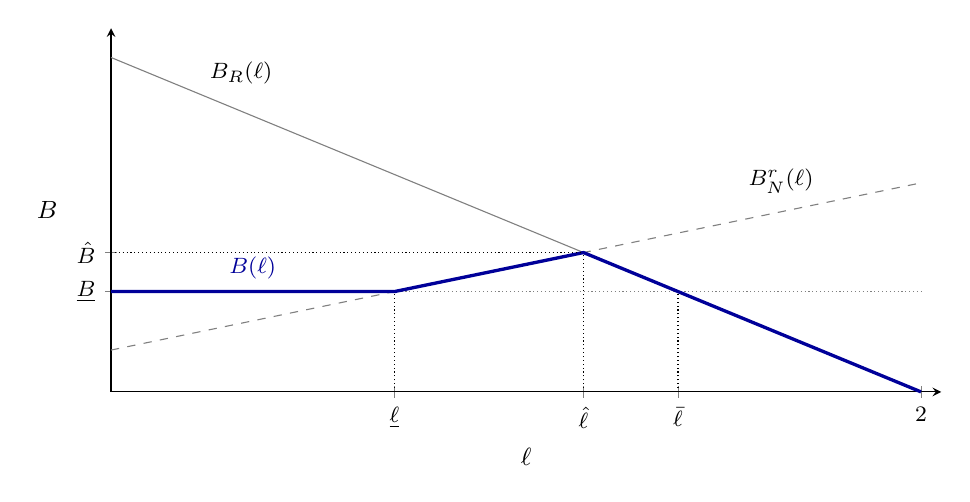
\begin{tikzpicture}
\begin{axis}[
  width=\linewidth, height=6.2cm,
  axis lines=left, xmin=0, xmax=2.05, ymin=0, ymax=1.45,
  xlabel={$\ell$}, ylabel={$B$}, ylabel style={rotate=-90},
  xtick={0.7,1.16667,1.4,2}, xticklabels={$\underline\ell$,$\hat\ell$,$\bar\ell$,$2$},
  ytick={0.4,0.55556}, yticklabels={$\underline B$,$\hat B$},
  tick label style={font=\footnotesize}, label style={font=\small},
  clip=false]
\addplot[domain=0:2, samples=2, dashed, gray] {1/6 + x/3};
\addplot[domain=0:2, samples=2, gray] {4/3 - 2*x/3};
\addplot[domain=0:2, samples=2, densely dotted, gray] {0.4};
\addplot[very thick, blue!60!black] coordinates {(0,0.4) (0.7,0.4) (1.16667,0.55556) (2,0)};
\draw[densely dotted] (axis cs:0.7,0) -- (axis cs:0.7,0.4);
\draw[densely dotted] (axis cs:1.16667,0) -- (axis cs:1.16667,0.55556);
\draw[densely dotted] (axis cs:1.4,0) -- (axis cs:1.4,0.4);
\draw[densely dotted] (axis cs:0,0.55556) -- (axis cs:1.16667,0.55556);
\node[font=\footnotesize, anchor=west] at (axis cs:1.55,0.84) {$B_N^r(\ell)$};
\node[font=\footnotesize, anchor=west] at (axis cs:0.22,1.27) {$B_R(\ell)$};
\node[font=\footnotesize, blue!60!black, anchor=south] at (axis cs:0.35,0.41) {$B(\ell)$};
\end{axis}
\end{tikzpicture}
\caption{The optimal amnesty rate}\label{fig:12-leniency-a}
\end{subfigure}\hfill
\begin{subfigure}[t]{0.49\textwidth}
\centering
\begin{tikzpicture}
\begin{axis}[
  width=\linewidth, height=6.2cm,
  axis lines=left, xmin=0, xmax=2.05, ymin=0, ymax=1.45,
  xlabel={$\ell$}, ylabel={$B$}, ylabel style={rotate=-90},
  xtick={1,1.16667}, xticklabels={$\hat\ell'$,$\hat\ell$},
  ytick={0.55556,0.66667}, yticklabels={$\hat B$,$\hat B'$},
  tick label style={font=\footnotesize}, label style={font=\small},
  clip=false]
\addplot[domain=0:2, samples=2, dashed, gray] {1/6 + x/3};
\addplot[domain=0:2, samples=2, thick, dashed, red!70!black] {1/3 + x/3};
\addplot[domain=0:2, samples=2, gray] {4/3 - 2*x/3};
\draw[densely dotted] (axis cs:1,0) -- (axis cs:1,0.66667) -- (axis cs:0,0.66667);
\draw[densely dotted] (axis cs:1.16667,0) -- (axis cs:1.16667,0.55556) -- (axis cs:0,0.55556);
\draw[-{Stealth[length=2mm]}] (axis cs:1.62,0.72) -- (axis cs:1.47,0.86);
\node[font=\footnotesize, anchor=west] at (axis cs:1.62,0.68) {$B_N^r(\ell;\varrho)$};
\node[font=\footnotesize, red!70!black, anchor=east] at (axis cs:1.45,0.92) {$B_N^r(\ell;\varrho')$};
\node[font=\footnotesize, anchor=west] at (axis cs:0.22,1.27) {$B_R(\ell)$};
\end{axis}
\end{tikzpicture}
\caption{A higher detection probability}\label{fig:12-leniency-b}
\end{subfigure}
\caption{Optimal leniency in the model of \citet{ChenRey2013}, drawn for $\delta = 0.8$ and $F = 1$. Panel (a): with
$\varrho = 0.3$, normal collusion survives above $\max\{\underline B, B_N^r(\ell)\}$ and collude and report survives
above $B_R(\ell)$. The deterrence threshold $B(\ell)$ (thick line) is the lower envelope. It equals
$\underline B = 0.4$ up to $\underline\ell = 0.7$ and peaks at $\hat\ell = \frac{7}{6}$, where
$\hat B = \frac{5}{9}$. Excessive leniency starts at $\bar\ell = 1.4$. Panel (b): raising $\varrho$ from 0.3 to
$\varrho' = 0.4$ shifts $B_N^r$ up and leaves $B_R$ unchanged, so the optimal rate falls to $\hat\ell' = 1$ and the
threshold rises to $\hat B' = \frac{2}{3}$. Redrawn with computed values from \citet{ChenRey2013}, Figures 1 and 2.}
\label{fig:12-leniency}
\end{figure}

\casehead{Interpretation}
\Cref{fig:12-leniency} shows the trade-off. Rates below $\underline\ell$ do nothing, because a deviator would not
report. Rates between $\underline\ell$ and $\hat\ell$ deter normal collusion in more industries, because they make
``cheat and report'' attractive. Rates above $\hat\ell$ hand the cartel a cheaper way to collude, by reporting itself
every period. At $\hat\ell$ the \emph{marginal industry}, with $B = \hat B$, is on the edge of both forms of
collusion. A lower rate would let it collude normally without fear of a reporting deviator. A higher rate would let it
collude and report without fear of a product-market deviator. Chen and Rey describe the instruments as a stick, the
probability $\varrho$ of random detection, and a carrot, the amnesty rate $\ell$. The weaker the stick, the larger
the optimal carrot. With no stick at all ($\varrho = 0$), $\underline\ell = 1$, so a pure fine reduction ($\ell \le 1$)
is useless and only rewards can work \citep[footnote~13]{ChenRey2013}.

Part~(d) of \cref{prop:12-chen-rey} explains why ``collude and report'' is rarely observed even though it is the
constraint that pins down the optimal rate. At the optimal rate, every industry that can collude prefers normal
collusion. The threat of self-reporting cartels shapes the policy without appearing in the data.

\begin{example}[Leniency with numbers]\label{ex:12-leniency-numbers}
Let $\delta = 0.8$, $\varrho = 0.3$ and $F = 1$, as in \cref{fig:12-leniency-a}. Without leniency,
$\underline B = \frac{0.8 \times 0.3}{0.6} = 0.4$. Deviators report once $\ell > 0.7$, and leniency becomes excessive
at $\bar\ell = 1.4$. The optimal rate is $\hat\ell = \frac{0.7}{0.6} = \frac{7}{6}$. The first informant thus pays no
fine and receives a reward of $\frac{1}{6}$ of the fine. The deterrence threshold rises to
$\hat B = \frac{0.8 \times 0.5}{0.6 \times 1.2} = \frac{5}{9} \approx 0.556$. Leniency extends deterrence from
industries with stakes below $0.4F$ to industries with stakes below $0.556F$, a rise of about 39 percent. In
industries that still collude, normal collusion beats collude and report by $\frac{0.7}{1.2}F \approx 0.583F$ per
firm. These values are computed in \texttt{figures/ch12/src/chenrey\_check.py}.
\end{example}

\casehead{Laboratory evidence}
\citet{HinloopenSoetevent2008}, as described by \citet[p.~13]{ChenRey2013}, ran laboratory experiments with
$\varrho = 0.4$ and $\delta = 0.8$. The model then prescribes full amnesty, since $\hat\ell = \frac{1 - 0.4}{1 - 0.4} = 1$.
One treatment set the rate at this level. The other granted full amnesty to a sole reporter and a 90 percent
reduction to each firm when both reported \citep[footnote~14]{ChenRey2013}. Under collude and report each firm then
pays $0.1F = (1 - \frac{\ell}{2})F$, which corresponds to $\ell = 1.8$. Subjects never colluded and reported in the
first treatment. More than 70 percent of subjects did so in every period of the second treatment, as the model
predicts. Our own computation shows how generous the second treatment is. With $\varrho = 0.4$, excessive leniency
starts at $\bar\ell = 1.2$. At $\ell = 1.8$, $B_R = \frac{0.8 \times 0.1}{0.6}F \approx 0.133F$, far below
$\underline B = \frac{0.8 \times 0.4}{0.6}F \approx 0.533F$. The program would make collusion sustainable in industries
that enforcement without leniency deters.

\citet{Spagnolo2004} proposes to reward the first informant with the fines paid by the other cartel members, which
corresponds to $\ell = 2$ in this model. \citet[p.~13]{ChenRey2013} counsel caution, because $\hat\ell < \bar\ell < 2$.
Actual programs grant reductions of up to 100 percent and rarely pay rewards. By \cref{prop:12-chen-rey}, such rates
may lie below the optimum when random detection is weak ($\varrho < \frac{\delta}{2}$).

\begin{remark}[The first-informant rule]\label{rem:12-first-informant}
Suppose both informants receive the reduced fine. Normal collusion is unaffected, because a deviator reports alone.
Under collude and report, however, each firm now pays $(1-\ell)F$ for sure. Repeating the derivation of
\eqref{eq:12-cr-BR} with $(1-\ell)$ in place of $(1 - \frac{\ell}{2})$ gives
\begin{equation}\label{eq:12-cr-BRprime}
B_R'(\ell) = \frac{\delta(1-\ell)}{2\delta - 1}\,F < B_R(\ell).
\end{equation}
At $\ell = \underline\ell = 1 - \varrho$, $B_R'(\underline\ell) = \frac{\delta\varrho F}{2\delta-1} = \underline B$.
For $\ell > \underline\ell$, $B_R'(\ell) < \underline B \le B_N(\ell)$, so the threshold falls below $\underline B$.
For $\ell \le \underline\ell$, the threshold equals $\underline B$. Without the first-informant rule, leniency cannot
raise deterrence at all \citep[pp.~13--14]{ChenRey2013}. The authors suggest that this may explain why the U.S. program
achieved little before its 1993 revision. The point agrees with \citet{Spagnolo2004} and \citet{Harrington2008}.
\end{remark}

\casehead{Repeat offenders}
Some jurisdictions deny leniency to repeat offenders, which seems to block cartels that report every period. Chen and
Rey argue that the restriction backfires. Their argument omits a participation condition. With it the conclusion is
established only when random detection is strong enough.

\begin{proposition}[Once-only leniency, after \citealp{ChenRey2013}, Proposition~2]\label{prop:12-repeat-offenders}
Suppose each industry can obtain leniency only once, and let $\ell \ge 0$. The strategy ``report once and never
again'' is sustainable if and only if $B \ge \underline B$ and
\begin{equation}\label{eq:12-cr-BO}
B \ge B_O(\ell) \equiv \left[(1-\delta)\left(1 - \frac{\ell}{2}\right) + \delta\varrho\right]F .
\end{equation}
The second condition holds at every $B \ge \underline B$ if and only if
$\ell \ge \ell_O \equiv 2\left(1 - \frac{2\delta\varrho}{2\delta - 1}\right)$. If
$\varrho \ge \frac{2\delta - 1}{2\delta + 1}$, then $\ell_O \le \underline\ell$. At every amnesty rate, normal
collusion or report once is then sustainable whenever $B \ge \underline B$. In that case once-only leniency cannot
deter collusion in any industry that enforcement without leniency fails to deter.
\end{proposition}

\begin{proof}
Under ``report once,'' the firms collude in every period, both report in the first period, and nobody reports
afterwards. Each firm's value is
\begin{equation*}
V_O = B - \left(1 - \frac{\ell}{2}\right)F + \delta V_N
= B - \left(1 - \frac{\ell}{2}\right)F + \delta\,\frac{B - \varrho F}{1-\delta}.
\end{equation*}
After the first report, leniency is no longer available. Reporting then only exposes the reporter, so play continues
as normal collusion without leniency. By \cref{prop:12-fines}, it is sustainable if and only if $B \ge \underline B$.
In the first period, reporting is self-enforcing, as under collude and report. A product-market deviator still
reports and pays $(1 - \frac{\ell}{2})F$ in expectation. It earns $2B$ and nothing afterwards. The first-period
constraint is
\begin{align*}
B - \left(1 - \frac{\ell}{2}\right)F + \delta V_N &\ge 2B - \left(1 - \frac{\ell}{2}\right)F\\
\delta\,\frac{B - \varrho F}{1-\delta} &\ge B\\
(2\delta - 1)B &\ge \delta\varrho F,
\end{align*}
which is again $B \ge \underline B$. A firm can also refuse at stage~0 of the first period. No evidence then arises,
the firms compete, and the refusing firm earns zero from then on. Refusal is unprofitable if and only if $V_O \ge 0$.
Multiplying $V_O \ge 0$ by $1 - \delta$ gives $B \ge (1-\delta)(1 - \frac{\ell}{2})F + \delta\varrho F$, which is
\eqref{eq:12-cr-BO}.

For the second claim, \eqref{eq:12-cr-BO} holds at $B = \underline B$ if and only if
\begin{equation*}
(1-\delta)\left(1 - \frac{\ell}{2}\right) \le \frac{\delta\varrho}{2\delta - 1} - \delta\varrho
= \frac{2(1-\delta)\delta\varrho}{2\delta - 1},
\end{equation*}
that is $1 - \frac{\ell}{2} \le \frac{2\delta\varrho}{2\delta - 1}$, or $\ell \ge \ell_O$. Since $B_O$ does not
depend on $B$, the condition then holds at every $B \ge \underline B$. Next, $\ell_O \le \underline\ell = 1 - \varrho$
if and only if $1 + \varrho \le \frac{4\delta\varrho}{2\delta - 1}$, that is $2\delta - 1 \le (2\delta + 1)\varrho$.
Normal collusion is unaffected by the restriction, since it never uses leniency on the path. By
\eqref{eq:12-cr-BN} it is sustainable at every $B \ge \underline B$ when $\ell \le \underline\ell$. Report once covers
every $\ell \ge \ell_O$, and $\ell_O \le \underline\ell$ leaves no gap.
\end{proof}

Chen and Rey check only the product-market constraints of report once, and their Proposition~2 states that the
restriction makes leniency ineffective without qualification \citep[pp.~14--15]{ChenRey2013}. The stage-0 refusal
matters. With $\delta = 0.8$, $\varrho = 0.3$, $F = 1$, $\ell = 0.2$ and $B = \underline B = 0.4$, we get
$V_N = 0.5$ and $V_O = 0.4 - 0.9 + 0.4 = -0.1 < 0$, so report once fails. Normal collusion survives there, because
$\ell = 0.2$ lies below $\underline\ell = 0.7$. In this example $\ell_O = 0.4 < \underline\ell$, and the
conclusion of Chen and Rey holds. When random detection is weak, both strategies can fail at a stake above
$\underline B$. With $\delta = 0.9$ and
$\varrho = 0.1$, $\underline\ell = 0.9$ and $\ell_O = 1.55$. At $\ell = 1.2$ and $B = 0.12F$, above
$\underline B = 0.1125F$, normal collusion needs $B \ge B_N^r(1.2) = 0.15F$ and report once needs
$B \ge B_O(1.2) = 0.13F$. Both fail. These values are our own computations in
\texttt{figures/ch12/src/chenrey\_check.py}. We have not shown that every other collusive strategy fails there too.

The logic of the proposition is that one report uses up the industry's access to leniency. Afterwards no member can
gain from reporting, which removes the threat that made normal collusion fragile. The first report is costly,
however, and a cartel accepts that cost only if the whole path is worth at least the zero it earns by not forming.
Chen and Rey quote \citet{Wils2008} on the same
paradox, that excluding recidivists from leniency may encourage recidivism. When exposed cartels face closer scrutiny
afterwards, excluding repeat offenders still weakens the program but no longer makes it useless
\citep[p.~17]{ChenRey2013}.

\casehead{Closer scrutiny after exposure}
So far an exposed cartel could collude again in the next period. Suppose instead that an exposed industry is kept
under tight supervision for $T$ periods, during which it cannot collude. Define
\begin{equation}\label{eq:12-cr-beta-gamma}
\beta_T \equiv \delta^{T+1}, \qquad \gamma_T \equiv (1-\varrho)\delta + \varrho\beta_T,
\end{equation}
so that $\beta_T < \gamma_T < \delta$ for $T \ge 1$. (Chen and Rey write $\beta(T)$ and $\gamma(T)$.) A cartel that
reports every period is exposed every period, so its future is discounted at $\beta_T$:
\begin{equation*}
V_R(\ell;T) = B - \left(1 - \frac{\ell}{2}\right)F + \beta_T V_R(\ell;T)
\quad\Longrightarrow\quad
V_R(\ell;T) = \frac{B - \left(1 - \frac{\ell}{2}\right)F}{1 - \beta_T}.
\end{equation*}
A normal cartel is exposed only with probability $\varrho$:
\begin{equation*}
V_N(T) = B - \varrho F + (1-\varrho)\delta V_N(T) + \varrho\beta_T V_N(T)
\quad\Longrightarrow\quad
V_N(T) = \frac{B - \varrho F}{1 - \gamma_T}.
\end{equation*}
Repeating the derivations of \eqref{eq:12-fines-threshold}, \eqref{eq:12-cr-BNr} and \eqref{eq:12-cr-BR} with these
values gives
\begin{equation}\label{eq:12-cr-scrutiny}
\underline B(T) = \frac{\gamma_T\varrho F}{2\gamma_T - 1},\qquad
B_N^r(\ell;T) = \frac{\varrho - (1-\gamma_T)(1-\ell)}{2\gamma_T - 1}\,F,\qquad
B_R(\ell;T) = \frac{\beta_T\left(1 - \frac{\ell}{2}\right)}{2\beta_T - 1}\,F.
\end{equation}
The last expression requires $\beta_T > \frac{1}{2}$.\footnote{Footnote~20 of the working paper (p.~16) prints this
assumption as $\beta(T) < \frac{1}{2}$. That inequality contradicts the paper's own formula for $B_R(q;T)$, whose
denominator $2\beta(T) - 1$ must be positive. It also contradicts the footnote's own parenthetical remark, which
treats $\gamma(T) > \frac{1}{2} > \beta(T)$ as the case in which collude and report cannot be sustained. We state the
condition that the formula needs.} If $\beta_T \le \frac{1}{2}$ and $\ell < 2$, collude and report
cannot be sustained at any stake. The authority can then raise the amnesty rate up to that bound without inviting
self-reporting cartels.
Equating $B_N^r(\ell;T)$ and $B_R(\ell;T)$ gives the optimal rate
\begin{equation}\label{eq:12-cr-qhatT}
\hat\ell(T) = \frac{2(1-\varrho)(\beta_T + \delta - 1)}{(2\beta_T - 1) + (2\gamma_T - 1)(1 - \beta_T)},
\end{equation}
which reduces to \eqref{eq:12-cr-qhat} at $T = 0$, where $\beta_0 = \gamma_0 = \delta$.

\begin{proposition}[Scrutiny, \citealp{ChenRey2013}, Proposition~3]\label{prop:12-scrutiny}
Assume $\beta_T > \frac{1}{2}$. A longer period $T$ of close scrutiny for exposed cartels raises the maximal
deterrence threshold $\hat B(T)$ and also raises the optimal amnesty rate $\hat\ell(T)$.
\end{proposition}

Scrutiny lowers the value of both forms of collusion, but it hurts collude and report more, because that cartel is
exposed in every period. The authority can then offer more amnesty without inviting self-reporting cartels. With
$\delta = 0.9$ and $\varrho = 0.2$, for instance, our computations give $\hat\ell = 1.455$ and $\hat B = 0.307F$ at
$T = 0$, $\hat\ell = 1.534$ and $\hat B = 0.371F$ at $T = 2$, and $\hat\ell = 1.873$ and $\hat B = 0.539F$ at
$T = 5$. At $T = 6$, $\beta_T = 0.9^7 < \frac{1}{2}$, and collude and report is no longer sustainable.

\begin{remark}[More than two firms]\label{rem:12-cr-nfirms}
The model extends directly to $N$ firms, an extension we derive here. A deviator earns $NB$, and under collude and
report each firm is the first informant with probability $\frac{1}{N}$, so its expected fine is
$(1 - \frac{\ell}{N})F$. The derivations above give
\begin{equation*}
B_N^r(\ell) = \frac{\varrho - (1-\delta)(1-\ell)}{N\delta - (N-1)}\,F,\qquad
B_R(\ell) = \frac{\delta\left(1 - \frac{\ell}{N}\right)}{N\delta - (N-1)}\,F,
\end{equation*}
and the optimal rate solves $\varrho - (1-\delta) + (1-\delta)\ell = \delta - \frac{\delta\ell}{N}$, so
\begin{equation*}
\hat\ell_N = \frac{1 - \varrho}{1 - \frac{N-1}{N}\delta},\qquad
\hat B_N = \frac{\delta[(N-1)(1-\delta) + \varrho]}{[N\delta - (N-1)][N(1-\delta) + \delta]}\,F.
\end{equation*}
Excessive leniency starts at $\bar\ell_N = N(1-\varrho)$. Both $\hat\ell_N$ and $\bar\ell_N$ rise with $N$. A reporting
cartel with many members spreads the amnesty thinly, so the authority can afford a larger reward. With $\delta = 0.9$
and $\varrho = 0.3$, $\hat\ell_N$ equals 1.27, 1.75 and 2.15 for $N = 2$, 3 and 4. This extension keeps the restriction
to the two strategies N and R.
\end{remark}

\casehead{Leniency before and after an investigation}
The final part of \citet[Section~4]{ChenRey2013} separates the launch of an investigation from its outcome. Absent any
report, the authority opens an investigation with probability $\iota \in (0,1)$. An open investigation uncovers the
cartel, absent any report, with probability $\varsigma \in (0,1)$. (Chen and Rey write $\alpha$ and $p$.) Both
probabilities are likely to be small in practice. If investigations are secret, firms face the overall detection
probability $\varrho = \iota\varsigma$, and \cref{prop:12-chen-rey} applies with this $\varrho$. If the rates before
and after an investigation differ, the relevant secret rate is the expected one, $\iota\ell_a + (1-\iota)\ell_b$
\citep[footnote~22]{ChenRey2013}.

If investigations are public, the authority can set two rates. A first informant pays $(1-\ell_b)F$ if it reports
before an investigation and $(1-\ell_a)F$ if it reports after one has opened. Stages~0 to~2 are as before. At
stage~3, if nobody has reported, the authority opens an investigation with probability $\iota$. At stage~4 the firms
may report again, and an unreported cartel under investigation is uncovered with probability $\varsigma$. Public investigations create a third collusive strategy, \emph{collude and report if
investigated} (I).

The authority can always do as well with public investigations as with secret ones, by setting $\ell_a = 0$. A report
after an investigation then raises the probability of conviction from $\varsigma$ to 1 without reducing the fine, so
nobody reports at stage~4. The choice between N and R is then the same as with secret investigations. The question is
whether $\ell_a > 0$ can do strictly better.

Each strategy faces several deviations, and we derive each threshold from a comparison of values. Normal collusion now
has value $V_N = \frac{B - \iota\varsigma F}{1-\delta}$. It must deter four deviations. Deviating without reporting
gives $\underline B = \frac{\delta\iota\varsigma F}{2\delta - 1}$. Deviating and reporting at stage~2 gives
$B_N^r(\ell_b) = \frac{\iota\varsigma - (1-\delta)(1-\ell_b)}{2\delta - 1}F$. Deviating and reporting only if
investigated yields $2B - \iota(1-\ell_a)F$, and $V_N \ge 2B - \iota(1-\ell_a)F$ gives
\begin{equation*}
B \ge B_N^i(\ell_a) \equiv \frac{\iota\varsigma - \iota(1-\delta)(1-\ell_a)}{2\delta - 1}\,F.
\end{equation*}
Colluding but reporting once an investigation opens compares $-\varsigma F + \delta V_N$ (stay silent and keep the
cartel) with $-(1-\ell_a)F$ (report and lose it). Staying silent is better if and only if
\begin{equation*}
B \ge B_N^c(\ell_a) \equiv \frac{\varsigma(1 - \delta + \iota\delta) - (1-\delta)(1-\ell_a)}{\delta}\,F.
\end{equation*}
Normal collusion is therefore sustainable if and only if
\begin{equation}\label{eq:12-cr-open-N}
B \ge B_N(\ell_b, \ell_a) \equiv \max\{B_N^i(\ell_a),\, B_N^r(\ell_b),\, B_N^c(\ell_a),\, \underline B\},
\end{equation}
equation~(6) of \citet{ChenRey2013}. Collude and report is sustainable if and only if
$B \ge B_R(\ell_b) = \frac{\delta(1 - \frac{\ell_b}{2})F}{2\delta-1}$, as before. Under collude and report if
investigated, each firm pays $(1 - \frac{\ell_a}{2})F$ when an investigation opens, so
$V_I = \frac{B - \iota(1 - \frac{\ell_a}{2})F}{1-\delta}$. Reporting when investigated is self-enforcing, since it cuts
the expected fine from $F$ to $(1 - \frac{\ell_a}{2})F$ when the rival reports. Strategy I must deter a deviation with
a report at stage~2, which yields $2B - (1-\ell_b)F$, and a deviation with a report only if investigated, which yields
$2B - \iota(1 - \frac{\ell_a}{2})F$. These give
\begin{equation}\label{eq:12-cr-open-I}
B \ge B_I(\ell_b, \ell_a) \equiv \max\left\{
\frac{\delta\iota\left(1 - \frac{\ell_a}{2}\right)}{2\delta - 1}\,F,\;
\frac{\iota\left(1 - \frac{\ell_a}{2}\right) - (1-\delta)(1-\ell_b)}{2\delta - 1}\,F\right\},
\end{equation}
where the two terms are $B_I^i(\ell_a)$ and $B_I^r(\ell_b, \ell_a)$, equation~(7) of \citet{ChenRey2013}. The
authority maximizes $\min\{B_N(\ell_b,\ell_a),\, B_I(\ell_b,\ell_a),\, B_R(\ell_b)\}$. Without post-investigation
leniency, the optimum is $\ell_b = \hat\ell(\iota\varsigma)$ with threshold $\hat B(\iota\varsigma)$, from
\eqref{eq:12-cr-qhat} and \eqref{eq:12-cr-Bhat}.

Post-investigation leniency can destabilize normal collusion in two ways. The first route makes ``deviate and report
if investigated'' the binding deviation. This requires $B_N^i(\ell_a) > B_N^r(\hat\ell_b)$, that is,
$\iota(1-\ell_a) < 1 - \hat\ell(\iota\varsigma)$. It must not make strategy I more robust, which requires
$B_I^r(\hat\ell_b, \ell_a) > B_N^r(\hat\ell_b)$, that is, $\varsigma < 1 - \frac{\ell_a}{2}$. Both conditions hold for
some $\ell_a$ if and only if
\begin{equation}\label{eq:12-cr-p1}
\varsigma < \tilde\varsigma_1(\iota) \equiv \frac{\iota(2-\delta) - \delta}{2\iota(1-\delta)},
\end{equation}
equation~(9) of \citet{ChenRey2013}. To verify it, substitute $1 - \hat\ell(\iota\varsigma) =
\frac{2\iota\varsigma - \delta}{2-\delta}$ into the first condition and combine it with $\ell_a < 2(1-\varsigma)$.
Then reduce $\ell_b$ slightly below $\hat\ell$ to raise $B_R$ as well. The best policy of this kind equalizes the three
binding thresholds, $B_N^i(\tilde\ell_a^1) = B_I^r(\tilde\ell_b^1, \tilde\ell_a^1) = B_R(\tilde\ell_b^1)$, which gives
\begin{equation}\label{eq:12-cr-policy1}
\tilde\ell_b^1 = \frac{2[(1-\iota)(2-\delta) + \iota(1-\varsigma)]}{2(1-\delta)^2 + 2 - \delta},\qquad
\tilde\ell_a^1 = \frac{2}{\iota}\cdot\frac{\delta(1-\delta)(1-\iota) + \iota(1-\varsigma)(2-\delta)}{2(1-\delta)^2 + 2 - \delta},
\end{equation}
and the deterrence threshold
\begin{equation}\label{eq:12-cr-B1}
\tilde B_1 = \frac{2(1-\delta)^2 + \iota(1 - \delta + \varsigma)}{2(1-\delta)^2 + 2 - \delta}\cdot\frac{\delta F}{2\delta - 1},
\end{equation}
equations~(10) and~(11) of \citet{ChenRey2013}. It exceeds $\hat B(\iota\varsigma)$ if and only if
$\varsigma \le \tilde\varsigma_1(\iota)$. The second route makes ``collude but report if investigated'' the binding
deviation. It is available if and only if
\begin{equation}\label{eq:12-cr-p2}
\varsigma \le \tilde\varsigma_2(\iota) \equiv \frac{(1-\delta)(3\delta - 2)}{(2\delta - 1)(2-\delta) + 2\iota\delta(1-\delta)},
\end{equation}
which is positive only when $\delta > \frac{2}{3}$. Its best version $(\tilde\ell_b^2, \tilde\ell_a^2)$ equalizes
$B_N^c$, $B_I^r$ and $B_R$, with threshold
\begin{equation}\label{eq:12-cr-B2}
\tilde B_2 = \frac{2(1-\delta)^2 + \iota(1-\delta) + (1 - \delta + \iota\delta)\iota\varsigma}
{2(2\delta - 1)(1-\delta)(2-\delta) + \iota\delta^2}\,\delta F,
\end{equation}
equations~(12) to~(14) of \citet{ChenRey2013}. The first route beats the second if and only if
$\varsigma \ge \tilde\varsigma(\iota)$, where
\begin{equation}\label{eq:12-cr-ptilde}
\tilde\varsigma(\iota) \equiv \frac{2(1-\delta)(2\delta - 1) + \iota(2\delta^2 - 1) - \iota^2\delta}
{\iota(2\delta - 1)(3 - 2\delta) + 4\iota^2(1-\delta)^2},
\end{equation}
which is nonpositive for $\iota \ge \iota_1 \equiv \frac{2\delta - 1}{\delta}$. We checked every formula in this
paragraph symbolically in \texttt{chenrey\_check.py}.

\begin{proposition}[Pre- and post-investigation leniency, \citealp{ChenRey2013}, Proposition~4]\label{prop:12-cr-open}
It is always optimal to offer leniency before an investigation.
\begin{enumerate}[label=(\alph*)]
\item If firms are patient ($\delta > \frac{2}{3}$), it is optimal to keep offering some leniency once an investigation
is under way if and only if $\varsigma \le \max\{\tilde\varsigma_1(\iota), \tilde\varsigma_2(\iota)\}$. The optimal
policy is then $(\tilde\ell_b^1, \tilde\ell_a^1)$ if $\varsigma \ge \tilde\varsigma(\iota)$ and
$(\tilde\ell_b^2, \tilde\ell_a^2)$ if $\varsigma \le \tilde\varsigma(\iota)$.
\item If firms are less patient ($\frac{1}{2} < \delta \le \frac{2}{3}$), it is optimal to keep offering some leniency
once an investigation is under way if and only if $\iota \ge \underline\iota \equiv \frac{\delta}{2-\delta}$ and
$\varsigma \le \tilde\varsigma_1(\iota)$. The optimal policy is then $(\tilde\ell_b^1, \tilde\ell_a^1)$.
\end{enumerate}
In all other cases the optimal policy is $(\hat\ell(\iota\varsigma), 0)$.
\end{proposition}

\begin{figure}[htbp]
\centering
\begin{subfigure}[t]{0.49\textwidth}
\centering
\begin{tikzpicture}
\begin{axis}[
  width=\linewidth, height=6cm,
  axis lines=left, xmin=0, xmax=1.03, ymin=0, ymax=1.03,
  xlabel={$\iota$}, ylabel={$\varsigma$}, ylabel style={rotate=-90},
  xtick={0,0.666667,1}, xticklabels={$0$,$\frac{2}{3}$,$1$},
  ytick={0,0.2,1}, yticklabels={$0$,$0.2$,$1$},
  tick label style={font=\footnotesize}, label style={font=\small},
  clip=false]
\addplot[thick, domain=0:0.686141, samples=60] {1/(9+4*x)};
\addplot[thick, domain=0.686141:1, samples=120] {3-2/x};
\addplot[thick, dashed, domain=0.686141:0.75, samples=60] {(6+7*x-20*x^2)/(21*x+4*x^2)};
\draw[densely dotted, gray] (axis cs:0,0.2) -- (axis cs:1,0.2);
\node[font=\small] at (axis cs:0.40,0.55) {A};
\node[font=\small] at (axis cs:0.92,0.30) {B};
\node[font=\footnotesize, anchor=east] at (axis cs:0.86,0.75) {$\tilde\varsigma_1(\iota)$};
\node[font=\footnotesize, anchor=south west] at (axis cs:0.04,0.115) {$\tilde\varsigma_2(\iota)$};
\end{axis}
\end{tikzpicture}
\caption{The unit square}\label{fig:12-leniency-regions-a}
\end{subfigure}\hfill
\begin{subfigure}[t]{0.49\textwidth}
\centering
\begin{tikzpicture}
\begin{axis}[
  width=\linewidth, height=6cm,
  axis lines=left, xmin=0, xmax=1.03, ymin=0, ymax=0.206,
  xlabel={$\iota$}, ylabel={$\varsigma$}, ylabel style={rotate=-90},
  xtick={0,0.666667,0.75,1}, xticklabels={$0$,$\frac{2}{3}$,$\frac{3}{4}$,$1$},
  ytick={0,0.085,0.111111,0.2}, yticklabels={$0$,$\varsigma_0$,$\frac{1}{9}$,$0.2$},
  tick label style={font=\footnotesize}, label style={font=\small},
  clip=false]
\addplot[thick, domain=0:0.686141, samples=60] {1/(9+4*x)};
\addplot[thick, domain=0.686141:0.714286, samples=60] {3-2/x};
\addplot[thick, dashed, domain=0.686141:0.75, samples=60] {(6+7*x-20*x^2)/(21*x+4*x^2)};
\draw[densely dotted] (axis cs:0,0.085) -- (axis cs:0.686,0.085);
\node[font=\small] at (axis cs:0.35,0.165) {A};
\node[font=\small] at (axis cs:0.88,0.10) {B};
\node[font=\small] at (axis cs:0.35,0.045) {C};
\node[font=\footnotesize, anchor=east] at (axis cs:0.69,0.18) {$\tilde\varsigma_1(\iota)$};
\node[font=\footnotesize, anchor=south] at (axis cs:0.30,0.104) {$\tilde\varsigma_2(\iota)$};
\node[font=\footnotesize, anchor=west] at (axis cs:0.76,0.055) {$\tilde\varsigma(\iota)$};
\draw[-{Stealth[length=1.5mm]}] (axis cs:0.765,0.05) -- (axis cs:0.73,0.03);
\end{axis}
\end{tikzpicture}
\caption{Detail for $\varsigma \le 0.2$}\label{fig:12-leniency-regions-b}
\end{subfigure}
\caption{Optimal leniency policies with public investigations for $\delta = 0.8$, computed from
\eqref{eq:12-cr-p1}, \eqref{eq:12-cr-p2} and \eqref{eq:12-cr-ptilde}. The horizontal axis is the probability $\iota$
that an investigation opens, and the vertical axis the probability $\varsigma$ that it succeeds without a report.
Here $\tilde\varsigma_1(\iota) = 3 - \frac{2}{\iota}$ and $\tilde\varsigma_2(\iota) = \frac{1}{9 + 4\iota}$, and the
three curves meet at $\iota_0 \approx 0.686$, $\varsigma_0 \approx 0.085$. In region A no leniency is offered after an
investigation opens. In region B the optimal policy is $(\tilde\ell_b^1, \tilde\ell_a^1)$, and in region C it is
$(\tilde\ell_b^2, \tilde\ell_a^2)$. Panel (b) enlarges the strip $\varsigma \le 0.2$ of panel (a). Redrawn with
computed boundaries from \citet{ChenRey2013}, Figure~4.}
\label{fig:12-leniency-regions}
\end{figure}

\Cref{fig:12-leniency-regions} draws the regions for $\delta = 0.8$. Post-investigation leniency pays when an
investigation, once opened, is unlikely to succeed without a report. It also needs investigations to be frequent
enough for the threat of one to matter at the margin. If deviations in the product market are detected quickly, a
deviator cannot wait for an investigation before reporting. Then only the second route remains, and
post-investigation leniency is optimal if and only if $\varsigma \le \tilde\varsigma_2(\iota)$
\citep[footnote~26]{ChenRey2013}.

\begin{proposition}[Comparative statics, \citealp{ChenRey2013}, Propositions~5 and~6]\label{prop:12-cr-statics}
\leavevmode
\begin{enumerate}[label=(\alph*)]
\item A higher $\varsigma$ or a higher $\iota$ makes the leniency program more effective.
\item A higher $\varsigma$ calls for less leniency both before and after an investigation.
\item A higher $\iota$ calls for less leniency before an investigation. The post-investigation rate $\tilde\ell_a^1$
falls with $\iota$, while $\tilde\ell_a^2$ rises with $\iota$.
\item Offering post-investigation leniency lowers the pre-investigation rate: $\tilde\ell_b^1 < \hat\ell$ and
$\tilde\ell_b^2 < \hat\ell$.
\item More leniency is offered after than before an investigation when investigations are unlikely to succeed:
$\tilde\ell_b^1 < \tilde\ell_a^1$ if and only if $\varsigma < \hat\varsigma_1(\iota)$, and $\tilde\ell_b^2 <
\tilde\ell_a^2$ if and only if $\varsigma < \hat\varsigma_2(\iota)$, where
\begin{equation*}
\hat\varsigma_1(\iota) = (1-\delta)\,\frac{\iota^2 + \delta(1-\iota)}{\iota(2 - \delta - \iota)},\qquad
\hat\varsigma_2(\iota) = \frac{1-\delta}{2\delta - 1}\cdot\frac{\delta(1-\delta) + \iota(2\delta - 1)}{(1 - \delta + \iota\delta)(2 - \delta - \iota)}.
\end{equation*}
\end{enumerate}
\end{proposition}

Part~(d) has a simple logic. Without post-investigation leniency, the marginal industry is on the edge of both normal
collusion and collude and report. Post-investigation leniency destabilizes normal collusion further, and the
pre-investigation rate must then fall to keep collude and report in check. Part~(e) speaks to actual programs. The U.S.
program offers complete amnesty to the first qualifying informant whether or not an investigation is under way, with
further conditions once one has begun. The EU's 1996 notice granted 75 to 100 percent before an investigation and only
50 to 75 percent after. Neither offered more leniency after an investigation opened. \citet[p.~29]{ChenRey2013} conclude that such policies may not be optimal when investigations
rarely succeed without a report.

\casehead{Interpretation}
The model gives sharp answers to the policy questions of \cref{sec:12-legal}. Some leniency always helps, and the
optimal amount falls as random detection improves. Leniency should go to the first informant only. Excluding repeat
offenders can disable the program, at least when random detection is not too weak. Leniency after an investigation opens is valuable when investigations alone rarely
uncover cartels, which is the realistic case. In repeated-game terms, leniency adds the deviation ``cheat and
report'' to the incentive constraint, and its generosity is limited by a second constraint for cartels that report
themselves.

\casehead{Critiques and limitations}
The model is deliberately stark, and several of its simplifications matter.
\begin{enumerate}[label=(\arabic*)]
\item Conduct is binary. With a continuum of collusive prices, leniency would also change the price that a cartel
sets, as \citet[footnote~7]{ChenRey2013} acknowledge.
\item Evidence lasts one period, so a cartel cannot be prosecuted for past conduct. Real fines grow with the duration
of the infringement, and past evidence accumulates. Detection risk then changes over time, which creates a ``race to
the courthouse'' when an investigation looms. \citet{Harrington2008} models this race. With a detection probability
that changes stochastically over time, leniency has two opposing effects \citep[p.~209]{AskerNocke2021}. The
\emph{deviator amnesty effect} lets a member that has just undercut its rivals also report the cartel and escape the
fine, which tightens the no-cheating constraint. The \emph{cartel amnesty effect} lowers the expected fines that
members pay, which raises the value of colluding. A more lenient program can also trigger a switch from no firm
applying to all firms racing to apply, which raises expected fines.
\item The probabilities $\varrho$, $\iota$ and $\varsigma$ are exogenous. Reports free investigative resources, and
\citet{MottaPolo2003} study how an authority allocates a budget between investigation and prosecution. Detection may
also depend on conduct, since price wars and abrupt price rises draw attention.
\item Firms are symmetric. A member that plans to exit, or one with little to lose, has a stronger motive to report.
Asker's weak ring members (\cref{sec:13-asker}) illustrate how asymmetries shape the threat of reporting.
\item Only firms are sanctioned and rewarded. \citet{AubertReyKovacic2006} argue that rewards to individual employees
can deter more effectively. Prison terms for executives make schemes of taking turns at reporting unattractive, as
Wils notes in the passage quoted by \citet[p.~2]{ChenRey2013}.
\item The evidence is mostly experimental. Field evaluation is hard, because the number of detected cartels rises both
when leniency destabilizes cartels and when more cartels form or report themselves. \citet{HarringtonChang2009} build
a model of cartel birth and death to evaluate policy from detected cartels, and \cref{prop:13-selection} shows how
detection shapes the cartels we observe.
\end{enumerate}

\casehead{Contribution}
\citet{ChenRey2013} turn an informal worry into a tractable design problem. The optimal amnesty rate balances two
incentive constraints, one for cartels that fear a reporting deviator and one for cartels that report themselves. The
framework rationalizes the first-informant rule and post-investigation amnesty, the two innovations of the 1993 U.S.
revision. It also warns against generous rewards and against excluding repeat offenders.

\subsection{The agreement requirement: Kaplow (2013)}\label{sec:12-kaplow}

\citet{Kaplow2013} questions the legal foundation on which this enforcement rests. Under Section~1 of the Sherman Act
and Article~101, liability for price fixing requires an agreement among competitors. The conventional view
distinguishes \emph{pure interdependence}, in which firms refrain from price cutting because each expects
retaliation, from classic cartels, whose members meet in hotel rooms to discuss prices. It treats the first as
insufficient for liability and the second as more than sufficient (p.~4). Since the \textit{Theatre Enterprises} decision, courts
have held conscious parallelism by itself to be insufficient. A plaintiff must also show ``plus factors'', such as
actions contrary to the defendants' interests if taken independently and a motive to agree (pp.~109--110). On the
conventional view an agreement turns on the use of certain interfirm communications (p.~21). Kaplow argues that this
focus is misplaced. The harm from coordinated price elevation depends on the extent and duration of supracompetitive
pricing, not on the means used to reach or maintain the understanding (pp.~9--10). That harm is the same whether
firms coordinate in a hotel room or by reading one another's prices.

The repeated-game theory of this chapter supports the premise. In the perfect-monitoring supergames of
\cref{sec:12-perfect}, tacit and explicit collusion are the same equilibrium. The incentive constraint of
\cref{prop:12-bertrand} does not mention communication, and talk is cheap. If communication changes anything, it
selects among the many sustainable prices of \cref{cor:12-bertrand-any-price}.

A test based on communications is hard to state (ch.~3). In its ordinary meaning, communication is any exchange of
information through a common system of symbols, signs or behavior (p.~51). Price moves are behavior conveyed by
signs, so a rule triggered by any communication would cover all interdependent pricing (p.~52). A narrower rule must
count only some communications. It could limit them by mode, counting meetings and emails and excluding hand
signals. It could limit them by content, counting talk about future prices and excluding talk about current ones. Or
it could limit them by setting, counting hotel rooms and excluding public announcements. Modes of communication are close substitutes, however. A fixed list of forbidden modes invites
circumvention, and a rule that includes all functional equivalents covers every successful interdependence
(p.~53). Kaplow draws a striking conclusion. If liability requires certain communications, then ``truly naked price
fixing is per se legal,'' and illegality flows from the communications that clothe it (p.~61).

Noncooperative game theory has no word for agreement, but its central concept is close to the legal one
(pp.~196--199). Courts and dictionaries often define an agreement as a meeting of the minds. An equilibrium of a
repeated game is a mutual understanding about current prices and about the consequences of defection. In any
equilibrium each firm acts in its own interest, given what it expects its rivals to do. A nonbinding agreement that
is not in every member's interest is not honored, so it is not an equilibrium. In Kaplow's words, ``All nonbinding
agreements that work are equilibria, and all equilibria are nonbinding agreements that work'' (p.~197). Not every
equilibrium is objectionable. In repeated static play, no firm refrains from cutting its price because it expects
others to respond, so that equilibrium needs no meeting of the minds (pp.~197--198). Kaplow therefore reads
agreement as successful oligopolistic interdependence, the firms' mutual understanding that sustains
supracompetitive prices (pp.~198--199). On this reading the legal notion maps onto the most collusive equilibria of
\cref{sec:12-folk}.

Communications do not appear in the theory of oligopoly, yet they can matter in two ways (pp.~199--204). The first is
equilibrium selection. Without words, firms may settle on the monopoly price as a focal point, or they may not.
Negotiation helps when the firms disagree about the monopoly price because their costs or their views of demand
differ, and when they sell several products. It can also fail where simple price signaling would quickly converge on
a round number (pp.~200--201). The experimental evidence that Kaplow cites is mixed. In one coordination game,
players reached the good equilibrium 48 percent of the time without communication, 55 percent with two-way
communication and 95 percent with one-way communication (p.~201, note~54). The second role is enforcement when
prices are unobservable. Firms that infer cheating from their own sales risk accidental price wars, and credible
information can avoid them. Cheap talk about compliance is not credible, so verification, such as audits of
invoices, matters more than talk (pp.~202--203). Communication can also hurt a cartel. If firms expect to negotiate
an end to any price war, punishments become brief and cheating more attractive (p.~203). Kaplow concludes that
communications help explain coordinated pricing but do not illuminate the notion of agreement (p.~206). He reaches
the same conclusion about promises and assurances (pp.~206--214).

Kaplow points to what he calls the \emph{paradox of proof} (pp.~6--7 and ch.~6). It arises from two features of the
conventional rule. Agreement requires more than successful interdependence, for example the use of certain
communications. And because firms hide their communications, the factfinder must infer them from circumstantial
evidence, notably from how conducive market conditions are to coordination. Conditions such as few sellers,
homogeneous products and transparent prices make successful price elevation more likely. Beyond some point, they
also make it more likely that firms coordinated without the prohibited means of communication. Evidence of a
greater danger of coordinated pricing can thus reduce the likelihood that an agreement, in the legal sense, exists
(p.~7). A rule that turns on communication tends to exonerate the industries where collusion is most likely.

A stylized calculation of our own, not taken from Kaplow, makes the point concrete. Consider a duopoly with stake
$B \ge \underline B$, so that collusion is sustainable with or without fines. Without communication its firms reach
the collusive equilibrium with probability $\zeta \in [0,1]$ and otherwise compete forever. The parameter $\zeta$
measures how easy tacit coordination is. With communication they always coordinate, but they
face the expected fine $\varrho F$ per period of \cref{sec:12-fines}. Firms communicate if and only if
\begin{equation}\label{eq:12-kaplow}
\frac{B - \varrho F}{1-\delta} > \frac{\zeta B}{1-\delta}
\iff \zeta < 1 - \frac{\varrho F}{B}.
\end{equation}
Industries where tacit coordination is easy collude silently and face no sanction. Industries where it is hard
communicate and are exposed to fines. Tougher enforcement of the agreement requirement lowers the cutoff in
\eqref{eq:12-kaplow}. The industries it moves switch from explicit to tacit collusion. They still collude with
probability $\zeta$, so enforcement deters collusion in them only with probability $1 - \zeta$. The sanction falls
where collusion would otherwise be least likely.

Kaplow proposes a \emph{direct approach}, in which liability turns on evidence that firms engaged in successful
coordinated price elevation, whatever the means (pp.~9--15). Such evidence includes price increases not matched
by changes in cost, price wars, markups estimated from prices and marginal costs or from demand elasticities, and
the conduciveness of market conditions (p.~11). Internal evidence, including interfirm communications, remains
relevant as one source of proof (p.~12). Liability and sanctions should be set by weighing deterrence benefits
against the chilling of desirable behavior and the costs of administration (p.~10). Kaplow argues that, if the
burden of proof under the direct approach is set to find liability in as many cases as the conventional rule, the
direct approach dominates. It targets cases with greater social danger and a lower risk of chilling (p.~14). The
debate is old. \citet{Turner1962} accepted that interdependence could count as agreement as a matter of statutory
language, but rejected it as a basis for liability as a matter of policy. \citet{Posner1969} first argued that this
policy analysis was unsound \citep[p.~447]{Kaplow2013}.

The theory of this chapter gives precise content to Kaplow's second role and so gives reasons to treat
communication as more than a proxy. When information is private, communication changes what can be sustained. In the
model of \citet{HarringtonSkrzypacz2011}
(\cref{thm:12-hs}), sales reports and transfers make collusion possible when unobserved prices would otherwise
undermine it. Without communication, the optimal scheme of \citet{AtheyBagwellSanchirico2004} uses rigid prices and
gives up productive efficiency (\cref{sec:12-private-costs}). With communication about costs, \citet{AtheyBagwell2001}
show that cartels can do better. Explicit agreements may thus raise prices in markets where tacit coordination would
fail. An outcome-based rule faces a measurement problem as well. It must show that prices exceed a noncooperative
benchmark, the identification problem of \cref{ch:conduct}. Conduct that varies with demand, as in the Corts critique
\citep{Corts1999}, makes that benchmark hard to estimate. The detection methods of \cref{ch:collusion-evidence} show
both what such evidence can achieve and how often it is ambiguous.

\section{What Determines Cartel Success?}\label{sec:12-success}

Theory tells us which collusive outcomes can be sustained. It does not tell us how often cartels form, how long they
last, or why they end. \citet{LevensteinSuslow2006} survey the empirical studies of explicit cartels to answer four
questions (p.~43). Can cartels succeed? If so, for how long? What impact do they have? What causes them to break up?
Their survey combines cross-section studies of many cartels with nineteen case studies of individual industries. It is
the main bridge between the theory of this chapter and the evidence of \cref{ch:collusion-evidence}. Page references
are to the journal article.

\subsection{Theory and measurement}\label{sec:12-ls-measure}

\citet[p.~45]{LevensteinSuslow2006} organize the theory around three problems. A cartel must \emph{coordinate} its
members on a collusive outcome and a division of profits, often among multiple equilibria. It must deter
\emph{cheating}. It must prevent \emph{entry} by outsiders attracted by high prices. The theoretical literature
concentrates on cheating, and they summarize it with the $N$-firm Bertrand constraint of \cref{prop:12-bertrand},
whose threshold rises with the number of firms (p.~46). They distinguish two kinds of price war. A punishment war, as
in \citet{GreenPorter1984}, sustains collusion. A breakdown, as in \citet{Stigler1964}, ends it. Following Levenstein's
work on bromine, they add \emph{bargaining price wars}, which erupt when members disagree over the terms of the
agreement after conditions change (p.~56). Entry, finally, is largely ignored by the models even though it is one of
the largest challenges cartels face (p.~49).

The survey covers explicit, ``hard core'' agreements to fix prices or divide markets, both legal and illegal
(p.~49, footnote~18). It excludes state-run cartels such as OPEC and tacit collusion. The cross-section studies fall
into four groups (pp.~49--50): cartels convicted by antitrust authorities, legal international cartels, legal
national cartels, and legal export cartels. The nineteen case studies were chosen for the quality of the analysis,
not at random (footnote~19).

Duration is the most common measure of success because it is the easiest to observe (p.~50). It is a poor measure of
economic impact. Some cartels survive on paper with little effect on prices. Dating is also hard. Suslow, who dates
the end of a cartel by a specific event that ends or restructures it, finds the shortest average duration, 3.7 years.
This suggests that dates of formal dissolution overstate the economic life of cartels (p.~50). Many cartels form,
break down and re-form. Table~3 of \citet{LevensteinSuslow2006} lists such on-and-off episodes for aluminum, coffee,
copper, steel, sugar, sulfur and tin. In copper each episode lasted longer than the one before, a pattern suggestive
of learning (p.~55). The empiricist must decide whether she observes one long cartel or several short ones, and the
answer depends on whether the intervening price wars are punishments or breakdowns. Prosecutions add their own
artifacts. In plea bargains the government announces a continuous cartel period, so the on-and-off pattern disappears
from the record (p.~55, footnote~37).

Every sample is selected. Cross-sections of convicted cartels are, in the authors' words, ``literally selected by
prosecutors'' (p.~44). Legal cartels reflect the legal regime of their time and place. Case studies reflect which
records survived and which histories interested researchers. \Cref{prop:13-selection} shows how detection can bias
the duration of observed cartels in either direction.

\subsection{How long cartels last}\label{sec:12-ls-durations}

\Cref{tab:12-ls-duration} reproduces the cross-section evidence. Average duration ranges from 3.7 to 10 years (p.~50).
The standard deviation within studies ranges from 2.4 to 6.3 years. About half of the cartels lasted less than five
years, but between 12 and 37 percent lasted ten years or more (p.~54). Durations range from less than one year to 29
years. The longest average, 10 years, comes from Japanese export cartels that the state actively supported.

\begin{table}[!tb]
\centering
\caption{Cartel duration in cross-section studies}\label{tab:12-ls-duration}
\footnotesize
\begin{tabular}{@{}l r >{\raggedright\arraybackslash}p{3.8cm} r r r r r@{}}
\toprule
Study & Cartels & Sample & Mean & S.d. & Range & \makecell[r]{Under\\5 yrs (\%)} & \makecell[r]{10 yrs or\\more (\%)}\\
\midrule
Eckbo, sample 1$^{a,c}$ & 23 & International cartels, 1819--1964 & 3.8 & 2.4 & 1--18 & 60 & 12\\
Eckbo, sample 2$^{a,c}$ & 29 & International cartels, 1819--1964 & 4.6 & 4.7 & 0--18$^{d}$ & 57 & 18\\
Griffin, Marquez$^{b}$ & 54 & International cartels, 1888--1984 & 7.3 & 6.3 & 1--29 & 43 & 32\\
Suslow$^{e}$ & 71 & International cartels, 1920--1939 & 3.7 & 3.0 & 1--13 & 40 & 37\\
Posner$^{f}$ & 989 & U.S. Department of Justice cases, 1890--1969 & 7.5 & & & & \\
Dick$^{g}$ & 125 & Webb-Pomerene export associations, 1918--1965 & 5.3 & & & 39 & 24\\
Gallo et al. & 1348 & U.S. Department of Justice cases, 1955--1997 & 5.4 & & & & \\
Jacquemin et al. & 40 & Japanese export cartels, 1967--1972 & 10 & 4.5 & 1--19 & 12.5 & 37.5\\
Levenstein and Suslow & 42 & International cartels, 1990s & 5 & 4.5 & 0--20 & & \\
\bottomrule
\end{tabular}

\smallskip
\begin{minipage}{\textwidth}\footnotesize
Notes: Durations in years. Blank cells are not reported. The table transposes Table~1 of
\citet{LevensteinSuslow2006}, p.~51, where the studies are columns. (a) Excludes an iodine cartel lasting
sixty-one years. (b) Marquez uses Griffin's sample without two episodes (54 versus 52). (c) Eckbo calls a cartel
efficient if it raised price 200 percent above the unit cost of production and distribution. Efficient cartels lasted
5 years on average in sample 1 and 8 years in sample 2, inefficient ones 3.1 and 2.7 years. (d) Episodes shorter than
a year are coded 0. (e) The mean over all 71 episodes is 8.3 years (s.d.\ 6.2). The reported mean is for the 28
episodes not censored by World War II. (f) Posner reports durations only for cases from 1950--1969. (g) Median, from
survival probabilities. Dick reports a median of about 4.5 years for cartels operating common sales agencies and 7.4
years for cartels whose members shipped individually.
Source: \citet{LevensteinSuslow2006}, Table~1.
\end{minipage}
\end{table}

The duration story is similar for contemporary international cartels (p.~52). The authors' own sample covers 42
cartels prosecuted in the 1990s by the United States or the European Commission. In Table~1 it has a mean duration of
5 years and a standard deviation of 4.5. The text reports approximately 5.4 years with a standard deviation of 4.7 for the 1990s
sample of their 2004 study. Short-lived cartels coexist with long-lived ones. The aluminum phosphide cartel lasted
from January to November 1990, because a major producer refused to cooperate. Cartonboard (1986--1991), graphite
electrodes (1992--1997), maltol (1989--1995) and sorbates (1979--1997) lasted much longer. \Cref{fig:12-ls-duration}
shows the distribution. It is bimodal, with many cartels lasting one year, about twice as many lasting four to six
years, and a long right tail.

\begin{figure}[htbp]
\centering
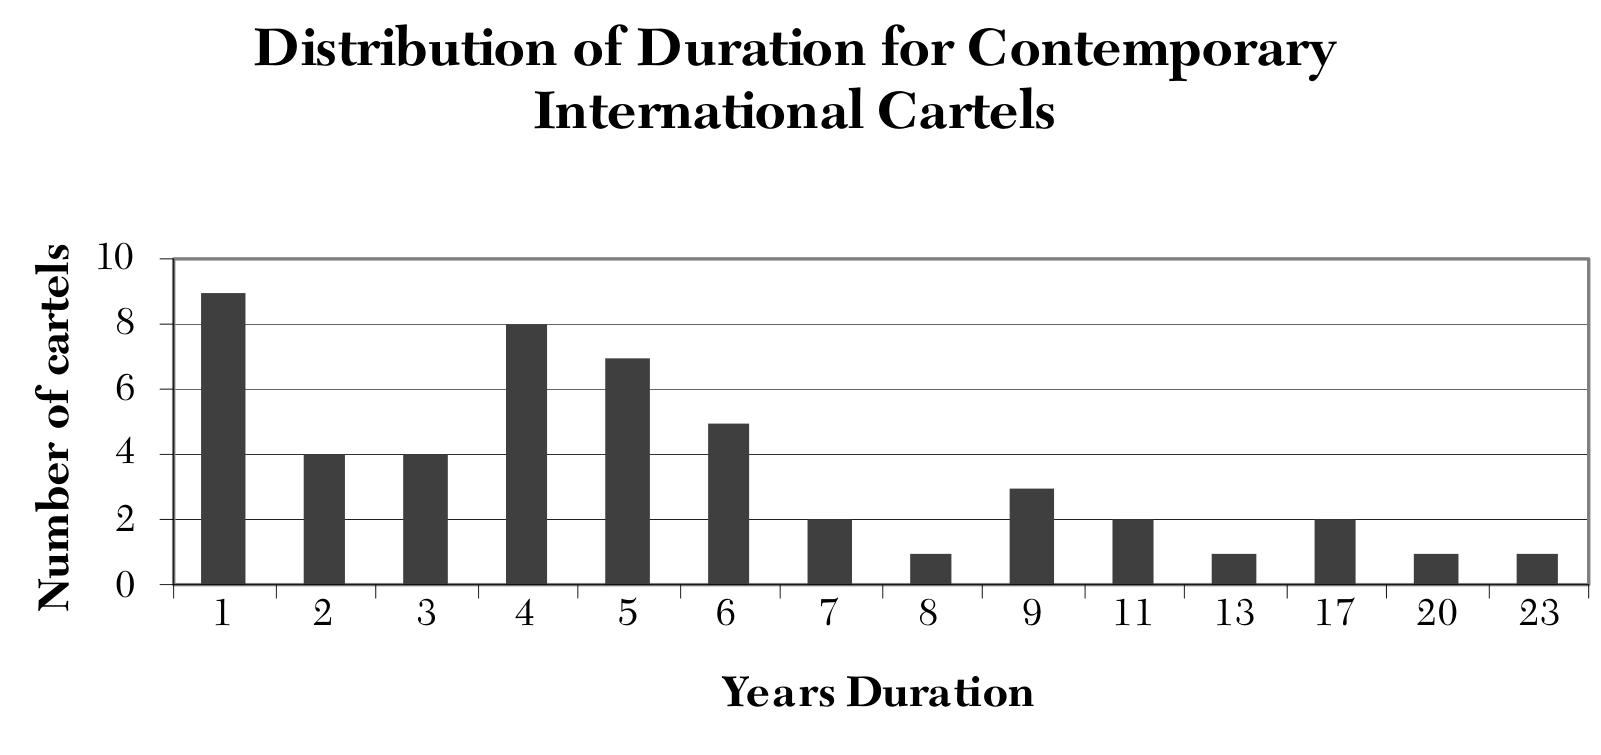
\includegraphics[width=0.78\textwidth]{figures/ch12/ls_fig1.png}
\caption{Distribution of the duration of contemporary international cartels. The horizontal axis lists only the
durations that occur, so it is not to scale. The underlying tabulation is from the authors' 2004 study (their source
note cites ``Levenstein and Suslow (2004b), table 1''). Source: \citet{LevensteinSuslow2006}, Figure~1.}
\label{fig:12-ls-duration}
\end{figure}

Case studies give longer durations (\cref{tab:12-ls-cases}). The nineteen industries contain fifty episodes of
cooperation, with a mean duration of 14 years, a median of 6 years and a standard deviation of 19.6 years
(p.~52). The median is close to the cross-section evidence, while the mean and the dispersion are much larger. The
authors attribute the difference partly to researchers' tendency to study industries with long or eventful cartel
histories. The DeBeers diamond cartel lasted 100 years before its first breakdown, while several cartels in the sample
barely got off the ground (p.~54). The Joint Executive Committee, the most studied cartel in modern economics
(\cref{sec:13-jec}), is the least stable in the sample. Its pools generally lasted two to five years and broke down
through entry or secret cheating (p.~56). Cooperation among southern U.S. railroads lasted three times as long on
average (footnote~40).

\begin{table}[htbp]
\centering
\caption{Cartel duration in selected case studies}\label{tab:12-ls-cases}
\footnotesize
\begin{tabular}{@{}l c r r r r@{}}
\toprule
Industry & First year & Mean duration & Episodes & Maximum & Minimum\\
\midrule
Beer (U.S.) & 1933 & 9 & 1 & 9 & 9\\
Beer (Sweden) & 1894 & 29 & 2 & 50 & 8\\
Bromine & 1885 & 6.25 & 4 & 10 & 3\\
Cement & 1922 & 40 & 1 & 40 & 40\\
Coal & 1893 & 20 & 1 & 20 & 20\\
Diamonds & 1870s & 60 & 2 & 100 & 20\\
Electrical equipment & 1950 & 8 & 1 & 8 & 8\\
Ocean shipping & 1870s & 51 & 3 & 54 & 50\\
Oil & 1871 & 2 & 3 & 3 & 1\\
Parcel post & 1851 & 28.5 & 2 & 40 & 17\\
Potash & 1877 & 9.4 & 8 & 20 & 1\\
Railroad (U.S. Midwest) & 1879 & 1.7 & 3 & 2 & 1\\
Railroad (U.S. South) & 1873 & 5 & 2 & 8 & 1\\
Railroad and oil & 1871 & 7 & 5 & 30 & $<1$\\
Rayon & 1932 & 8 & 1 & 8 & 8\\
Steel (Europe) & 1926 & 7.3 & 4 & 13 & 4\\
Steel (U.S.) & 1933 & 6 & 1 & 6 & 6\\
Sugar & 1887 & 6.75 & 4 & 10 & 2\\
Tea & 1929 & 3.5 & 2 & 6 & 1\\
\bottomrule
\end{tabular}

\smallskip
\begin{minipage}{0.86\textwidth}\footnotesize
Notes: Durations in years. ``First year'' is the first year of the first episode covered by the case studies.
``Episodes'' counts the distinct cartels that the studies date clearly. The episode-weighted mean of the column of
mean durations is 14 years, the figure reported in the text of the survey.
Source: \citet{LevensteinSuslow2006}, Table~2.
\end{minipage}
\end{table}

Is a typical life of five to six years long or short? The authors offer two benchmarks (pp.~56--57). The graphite
electrodes cartel, which lasted from mid-1992 to mid-1997, drew fines of more than 600 million U.S. dollars from U.S. and
European authorities. A cartel of average duration can thus inflict large damage. Firms themselves are not long-lived
either. Geroski reports that 61.5 percent of U.S. entrants exit within five years and 79.6 percent within ten, as
quoted by the authors. Cartels are less than perfectly stable. Yet they are about as durable as many other economic
organizations. The lesson is that cartels cannot be described simply as unstable. Some fail quickly, and others solve
the problems of coordination, cheating and entry for decades.

\subsection{Determinants of cartel duration}\label{sec:12-ls-determinants}

\citet[p.~57]{LevensteinSuslow2006} give two answers to the question of how cartels survive. Surviving cartels operate
in industries whose exogenous features make collusion easier. They also organize themselves to overcome
coordination, cheating and entry. Both are necessary and neither is sufficient.

\casehead{Number of firms and concentration}
The Bertrand constraint predicts that collusion is harder with more firms. The evidence is mixed. Most case-study
cartels and most contemporary international cartels operated in concentrated industries (p.~58). Yet the number of
participants in contemporary international cartels ranged from two to several hundred. Whenever there were more than
about half a dozen firms, an industry association or a government helped organize the agreement. In U.S. price-fixing
cases the mean number of conspirators is 7.25 in the sample of Hay and Kelley, which excludes four cases with 50 or more
conspirators. It is 16.7 in the sample of Fraas and Greer and 29.1 in that of Posner. Gallo et al. report a mean of 2.45 over all
2,689 Commerce Clearing House cases, not only horizontal conspiracies (Table~5). The medians are 7, 8, and
between 6 and 10. The shares of cartels with fewer than ten members are 79, 60 and 64 percent, and the average four-firm
concentration ratio in Hay and Kelley's sample is 77 percent (Table~5).

Effects on duration also conflict (Table~6, p.~61). Dick finds a statistically significant positive effect of the
number of firms on duration. Suslow finds a negative effect, which is not significant, and Hay and Kelley find no
significant pattern. Posner finds that 52 percent of the 79 cases with ten or fewer firms persisted six years or more,
against 64 percent of the 28 cases with more than ten firms. Hay and Kelley do find a positive association between
industry concentration and duration. Most of the conspiracies in their sample that lasted ten years or more were in
highly concentrated markets (Table~6, note~d, and p.~60). More consistently, duration rises with the share of the
market controlled by cartel members. The effect is positive and significant for Dick and Marquez, and positive but
not significant for Suslow. Marquez also finds a significant positive effect of cartel concentration, measured by a
Herfindahl index of the members' shares of cartel output. The authors offer three explanations for the weak link with concentration
(p.~58). Prosecutors may catch large cartels and association-run cartels more easily. Very concentrated industries may
collude tacitly and never appear in samples of explicit cartels. And concentration is endogenous, since collusion lets
more firms survive. Symeonidis finds a concave relation between the prevalence of collusion and concentration across
151 British industries (p.~60).

Trade associations are the organizational answer to large numbers. Posner reports that 44 percent of the cartels in
his sample used an industry association. Hay and Kelley, and Fraas and Greer, find associations in about a third of
U.S. conspiracies (p.~61). In the language of \cref{sec:12-cartels}, an association supplies the communication and
monitoring that large groups cannot achieve tacitly.

\casehead{Large customers}
\citet{Stigler1964} predicted that large buyers would tempt cartel members to cut prices secretly. The only explicit
econometric test, by Dick, finds that Webb-Pomerene export cartels selling to relatively larger buyers dissolved more
quickly (p.~61). Other evidence is less supportive. The citric acid cartel sold to firms such as Mars, Coca-Cola and
Procter \& Gamble, and the vitamins cartel to Kellogg, Quaker Oats and Tyson Foods (p.~62). These buyers do not seem to
have used their resources to break the cartels. The graphite electrodes investigation, started by a steel producer's
complaint, is the one exception the authors know. In five of the nineteen case studies, customers tried to break the
cartel (p.~62 and Table~7). In bromine and potash they tried to integrate backward, and in rayon they spread rumors of
cheating. In other cases customers helped stabilize a cartel and shared its rents. Customer size may destabilize a
cartel, while customer concentration may have the opposite effect.

\casehead{Demand}
Eckbo finds that cartels raised prices substantially only when demand was sufficiently inelastic with few short-run
substitutes (p.~64). The brewing industry, with a demand elasticity of $-10.3$, had an unsuccessful cartel,
with price wars in every year of the study (p.~64 and Table~8).

Demand instability matters more than the business cycle as such (Table~9). Dick finds that instability shortens
Webb-Pomerene cartels and that anticipated downturns end them, while unanticipated cycles have no significant
effect. Suslow finds significant negative effects of demand growth, of the business cycle and of unanticipated cycles.
Marquez finds a negative but insignificant effect of demand growth. Across case studies, macroeconomic fluctuations
seem to have had little relevance (p.~67 and Table~10). The international steel cartel is the only one reported to
have collapsed because of an observable demand shock. The authors read this as consistent with the Green-Porter and
Abreu literature, in which price wars follow unobserved rather than observed fluctuations. Their conclusion is that
unanticipated shocks and very rapid growth undermine cartels, while predictable cyclical fluctuations do not (p.~86).

This evidence must be mapped to the theory with care. The theories of \cref{sec:12-demand,sec:12-public} predict
changes in collusive prices or temporary price wars, not the end of a cartel. A Green-Porter reversion would appear as
a breakdown only if the researcher dates episodes by price wars. The finding that anticipated downturns end
Webb-Pomerene cartels fits the logic of \citet{HaltiwangerHarrington1991} and \citet{BagwellStaiger1997}, in which
collusion is hardest when future demand looks weak. It does not test whether the cartels died or merely punished.

\casehead{Organization and learning}
Successful cartels build organizations that monitor members, adjust the agreement to changing conditions, and settle
disputes (pp.~67--74). A joint sales agency is the strongest form, since it removes each firm's discretion over price.
Seven of the nineteen case-study industries used one: bromine, cement, diamonds, ocean shipping, oil, potash and
European steel. Most of these were among the more successful cartels (p.~69). Dick finds that a single sales agent
lowers the likelihood of cartel failure. Table~11 of the survey covers four U.S. cross-sections: Hay and Kelley,
Fraas and Greer, Posner, and Gallo et al. Trade associations were involved in 29, 36, 44 and 23 percent of their cases,
and market allocation in 35, 26, 26 and 27 percent. Suslow finds that self-imposed penalties significantly lengthen
cartel life (p.~71).

Hierarchies separate policy from day-to-day management. In the electrical equipment conspiracy of the 1950s, a working
group of sales managers devised the ``phases of the moon'' formula. It rotated the winning bidder for switchgear orders
every two weeks (pp.~72--73). In the citric acid cartel of 1991 to 1995, senior executives, nicknamed ``the
masters,'' set the broad agreement. Lower-level ``sherpas'' ran it. They shared monthly sales figures, and a firm that
sold more than its quota had to buy citric acid from a member below quota the next year (p.~73). This is the
quota-and-transfer scheme that \citet{HarringtonSkrzypacz2011} rationalize (\cref{thm:12-hs}).

Cartels learn. Dick and Suslow both find that prior cartel experience lengthens duration (Table~12). Within a single
episode, Dick finds that the hazard of dissolution rises with age. A cartel in its tenth year was 28 to 48 percent more
likely to dissolve than one in its fifth year. Several case-study cartels got off to a rocky start and later lasted for
long periods. Swedish brewers formed a cartel in 1894 with better control machinery than earlier attempts, and a
cartel formed in 1906 lasted fifty years (p.~74).

\casehead{Entry and exclusion}
Entry is a central threat. Dick finds that export associations formed where entry was slow, and Symeonidis that
collusion is more likely in capital-intensive industries (p.~74). Successful cartels create barriers to entry. Scott
Morton documents 47 cases of attempted entry against British shipping cartels. A typical price war against an entrant
lasted three months and cut prices by 50 percent on the routes the entrant served (p.~75). Nineteenth-century U.S. salt
producers, by contrast, saw each collusive arrangement collapse within a year or two because entry barriers were too
low (pp.~74--75).

\subsection{Why cartels break down}\label{sec:12-ls-breakdown-causes}

\Cref{tab:12-ls-breakdown} reproduces the causes of breakdown in international cross-sections. In Eckbo's first
sample, internal conflict or defection ended ten of twenty-three cartels, roughly 44 percent, and in his second sample
59 percent (p.~75). In Suslow's sample about a quarter ended because of internal conflict and cheating. Only World
War~II ended a larger share. Griffin finds that half of his cartels ended for political or external reasons
(p.~76). Entry or substitutes contributed to a third of his failures, and ``behavioral problems'' to another third. World War~II ended twelve of his cartels, and technological change ended four (rubber, zinc, sulfur and
nitrate). The category ``cheating and disagreement'' mixes monitoring failures with bargaining failures, which the
theory treats very differently.

\begin{table}[htbp]
\centering
\caption{Causes of cartel breakdown in international cross-section studies (percent of episodes)}\label{tab:12-ls-breakdown}
\footnotesize
\begin{tabular}{@{}l r r r r@{}}
\toprule
Cause of breakdown & Eckbo, sample 1 & Eckbo, sample 2 & Griffin$^{a}$ & Suslow\\
\midrule
Cheating and disagreement & 43.5 & 58.6 & 33.3 & 23.9\\
External shock & 30.4 & & 50.0$^{c}$ & 42.3\\
Entry and substitution$^{b}$ & 26.1 & 41.4 & 33.3 & 15.5\\
\quad Entry & 13.0$^{b}$ & & 25.9 & 15.5\\
\quad Substitution & 8.7$^{b}$ & & 9.3 & \\
Technological change & & & 9.3 & \\
Antitrust indictment & & & & 18.3\\
\midrule
Total number of episodes & 23 & 29 & 54 & 71\\
\bottomrule
\end{tabular}

\smallskip
\begin{minipage}{0.92\textwidth}\footnotesize
Notes: Blank cells are not reported. (a) Based on Griffin's discussion and on his Table~4. Griffin lists more than one
cause for several cartels, so his column sums to more than 100. The survey's text names four cartels ended by
technological change (4 of 54, or 7.4 percent), while the table reports 9.3 percent. Its footnote~90 notes that
Griffin's own text and table differ. We reproduce both figures as printed. (b) Entry and substitution do not always add to the
total, because Eckbo leaves one episode unclassified and Griffin counts two cartels under both. Of Eckbo's six
episodes in this category, three ended through entry, two through substitution and one is unclassified. (c) Griffin
groups wars, antitrust and other government actions, and cartel reorganizations. Some reorganizations may be
bargaining problems, so the entry overstates external shocks as classified here.
Source: \citet{LevensteinSuslow2006}, Table~13.
\end{minipage}
\end{table}

Case studies separate these causes better (Table~14 of the survey, p.~77). Entry was the primary cause of
disruption in just over a third of the episodes. World Wars~I and~II ended about 15 percent and legal action a little
over 10 percent. Only three episodes, fewer than 10 percent, ended because of cheating (p.~78). Bargaining problems
affected virtually every cartel and ended about a quarter of the episodes. Many case-study authors report that
cheating was simply not a problem.

Successful cartels avoided costly punishments. The Sugar Institute ``served as a court in which an accused firm might
prove its innocence'' \citep[p.~389]{GenesoveMullin2001}, as quoted by \citet[p.~78]{LevensteinSuslow2006}. Outside
the South, deviations ``were either ignored or matched'' rather than met by reversion to competition
\citep[pp.~390--391]{GenesoveMullin2001} (see \cref{sec:13-sugar-institute}). In steel in the 1930s, unexpected
declines in demand led to ``shallow episodes of increased competition,'' in Baker's words, rather than severe price
wars. In bromine, violations were answered with negotiated side payments rather than price wars
(\citealp{Levenstein1997}, \cref{sec:13-bromine}). The authors conclude that Cournot reversion is an inefficient way to
sustain collusion, as the cartel members themselves repeatedly discovered (p.~78).

\citet[p.~79]{LevensteinSuslow2006} draw three lessons. First, the outbreak of a price war, as opposed to its threat,
is rarely a sign of cartel success. Second, the most successful cartels develop alternative punishments and threats
that sustain collusion at lower cost. Third, cartels break down sometimes because of cheating, but more often because
of entry, exogenous shocks and dynamic changes within the industry.

\subsection{Effects on prices}\label{sec:12-ls-prices}

Rigorous counterfactual estimates of cartel overcharges are rare (p.~45). The available evidence nonetheless shows that
many cartels raised prices substantially (pp.~80--81). Eckbo finds that nineteen of fifty-one cartels raised price 200
percent above the unit cost of production and distribution. Griffin finds an average markup of 45 percent over marginal
cost. His most successful cartel, rubber from 1923 to 1928, had a markup of 400 percent, while his least successful,
wheat from 1933 to 1934, priced below cost. For contemporary international cartels, reported price increases, mostly
from the trade press, range from 10 to 100 percent. Graphite electrode prices rose more than 50 percent in the United
States from 1992 to 1997. In Canada, where two firms held more than 90 percent of the market, they rose more than 90
percent. Some evidence points the other way. Fölster and Peltzman find that legal Swedish cartels did not raise prices,
although a re-examination of the same data by Ciarreta finds that they did. In 25 price-fixing cases from 1973 to 1984,
Sproul finds that prices four years after indictment were slightly higher, by 7 percent.

Case studies seldom measure success against a counterfactual (p.~81 and Table~15). Hausman finds that the regulations
of the ``Limitation of the Vend,'' a coal cartel in northeast England from 1770 to 1845, raised the equilibrium price
by about 6 to 8 percent. Bromine prices came close to the joint-profit-maximizing level in some periods and barely
exceeded the Cournot level in others. Ocean shipping was close to the joint-profit level. The German steel cartel
priced below the joint-profit level but one-third above the world price. The cement cartel priced 10 percent above
the world price. Diamond prices nearly doubled after the cartel formed, and tea prices rose 80 percent
in 1933 after the cartel was reestablished. The U.S. beer cartel of the 1930s may even have priced above the monopoly
level, under political pressure to keep alcohol expensive. Yet it had price wars in each of the three years it tried
to collude. Success must be judged over the whole life of a cartel, not only during its collusive periods (p.~81). The
methods for estimating overcharges and damages are developed in \cref{sec:13-damages}.

\subsection{What the evidence says about the theory}\label{sec:12-ls-theory}

The survey speaks to each part of the theory in this chapter.
\begin{enumerate}[label=(\arabic*)]
\item \emph{Structure.} The perfect-monitoring theory of \cref{sec:12-perfect} predicts that collusion is easier with
fewer firms. Concentration helps, but organization can substitute for it, and concentration is itself shaped by
collusion.
\item \emph{Demand.} Unanticipated shocks and rapid growth undermine cartels, while predictable cycles do not. This
pattern matches the role of unobserved shocks in \citet{GreenPorter1984}. The evidence on anticipated downturns fits
the persistent-demand models of \cref{sec:12-demand}. Cross-section data on cartel deaths cannot test the
within-cartel price dynamics these models predict. That requires the time-series studies of \cref{sec:13-jec}.
\item \emph{Price wars.} Many observed price wars are bargaining wars or breakdowns. Successful cartels prefer
monitoring, courts and side payments to Green-Porter reversions. This supports the shift of the theory toward
communication and transfers (\cref{sec:12-cartels}) and toward tolerated cheating (\cref{rem:12-bm},
\cref{sec:13-imperfect}).
\item \emph{Organization.} Joint sales agencies, reporting systems, penalties and hierarchies lengthen cartel life.
Theory treats them as devices that make information public or transfers possible, as in
\citet{HarringtonSkrzypacz2011}.
\item \emph{Entry.} Entry is the most common cause of breakdown in the case studies, yet most repeated-game models
hold the set of firms fixed. This is the largest gap between the theory and the evidence.
\item \emph{Enforcement.} Antitrust action ended 18.3 percent of Suslow's interwar international cartels and a little
over 10 percent of case-study episodes. Enforcement also selects which cartels we observe, as \cref{sec:12-enforcement}
and \cref{sec:13-institutions} discuss.
\end{enumerate}

The survey has limits. It aggregates studies with different definitions of a cartel, of an episode and of a cause of
breakdown. Most of its quantitative statements are counts and percentages, not estimates with standard errors. Selection
is unavoidable and of unknown sign. The cross-section regressions it summarizes use duration as the dependent variable,
which is a noisy measure of success, and they rarely control for the endogeneity of structure and organization. Its
contribution is to replace the presumption that cartels are inherently unstable with a set of facts. Cartels often
last for years. They end more often through entry, shocks and bargaining than through secret cheating. The successful
ones invest in organization.

\section{Synthesis: What the Theory Predicts and How to Test It}\label{sec:12-synthesis}

\Cref{tab:12-models} collects the models of this chapter. Each row states what firms observe, why collusion is hard,
what the most collusive equilibrium looks like, whether price wars occur on the equilibrium path, and what the model
predicts for prices. The last column points to the section of \cref{ch:collusion-evidence} where the prediction meets
data.

The table carries five lessons for empirical work.

The first lesson is that theory delivers a set of sustainable outcomes and leaves the choice among them open. The
folk theorem and
\cref{cor:12-bertrand-any-price} imply that a wide range of prices can be sustained in the same environment. Empirical
work that tests ``collusion'' must therefore commit to a specific model of how the cartel operates. The common
selection, the most collusive equilibrium, is a convention.

The second lesson is that conduct varies over time. In Rotemberg and Saloner, Haltiwanger and Harrington, and Bagwell
and Staiger, collusive margins move with current and expected demand. In Green and Porter, conduct switches between
regimes. A constant conduct parameter then averages over states, which is the critique of \citet{Corts1999} discussed
in \cref{ch:conduct}. Estimation must allow for regimes or for state-dependent conduct, as the methods of
\cref{sec:13-implications} do.

The third lesson is that a price war is an ambiguous signal. In \citet{GreenPorter1984} it is part of a working
cartel. In \citet{Stigler1964} and in the bargaining wars documented by \citet{LevensteinSuslow2006}, it marks a
failing one. The timing of wars relative to demand helps discriminate. Wars after unexpected drops in demand point to
Green and Porter. Low prices in booms point to Rotemberg and Saloner. Wars around entry or renegotiation point to
bargaining. \Citet{Ellison1994} uses exactly this logic to test Green and Porter against Rotemberg and Saloner in the
railroad cartel of \citet{Porter1983} (\cref{sec:13-ellison}).

The fourth lesson is that communication and transfers are observable in prosecuted cartels, and they matter most when
information is private. The anatomy of the lysine and citric acid cartels, with quotas, sales reports and buy-backs, is
predicted by \citet{HarringtonSkrzypacz2011}. The identical bidding of many rings is predicted by
\citet{AtheyBagwellSanchirico2004}, and their take-turns scheme is a model of bid rotation. Evidence on the internal organization of cartels can thus discriminate among
models in a way that price data alone cannot.

The fifth lesson is that detection needs a competitive benchmark and a theory of the specific cartel. Overcharges are
measured against a but-for price. Tests of bid rigging compare suspected firms with a model of noncooperative bidding.
Enforcement determines which cartels enter the data, so every finding is conditional on how the cartels were found.

\begin{landscape}
\begin{table}[p]
\centering
\caption{Models of collusion and their testable implications}\label{tab:12-models}
\scriptsize
\renewcommand{\arraystretch}{1.1}
\begin{tabularx}{\linewidth}{@{}>{\raggedright\arraybackslash}p{2.5cm}
>{\raggedright\arraybackslash}X >{\raggedright\arraybackslash}X >{\raggedright\arraybackslash}X
>{\raggedright\arraybackslash}p{2.7cm} >{\raggedright\arraybackslash}X
>{\raggedright\arraybackslash}p{2.1cm}@{}}
\toprule
Model & What firms observe & Source of the incentive problem & Most collusive equilibrium and price pattern & Price
wars on the path? & Testable implication & Tested in\\
\midrule
Perfect monitoring, Bertrand and Cournot (\cref{sec:12-perfect}) & All past prices or outputs & One-period gain from
undercutting against the loss of future collusion & Stationary price, monopoly if $\delta \ge \underline\delta(N)$.
Any price in $[c, p^m]$ can be sustained & No & Collusion is easier with fewer, more symmetric firms, frequent
interaction and transparency & \cref{sec:13-information}, \cref{ch:mergers}\\
Rotemberg and Saloner (\cref{sec:12-demand}) & Current demand (\iid) and past prices & Gain from cheating rises with
current demand, future loss is constant & Monopoly price in low states, capped profit in high states. Countercyclical
margins & No, unless prices are restricted to collude or compete & Margins fall when current demand is high relative
to expected demand & \cref{sec:13-jec}, \cref{sec:13-gasoline}\\
Haltiwanger and Harrington (\cref{sec:12-demand}) & A known demand cycle & Future loss is small when demand is about
to fall & Prices lowest when demand is about to fall, and at the peak only for impatient firms & No & Margins rise with expected future demand &
\cref{sec:13-gasoline}\\
Bagwell and Staiger (\cref{sec:12-demand}) & Current growth phase (Markov) & Gain and loss both move with the phase &
Procyclical prices if growth rates are positively correlated, countercyclical if negatively & No & Cyclicality
depends on the persistence and expected durations of phases & \cref{sec:13-predictions}\\
Green and Porter (\cref{sec:12-public}) & Market price only & A low price may reflect cheating or low demand &
Trigger price, reversion of finite length. Regime switching & Yes, after unexpectedly low prices & Wars follow
negative demand shocks and have finite length & \cref{sec:13-jec}\\
Athey, Bagwell and Sanchirico (\cref{sec:12-private-costs}) & Public prices, private \iid\ costs & Low-cost firms want
more market share & Patient firms: one rigid price, equal shares. Impatient firms: an escape clause & No (inelastic
demand) & Rigid, identical prices that ignore firm-specific costs & \cref{sec:13-detection}, \cref{sec:13-legal}\\
Harrington and Skrzypacz (\cref{sec:12-cartels}) & Own sales and public reports & Secret price cuts, unverifiable
sales reports & Quotas, sales reports and per-unit transfers. Breakdown after low total reports & Yes, rare
breakdowns & Quota schemes with buy-backs, breakdowns after low sales & \cref{sec:13-imperfect}\\
Bernheim and Madsen (\cref{rem:12-bm}) & All quotes, with costly quoting and home cost advantages & Raiding the
rival's home market & Price floor below the home monopoly price. Dispersed prices & No. Raids above the floor are
tolerated & Business stolen at higher prices is less likely to be punished & \cref{sec:13-imperfect}\\
Chen and Rey (\cref{sec:12-chenrey}) & Own conduct, random detection, leniency & Cheat and report, or collude and
report & Normal collusion if the stake exceeds the deterrence threshold & No (binary conduct) & Excessive leniency
induces systematic self-reporting & \cref{sec:13-enforcement}, \cref{sec:13-asker}\\
\bottomrule
\end{tabularx}

\smallskip
\begin{minipage}{\linewidth}\scriptsize
Notes: Our synthesis of the models in this chapter. \citet{BernheimMadsen2017} is developed in
\cref{sec:13-imperfect}. Price wars on the path refer to the most collusive equilibrium of each model.
\end{minipage}
\end{table}
\end{landscape}

\Cref{ch:collusion-evidence} takes these lessons to data. It begins with the econometrics of regime switching
(\cref{sec:13-implications}) and the Joint Executive Committee (\cref{sec:13-jec}), where the Green-Porter and
Rotemberg-Saloner predictions are tested. It continues with the rules and communication of legal cartels, information
exchange, retail gasoline, tolerated cheating, the internal organization of a bidding ring, and the statistical
detection of bid rigging. It ends with enforcement and the measurement of damages (\cref{sec:13-enforcement}).


\section{Bibliographic notes}\label{sec:12-bibnotes}

The modern theory of collusion begins with \citet{Stigler1964}, who saw a cartel's central problem as the
detection of secret price cuts. \citet{Friedman1971} showed that the threat of reverting to static Nash play
sustains collusion as a noncooperative equilibrium of a supergame. \citet{FudenbergMaskin1986} proved the folk
theorem with minmax punishments, and \citet{Abreu1986,Abreu1988} characterized optimal punishments and simple
penal codes. \citet{FarrellMaskin1989} asked which punishments survive renegotiation. \citet{BenoitKrishna1985}
and \citet{KrepsEtAl1982} showed how multiple stage equilibria and incomplete information restore cooperation in
finitely repeated games. \citet{BrockScheinkman1985} and \citet{CompteJennyRey2002} added capacity constraints.
\citet{FudenbergTirole1991} and \citet{MailathSamuelson2006} are the standard references for the theory of repeated
games. Chapter~6 of \citet{Tirole1988} remains the classic textbook treatment of its applications to oligopoly,
including the kinked demand curve and the alternating-move model of \citet{MaskinTirole1988}.
\citet{AskerNocke2021} survey the modern literature on collusion in the Handbook of Industrial Organization. They
cover the prevalence of cartels, how agreements start and are structured, imperfect monitoring, multimarket contact,
entry and detection.

\citet{GreenPorter1984} brought imperfect public monitoring into the theory of collusion and showed that price wars
can be part of a working cartel. \citet{Porter1983b} studied optimal trigger strategies.
\citet{AbreuPearceStacchetti1986,AbreuPearceStacchetti1990} developed the recursive methods that now dominate the
field, and \citet{FudenbergLevineMaskin1994} proved a folk theorem for games with imperfect public monitoring.
Collusion under fluctuating demand starts with \citet{RotembergSaloner1986}, whose working paper
\citep{RotembergSaloner1984} contains the evidence. \citet{HaltiwangerHarrington1991}, \citet{Kandori1991},
\citet{StaigerWolak1992} and \citet{BagwellStaiger1997} studied persistent demand, correlated shocks and capacity.

Private information about costs entered with \citet{AtheyBagwell2001} and \citet{AtheyBagwellSanchirico2004}, and
\citet{AtheyBagwell2008} allowed costs to be persistent. \citet{McAfeeMcMillan1992} analyzed bidding rings with
and without side payments. The theory of private monitoring and communication includes \citet{Compte1998} and
\citet{KandoriMatsushima1998}. \citet{HarringtonSkrzypacz2007,HarringtonSkrzypacz2011} connected it to the
practices of prosecuted cartels, and \citet{AwayaKrishna2016} studied when cheap talk about sales helps.
\citet{BernheimMadsen2017} explained why cartels tolerate some cheating. \citet{BernheimWhinston1990} is the classic
analysis of multimarket contact, and \citet{Matsushima2001} extended it to imperfect monitoring.
\citet{SugayaWolitzky2018} showed that more information can hinder collusion. \citet{BosHarrington2010} studied which
firms join a cartel. \citet{ByrneDeRoos2019} documented how firms learn to coordinate tacitly, and
\citet{CalvanoEtAl2020} opened the study of collusion by pricing algorithms.

On enforcement, \citet{MottaPolo2003} and \citet{Spagnolo2004} began the economic analysis of leniency programs.
\citet{AubertReyKovacic2006} studied rewards to individual informants, \citet{Harrington2008} the race to report,
and \citet{ChenRey2013} the optimal design of a program. \citet{Miller2009} measured the effect of the 1993 U.S.
revision on detection and deterrence. \citet{Kaplow2013} questions the agreement requirement on which enforcement
rests. His chapters~2, 3 and 7 examine the meaning of agreement, the role of communication and the link between
equilibrium and agreement. \citet{MarshallMarx2012} give a book-length account of how cartels and bidding rings are
organized, of when explicit collusion is needed, and of the plus factors that reveal it. \citet{KawaiNakabayashi2020}
and \citet{ConleyDecarolis2016} estimate how widespread collusion is in public procurement. \citet{LevensteinSuslow2006}
survey the evidence on cartel duration, organization and breakdown, which \cref{ch:collusion-evidence} develops
further.

\section{Exercises}\label{sec:12-exercises}

\begin{enumerate}[label=\arabic*., leftmargin=*, itemsep=6pt]

\item \textit{Detection lags.} A deviation is detected only $k$ periods after it starts.
\begin{enumerate}[label=(\alph*)]
  \item Extend \cref{prop:12-bertrand-ext} to the linear Cournot supergame of \cref{prop:12-cournot}: show that with
  a $k$-period detection lag, grim trigger sustains $q^m$ if and only if $\delta^k \ge \delta^*(N)$.
  \item In the Bertrand supergame with demand growth, use \eqref{eq:12-bertrand-ext} to compute the threshold for
  $N = 4$, $k = 2$ and $g = 0.05$, and compare it with the value for $g = 0$. You should find about 0.825 and about
  0.866.
  \item Let $N = 4$, $\delta = 0.8$ and $g = 0$. Find the longest detection lag that a Cournot cartel can tolerate,
  and the longest that a Bertrand cartel can tolerate. You should find $k = 2$ and $k = 1$. Explain what the
  difference implies for the value to each cartel of exchanging sales reports.
\end{enumerate}

\item \textit{Capacity constraints.} Three firms with zero marginal cost face demand $D(p) = 1 - p$. Each can produce
at most $K$ units per period, with $\frac{1}{6} < K < \frac{1}{2}$. Rationing is efficient. Assume that a deviator
can be held to its minmax payoff in every period after a deviation.
\begin{enumerate}[label=(\alph*)]
  \item Show that the best deviation from collusion at $p^m = \frac{1}{2}$ earns almost $\frac{K}{2}$.
  \item Show that the minmax payoff is $K(1 - 3K)$ for $K \le \frac{1}{4}$ and $\frac{(1 - 2K)^2}{4}$ for
  $K \ge \frac{1}{4}$.
  \item Use the bound of \cref{ex:12-capacity} to show that the threshold discount factor is $\frac{1}{6K}$ for
  $K \le \frac{1}{4}$ and $\frac{6K - 1}{18K - 12K^2 - 3}$ for $K \ge \frac{1}{4}$.
  \item Show that the threshold falls with $K$ up to $K = \frac{1}{3}$, where it equals $\frac{3}{5}$, and rises
  afterward toward $\frac{2}{3}$, the value without capacity constraints. Explain the two forces at work.
\end{enumerate}

\item \textit{Stick and carrot with three firms.} Three Cournot firms face $P(Q) = a - bQ$ at every output and have
marginal cost $c < a$.
\begin{enumerate}[label=(\alph*)]
  \item Set $a - c = b = 1$. Show that the carrot and stick constraints of \cref{prop:12-abreu-two-phase} become
  $\frac{1}{36} \le \delta\frac{(6x - 1)^2}{12}$ and $\frac{(4x - 1)^2}{4} \le \delta\frac{(6x - 1)^2}{12}$.
  \item Show that the best stick output is $x = \frac{a - c}{3b}$ per firm, that the stick drives the price down to
  marginal cost, and that monopoly sharing is sustainable for $\delta \ge \frac{1}{3}$. Compare this with the
  threshold $\frac{4}{7}$ under Nash reversion.
  \item Explain why the stick constraint must bind at the optimum. Would the answer change if the price could not
  fall below zero and $c$ were close to zero (\cref{rem:12-abreu-floor})?
\end{enumerate}

\item \textit{Booms of different frequency.} Modify the two-state model of \cref{asm:12-two-state} so that the high
state occurs with probability $\mu \in (0, 1)$.
\begin{enumerate}[label=(\alph*)]
  \item Show that the incentive constraints become $\pi_s(p_s) \le \kappa[\mu\pi_H(p_H) + (1 - \mu)\pi_L(p_L)]$ for
  $s = H, L$, with $\kappa$ as in \eqref{eq:12-kappa}.
  \item Use \cref{lem:12-two-constraint} to show that some collusion is possible if and only if $\kappa \ge 1$,
  whatever $\mu$. Show that monopoly pricing in both states requires
  $\kappa \ge \bar\kappa(\mu) \equiv \frac{\pi_H^M}{\mu\pi_H^M + (1 - \mu)\pi_L^M}$.
  \item In the intermediate regime, show that $p_L = p_L^M$ and
  $\pi_H(p_H) = \frac{\kappa(1 - \mu)\pi_L^M}{1 - \kappa\mu}$.
  \item With $D_s(p) = A_s(1 - p)$, $c = 0$, $A_H = 1.5$, $A_L = 1$, $\mu = \frac{1}{3}$ and $N = 2$, compute
  $\bar\kappa$ and $\bar\delta$, and the boom price at $\kappa = 1.1$. You should find $\bar\kappa = \frac{9}{7}$,
  $\bar\delta = \frac{9}{16}$ and $p_H \approx 0.261$. Explain why rarer booms widen the range of discount factors
  with countercyclical prices.
\end{enumerate}

\item \textit{Noise and the length of price wars.} Use the Bertrand version of Green and Porter
(\cref{asm:12-gp-bertrand}) with $\delta = 0.95$ and $\gamma = 0.2$.
\begin{enumerate}[label=(\alph*)]
  \item Find the shortest war $T^*$ that satisfies \eqref{eq:12-gp-ic}, and the long-run share of periods spent in
  wars. You should find $T^* = 2$ and $\frac{2}{7}$.
  \item Compute the value of collusion $V$ at $T^*$ and with an infinite war. Explain why the cartel prefers the
  shorter war although it punishes less.
  \item An econometrician observes many wars in this industry. Explain why the observation, by itself, is not
  evidence that the cartel is breaking down. What additional data would distinguish this model from
  \citet{RotembergSaloner1986}?
  \item Now let $N$ firms play the noisy-signal model of \cref{prop:12-an}, with the same $\delta$ and $\gamma$ and with
  $\lambda = 1$. For $N = 2$, 3 and 4, compute the threshold \eqref{eq:12-an-delta}, the punishment probability
  $\phi^*$ and the ratio of $v^*$ to $\frac{\bar\pi}{N}$. You should find ratios of 0.75, 0.5 and 0.25. Explain why the
  number of firms matters although $\delta$ exceeds every threshold. For $N = 2$, compare $v^*$ with $(1 - \delta)V$ at
  $T^*$ from part (b), and explain why a random punishment can do better than the best war of integer length.
\end{enumerate}

\item \textit{Cost dispersion and rigid prices.} Two firms have private costs drawn independently from the uniform
distribution on $[0, \bar c]$, with $0 < \bar c \le 1$. Demand is inelastic with reservation value $\bar v = 1$.
\begin{enumerate}[label=(\alph*)]
  \item Show that the static equilibrium is $p^e(c) = c + \frac{\bar c - c}{2}$ and that the ex ante profit per
  firm is $\frac{\bar c}{6}$.
  \item With Nash reversion after an off-schedule price, use \cref{prop:12-abs-critical} to show that the rigid
  price $\bar v$ is sustainable if and only if $\delta \ge \delta^* = \frac{1}{2 - \frac{5\bar c}{6}}$. Check that
  $\delta^* = \frac{6}{7}$ for $\bar c = 1$ and that $\delta^* \to \frac{1}{2}$ as $\bar c \to 0$.
  \item Compute $\delta^*$ when the war gives zero profit instead of Nash profit, for $\bar c = 1$. Explain why
  dispersion in costs makes collusion harder even with the harshest punishment.
  \item Explain why patient firms with these costs prefer a rigid price to any fully sorting scheme, and why
  impatient firms may use an escape clause.
\end{enumerate}

\item \textit{Transfers in quota cartels.}
\begin{enumerate}[label=(\alph*)]
  \item In the model of \cref{sec:12-hs}, suppose that each firm pays $z$ per unit of reported sales into a common
  fund that is shared equally among all $N$ firms, the payer included. Show that the effective marginal cost is
  $c + z$, and compare it with $c + \frac{N}{N-1}z$ in \cref{prop:12-hs-cost}. Which design deters business stealing
  more for a given payment?
  \item Let $N = 4$, let the static markup be constant, and let market demand be uniform on $\{60, \dots, 100\}$.
  Check condition \eqref{eq:12-hs-cond2}. Show that the scheme retains a quarter of the first-best collusive gain
  and that $\beta_{\min} = \frac{0.15}{\delta}$.
  \item Compute the expected breakdown probability per period and the mean length of the collusive phase for
  $\delta = 0.95$ and $\delta = 0.99$. Compare the answers with \cref{ex:12-hs-numbers} and explain why more
  volatile demand raises the cost of truthful reporting.
\end{enumerate}

\item \textit{Leniency with more firms.}
\begin{enumerate}[label=(\alph*)]
  \item Fill in the derivations behind \cref{rem:12-cr-nfirms}: derive the thresholds $B_N^r(\ell)$ and
  $B_R(\ell)$ for $N$ firms, and the optimal amnesty rate $\hat\ell_N$.
  \item For $\delta = 0.8$ and $\varrho = 0.4$, show that $\hat\ell_2 = 1$ and $\hat B_2 = \frac{2}{3}F$, and
  compute $\hat\ell_3$. Explain why larger cartels call for more generous leniency.
  \item In the laboratory treatment of \citet{HinloopenSoetevent2008} with $\ell = 1.8$, explain why many subjects
  colluded and reported in every period.
  \item Explain why leniency is useless without the first-informant rule (\cref{rem:12-first-informant}).
\end{enumerate}

\end{enumerate}
